%%%%%%%%%%%%%%%%%%%%%%%%%%%%%%%%%%%%%%%%%
% kaobook
% LaTeX Template
% Version 1.2 (4/1/2020)
%
% This template originates from:
% https://www.LaTeXTemplates.com
%
% For the latest template development version and to make contributions:
% https://github.com/fmarotta/kaobook
%
% Authors:
% Federico Marotta (federicomarotta@mail.com)
% Based on the doctoral thesis of Ken Arroyo Ohori (https://3d.bk.tudelft.nl/ken/en)
% and on the Tufte-LaTeX class.
% Modified for LaTeX Templates by Vel (vel@latextemplates.com)
%
% License:
% CC0 1.0 Universal (see included MANIFEST.md file)
%
%%%%%%%%%%%%%%%%%%%%%%%%%%%%%%%%%%%%%%%%%

%----------------------------------------------------------------------------------------
%	PACKAGES AND OTHER DOCUMENT CONFIGURATIONS
%----------------------------------------------------------------------------------------

\documentclass[
    a4paper, % Page size
    fontsize=10pt, % Base font size
    twoside=true, % Use different layouts for even and odd pages (in particular, if twoside=true, the margin column will be always on the outside)
	%open=any, % If twoside=true, uncomment this to force new chapters to start on any page, not only on right (odd) pages
	%chapterentrydots=true, % Uncomment to output dots from the chapter name to the page number in the table of contents
	numbers=noenddot, % Comment to output dots after chapter numbers; the most common values for this option are: enddot, noenddot and auto (see the KOMAScript documentation for an in-depth explanation)
]{kaobook}

% Set the language
\usepackage[english]{babel} % Load characters and hyphenation
\usepackage[english=british]{csquotes} % English quotes

\setcounter{margintocdepth}{\sectiontocdepth}


% Load packages for testing
\usepackage{blindtext}
%\usepackage{showframe} % Uncomment to show boxes around the text area, margin, header and footer
%\usepackage{showlabels} % Uncomment to output the content of \label commands to the document where they are used
\usepackage{graphicx}
\usepackage[percent]{overpic}
\usepackage[utf8]{inputenc}
% \usepackage{natbib}
\usepackage{amsmath}
\usepackage{siunitx}
\sisetup{group-separator = {,}}
\usepackage{subcaption}
\usepackage{todonotes}
\usepackage[version=4]{mhchem}
\usepackage{wasysym}
\usepackage{overpic}
\usepackage{lipsum}
\usepackage[dvipsnames]{xcolor}
\usepackage{calrsfs}

% package for code blocks
\usepackage{listings}

\DeclareMathAlphabet{\pazocal}{OMS}{zplm}{m}{n}
\newcommand{\Aa}{\mathcal{A}}
\newcommand{\Ab}{\pazocal{A}}

\definecolor{codegreen}{rgb}{0,0.6,0}
\definecolor{codegray}{rgb}{0.5,0.5,0.5}
\definecolor{codepurple}{rgb}{0.58,0,0.82}
\definecolor{backcolour}{rgb}{0.95,0.95,0.92}

\lstdefinestyle{mystyle}{
    backgroundcolor=\color{backcolour},   
    commentstyle=\color{codegreen},
    keywordstyle=\color{magenta},
    numberstyle=\tiny\color{codegray},
    stringstyle=\color{codepurple},
    basicstyle=\ttfamily\footnotesize,
    breakatwhitespace=false,         
    breaklines=true,                 
    captionpos=b,                    
    keepspaces=true,                 
    numbers=left,                    
    numbersep=5pt,                  
    showspaces=false,                
    showstringspaces=false,
    showtabs=false,                  
    tabsize=2
}

\lstset{style=mystyle}

% Load the bibliography package
\usepackage{kaobiblio}
\addbibresource{bibfile.bib} % Bibliography file

\RenewDocumentCommand{\formatmargincitation}{m}{%
	\parencite{#1} \citeauthor*{#1} (\citeyear{#1})\\
}

% Load mathematical packages for theorems and related environments
\usepackage[framed=true]{kaotheorems}

% Load the package for hyperreferences
\usepackage{kaorefs}

\graphicspath{{examples/documentation/images/}{images/}} % Paths in which to look for images

\makeindex[columns=3, title=Alphabetical Index, intoc] % Make LaTeX produce the files required to compile the index

\makeglossaries % Make LaTeX produce the files required to compile the glossary
\newglossaryentry{monoblock}{
	name=monoblock,
	description={A unit brick made of a tungsten armour with a CuCrZr cooling pipe and a copper interlayer},
}
\newglossaryentry{plasma}{
	name=plasma,
	description={Ionised gas. Sometimes refered as the fourth state of matter}
}
\newglossaryentry{divertor}{
	name=divertor,
	description={Component of a tokamak diverting the magnetic field lines creating one or several X-points. The divertor is responsible for exhausting heat and particle from the plasma. The targets of the divertor is where the plasma is directed to absorb heat and particle fluxes},
}
\newglossaryentry{strike point}{
	name=strike point,
	description={Location on the divertor where the serparatrix crosses the solid target. It is where the highest heat and particle fluxes are observed},
}
\newglossaryentry{x-point}{
	name=X-point,
	description={Point in space where the poloidal field has zero magnitude},
}
\newglossaryentry{separatrix}{
	name=separatrix,
	description={Last closed flux surface, intersects the X-point},
}
\newglossaryentry{private flux region}{
	name=private flux region,
	description={WEST divertor region located between the strike points}
}
\newglossaryentry{fuel recycling}{
	name=fuel recycling,
	description={Phenomenon occuring when particles from the plasma are neutralised at the walls and ionised again}
}
\newglossaryentry{breeding blanket}{
	name=breeding blanket,
	description={Components of a fusion reactor responsible for producing tritium from the neutrons of the fusion reactions},
}
\newglossaryentry{first wall}{
	name=first wall,
	description={Cover of the inner surface of the vacuum vessel in front of the plasma},
}

\newglossaryentry{isotope}{
	name=isotope,
	description={Member of a family of elements sharing the same number of protons but different numbers of neutrons}
}
\newglossaryentry{transmutation}{
	name=transmutation,
	description={Conversion of a chemical element into another chemical element by changing the number of neutrons or protons in the nucleus}
}
\newglossaryentry{transmutation gas}{
	name=transmutation gas,
	description={Gas produced by transmutation (typically helium or hydrogen)}
}

\newglossaryentry{diffusion}{
	name=diffusion,
	description={For particles: process resulting from the random motion of particles from high concentration regions to regions of low concentrations. For heat: transport of thermal energy from high temperature regions to low temperature regions}
}
\newglossaryentry{permeation}{
	name=permeation,
	description={Transport of particles through a material membrane}
}
\newglossaryentry{advection}{
	name=advection,
	description={Transport of particles (or heat) via motion of the medium (as opposed to diffusion where the medium can be immobile)}
}
\newglossaryentry{trapping}{
	name=trapping,
	description={Process involving a particle being retained in a potential energy well}
}
\newglossaryentry{detrapping}{
	name=detrapping,
	description={Opposite to trapping}
}
\newglossaryentry{Soret effect}{
	name=Soret effect,
	description={Diffusion assisted by thermal gradients}
}
\newglossaryentry{thermophoresis}{
	name=thermophoresis,
	description={See Soret effect}
}


\newglossaryentry{dislocation loop}{
	name=dislocation loop,
	description={Defects formed by agglomerations of point-defects into planes}
}
\newglossaryentry{self-interstitial}{
	name=self-interstitial,
	description={An atom initially in the lattice located at interstitial sites}
}
\newglossaryentry{vacancy}{
	name=vacancy,
	description={Defect in the lattice where a metal atom is missing},
	plural=vacancies
}
\newglossaryentry{Frenkel pair}{
	name=Frenkel pair,
	description={A self-interstitial atom and a vacancy}
}
\newglossaryentry{trap mutation}{
	name=trap mutation,
	description={Process where over-pressurised helium clusters eject a metal lattice atom creating a Frenkel pair}
}
\newglossaryentry{self-trapping}{
	name=self-trapping,
	description={See trap mutation entry}
}

\newglossaryentry{loop punching}{
	name=loop punching,
	description={Helium bubble growth mechanism leading to the formation of a dislocation loop}
}
\newglossaryentry{fuzz}{
	name=fuzz,
	description={Porous, nanostructure sometimes observed on tungsten under helium irradiation}
}
\newglossaryentry{tendril}{
	name=tendril,
	description={Nanometre-thick columns forming the fuzz}
}
\newglossaryentry{blistering}{
	name=blistering,
	description={Formation of blisters: plastic deformation (swelling) of the metal near the surface due to high pressure in bubbles}
}
\newglossaryentry{bursting}{
	name=bursting,
	description={Explosion of a gas bubble near the metal surface}
}


\newglossaryentry{fluence}{
	name=fluence,
	description={Total quantitiy of particles a sample has been exposed to over a given period of time. Product of the particle flux by the exposure time}
}
\newglossaryentry{retention}{
	name=retention,
	description={Local concentration of soluted species (hydrogen or helium) including the mobile species and the trapped ones}
}
\newglossaryentry{inventory}{
	name=inventory,
	description={Total quantity of particles in a domain (sample, component, reactor...). It can be obtained by integrating the retention over the domain}
}
\newglossaryentry{startup inventory}{
	name=startup inventory,
	description={Tritium inventory required by new reactors to account for the initial tritium losses (processing time, trapping in components...)}
}

% Glossary entries (used in text with e.g. \acrfull{fpsLabel} or \acrshort{fpsLabel})
\newacronym{H}{H}{Hydrogen}
\newacronym{He}{He}{Helium}
\newacronym{D}{D}{Deuterium}
\newacronym{T}{T}{Tritium}
\newacronym{Li}{Li}{Lithium}
\newacronym{W}{W}{Tungsten}


\newacronym[longplural={Plasma Facing Units}, shortplural={PFUs}]{pfuLabel}{PFU}{Plasma Facing Unit}
\newacronym[longplural={Plasma Facing Materials}, shortplural={PFMs}]{pfm}{PFM}{Plasma Facing Material}
\newacronym{cfc}{CFC}{Carbon fiber composite}
\newacronym{ivt}{IVT}{Inner Vertical Target}
\newacronym{ovt}{OVT}{Outer Vertical Target}
\newacronym{isp}{ISP}{Inner Strike Point}
\newacronym{osp}{OSP}{Outer Strike Point}

\newacronym{hcpb}{HCPB}{Helium-Cooled-Pebble-Bed}
\newacronym{wcll}{WCLL}{Water-Cooled-Lithium-Lead}
\newacronym{hcll}{HCLL}{Helium-Cooled-Liquid-Lead}
\newacronym{dcll}{DCLL}{Dual-Coolant-Lithium-Lead}
\newacronym{tbr}{TBR}{Tritium breeding ratio}
\newacronym{fpy}{FPY}{Full power year}


\newglossaryentry{tokamak}{
	name=tokamak,
	description={Toroidal fusion reactor using magnetic fields to confine the plasma. Acronym for "TOroidalnaïa KAmera s MAgnitnymi Katouchkami", which means "Toroidal chamber with magnetic coils"}
}
\newglossaryentry{stellarator}{
	name=stellarator,
	description={Toroidal fusion reactor using magnetic fields to confine the plasma. The difference with the tokamak is the twisted magnetic coils and the absence of a central solenoid inducing a current in the plasma}
}
\newacronym{candu}{CANDU}{CANada Deuterium Uranium reactor}
\newacronym{west}{WEST}{Tungsten Environment Steady state Tokamak}
\newacronym{jet}{JET}{Joint European Torus}
\newacronym{iter}{ITER}{International Thermonuclear Experimental Reactor}
\newacronym{demo}{DEMO}{DEMOnstration power plant}
\newacronym{sparc}{SPARC}{Soonest Private-funded Affordable Robust Compact}
\newacronym{arc}{ARC}{Affordable Robust Compact}
\newacronym{nif}{NIF}{National Ignition Facility}
\newacronym{mast-u}{MAST-U}{Mega Amp Spherical Tokamak Ugrade}
\newacronym{step}{STEP}{Spherical Tokamak for Electricity Production}
\newacronym{ukaea}{UKAEA}{United-Kingdom Atomic Energy Authority}

\newacronym{md}{MD}{Molecular Dynamics}
\newacronym{dft}{DFT}{Density Functional Theory}
\newacronym{eels}{EELS}{Electron Energy Loss Spectroscopy}
\newacronym{tds}{TDS}{Themo-Desorption Spectroscopy}
\newacronym{tem}{TEM}{Transmission Electron Microscopy}
\newacronym{mms}{MMS}{Method of Manufactured Solutions}
\newacronym{mes}{MES}{Method of Exact Solutions}
\newacronym{mre}{MRE}{Macroscopic Rate Equations}
\newacronym{vv}{V\&V}{Verification and Validation}
\newglossaryentry{p1}{
	name=P1,
	description={Lagrange finite element of order 1, also called piecewise linear elements.}
}
\newglossaryentry{p2}{
	name=P2,
	description={Lagrange finite element of order 2.}
}
\newglossaryentry{p3}{
	name=P3,
	description={Lagrange finite element of order 3.}
}
\newacronym{bcc}{bcc}{Body-Centered Cubic (type of metallic lattice)}
\newglossaryentry{lattice}{
	name=Lattice,
	description={Three-dimensional crystalline structure of metals. The lattice is how the atoms are ordered within a metal}
}

\newacronym{fdm}{FDM}{Finite Difference Method}
\newacronym{fem}{FEM}{Finite Element Method}
\newacronym{festim}{FESTIM}{Finite Element Simulation of Tritium in Materials}
\newacronym{tmap7}{TMAP7}{Tritium Migration Analysis Program, Version 7}
\newacronym{hiipc}{HIIPC}{Hydrogen Isotope Inventory Processes Code}
\newacronym{crds}{CRDS}{Coupled Reaction Diffusion System}
\newacronym{mhims}{MHIMS}{Migration of Hydrogen Isotopes in MaterialS}
\newacronym{tessim}{TESSIM}{Tritium Extraction System SIMulator}
\newacronym{hit}{HIT}{Hydrogen Isotope Transport code}
\newglossaryentry{achlys}{
	name=ACHLYS,
	description={Hydrogen transport code developed by UKAEA}
}
\newglossaryentry{paramak}{
	name=Paramak,
	description={Code for generating parametric tokamak geometries}
}
\newglossaryentry{openmc}{
	name=OpenMC,
	description={Open-source neutronics code}
}
\newglossaryentry{fenics}{
	name=FEniCS,
	description={Open-source finite element solving library}
}
\newacronym{imas}{IMAS}{Integrated Modelling Analysis Suite}
\newacronym{srim}{SRIM}{Stopping Range of Ions in Matter}
\newglossaryentry{solps}{
	name=SOLPS-ITER,
	description={Primary plasma boundary code used at ITER}
}
\newglossaryentry{soledge}{
	name=SOLEDGE3X,
	description={Plasma boundary code}
}

\newacronym{cg}{CG}{Conjugate Gradient}
\newacronym{tnc}{TNC}{Truncated Newton method}

 % Include the glossary definitions

\makenomenclature % Make LaTeX produce the files required to compile the nomenclature

% Reset sidenote counter at chapters
%\counterwithin*{sidenote}{chapter}

%----------------------------------------------------------------------------------------

% Changing the width between text and margin
\renewcommand{\marginlayout}{%
    \newgeometry{
        top=27.4mm,             % height of the top margin
        bottom=27.4mm,          % height of the bottom margin
        inner=24.8mm,           % width of the inner margin
        textwidth=127mm,        % width of the text
        marginparsep=8.2mm,     % width between text and margin
        marginparwidth=29.4mm,  % width of the margin
    }%
}


\begin{document}

% Define colours
\definecolor{yellow}{RGB}{180, 95, 6}
\definecolor{grey}{RGB}{183, 183, 183}
\definecolor{orange}{RGB}{228, 146, 64}

% Define column types
\newcolumntype{L}[1]{>{\raggedright\arraybackslash}p{#1}}
\newcolumntype{C}[1]{>{\centering\arraybackslash}p{#1}}
\newcolumntype{R}[1]{>{\raggedleft\arraybackslash}p{#1}}
\newcommand\cruleme[3][black]{\textcolor{#1}{\rule{#2}{#3}}}


%----------------------------------------------------------------------------------------
%	BOOK INFORMATION
%----------------------------------------------------------------------------------------
\titlehead{PhD thesis title}
\subject{My awesome subject}

\title[Hydrogen transport in tokamak plasma facing components]{Hydrogen transport in tokamak plasma facing components}
\subtitle{a subtitle}

\author[Rémi Delaporte-Mathurin]{Rémi Delaporte-Mathurin}

\date{\today}

\publishers{An Awesome Publisher}

%----------------------------------------------------------------------------------------

\frontmatter % Denotes the start of the pre-document content, uses roman numerals

%----------------------------------------------------------------------------------------
%	OPENING PAGE
%----------------------------------------------------------------------------------------

%\makeatletter
%\extratitle{
%	% In the title page, the title is vspaced by 9.5\baselineskip
%	\vspace*{9\baselineskip}
%	\vspace*{\parskip}
%	\begin{center}
%		% In the title page, \huge is set after the komafont for title
%		\usekomafont{title}\huge\@title
%	\end{center}
%}
%\makeatother

%----------------------------------------------------------------------------------------
%	DEDICATION
%----------------------------------------------------------------------------------------

\dedication{
	The harmony of the world is made manifest in Form and Number, and the heart and soul and all the poetry of Natural Philosophy are embodied in the concept of mathematical beauty.\\
	\flushright -- D'Arcy Wentworth Thompson
}

%----------------------------------------------------------------------------------------
%	OUTPUT TITLE PAGE AND PREVIOUS
%----------------------------------------------------------------------------------------

% Note that \maketitle outputs the pages before here

% If twoside=false, \uppertitleback and \lowertitleback are not printed
% To overcome this issue, we set twoside=semi just before printing the title pages, and set it back to false just after the title pages
% \KOMAoptions{twoside=semi}
\maketitle
% \KOMAoptions{twoside=false}

%----------------------------------------------------------------------------------------
%	PREFACE
%----------------------------------------------------------------------------------------

\chapter*{Preface}
\addcontentsline{toc}{chapter}{Preface} % Add the preface to the table of contents as a chapter

I am of the opinion that every \LaTeX\xspace geek, at least once during 
his life, feels the need to create his or her own class: this is what 
happened to me and here is the result, which, however, should be seen as 
a work still in progress. Actually, this class is not completely 
original, but it is a blend of all the best ideas that I have found in a 
number of guides, tutorials, blogs and tex.stackexchange.com posts. In 
particular, the main ideas come from two sources:

\begin{itemize}
	\item \href{https://3d.bk.tudelft.nl/ken/en/}{Ken Arroyo Ohori}'s 
	\href{https://3d.bk.tudelft.nl/ken/en/nl/ken/en/2016/04/17/a-1.5-column-layout-in-latex.html}{Doctoral 
	Thesis}, which served, with the author's permission, as a backbone 
	for the implementation of this class;
	\item The 
		\href{https://github.com/Tufte-LaTeX/tufte-latex}{Tufte-Latex 
			Class}, which was a model for the style.
\end{itemize}

The first chapter of this book is introductive and covers the most 
essential features of the class. Next, there is a bunch of chapters 
devoted to all the commands and environments that you may use in writing 
a book; in particular, it will be explained how to add notes, figures 
and tables, and references. The second part deals with the page layout 
and design, as well as additional features like coloured boxes and 
theorem environments.

I started writing this class as an experiment, and as such it should be 
regarded. Since it has always been indended for my personal use, it may 
not be perfect but I find it quite satisfactory for the use I want to 
make of it. I share this work in the hope that someone might find here 
the inspiration for writing his or her own class.

\begin{flushright}
	\textit{Federico Marotta}
\end{flushright}


%----------------------------------------------------------------------------------------
%	TABLE OF CONTENTS & LIST OF FIGURES/TABLES
%----------------------------------------------------------------------------------------

\begingroup % Local scope for the following commands

% Define the style for the TOC, LOF, and LOT
%\setstretch{1} % Uncomment to modify line spacing in the ToC
%\hypersetup{linkcolor=blue} % Uncomment to set the colour of links in the ToC
\setlength{\textheight}{23cm} % Manually adjust the height of the ToC pages

% Turn on compatibility mode for the etoc package
\etocstandarddisplaystyle % "toc display" as if etoc was not loaded
\etocstandardlines % toc lines as if etoc was not loaded

\tableofcontents % Output the table of contents

\listoffigures % Output the list of figures

% Comment both of the following lines to have the LOF and the LOT on different pages
\let\cleardoublepage\bigskip
\let\clearpage\bigskip

\listoftables % Output the list of tables

\endgroup

%----------------------------------------------------------------------------------------
%	MAIN BODY
%----------------------------------------------------------------------------------------

\mainmatter % Denotes the start of the main document content, resets page numbering and uses arabic numbers
\setchapterstyle{kao} % Choose the default chapter heading style

% Chapter 1
\setchapterimage{jet}
\setchapterpreamble[u]{\margintoc}
\chapter{Fusion: general introduction}\label{Chapter1}
% For referencing the chapter elsewhere, use \ref{Chapter1} 


\section{Thermonuclear fusion}

The fundamental principle of nuclear fusion is to fuse two light nuclei into a heavier nucleus.
The mass difference between the products and the reactants is released in the form of energy (see \refeq{emc2}).
\begin{equation}
    E = \Delta m c^2
    \labeq{emc2}
\end{equation}
where $\Delta m$ is the mass difference, $c$ is the speed of light in vacuum.
This process is the opposite process of nuclear fission, powering the current nuclear plants.

When looking at the different binding energies per nucleon of the elements (see \reffig{binding energy per nucleon}), it becomes clear that light elements release energy from fusion and heavy elements release energy from fission.

\begin{figure} [h]
    \centering
    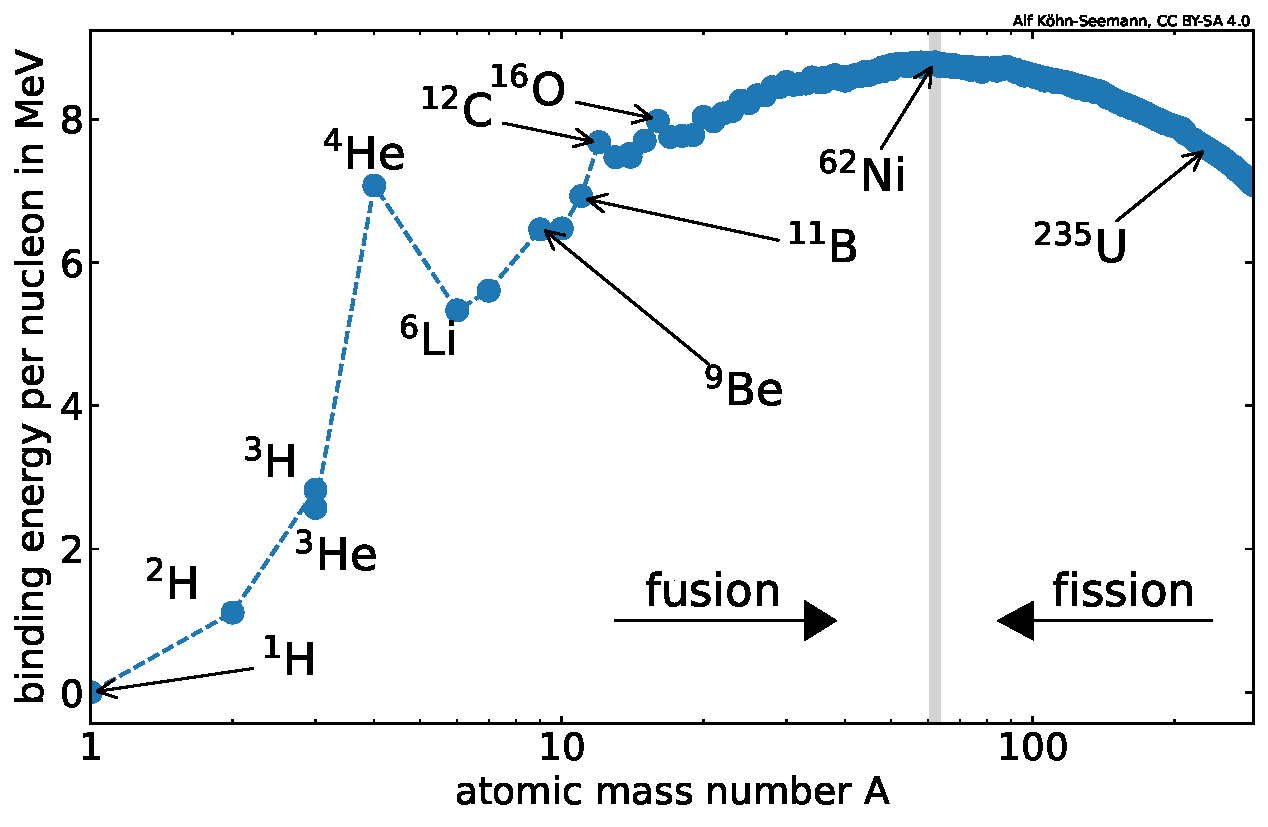
\includegraphics[width=\linewidth]{Figures/Chapter1/binding_energy_per_nucleon.pdf}
    \caption{Binding energy per nucleon \cite{kohn-seemann_alfkoehnfusion_plots_2021}.}
    \labfig{binding energy per nucleon}
\end{figure}

Nuclei are positively charged.
To be able to fuse, they must overcome the Coulomb barrier induced by the electromagnetic repulsion (see \reffig{potential energy diagram fusion}).
This Coulomb barrier increases with the charge of the nuclei (i.e.\ the number of protons).
This means that the nuclei must collide with a high enough velocity.
At the atomistic scale, the velocity $v_\mathrm{th}$ is a function of temperature (see \refeq{thermal velocity}).
This is one of the reasons why the probability of a fusion reaction (called cross-section) is temperature dependent.

\begin{equation}
    v_\mathrm{th} = \sqrt{\frac{k_B T}{m}}
    \labeq{thermal velocity}
\end{equation}
where $k_B = \SI{1.3806e-23}{m^2.s^{-2}.kg.K^{-1}}$ is the Boltzmann constant, $T$ is the nucleus temperature in \si{K} and $m$ is the nucleus mass in \si{kg}.


\begin{figure} [h]
    \centering
    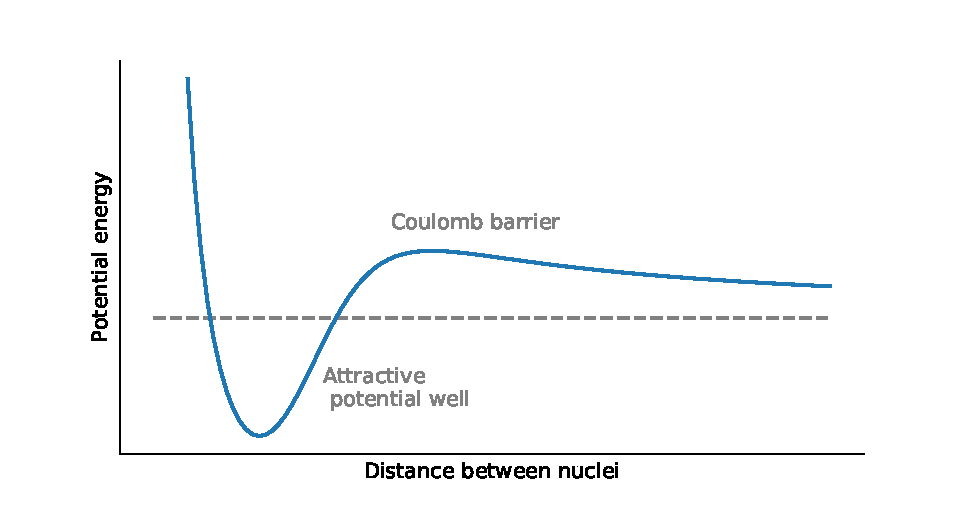
\includegraphics[width=\linewidth]{Figures/Chapter1/potential_energy.pdf}
    \caption{Evolution of the potential energy of two nuclei with their relative distance. Reproduced from \cite{mccracken_fusion_2013}.}
    \labfig{potential energy diagram fusion}
\end{figure}

Hydrogen, as the lightest element, has the lowest fusion temperature.
It is also the most abundant element on Earth (although bond to other elements).
Depending on which hydrogen \gls{isotope} is used, different fusion reactions are possible (see Equations \refeq{fusion reactions}) \cite{forrest_fendl-3_2012}.

\begin{subequations}
    \begin{equation}
         \ce{^2H + ^2H -> ^3H (\SI{1.01}{MeV}) + n (\SI{3.02}{MeV})}
    \end{equation}
    \begin{equation}
        \ce{^2H + ^2H -> ^3He (\SI{0.82}{MeV}) + n (\SI{2.45}{MeV})}
    \end{equation}
    \begin{equation}
        \ce{^2H + ^3H -> ^4He (\SI{3.5}{MeV}) + n (\SI{14.1}{MeV})}
    \end{equation}
    \begin{equation}
        \ce{^2H + ^3He -> ^4He (\SI{3.6}{MeV}) + p (\SI{14.7}{MeV})}
    \end{equation}
    \labeq{fusion reactions}
\end{subequations}

\begin{figure} [h]
    \centering
    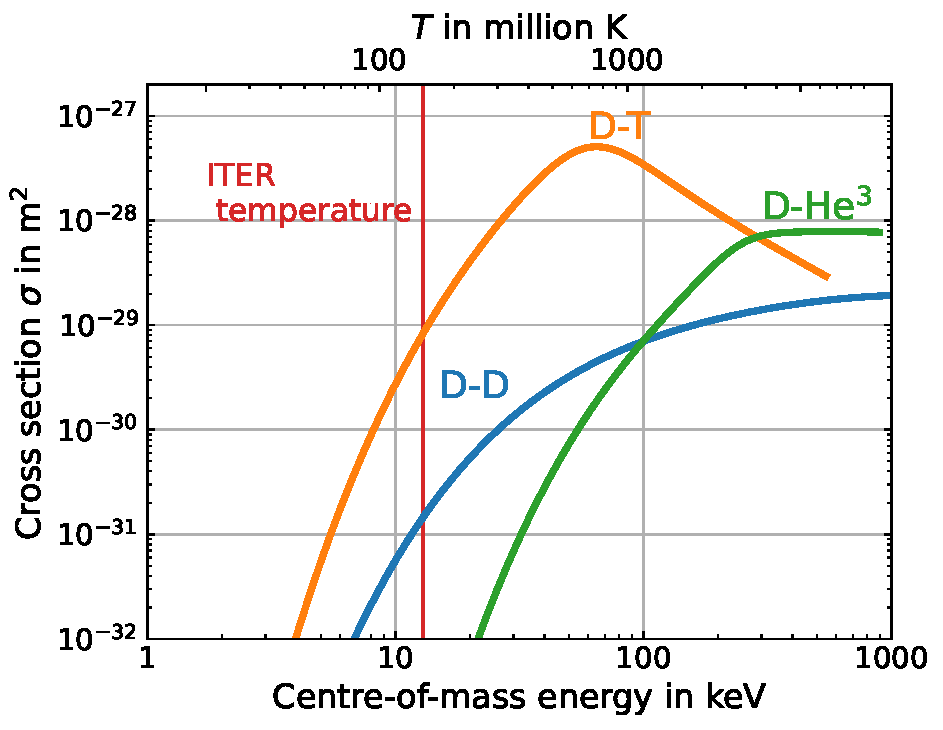
\includegraphics[width=\linewidth]{Figures/Chapter1/cross_sections_vs_temperature__Bosch.pdf}
    \caption{Fusion cross sections \cite{forrest_fendl-3_2012}.}
    \labfig{fusion cross sections}
\end{figure}
Each of these reactions has a different cross-section (measure of the reaction probability).
The \gls{D}-\gls{T} reaction is the one with the highest cross-section at `low` temperature (see \reffig{fusion cross sections}).
This is the reason why this reaction has been the focus of nuclear fusion for decades.
More recently, private companies have started experimenting with more exotic reactions like proton-boron (TAE Technologies) or $^2$H-$^3$He (Helion Energy).

% \begin{figure} [h]
%     \centering
%     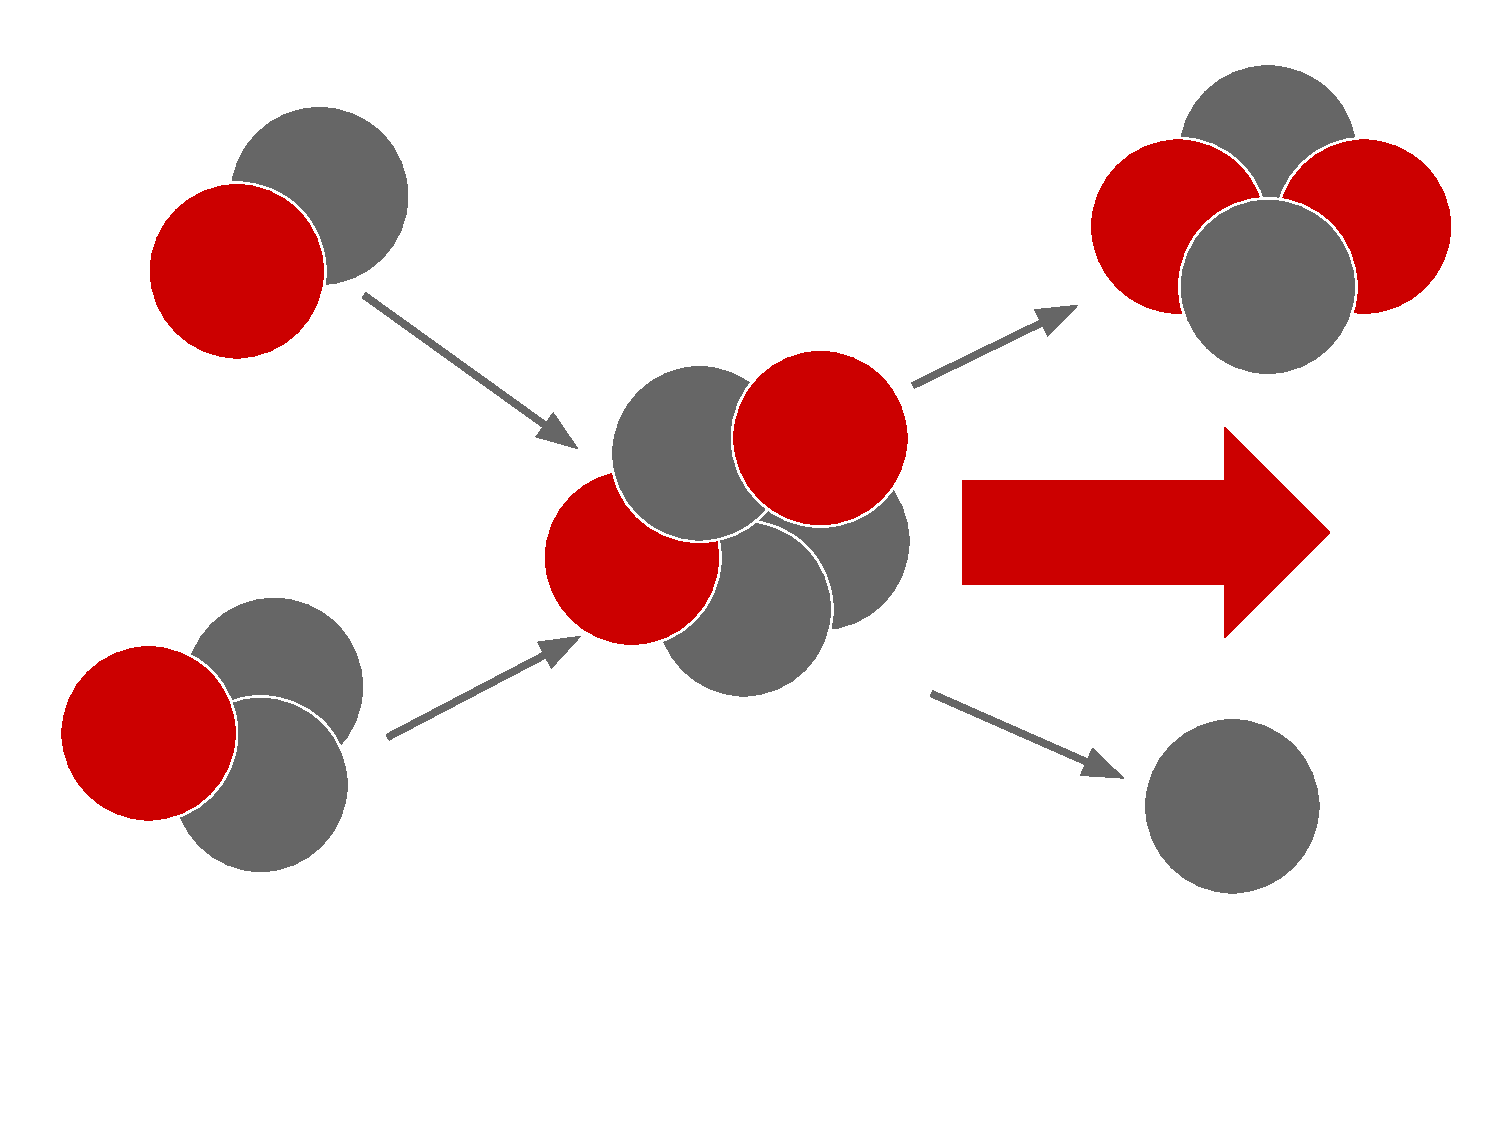
\includegraphics[width=\linewidth]{Figures/Chapter1/nuc_fus.pdf}
%     \caption{DT reaction}
% \end{figure}

\section{Tokamaks: how to bottle a star}

\subsection{Technology \cite{mccracken_fusion_2013}}
As explained above, for fusion to occur, the fuel must be heated up to millions of degrees.
A these temperatures, the DT gas becomes a \gls{plasma} where electrons are teared out from the nuclei.
The principle of magnetic confinement reactors is to trap the electrically charged particles in a magnetic cage.
The electrons and ions then gyrate around the magnetic field lines and the Larmor radius of the gyration is given by:
\begin{equation}
    R =  \frac{\sqrt{2 m T}}{e B}
\end{equation}
where $m$ is the mass of the particle, $T$ its temperature, $e$ its charge and $B$ the magnetic field.
In a hot \gls{plasma} (\SI{10}{keV}) with a strong magnetic field of \SI{3}{T}, the Larmor radius of ions is $\approx \SI{1}{mm}$, which is much smaller compared to the size of a reactor.
The Larmor radius of an electron is orders of magnitude smaller due to its lower mass.
Straight magnetic lines can therefore confine charged particles in the direction perpendicular to the field lines.
However, the particles are not confined in the parrallel direction.

This issue can be solved by closing the field lines, forming a torus-shaped magnetic field.
However, this configuration poses another problem: bending the field lines creates a magnetic field gradient in the radial direction.
This magnetic field gradient and the centrifugal force cause the particles to drift upwards (or downwards depending on their charge).
Due to this drift, the particles end up escaping the magnetic confinement until they touch the walls of the chamber and neutralise (making it impossible for them to fuse).

Two options exist to compensate this drift.
The first is to add a poloidal component to the magnetic field and twist the magnetic lines.
This is done by inducting a current in the \gls{plasma} thanks to a central solenoïd (see Figure~\ref{fig:tokamak magnetic field}).
This configuration is called \Gls{tokamak} which stands for `toroidalnaïa kamera s magnitnymi katouchkami` (toroidal chamber with magnetic coils).

\begin{figure}[h]
    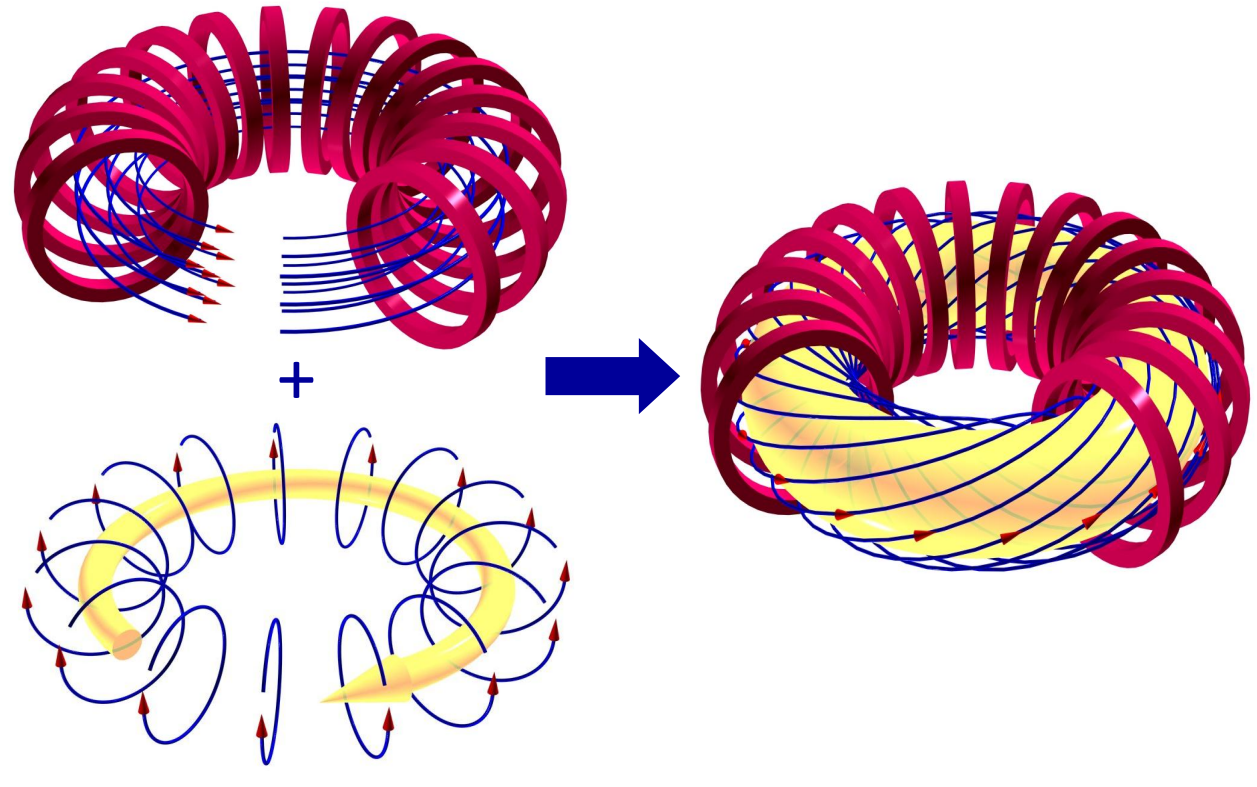
\includegraphics[width=\linewidth]{Figures/Chapter1/tokamak_magnetic_fields.png}
    \caption{Magnetic field lines in a tokamak. Contribution of the toroidal and poloidal components.}
    \label{fig:tokamak magnetic field}
\end{figure}

The second option is to twist the magnetic field by twisting the toroidal coils themselves.
This configuration is called a \gls{stellarator} and has the advantage of not having an induced current and is therefore inherently steady-state.
The \gls{tokamak}, on the other hand, is a pulsed device.
This is because the central solenoid has a limited capacity.
The main drawback of the the \gls{stellarator} is the complexity of the coils.
Since each coil has a unique shape, the cost of manufacturing such a reactor is higher than \glspl{tokamak} for which coils can be manufactured in series.

\subsection{Triple product}
The power balance in a fusion reactor is given by \cite{mccracken_fusion_2013}:
\begin{equation}
    \frac{\partial W}{\partial t} = P_\mathrm{fusion} + P_\mathrm{heating} - P_\mathrm{losses}
    \labeq{plasma energy balance}
\end{equation}
$W$ is the thermal energy density stored in the \gls{plasma} and can be expressed in \si{J.m^{-3}} by:
\begin{equation}
    W = 3 n T
\end{equation}
where $n$ is the \gls{plasma} density in \si{m^{-3}} and $T$ is the \gls{plasma} temperature in \si{J}.
$P_\mathrm{fusion}$, expressed in \si{W.m^{-3}}, is the power density generated from fusion reactions themselves and can be expressed by:
\begin{equation}
    P_\mathrm{fusion} = n_D n_T \left\langle \sigma \right\rangle E
\end{equation}
where $n_D$ and $n_T$ are the densities in \si{m^{-3}} of deuterium and tritium respectively, $\left\langle \sigma \right\rangle$ is the DT reactivity in \si{m^3.s^{-1}} and $E$ is the energy of the fusion reaction in \si{J}.
Because the neutrons have little interaction with the \gls{plasma}, $E \approx E_\alpha = \SI{3.56}{MeV}$.
Moreover, assuming a 50\%-50\% mixture of deuterium and tritium, $n_D = n_T = \frac{1}{2} n$.
The fusion power can therefore be written as:
\begin{equation}
    P_\mathrm{fusion} = \frac{1}{4} n^2 \left\langle \sigma \right\rangle E_\alpha
\end{equation}

The amplification factor $Q$ defines the ratio of the fusion power by the heating power.
The heating power $P_\mathrm{heating}$ is therefore written as:
\begin{equation}
    P_\mathrm{heating} = \frac{P_\mathrm{fusion}}{Q}
\end{equation}

Finally, $P_\mathrm{losses}$ is the rate at which the \gls{plasma} loses energy, either by losing mass (particles escaping the magnetic cage) or by radiation.
It is characterised by an energy confinement time $\tau_E$ and can be expressed as:
\begin{equation}
    P_\mathrm{losses} = \frac{W}{\tau_E} = \frac{3 n T}{\tau_E}
\end{equation}

Assuming energy equilibrium (i.e.\ $\frac{\partial W}{\partial t} = 0$), \refeq{plasma energy balance} can therefore be written as:
\begin{align}
    P_\mathrm{losses} &= P_\mathrm{fusion} + P_\mathrm{heating} \\
    \Leftrightarrow \frac{3 n T}{\tau_E} &= \frac{1}{4} n^2 \left\langle \sigma \right\rangle E_\alpha + \frac{P_\mathrm{fusion}}{Q}
\end{align}

Re-arranging the terms, one can obtain:
\begin{equation}
    n T \tau_E = \frac{12 T^2}{\left\langle \sigma \right\rangle E_\alpha} \cdot \frac{1}{1 + \frac{1}{Q}}
    \labeq{triple product}
\end{equation}

$n T \tau_E$ is known as the \textit{triple product}, a figure of merit describing the performance of a fusion reactor.
\refeq{triple product} gives the triple-product required to achieve a given amplification factor $Q$ at a given temperature $T$.

When $P_\mathrm{heating}$ approaches zero (i.e.\ the auxilliary heating systems are shut down), the amplification factor $Q$ approaches $\infty$.
Therefore:
\begin{equation}
    n T \tau_E \rightarrow \frac{12 T^2}{\left\langle \sigma \right\rangle E_\alpha}
    \labeq{triple product infinity}
\end{equation}

The quantity $T^2/\langle \sigma \rangle$ has a minimum around $T=\SI{14}{keV}$.
Furthermore, when $\SI{10}{keV} < T < \SI{20}{keV}$, the DT reactivity can be approximated by $\langle \sigma \rangle \approx 1.1 \times 10^{-24} T^2$.

\refeq{triple product infinity} can therefore be written as:
\begin{equation}
    n T \tau_E \geq \SI{3e21}{keV.s.m^{-3}}
\end{equation}

This is known as the Lawson criterion, which needs to be satisfied in order to reach \textit{ignition} ($Q = \infty$).


Fusion devices can therefore be classified into three categories.
Stars like our Sun have very high confinement times and densities while remaining at relatively low temperatures (the sun core is at \SI{1.2}{keV}).
Magnetic confinement devices (\glspl{tokamak}, \glspl{stellarator}, etc.) exhibit temperatures orders of magnitude higher than stars but have confinement times of the order of $\sim \SI{1}{s}$.
A third way of achieving fusion is to heat and compress a target of fuel with either lasers (\acrshort{nif} \sidecite{zylstra_burning_2022}, Laser Mega Joule \sidecite{miquel_laser_2016}), pistons (General Fusion) or by smashing it at high speed with a projectile (First Light Fusion).
These devices, known as \textit{inertial fusion devices}, exhibit extremely high densities ($\sim \SI{e31}{m^{-3}}$) but short confinement times ($\sim \SI{e-11}{s}$).
 
So far, no fusion device has been able to even reach \textit{break-even} ($Q = 1$) (see \reffig{triple product vs T}).
The record of $Q = 0.68$ by the European \gls{tokamak} \gls{jet} and was performed in 1997 \sidecite{mailloux_overview_2022}.
The objective of the \acrshort{iter} \gls{tokamak}, currently under construction in France, is to demonstrate an amplification factor of $Q=10$ over \SI{400}{s} \sidecite{casper_development_2013}. 
Note that \acrshort{iter} will not produce any electricity as this will be the role of a future fusion reactor: DEMO \sidecite{federici_overview_2014}.
Other designs aim at demonstrating \gls{plasma} gain (i.e.\ $Q > 1$) sooner than \acrshort{iter} and at a smaller scale (see \reffig{comparison reactors}).
This is the case of \acrshort{sparc} and \acrshort{arc} developed by Commonwealth Fusion Systems and MIT \sidecite{sorbom_arc_2015,creely_overview_2020} or \acrshort{step} designed by the \gls{ukaea} \sidecite{wilson_steppathway_2020}.

\begin{figure}
    \centering
    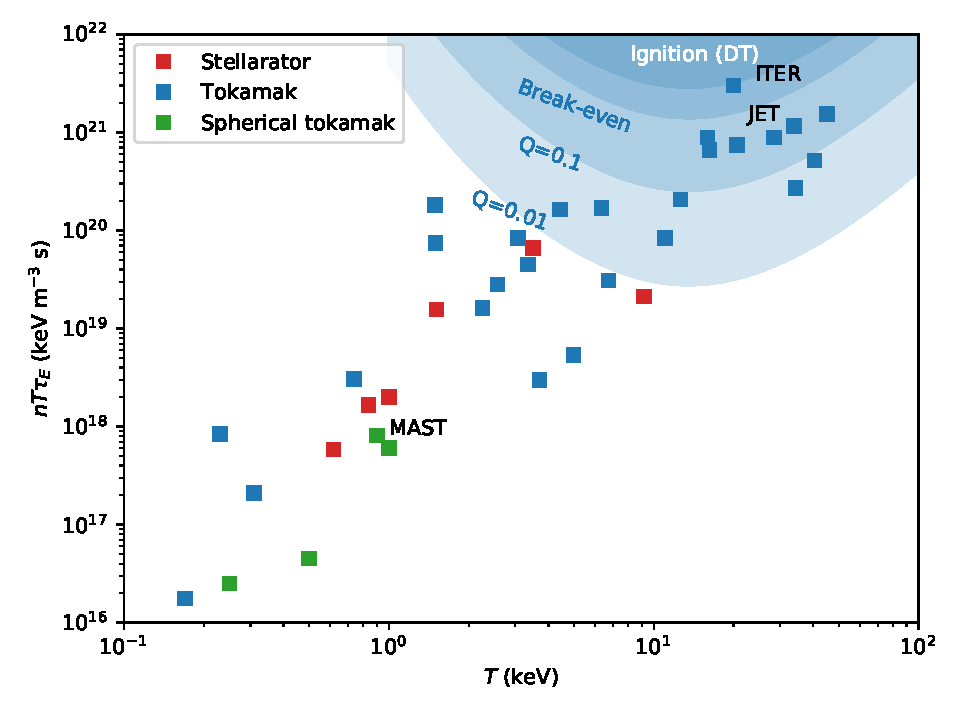
\includegraphics[width=\linewidth]{Figures/Chapter1/triple_product_vs_T.pdf}
    \caption{Triple product. An interactive version of this plot is available at \cite{delaporte-mathurin_remdelaportemathurinfusion-world_2022}.}
    \labfig{triple product vs T}
\end{figure}

\begin{figure}
    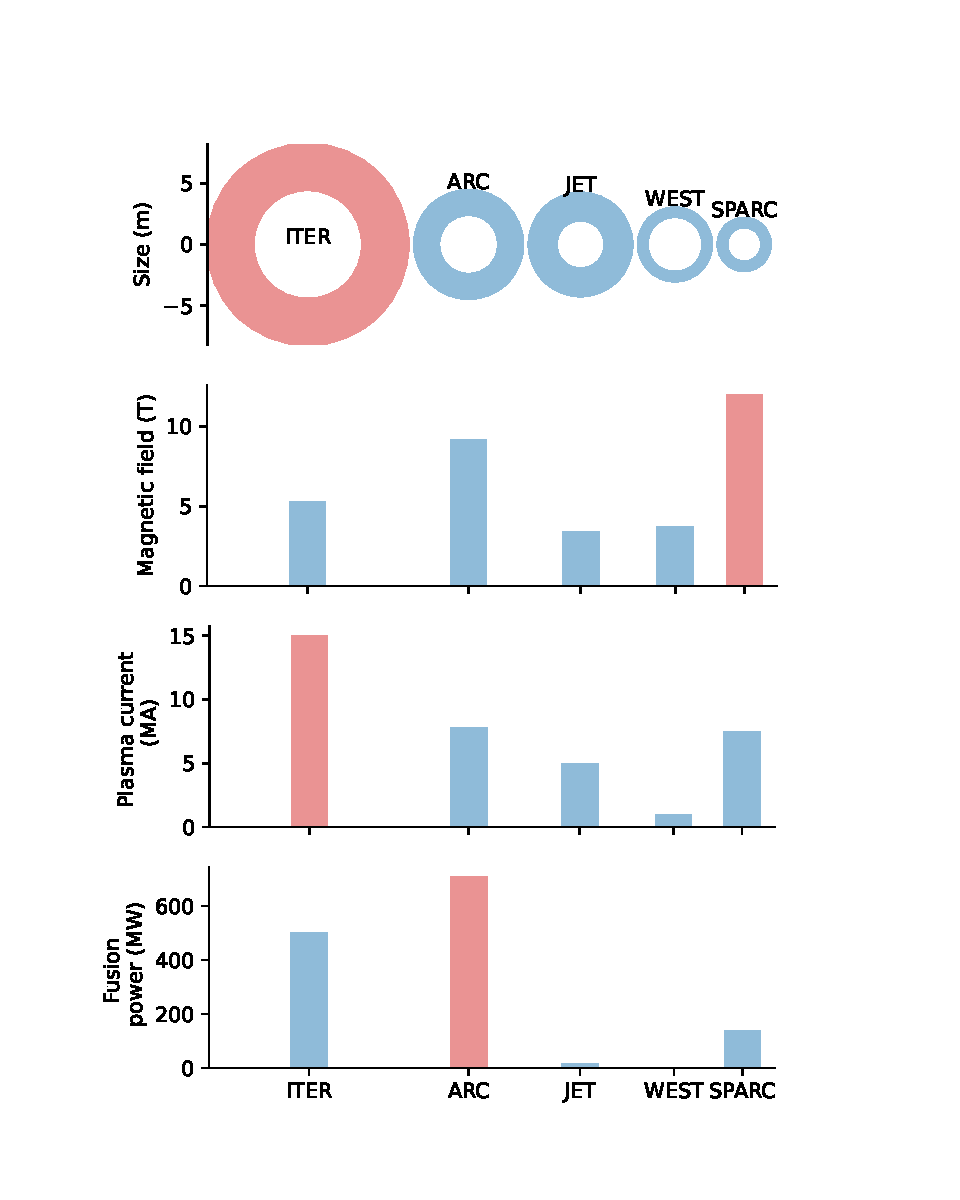
\includegraphics[width=0.9\linewidth]{Figures/Chapter1/comparison_reactors.pdf}
    \caption{Comparison of the tokamaks \acrshort{iter} , JET, ARC, WEST and SPARC. Data from \cite{delaporte-mathurin_remdelaportemathurinfusion-world_2022}.}
    \labfig{comparison reactors}
\end{figure}

\subsection{Plasma-facing materials}

The walls of a fusion reactor are exposed to intense heat and particle fluxes.
The choice of \glspl{pfm} is therefore crucial.

An appropriate \gls{pfm} must have good thermal properties to withstand the extreme heat fluxes.
A high thermal conductivity is required as well as a very high melting point to enhance heat exhaust but also minimise the impact of arcing (material release from erosion) \sidecite{ivanova_plasma-facing_2012, mccracken_review_1980}.
The material must also resist to thermal chocs encountered during short \gls{plasma} discharges or transient events in the \gls{plasma} \sidecite{van_den_kerkhof_impact_2021}.

In order to maximise the components lifespan, \glspl{pfm} must resist erosion.
This is even more important when the eroded particle reduce \gls{plasma} performances by making it radiate and cool down.

The choice of a \gls{pfm} is also important from the nuclear safety point of view.
First, the quantity of tritium retained in the materials need to be minimised (this point will be detailed in Section \ref{the tritium issue}).
Second, neutron activation of the material can increase the quantity of radioactive waste and must be minimised.

One of the first \gls{pfm} was \gls{cfc} \sidecite{linke_challenges_2019}.
\gls{cfc} had the great advantage of not melting and withstand very high heat fluxes.
Using \gls{cfc} also increased the \gls{plasma} performances greatly \sidecite{federici_plasma-material_2001}.
Unfortunately, graphite being porous, hydrogen (and therefore tritium) retention was high \sidecite{sugiyama_measurement_2004}.
Plus carbon can react with \gls{plasma} particles forming methane.
Methane is then deposited on locations hard to access in the reactor \gls{trapping} tritium even more.
For these two safety reasons, \gls{cfc} was replaced with tungsten or beryllium (or both).

\Gls{W} has a very high melting point (\SI{3422}{°C}) and retains less tritium \sidecite{pajuste_tritium_2021}.
However, tungsten being a high-Z element, eroded tungsten will make the \gls{plasma} radiate and cool it down.
For this reason, the \acrshort{iter} divertor will be made of tungsten but the first wall (which has a large surface area) will be made of beryllium.

\subsection{Divertor}\labsec{divertor section}

In a fusion reactor, heat and particles (fusion ashes) need to be extracted.
In most \glspl{tokamak}, the escaping \gls{plasma} is diverted towards a dedicated component that is heat-resistant.
Such a configuration is called a \emph{\gls{divertor}} configuration.
The X-divertor is a common configuration (used in \acrshort{west}, \acrshort{jet}, \acrshort{iter}) but more advanced configurations exist such as the Super-X \gls{divertor} (\acrshort{mast-u}) \sidecite{havlickova_effect_2015}, X-Point Target (\acrshort{sparc}) \sidecite{rodriguez-fernandez_overview_2022, kuang_divertor_2020} or the Snowflake configurations \sidecite{ryutov_snowflake_2015}.

\begin{figure} [h]
    \centering
    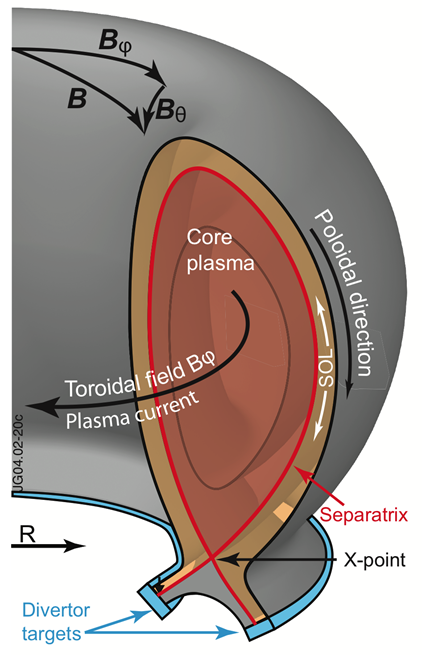
\includegraphics[width=0.5\linewidth]{Figures/Chapter1/sketch_divertor.png}
    \caption{Sketch of the tokamak divertor configuration (source: EFDA-JET).}
    \labfig{divertor diagram}
\end{figure}

In a \gls{divertor} configuration, the intersection between the magnetic field lines and the targets are called \emph{\glspl{strike point}}.
The X-divertor has two \glspl{strike point} on the inner and outer targets (see \reffig{divertor diagram}).
At these \glspl{strike point}, the targets will experience very intense heat and particle fluxes (see \reffig{divertor exposure conditions}).

\begin{figure} [h]
    \centering
    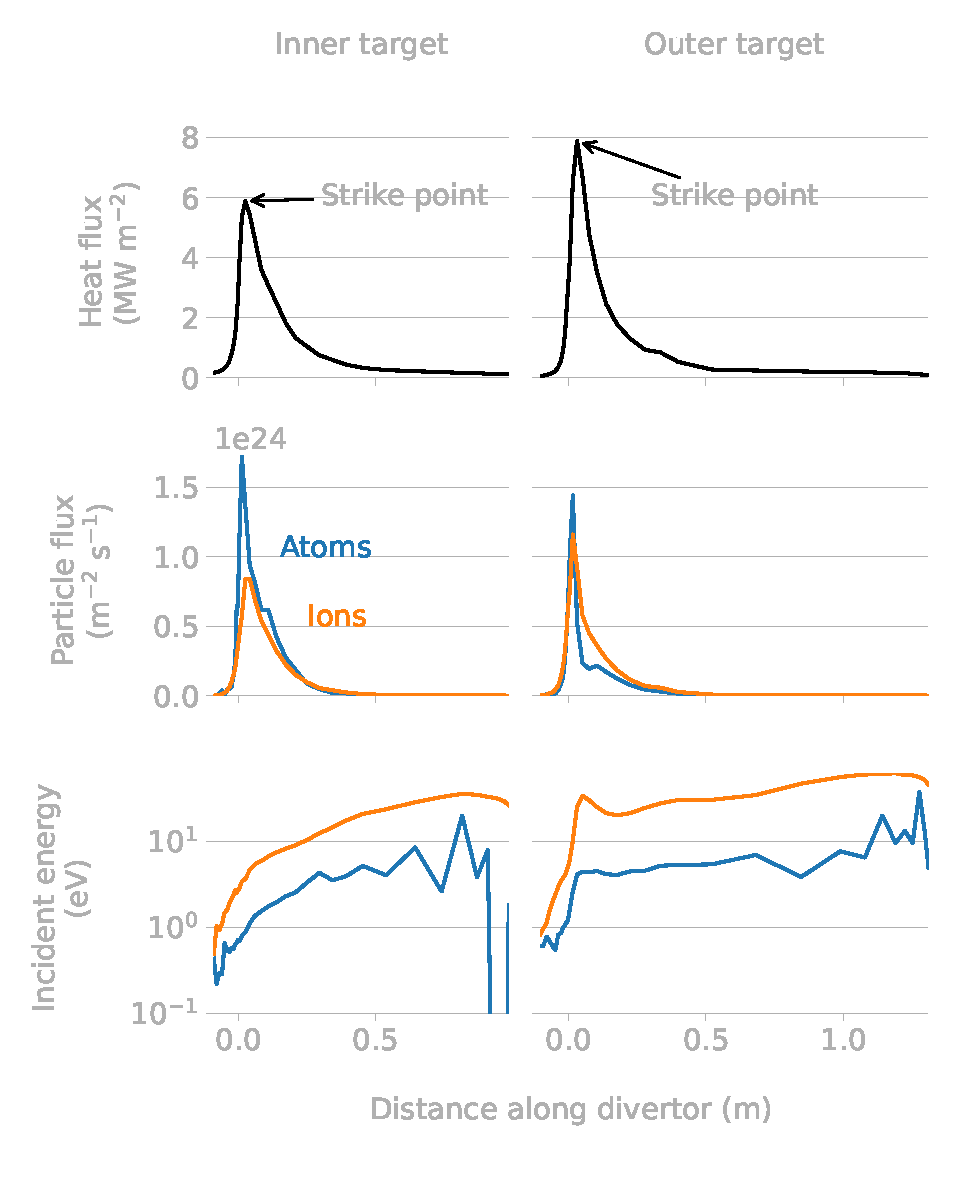
\includegraphics[width=\linewidth]{Figures/Chapter1/divertor_exposure_conditions.pdf}
    \caption{Heat flux, particle flux and particle energy along the \acrshort{iter} divertor computed by SOLPS (shot \#122399) \cite{pitts_physics_2019}.}
    \labfig{divertor exposure conditions}
\end{figure}

The \acrshort{iter} divertor will be composed of 54 cassettes (see \reffig{monoblock to divertor}).
Each cassette is made of two targets - the \gls{ivt} and \gls{ovt} - , a dome and two reflector plates.
The inner and outer \glspl{strike point} (respectively \acrshort{isp} and \acrshort{osp}) will be located on the \gls{ivt} and the \gls{ovt}.
A prototype of the \gls{ivt} is shown on \reffig{inner target photo}.
These elements are themselves made of rows, called \glspl{pfuLabel}, of small unit bricks of a few dozens of milimetres called \glspl{monoblock}.
In \acrshort{iter} , the \gls{ivt} has 16 \glspl{pfuLabel} and the \gls{ovt} has 22 \glspl{pfuLabel}.
\Glspl{monoblock} are typically made of a tungsten substrate with a cooling pipe running through.
This cooling channel is necessary to keep the component's temperature below its operating limit and exhaust heat.

Several \gls{monoblock} designs are currently studied for DEMO with varying dimensions, different materials for the cooling pipe or the interlayer, etc \sidecite{vizvary_european_2020, huang_tungsten_2016, hirai_use_2016, domptail_design_2020}.
The main candidate is the ITER-like design, the type of \gls{monoblock} that will be used in \acrshort{iter} \cite{hirai_use_2016}.
This design has a tunsgten substrate with a CuCrZr cooling pipe and a Cu interlayer for compliance.
In \acrshort{iter}, \glspl{monoblock} will be \SI{12}{mm}-thick whereas they will be thiner (\SI{4}{mm}) in DEMO \sidecite{you_european_2018}.

\begin{figure*}
    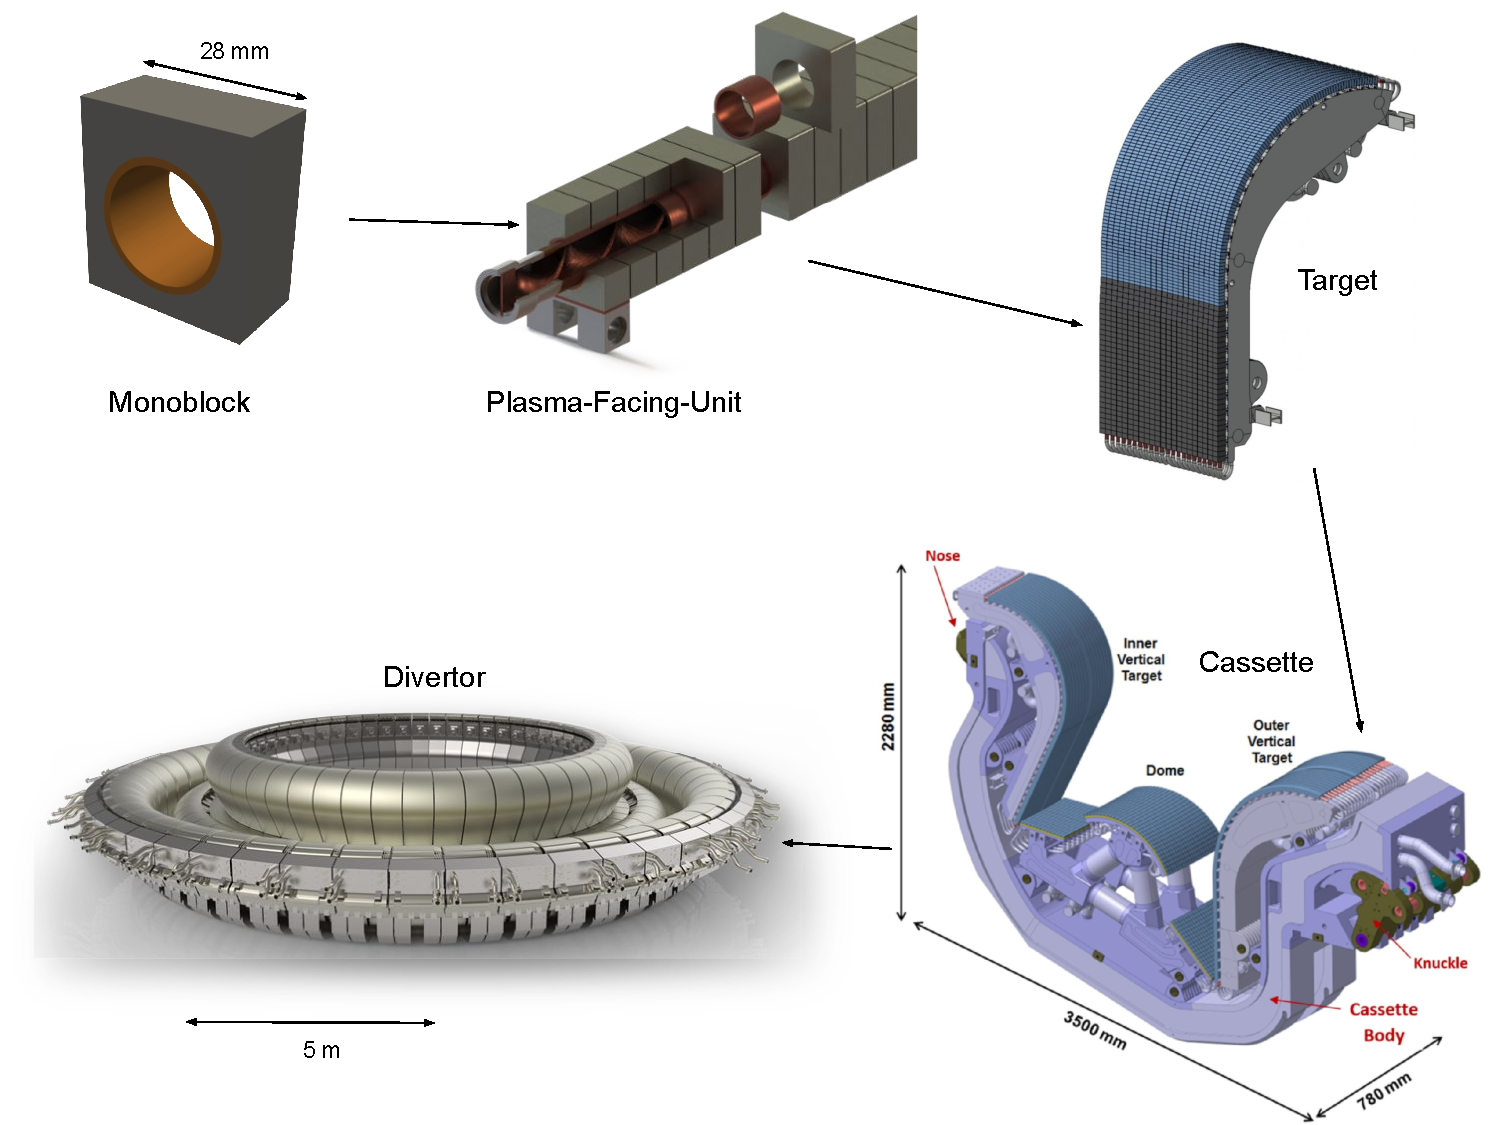
\includegraphics[width=\linewidth]{Figures/Chapter1/monoblock_to_divertor.pdf}
    \caption{Structure of the \acrshort{iter} divertor. (images: ITER Organization, \cite{guerrini_fabrication_2021}).}
    \labfig{monoblock to divertor}
\end{figure*}

\begin{figure} [h]
    \centering
    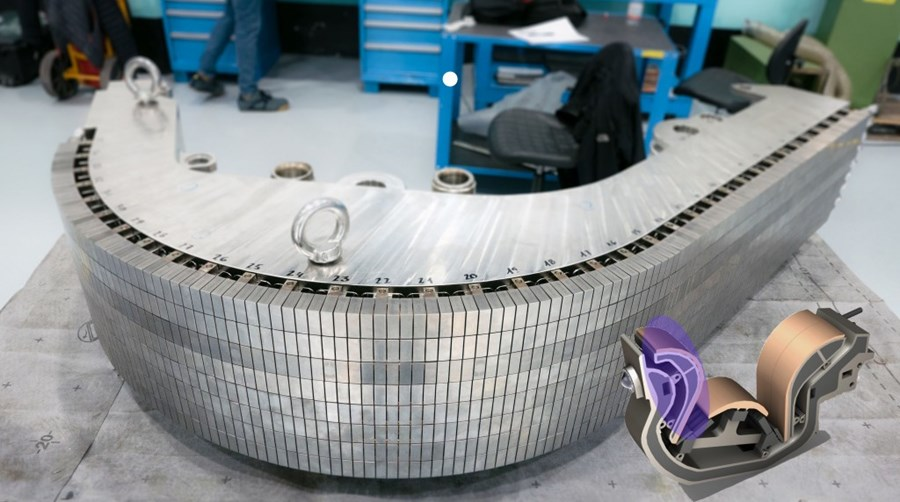
\includegraphics[width=0.8\linewidth]{Figures/Chapter1/inner_target_iter.jpg}
    \caption{Prototype of the inner vertical target (source: ITER Organization).}
    \labfig{inner target photo}
\end{figure}

Studies on ITER-like \glspl{monoblock} have demonstrated the resistance of the \gls{monoblock} design to high heat loads while investigating the effect of tungsten recrystallisation \sidecite{durif_impact_2019, durif_modelisation_2019, visca_manufacturing_2018} (see \reffig{monoblock_temperature_exp_model}).

\begin{figure} [h]
    \centering
    \begin{subfigure}[t]{0.45\linewidth}
            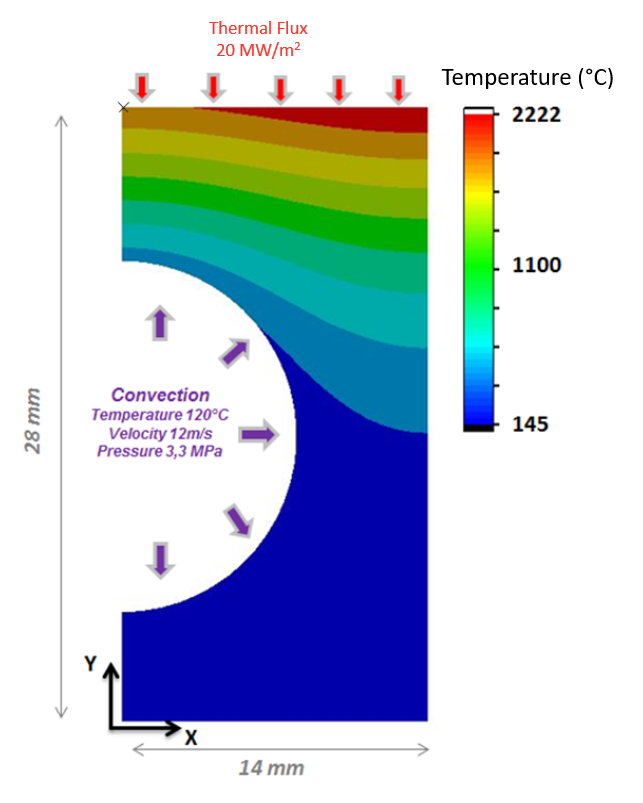
\includegraphics[width=\linewidth]{Figures/Chapter1/alan_durif_monoblock.png}
            \caption{Simulated temperature field in a monoblock at \SI{20}{MW.m ^{-2}} heat loading, water cooling at \SI{120}{\celsius}. Reproduced from \cite{durif_modelisation_2019}.}
    \end{subfigure}\hfill%%
    \begin{subfigure}[t]{0.45\linewidth}
            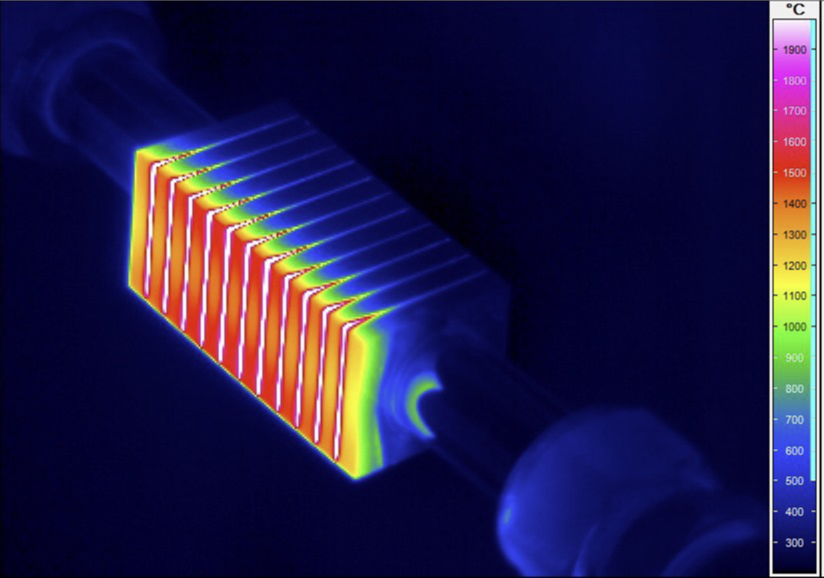
\includegraphics[width=\linewidth]{Figures/Chapter1/monoblock_experimental_temperature_field.png}
            \caption{Experimental measurement of monoblocks thermal response at \SI{20}{MW.m ^{-2}} heat loading, water cooling at \SI{130}{\celsius}. Reproduced from \cite{visca_manufacturing_2018}.}
    \end{subfigure}
    \caption{Thermal response of ITER-like monoblocks.}
    \labfig{monoblock_temperature_exp_model}
\end{figure}

\section{The tritium issue} \label{the tritium issue}

Tritium is a radioactive \gls{isotope} of hydrogen with a half-life is approximately 12 years \sidecite{jordan_half-life_1967}.
It decays into $^3$He emitting a beta particle (see \refeq{tritium decay}).

\begin{equation}
    \ce{^3H -> ^3He + e^- (\SI{0.018590}{MeV})}
    \labeq{tritium decay}
\end{equation}

This is an issue for both the fuel supply chain and nuclear safety.

\subsection{Breeding}
Due to its radioactive nature, tritium is very rare on Earth.
The current reserve of tritium in the world is a few dozens of kilograms.
It is naturally produced by interaction of comsic rays with the nitrogen in the atmosphere (\SI{0.2}{kg} per year).
Tritium is however produced in larger quantities in fission \gls{candu} reactors as a by-product (\SI{130}{g} per year per \gls{candu} reactor \sidecite{ni_tritium_2013}).

\acrshort{iter} itself will consume around \SI{18}{kg} of tritium over the duration of its operation \sidecite{glugla_iter_2007}, which represent a yearly consumption of \SI{0.9}{kg} for a 20-year lifetime.
A \SI{800}{MWe} DEMO-type commercial fusion reactor would burn around \SI{300}{g} of tritium per day ($\approx \SI{100}{kg}$ a year).

For all these reasons, tritium must be produced on-site in large quantities for a fusion economy to be possible.

To this end, the neutrons of the DT fusion reactions will be harnessed in a component containing \gls{Li} surrounding the \gls{plasma} called the \emph{\gls{breeding blanket}} (see \reffig{blanket_shimwell}).


\begin{figure}
    \centering
    \begin{subfigure}{0.45\linewidth}
        \includegraphics{Figures/Chapter1/blanket_shimwell_top_view.png}
        \caption{View from above.}
    \end{subfigure}%
    \qquad
    \begin{subfigure}{0.45\linewidth}
        \includegraphics{Figures/Chapter1/blanket_shimwell_side_view.png}
        \caption{Side view.}
    \end{subfigure}
    \caption{DEMO model showing HCLL blankets \cruleme[lithiumgreen]{0.3cm}{0.3cm}, plasma \cruleme[plasmapink]{0.3cm}{0.3cm}, magnets \cruleme[magnetred]{0.3cm}{0.3cm}, and structural steel \cruleme[steelgray]{0.3cm}{0.3cm}. Reproduced from \cite{shimwell_multiphysics_2019}.}
    \labfig{blanket_shimwell}
\end{figure}

Depending on the \gls{Li} \gls{isotope}, two reactions can occur:

\begin{align}
    \text{n} + \text{\textsuperscript{6}Li}  \ \ &\xrightarrow{} \ \ \text{\textsuperscript{3}H} + \alpha + \SI{4.8}{MeV}\\
    \text{n} + \text{\textsuperscript{7}Li}  \ \ &\xrightarrow{} \ \ \text{\textsuperscript{3}H} + \alpha + \text{n}' - \SI{2.5}{MeV} 
\end{align}

Several \glspl{breeding blanket} designs have been proposed divided in three main categories: ceramic concepts, liquid metal concepts, and molten-salts concepts.
All designs differ in the choice of tritium breeder, coolant and geometry.

The european candidates for \glspl{breeding blanket} in DEMO are the \gls{wcll} \sidecite{aubert_design_2020, del_nevo_recent_2019}, the \gls{hcpb} \sidecite{hernandez_overview_2018, hernandez_new_2017,pereslavtsev_neutronic_2017}, the \gls{hcll} \sidecite{aubert_status_2018,jaboulay_nuclear_2017} and the \gls{dcll} \sidecite{urgorri_tritium_2017, palermo_neutronic_2015} \sidecite{federici_overview_2019}.

The \gls{tbr} is defined by the number of tritium atoms produced by generated neutrons.
In order to ensure tritium self-sufficiency, the \gls{tbr} of the blanket must be greater than or equal to one \sidecite{abdou_blanketfirst_2015}.
A \gls{tbr} greater than one can only be obtained by neutron multiplication with lead or beryllium.

Moreover, the \gls{tbr} must account for:
\begin{itemize}
    \item losses via \gls{permeation}, \gls{trapping}, radioactive decay (5\% per year)
    \item safety reserve in case of interruption of the fuel cycle
    \item supply of new reactors, also called the \emph{\gls{startup inventory}}
\end{itemize}

The \gls{tbr} target in conventional power plants is around 1.05 \sidecite{shimwell_multiphysics_2019}.
Though this would achieve self-sufficiency, it is not be enough to sustain the development of a fusion energy market.

% The desired doubling time of fusion power plants will drive this last point \sidecite{bockhoff_tritium_1983}.
The evolution of the maximum fusion power on the grid $P_\mathrm{max}$ can be expressed as:

\begin{equation}
    P_\mathrm{max} = P_\mathrm{plant} \times 2^{t/\tau_2}
\end{equation}
where $\tau_2$ is the doubling time (i.e.\ the time after which a plant has doubled its initial tritium \gls{inventory}), $t$ is the time, and $P_\mathrm{plant}$ is the power of a single plant.
This expression assumes the only source of tritium is the reactors currently under operation.

Assuming $P_\mathrm{plant} = \SI{1}{GW}$, with a doubling time $\tau_2 = \SI{2}{years}$, it will take \SI{20}{years} to produce \SI{1}{TW} of fusion electricity on the grid (see \reffig{fusion power doubling time}).
This time reaches \SI{50}{years} with a doubling time of \SI{5}{years}.

\begin{figure}
    \centering
    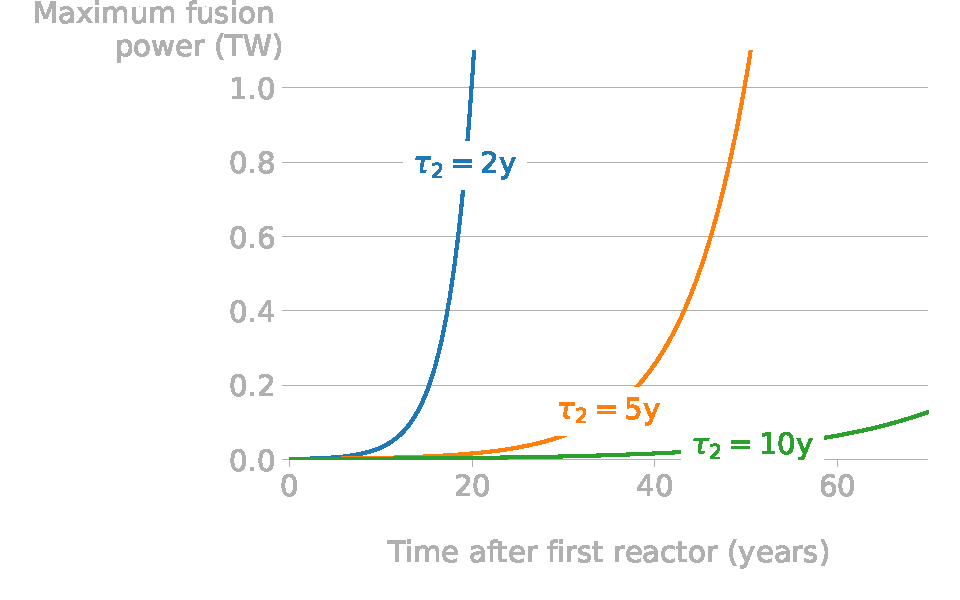
\includegraphics[width=0.8\linewidth]{Figures/Chapter1/doubling_time.pdf}
    \caption{Evolution of the maximum fusion power on the grid for different doubling times.}
    \labfig{fusion power doubling time}
\end{figure}

For fusion power plants to achieve a doubling time $\tau_2 \leq \SI{3}{years}$ (doubling times in power industry are typically \SI{5}{years}), the \gls{tbr} must be greater than 1.15 \sidecite{abdou_physics_2020}.
Other key parameters influence the required \gls{tbr} (for a given doubling time) like the tritium burn-up fraction, the fueling efficiency, the plant availability factor...

Tritium transport in \glspl{breeding blanket} is crucial as trapped tritium in solid parts would increase the \gls{startup inventory}.
For a given doubling time, a higher \gls{startup inventory} means a higher \gls{tbr} requirement.
The blanket \gls{inventory} in the solid parts can be reduced by (1) reducing the amount of solid components (this will also increase the \gls{tbr} \cite{shimwell_multiphysics_2019}) (2) designing permeation barriers \sidecite{utili_design_2022}.
% Understanding hydrogen transport in these components is therefore crucial for the future of nuclear fusion technology.

\subsection{Safety}
Tritium is also an issue in terms of nuclear safety.
As a radioactive \gls{isotope}, its ingestion - in the form of tritiated water HTO - is a health hazard.
Its biological half-life (i.e.\ once ingested by humans) is around 10 days - which can be considered as low toxicity \sidecite{bridges_review_2007,janssens_emerging_2007}.
Tritium's half-life once incorporated in organic compounds increases to 40 days and is associated with a higher toxicity \cite{bridges_review_2007}.
To put tritium toxicity in perspective, it has been estimated that drinking \SI{2}{L} of water with the highest permissible level of tritium contamination (\SI{10000}{Bq.L^{-1}}) each day for a year results in a total radiation dose of \SI{0.1}{mSv}, which is equivalent to two weeks natural radioactivity exposure \sidecite{hyatt_radioactive_2021}.

To limit the potential environmental releases due to a loss of vacuum accident, its \gls{inventory} in fusion reactors must be limited \sidecite{honda_analyses_2000}.
In \acrshort{iter} for instance, the in-vessel \gls{inventory} of tritium is limited to \SI{1}{kg} including \SI{120}{g} retained in cryo-pumps \sidecite{roth_tritium_2008}.
This limit has been determined to avoid evacuation of population around the reactor in the event of a loss of vacuum accident.

Moreover, as tritium can migrate in materials, components that have been in contact with it are considered as tritiated waste and must be handled.
Tritium migration through complete material layers (\gls{permeation}) to the cooling tubes \sidecite{arredondo_preliminary_2021, shimada_tritium_2018} or to the atmosphere can lead to contamination of coolants and must be taken into account in the detritiation process.

Detritiation techniques are being developped to reduce the volume of tritiated waste in future fusion reactors \sidecite{liger_overview_2018}.
These techniques mainly consist in heating the tritiated samples and recovering the tritiated gas \sidecite{lefebvre_preliminary_2012} that can be reused as fuel.
Tritium minimisation techniques such as Laser Induced Desorption or \emph{baking} are also being developed to reduce the tritium \gls{inventory} during operations \sidecite{de_temmerman_efficiency_2017}.

\Gls{permeation} barriers are being studied to greatly reduce the \gls{permeation} of tritium to the coolants \sidecite{causey_416_2012,utili_design_2022,utili_development_2021}.
The idea is to coat inner and/or outer surfaces of cooling pipes with alumina-based coatings or ceramics (\textit{eg} $\mathrm{Al_2 O_3}$, $\mathrm{Cr_2 O_3}$, $\mathrm{Er_2 O_3}$).
Natural oxides are also considered for \gls{permeation} barriers.
These coatings can also act as an anti-corrosion barrier.
The use of these \gls{permeation} barriers - by definition minimising \gls{permeation} - could potentially increase materials inventories.

\section{Helium and Hydrogen in metals}

This Section summarises the main processes at stake (see \reffig{helium and hydrogen in metals sketch}) when helium and hydrogen particles interact with metals and with each other.

\begin{figure*}[h!]
    \begin{subfigure}{0.9\linewidth}
        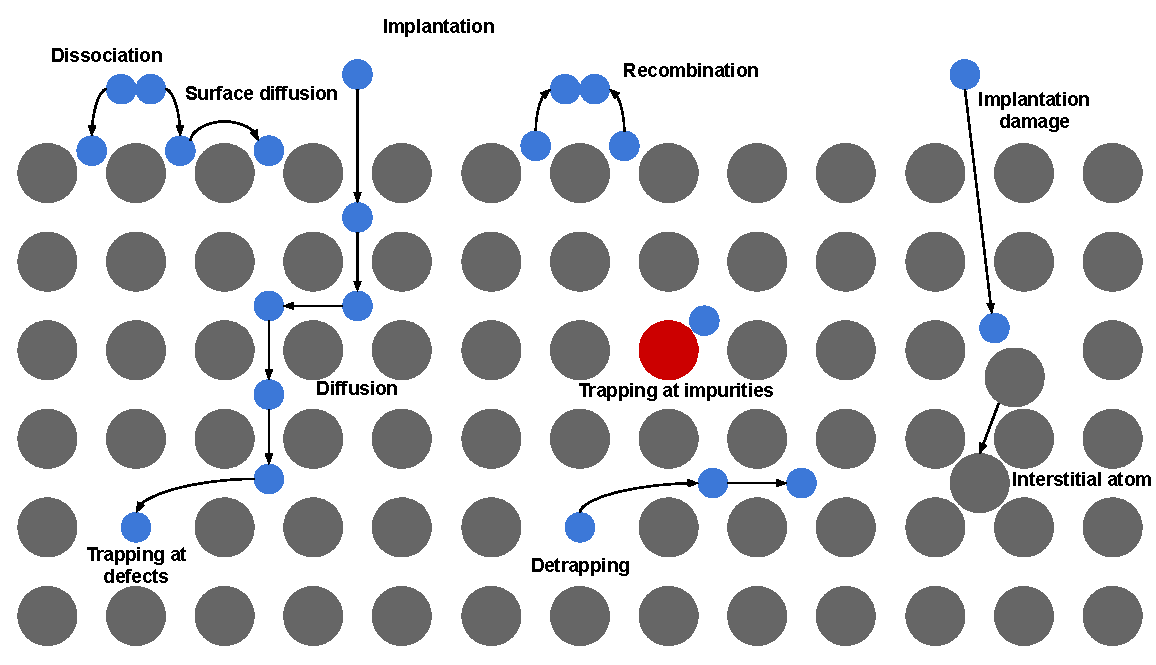
\includegraphics[width=\linewidth]{Figures/Chapter1/HI transport sketch.pdf}
        \caption{Hydrogen.}
    \end{subfigure}
    \begin{subfigure}{0.9\linewidth}
        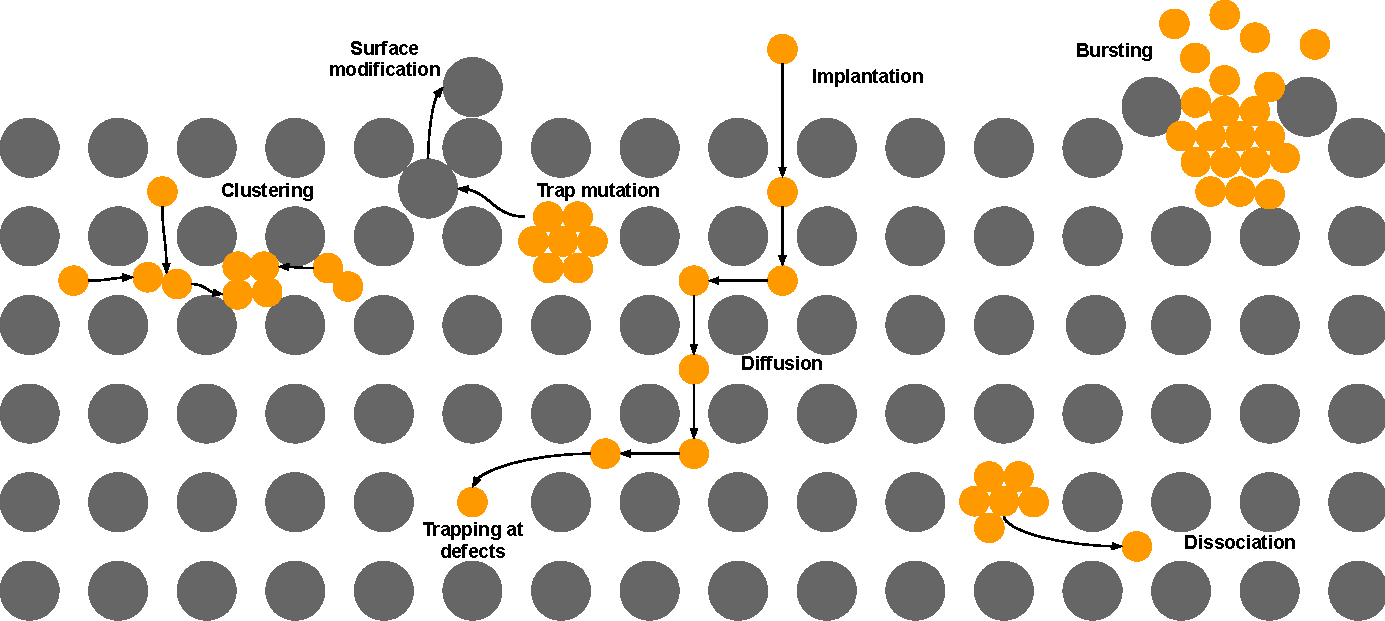
\includegraphics[width=\linewidth]{Figures/Chapter1/He transport sketch.pdf}
        \caption{Helium.}
    \end{subfigure}
    \caption{Interactions of solute species in tungsten.}
    \labfig{helium and hydrogen in metals sketch}
\end{figure*}

\subsection{Particle sources}

\subsubsection{Hydrogen}
Deuterium and tritium being the fuel of fusion reactors, the primary source of hydrogen in the \gls{divertor} is the \gls{plasma} itself.
The wall of a fusion reactor (\gls{first wall} and \gls{divertor}) is bombarded with high energy hydrogen ions.
Due to their small size, these ions can penetrate the metal \gls{lattice} and be implanted in the material.

Components are also exposed to neutral hydrogen particles either in the atomic or molecular form.
This is also the case for the \gls{divertor} region where \gls{fuel recycling} can occur \sidecite{denis_dynamic_2019, causey_hydrogen_2002}.

Tritium can also be produced by the neutron capture of helium-3 \sidecite{shimada_tritium_2017, knoll_radiation_1989} (see \refeq{he3 neutron capture reaction}).

\begin{equation}
    \ce{^3He + n -> ^1H + ^3H + \SI{0.764}{MeV}}
    \labeq{he3 neutron capture reaction}
\end{equation}

Finally, interactions of lithium with neutrons represent a major source of hydrogen in tritium \glspl{breeding blanket} \sidecite{dark_influence_2021}.

\subsubsection{Helium}\labsec{sources of helium}
Helium is the product of the fusion reaction (see \refeq{fusion reactions}).
Therefore, the wall of a fusion reactor is also bombarded with helium ions.
This is the primary source of helium in \glspl{pfm}.

Helium can also be produced in materials indirectly.
Since tritium decays into helium-3 (see \refeq{tritium decay}), regions with high tritium \gls{retention} are expected to act as a source of helium over time \cite{shimada_tritium_2017}.
Moreover, interactions of neutrons (from the fusion reactions) with metallic elements (\textit{eg} tungsten or iron) can produce helium via transmutation \sidecite{watanabe_status_2011}.
This \emph{\gls{transmutation gas}} production has been estimated using well-established neutronics simulations (Monte-Carlo simulations modelling the path of neutroncs in matter) \sidecite{gilbert_neutron-induced_2013, gilbert_integrated_2012}.
Depending on the position in the DEMO \gls{divertor}, cumulative helium production over the course of three \glspl{fpy} could reach more than \SI{400}{appm}.


\subsection{H/W \& He/W interactions}


\begin{figure} [h]
    \centering
    % \begin{subfigure}{\linewidth}
    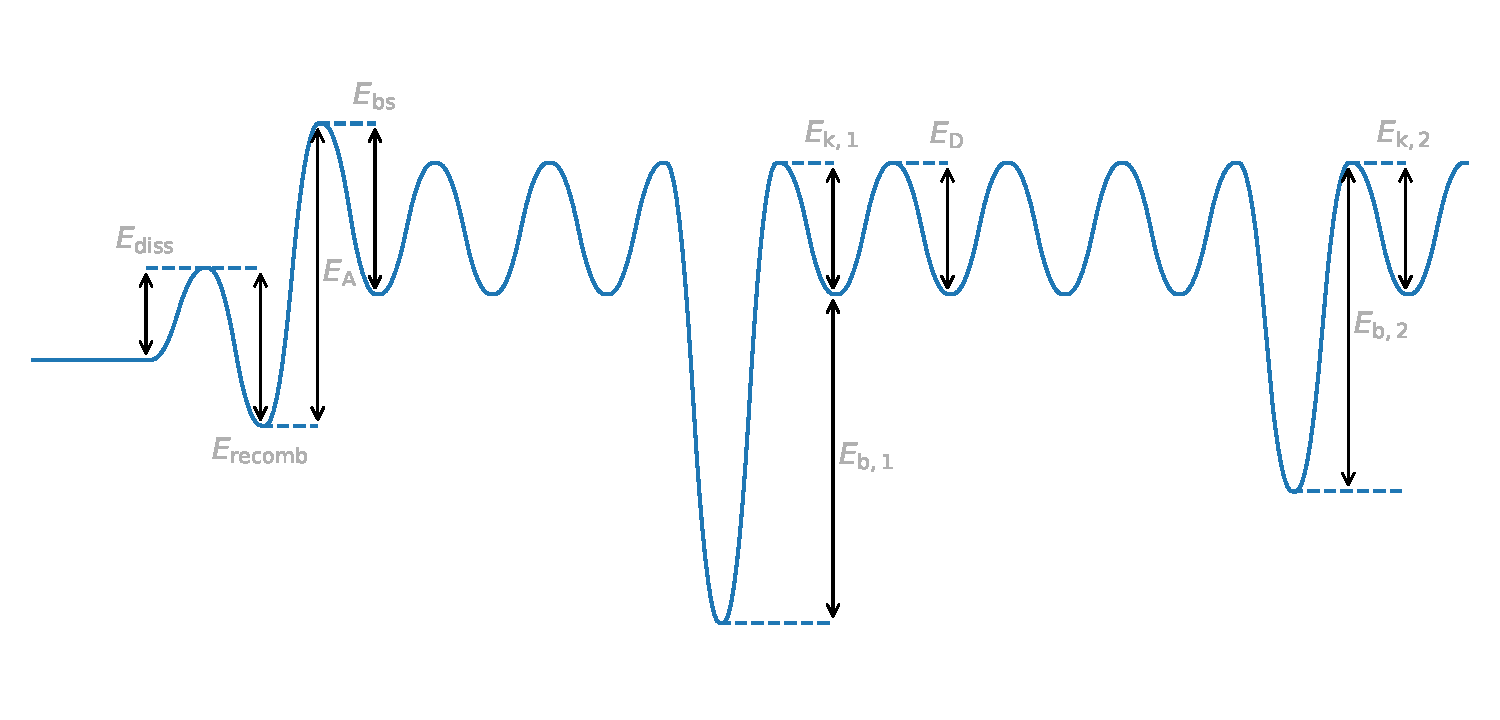
\includegraphics[width=\linewidth]{Figures/Chapter1/potential_energy_diagram.pdf}
    \caption{Simplified potential energy diagram showing two different types of defects.}
    % \end{subfigure}
    % \begin{subfigure}{\linewidth}
    %     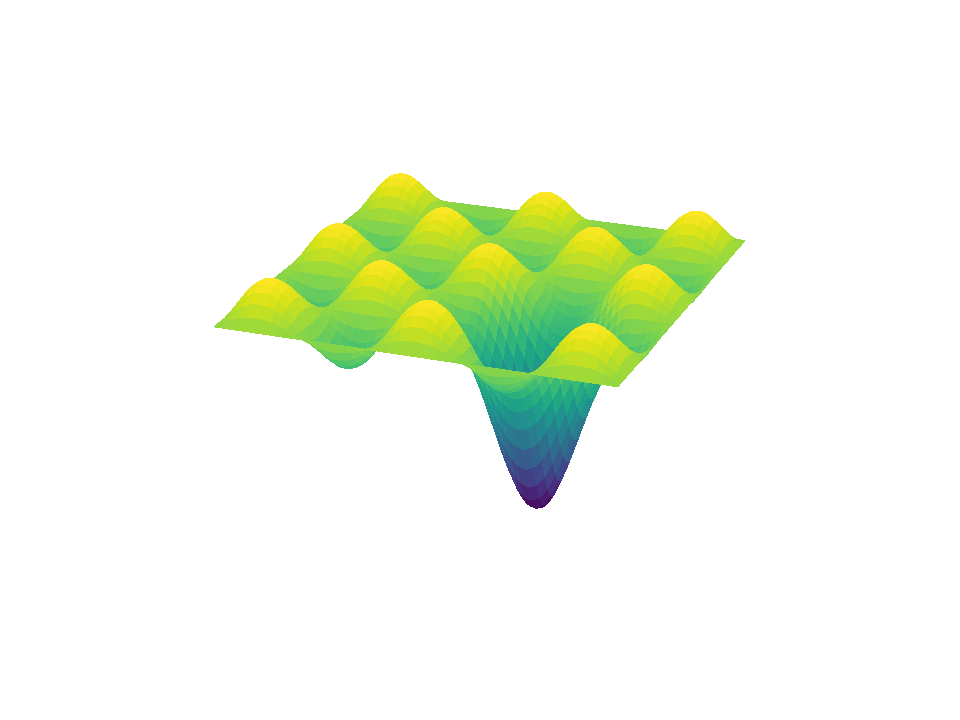
\includegraphics[width=\linewidth]{Figures/Chapter1/potential_energy_3D.pdf}
    %     \caption{3D representation of the potential energy of a solute species in a metal lattice with one defect.}
    % \end{subfigure}
    \labfig{potential energy diagram metal lattice}
\end{figure}

\subsubsection{Diffusion}
The repulsion of metal atoms with solute species creates wells of potential energy located at interstitial sites (see \reffig{potential energy diagram metal lattice}).
The soluted atoms in metals can then jump from interstitial site to another thanks to thermal vibration.
This process is called \emph{\gls{diffusion}}.
The `height` of the potential energy wells is called the \gls{diffusion} \textit{activation energy} or \textit{energy barrier} $E_D$.
\Gls{diffusion} is therefore a thermally activated process governed by a diffusion coefficient $D$ expressed in \si{m^2.s^{-1}}, which follows an Arrhenius law:
\begin{equation}
    D = D_0 \exp{(-E_D/k_B T)}
\end{equation}
where $E_D$ is expressed in \si{eV}, $T$ is the temperature in \si{K}, $k_B$ is the Boltzmann constant in \si{eV.K^{-1}}.

\Gls{diffusion} can also be assisted by temperature gradients (called the \emph{\gls{Soret effect}} or \emph{\gls{thermophoresis}}) \sidecite{martinez_thermal_2021, hodille_estimation_2017, longhurst_soret_1985} or hydrostatic pressure gradients.
The tungsten property to simulate the \gls{Soret effect} (Soret coefficient or heat of transport) is currently missing from litterature (for hydrogen).
Hodille \textit{et al} used the properties of steel as an approximation \cite{hodille_estimation_2017}.
Bennanoune and coworkers performed hydrogen transport studies with hydrostatic pressure gradients showing it could have an impact of around \SI{10}{\%} in steel components \sidecite{benannoune_multidimensional_2020}.
Studies are currently being performed for tungsten.

% MD simulations
Diffusion coefficients (also called diffusivities) can be computed by \gls{md} and \gls{dft}.
The principle of \gls{md} is to calculate the trajectory of atoms in a simulation box (see \reffig{md faney}).
The trajectory of a particle $i$ in a system of $N$ particles can be computed from Newton's second law of motion:

\begin{equation}
    m_i \vec{a_i} = \sum_{j=1 \, j \neq i}^N \vec{F}_{i,j}
\end{equation}
where $m_i$ is the mass of the particle, $\vec{a_i}$ is its acceleration, $\vec{F}_{i,j}$ is the force applied to the particle due to its interaction with particle $j$.
The forces between atoms is only a function of the interatomic potentials.
These potentials can be found in literature or can be estimated from \textit{ab initio} computations (\gls{dft}) \sidecite{boisse_modelling_2014,boisse_modeling_2014} or from methods based on machine learning \sidecite{lam_modeling_2021,behler_constructing_2015}.

\begin{figure*}
    \centering
    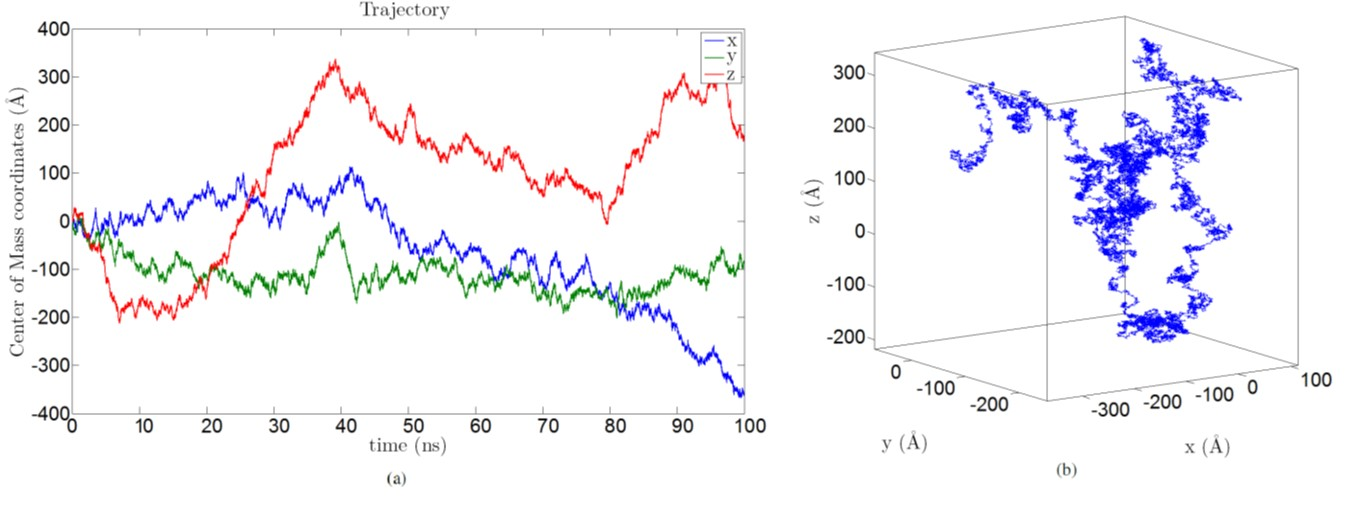
\includegraphics[width=\linewidth]{Figures/Chapter1/faney_md.jpg}
    \caption{Example of the trajectory of a He$_2$ cluster in tungsten. Reproduced from \cite{faney_numerical_2013}.}
    \labfig{md faney}
\end{figure*}

By measuring the trajectory of a diffusing species from \gls{md} simulations for a long time, its diffusion coefficient $D$ can be estimated from Einstein equation \cite{einstein_uber_1905}:
\begin{equation}
    \lim_{t\to\infty} \frac{\langle R^2(t) \rangle}{6t} = D
\end{equation}
where $\langle R^2(t) \rangle$ is the mean squared displacement of the species.

This modelling technique was used to estimate the diffusion coefficient of \gls{H} in \gls{W} \sidecite{wang_molecular_2020, zhou_molecular_2016,kato_super-saturated_2015,liu_hydrogen_2014} and for He in \gls{W} \sidecite{faney_numerical_2013,faney_spatially_2014,faney_spatially_2015,sefta_surface_2013,perez_mobility_2017}.

% Experiments
Diffusivity of hydrogen has also been measured experimentally in \gls{W} \sidecite{holzner_solute_2020, frauenfelder_solution_1969, anderl_hydrogen_1990}, copper and copper alloys (CuCrZr) \sidecite{anderl_deuterium_1992} and other metals.
Note that the diffusion coefficients measured experimentally are usually effective coefficients accounting for \gls{trapping} effects (detailed below).
% EUROFER \sidecite{montupet-leblond_permeation_2021,esteban_hydrogen_2007,aiello_hydrogen_2002}, 
Because He tends to cluster (as explained below), measuring its diffusivity experimentally is extremely complicated and therefore most estimations of He diffusion coefficients are numerical.
\reffig{diffusivity materials} is a collection of diffusivity values found in literature (measured experimentally or computed) for tungsten, copper and CuCrZr.

% The diffusivities of copper and CuCrZr are comparable (see \reffig{diffusivity solubility copper} and \reffig{diffusivity solubility cucrzr}).

\begin{figure}
    \centering
    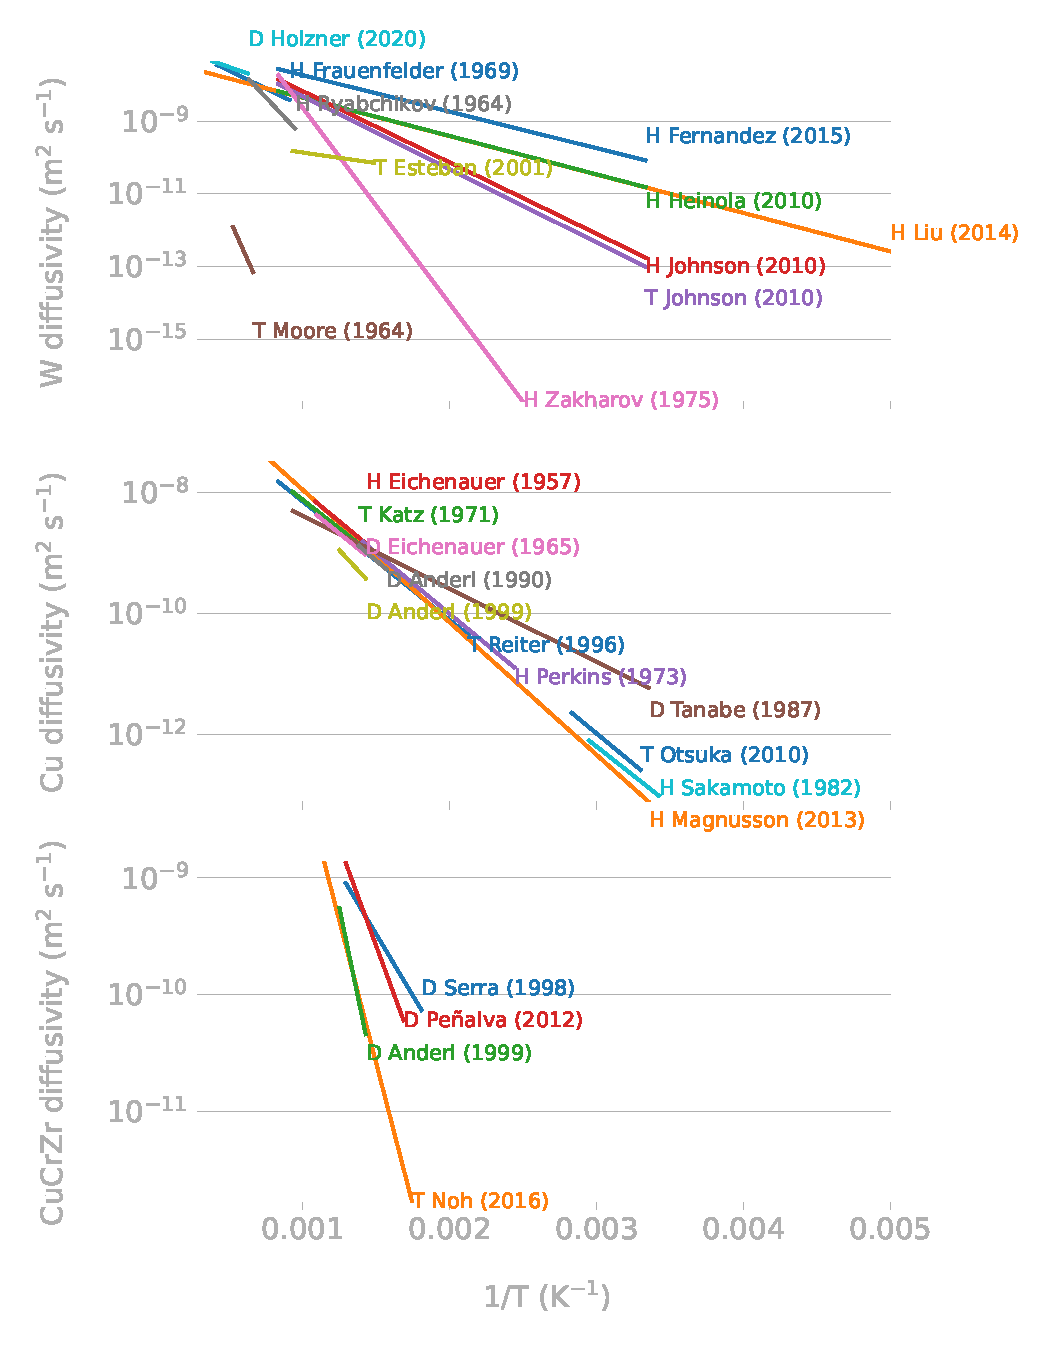
\includegraphics[width=0.75\linewidth]{Figures/Chapter1/materials_diffusivity_review_comparison.pdf}
    \caption{Diffusivity values for tungsten, copper and CuCrZr. Data from \cite{delaporte-mathurin_remdelaportemathurinh-transport-materials_2022}.}
    \labfig{diffusivity materials}
\end{figure}

\subsubsection{Trapping at defects}

Due to the repulsion between solute species and the surrounding metal atoms, defects can act as wells of potential energy for solute species (see \reffig{potential energy diagram metal lattice}).
Once in that attractive well, species can escape it only if their kinetic energy (i.e.\ the temperature) is high enough.
Species can be trapped at \glspl{vacancy}, \glspl{dislocation loop}, \gls{self-interstitial} atoms (in the case of hydrogen in tungsten), impurities, etc.

The \gls{trapping} process can be described as:
\begin{equation}
    \ce{S + T <=>[k][p] S^*}
\end{equation}
where S is the particle in an interstitial site (i.e.\ mobile), T is the defect and S$^*$ represents the particle trapped in the defect T.
The \gls{trapping} rate and \gls{detrapping} rate can be respectively expressed as:
\begin{align}
    k &= k_0 \exp{\frac{-E_k}{k_B T}} \\
    p &= p_0 \exp{\frac{-(E_\mathrm{b} + E_k)}{k_B T}} = p_0 \exp{\frac{-E_p}{k_B T}}
\end{align}
where $E_k$ is the \gls{trapping} energy in \si{eV}, $k_B$ is the Boltzmann constant in \si{eV.K^{-1}}, $T$ is the temperature in \si{K}, $E_\mathrm{b}$ is the binding energy of the particle with the defect and $E_p = E_\mathrm{b} + E_k$ is the \gls{detrapping} energy.
A common assumption is that $E_k = E_D$.

Each rate therefore has two parameters: the pre-activation factor and the activation energy.
These parameters can be identified from fitting \gls{tds} experiments.
\gls{tds} experiments consist in loading a metal sample with the studied species (\textit{eg} \gls{H} or \gls{He}) and heat it at different temperatures with a well controlled temperature ramp (\textit{eg} \SI{1}{K.s^{-1}}, \SI{10}{K.s^{-1}}...) while measuring the desorption flux.
This results in a spectrum which typically has one or several desorption peaks corresponding to different traps (see \reffig{TDS example ialovega}).
Peaks appearing at high temperatures correspond to ``deep'' traps with a high \gls{detrapping} energy $E_p$.

\begin{figure} [h!]
    \centering
    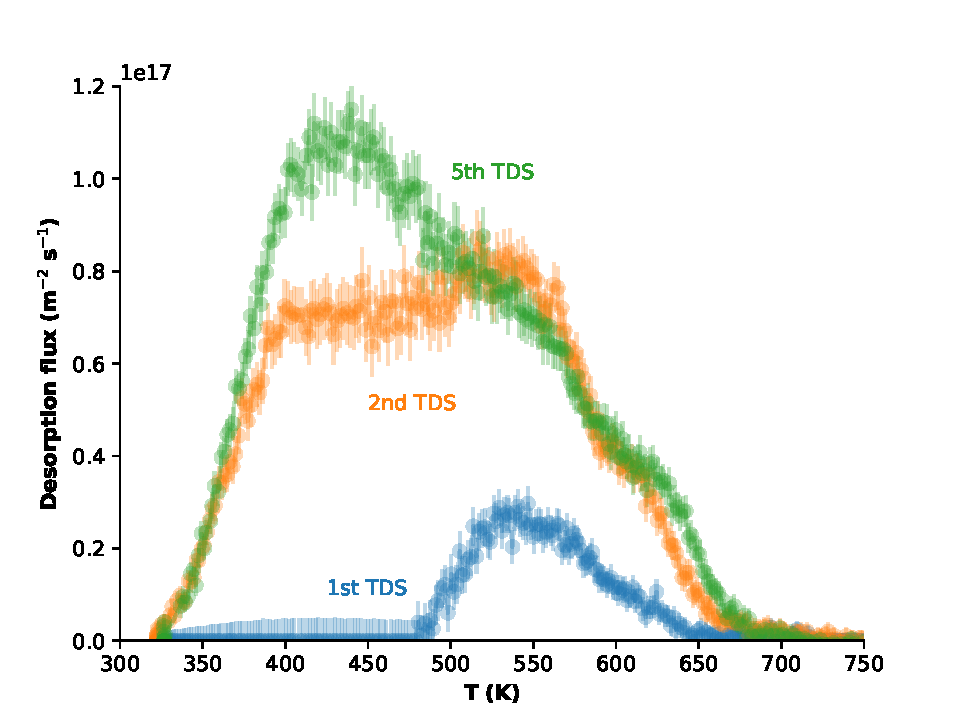
\includegraphics[width=\linewidth]{Figures/Chapter1/tds_helium_nicolas.pdf}
    \caption{H TDS spectra of pre-damaged W. Reproduced from \cite{ialovega_hydrogen_2020}.}
    \labfig{TDS example ialovega}
\end{figure}

These parameters can also be obtained from \gls{dft} calculations \sidecite{hou_predictive_2019, backer_hydrogen_2017, backer_multiscale_2017, fernandez_hydrogen_2015, lu_review_2014, heinola_hydrogen_2010, zhou_investigating_2010}.

Some defects can trap several hydrogen/helium atoms.
For instance, up to approximately seven helium atoms can be trapped in a mono-\gls{vacancy} \sidecite{faney_spatially_2015}.
\gls{dft} calculations also show that defects like mono-vacancies, dislocations or grain boundaries can retain multiple hydrogen atoms (see \reffig{trapping energy hydrogen in tungsten}).
As the number of trapped particles (helium or hydrogen) increases, the binding energy of a particle with the defect usually decreases.
In other words, the more particles are trapped in a defect the easier it is for a hydrogen atom to escape.
For instance, the binding energy of a helium atom in an empty mono-\gls{vacancy} is around \SI{4}{eV} and around \SI{2.5}{eV} if the \gls{vacancy} already retains four helium atoms \cite{faney_spatially_2015}.
Similarly, the binding energy of a hydrogen atom in a mono-\gls{vacancy} varies from \SI{0.5}{eV} (with six hydrogen atoms trapped) to \SI{1.3}{eV} (empty \gls{vacancy}) (see \reffig{trapping energy hydrogen in tungsten}).

\begin{figure*}
    \centering
    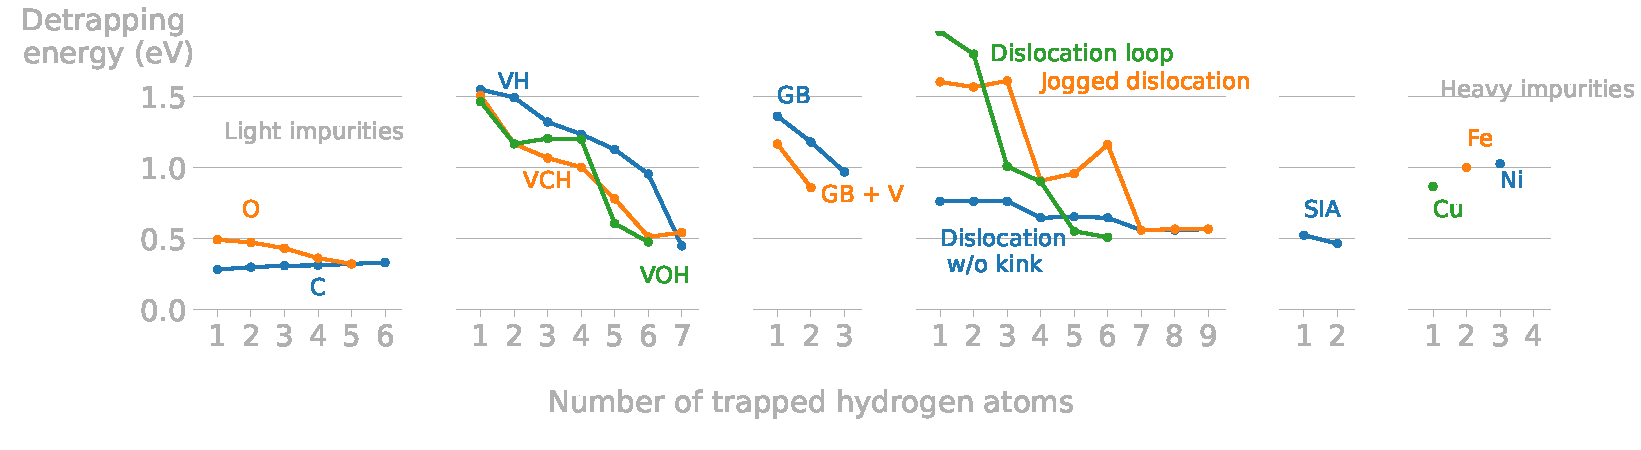
\includegraphics[width=\linewidth]{Figures/Chapter1/trapping_energy_hydrogen_in_tungsten.pdf}
    \caption{Detrapping energy of a hydrogen atom in several defects in tungsten: vacancies, impurities, self-interstitial atoms (SIA), grain boundaries (GB), in tungsten depending on the number of trapped hydrogen atoms. Reproduced from \cite{hodille_study_2016}.}
    \labfig{trapping energy hydrogen in tungsten}
\end{figure*}

Defects can either be pre-existent in the material (sometimes called \textit{intrinsic} defects): impurities, grain boundaries, etc.
They can also be created from external factors (\textit{extrinsic} defects) like particle bombardment (ions, neutrons) \sidecite{ogorodnikova_deuterium_2003} or mechanical stress \sidecite{benannoune_multidimensional_2020}.

\subsubsection{Surface dissolution}

When a surface is in contact with a gas, molecular species (\textit{eg.} $\text{H}_2$, $\text{T}_2$, $\text{HD}$...) can dissociate into mono-atomic species.
After their dissociation, the atomic particles can be adsorbed on the surface (on adsorption sites).
This dissociation is described by a sticking propability usually associated with an Arrhenius law $s = s_0 \exp{(-E_s/k_B T)}$.
\gls{dft} calculations can calculate energy barriers for adsorption and migration of solute species on surfaces \sidecite{heinola_first-principles_2010}.
Studies have however shown that this process is not thermally activated (i.e.\ $E_s=0$) \sidecite{alnot_adsorption_1989, tamm_interaction_1970} but rather depends on the ratio of the surface concentration of the species (hydrogen or helium) by the concentration of adsorption sites.
This quantity is called the \textit{surface coverage} $\theta$. 
When $\theta = 1$, the surface is fully saturated and when $\theta = 0$ all the adsorption sites are available.
Moreover, the presence of impurities occupying adsorption sites can decrease the sticking probability of a species \sidecite{dunand_surface_2022, whitten_coadsorption_1998}.

Adsorbed particles can then be \textit{absorbed} in the bulk (see \reffig{potential energy diagram metal lattice}).
This thermally activated process is associated with an absorption coefficient following an Arrhenius law $A=A_0 \exp{(-E_A/k_B T)}$.
The absorption process is modelled using \gls{dft} and absorption activation energies $E_A$ can be determined for different surface orientations \sidecite{johnson_hydrogen_2010, nojima_theoretical_2007,ajmalghan_surface_2019}.

All these processes (dissociation, adsorption and absorption) can be described by an absorption flux:
\begin{equation}
    \varphi_\mathrm{abs} = n K_\mathrm{abs} P
\end{equation}
where $n$ is the absorption order, $K_\mathrm{abs}$ is the absorption coefficient expressed in \si{m^{-2}.s^{-1}.Pa^{-1}} and $P$ is the partial pressure of hydrogen in \si{Pa}.

Desorption of solute species at the surface is expressed by a desorption flux:
\begin{equation}
    \varphi_\mathrm{des} = K_\mathrm{des} c_\mathrm{surface}^n
\end{equation}
where $K_\mathrm{des}$ is the desorption coefficient expressed in \si{m^{-2+3n}.s^{-1}}, $c_\mathrm{surface}$ is the surface concentration in \si{m^{-3}}, and $n$ is the order of the desorption.

When the equilibrium between absorption and desorption is reached, $\varphi_\mathrm{abs} = \varphi_\mathrm{des}$, which gives:
\begin{equation}
    n K_\mathrm{abs} P = K_\mathrm{des} c_\mathrm{surface}^n
    \labeq{equilibrium absorption desorption}
\end{equation}

By rearranging \refeq{equilibrium absorption desorption}:
\begin{equation}
    c_\mathrm{surface} = \sqrt[n]{n \frac{K_\mathrm{abs}}{K_\mathrm{des}}} \sqrt[n]{P}
\end{equation}

When the absorption/desorption order is $n=1$ (monoatomic absorption):
\begin{equation}
    c_\mathrm{surface} = K_H P
\end{equation}
This relationship is known as Henry's law of solubility and $K_H = K_\mathrm{abs}/K_\mathrm{des}$ is the material solubility expressed in \si{m^{-3}.Pa^{-1}}.

When the absorption/desorption order is $n=2$ (diatomic absorption):
\begin{equation}
    c_\mathrm{surface} = K_S \sqrt{P}
    \labeq{sievert's law}
\end{equation}
This equilbrium is known as Sievert's law of solubility and $K_S = \sqrt{2 K_\mathrm{abs}/K_\mathrm{des}}$ is the material solubility expressed in \si{m^{-3}.Pa^{-0.5}}.
The solubility of tungsten, copper and CuCrZr are described in \reffig{solubility materials}.

The product of the solubility and diffusivity is called \textit{permeability}.

\begin{figure}
    \centering
    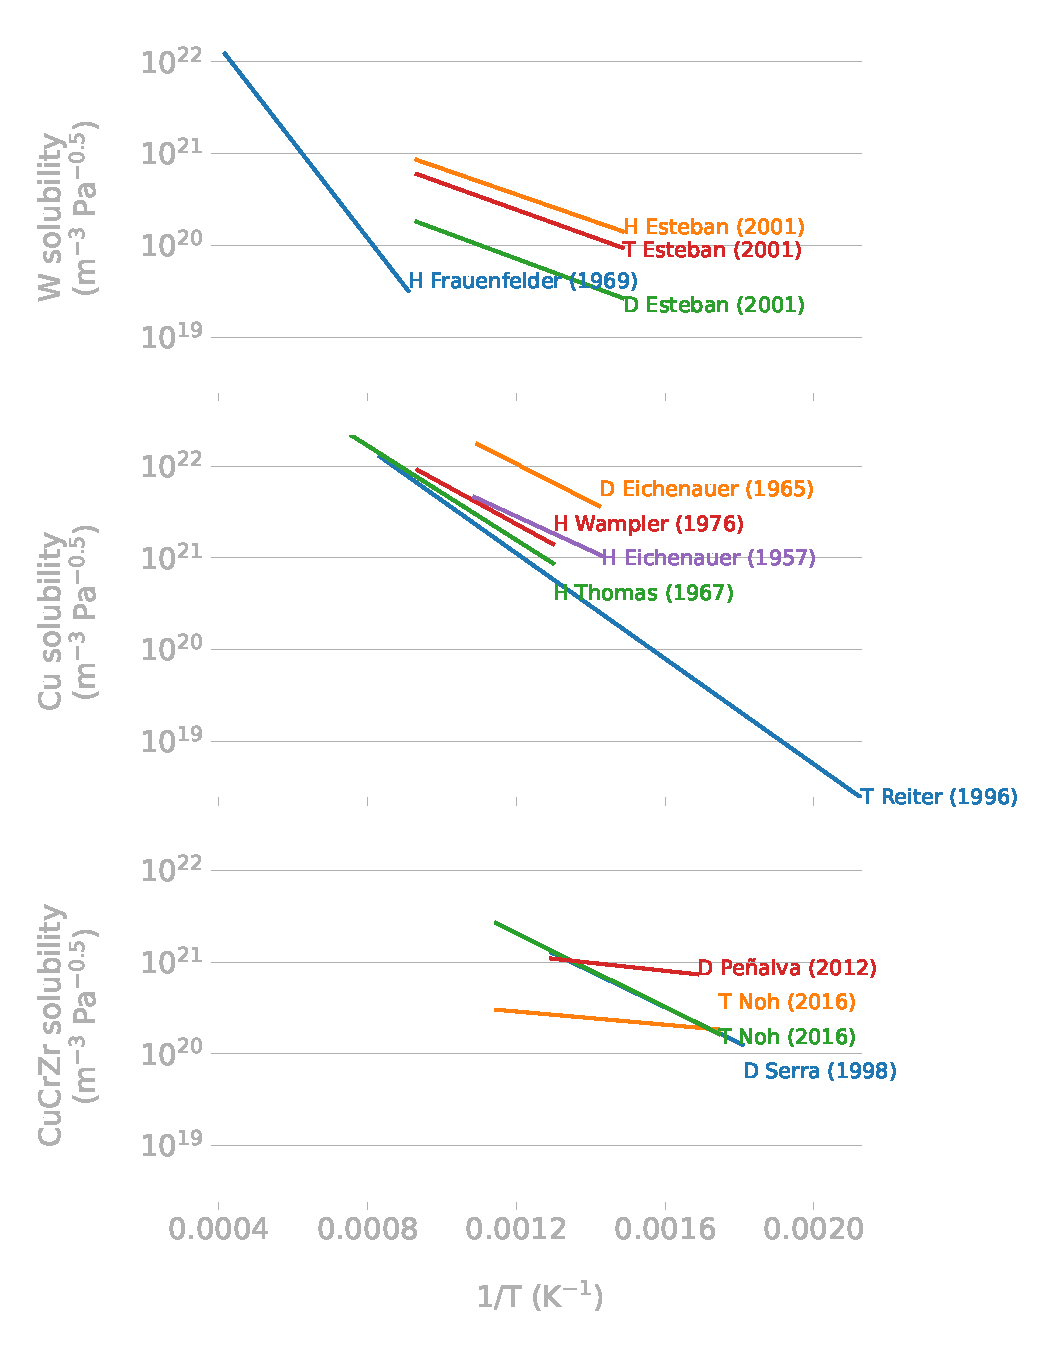
\includegraphics[width=0.75\linewidth]{Figures/Chapter1/materials_solubility_review_comparison.pdf}
    \caption{Solubitity values for tungsten, copper and CuCrZr. Data from \cite{delaporte-mathurin_remdelaportemathurinh-transport-materials_2022}.}
    \labfig{solubility materials}
\end{figure}

\subsubsection{Interface between materials}
At the interface between two materials, the continuity of chemical potential has to be ensured \sidecite{krom_hydrogen_2000}.
The continuity of chemical potential is conveyed by the continuity of $P$, the local partial pressure of hydrogen at equilibrium.
In a metal, $P$ can be expressed from Sievert's law of solubility (see \refeq{sievert's law}):
\begin{equation}
    P = (c_\mathrm{m}^-/S^-)^2
\end{equation}
with $c_\mathrm{m}$ the concentration of mobile species in the material, $S$ the solubility in the materials expressed in \si{m^{-3}.Pa^{-0.5}}.
% A way to picture the continuity of chemical potential is to imagine a gas layer at the interface between two materials at a partial pressure $P_\mathrm{eq}$.
% $P_\mathrm{eq}$ can be expressed by the solubility law at the surface of each material.
At the interface between two metallic surfaces, the chemical potential continuity is therefore conveyed by the continuity of the quantity $c_\mathrm{m}/S$:
\begin{equation}
    (c_\mathrm{m}^-/S^-)^2 = (c_\mathrm{m}^+/S^+)^2
    \labeq{c/s conservation}
\end{equation}

In the case of a metal in contact with a non-metallic liquid behaving according to Henry's law (\textit{eg} a molten salt):
\begin{equation}
    (c_\mathrm{m}^-/S^-)^2 = c_\mathrm{m}^+/S^+
\end{equation}
with $S$ the solubility of \gls{H} in the materials expressed in \si{m^{-3}.Pa^{-0.5}} or \si{m^{-3}.Pa^{-1}}.

A jump in concentration will therefore occur at the interface bewteen two materials with different solubilities.

\subsubsection{Advection in liquids}
\Gls{advection} occurs when a mobile species is in a liquid (molten salts, water, coolants...) and depends on the liquid velocity.
This advective transport adds up to the diffusive transport.

Depending on the liquid velocity and the species diffusivity in this liquid, the mass transport can be predominated by one of the two phenomena.
The Péclet number $\mathrm{Pe}$ is a dimensionless number employed to estimate this dominance.

\begin{equation}
    \mathrm{Pe} = \frac{\mathrm{advective \; transport \; rate}}{\mathrm{diffusive \; transport \; rate}} = \frac{L u}{D}
\end{equation}
where $L$ is a charasteristic length, $u$ is the fluid velocity and $D$ is the species diffusivity in this fluid.

When $\mathrm{Pe} \gg 1$, \gls{advection} is the dominant transport phenomena.
When $\mathrm{Pe} \ll 1$, \gls{diffusion} dominates and \gls{advection} can be neglected.

For hydrogen diffusing in liquid LiPb (typically in a WCLL breeding blanket with a charasteristic length $L \approx \SI{1}{m}$), with $D \approx \SI{1e-9}{m^2.s^{-1}}$ and $u \approx \SI{1e-4}{m.s^{-1}}$ \sidecite{dark_influence_2021}, $\mathrm{Pe} \approx 10^{5}$, which means that \gls{advection} dominates the mass transport and cannot be neglected.

\subsubsection{Clustering}
Single He atoms implanted into the material diffuse rapidly due to the high W-He repulsion.
This high repulsive W-He interaction is such that interstitial He atoms preferably rearrange into groups of atoms in order to minimise the number of repulsive interactions \sidecite{hamid_molecular_2019, hammond_large-scale_2018}.
This phenomena, called \emph{clustering}, was highlighted by \gls{dft} studies \cite{becquart_density_2009,dunn_rate_2013} and MD simulations \cite{henriksson_molecular_2006}.
Small clusters are themselves mobile as long as all the He atoms within the cluster are occupying interstitial position in the solid \gls{lattice}.
The activation energy for interstitial He atoms and clusters in \gls{W} ranges from 0.15 to \SI{0.45}{eV} according to Perez \textit{et al} \sidecite{perez_mobility_2017}.
He clusters will eventually grow by interacting with either interstitial He atoms or other clusters.

Clustering of \gls{H} atoms is less clear and Henriksson \textit{et al} showed that \gls{H} atoms do not form bonds with other \gls{H} atoms in \gls{bcc} \gls{W} \sidecite{henriksson_difference_2005}.

\subsubsection{Bubble nucleation}

If its size is big enough the cluster pressure is sufficient to knock off a \gls{W} atom from the \gls{lattice}, creating a \gls{W} \gls{vacancy} and an interstitial \gls{W} atom (a \gls{Frenkel pair}).
This process is called \gls{trap mutation} or \emph{\gls{self-trapping}} and the trapped clusters act as nuclei for bubble formation.

\Gls{trap mutation} has been modelled in \gls{W} using \gls{dft} \sidecite{boisse_modelling_2014} and Monte Carlo computations \sidecite{de_backer_modeling_2015}.
It has been shown that this phenomena depends not only on the number of He atoms in the cluster but also on temperature, position of the cluster to the free surface or even the crystal orientation \sidecite{blondel_modeling_2017, hu_interactions_2014, hu_dynamics_2014}.
At this point, the trapped cluster occupies the newly created \gls{W} \gls{vacancy} position.
It is considered immobile since it would require either diffusion of another \gls{vacancy} next to it, or recombination of the Frenkel pair in order to diffuse \sidecite{morishita_nucleation_2007}.

\subsubsection{Bubble growth}

\begin{figure} [h!]
    \centering
    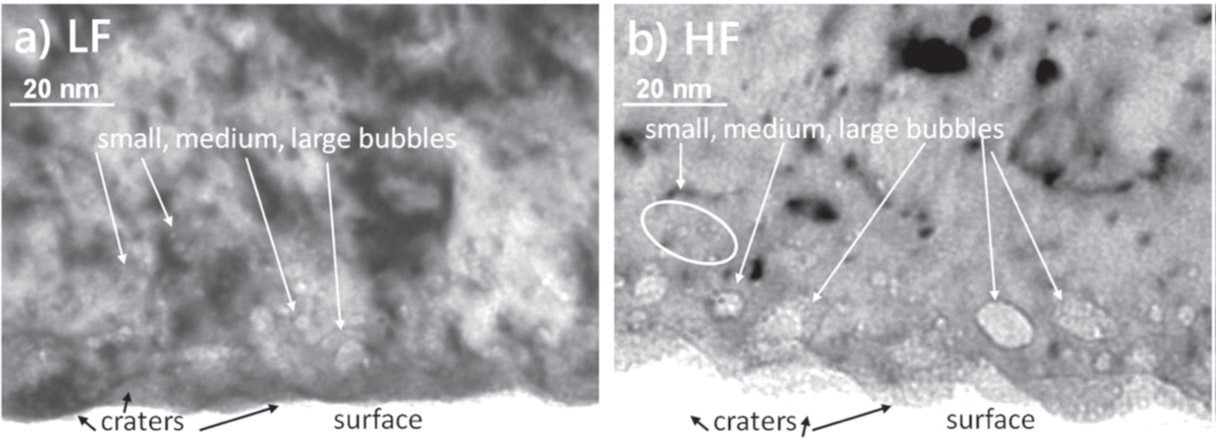
\includegraphics[width=\linewidth]{Figures/Chapter1/helium_bubbles_ialovega.jpg}
    \caption{Transmission electron microscopy image of tungsten irradiated with He ions at different fluxes (Low Flux (LF) = \SI{2.9e20}{m^{-2}.s^{-1}} and High Flux (HF) = \SI{2.3e22}{m^{-2}.s^{-1}}) showing the presence of He bubbles. Reproduced from \cite{ialovega_hydrogen_2020}.}
    \labfig{he bubbles ialovega}
\end{figure}

Once a bubble nucleus is created via \gls{trap mutation}, it can continue to grow via three main mechanisms: absorption of clusters, \gls{loop punching} or blistering.
Two or more bubbles can also coalesce and form a bigger bubble.
Condon and Schober \sidecite{condon_hydrogen_1993} reviewed the key mechanisms of bubble growth in metals.

Each of these mechanisms can become dominant over another depending on the implantation and the metal conditions. 
Bubbles can continue to grow by absorbing interstitial He atoms or mobile He clusters (i.e.\ that haven't self trapped).
Considering that vacancies are mobile in the solid, the volume of a bubble could also increase if a \gls{vacancy} or a \gls{vacancy} cluster interacts with a He bubble.
The same is true for He-vacancies or H-vacancies clusters.

There is no experimental evidence of He clustering with \gls{self-interstitial} \gls{W} atoms \sidecite{faney_spatially_2014}.

% This process is described by cluster dynamics equations in which interaction between the clusters is governed by pairs of association and dissociation rates.
During the growth of a He bubble by absorbing He atoms, if the pressure increases until reaching a critical value, \gls{dislocation loop} punching can occur.
During the punching event, a whole facet of \gls{W} atoms is pushed and the vacant \gls{lattice} sites are absorbed by the bubble allowing the bubble to expand and reducing the pressure in it \sidecite{sefta_surface_2013}.
The produced \gls{self-interstitial} \gls{W} atoms will likely be attracted by \textit{image forces} at the surface and will contribute to the roughening of the surface and/or formation of surface structures.

\Glspl{dislocation loop} happen at very high pressure and if the number of vacancies in the \gls{lattice} is low compared to the amount of He atoms.
This is the case when a high He flux is applied and the He ions energy is low so that no displacement damaged is produced \cite{sefta_surface_2013}.
If vacancies were created via He ions implantation, they could interact with existing He bubbles which would have the effect of increasing the volume and thus decreasing the pressure (assuming no change in temperature and no other implantation mechanism).

Coalescence of He bubbles has been observed in \gls{md} simulations \sidecite{hamid_molecular_2019, hammond_helium_2019, zhang_simulation_2019} and would tend to increase the bubble size decreasing the bubble density at the same time.
This may not have an impact on He concentration on the macroscopic scale but might influence bubble bursting.

The pressure inside the bubble and the bubble radius are two parameters of interest and are correlated.
Sefta \sidecite{sefta_surface_2013} proposed to use the Wolfer equation of state in order to determine the number of He atoms contained in a He bubble based on its pressure, the latter being calculated from its radius and its surface tension.
One must be aware that if radii and pressure of bubbles computation is quite straightforward using \gls{md} \sidecite{zhang_simulation_2019} or cluster dynamics \sidecite{faney_spatially_2015} simulations it will be more complex to estimate these metrics considering a continuum model that does not keep track of every type of clusters but only a few of them.
The only information \textit{a priori} available in this case is indeed the local helium concentration and an equivalence could be found by either having a high density of small bubbles or a low density of big bubbles.
An effort has been made by Ialovega to measure the pressure inside helium bubbles using \gls{eels} \sidecite{ialovega_surface_2021}.
This technique, consisting in analysing the electron energy loss as they interact with matter \sidecite{pyper_excited_2017}, showed evidence that the observed cavities (see \reffig{he bubbles ialovega}) were filled with helium.

\subsubsection{Blistering}

\begin{figure}
    \centering
    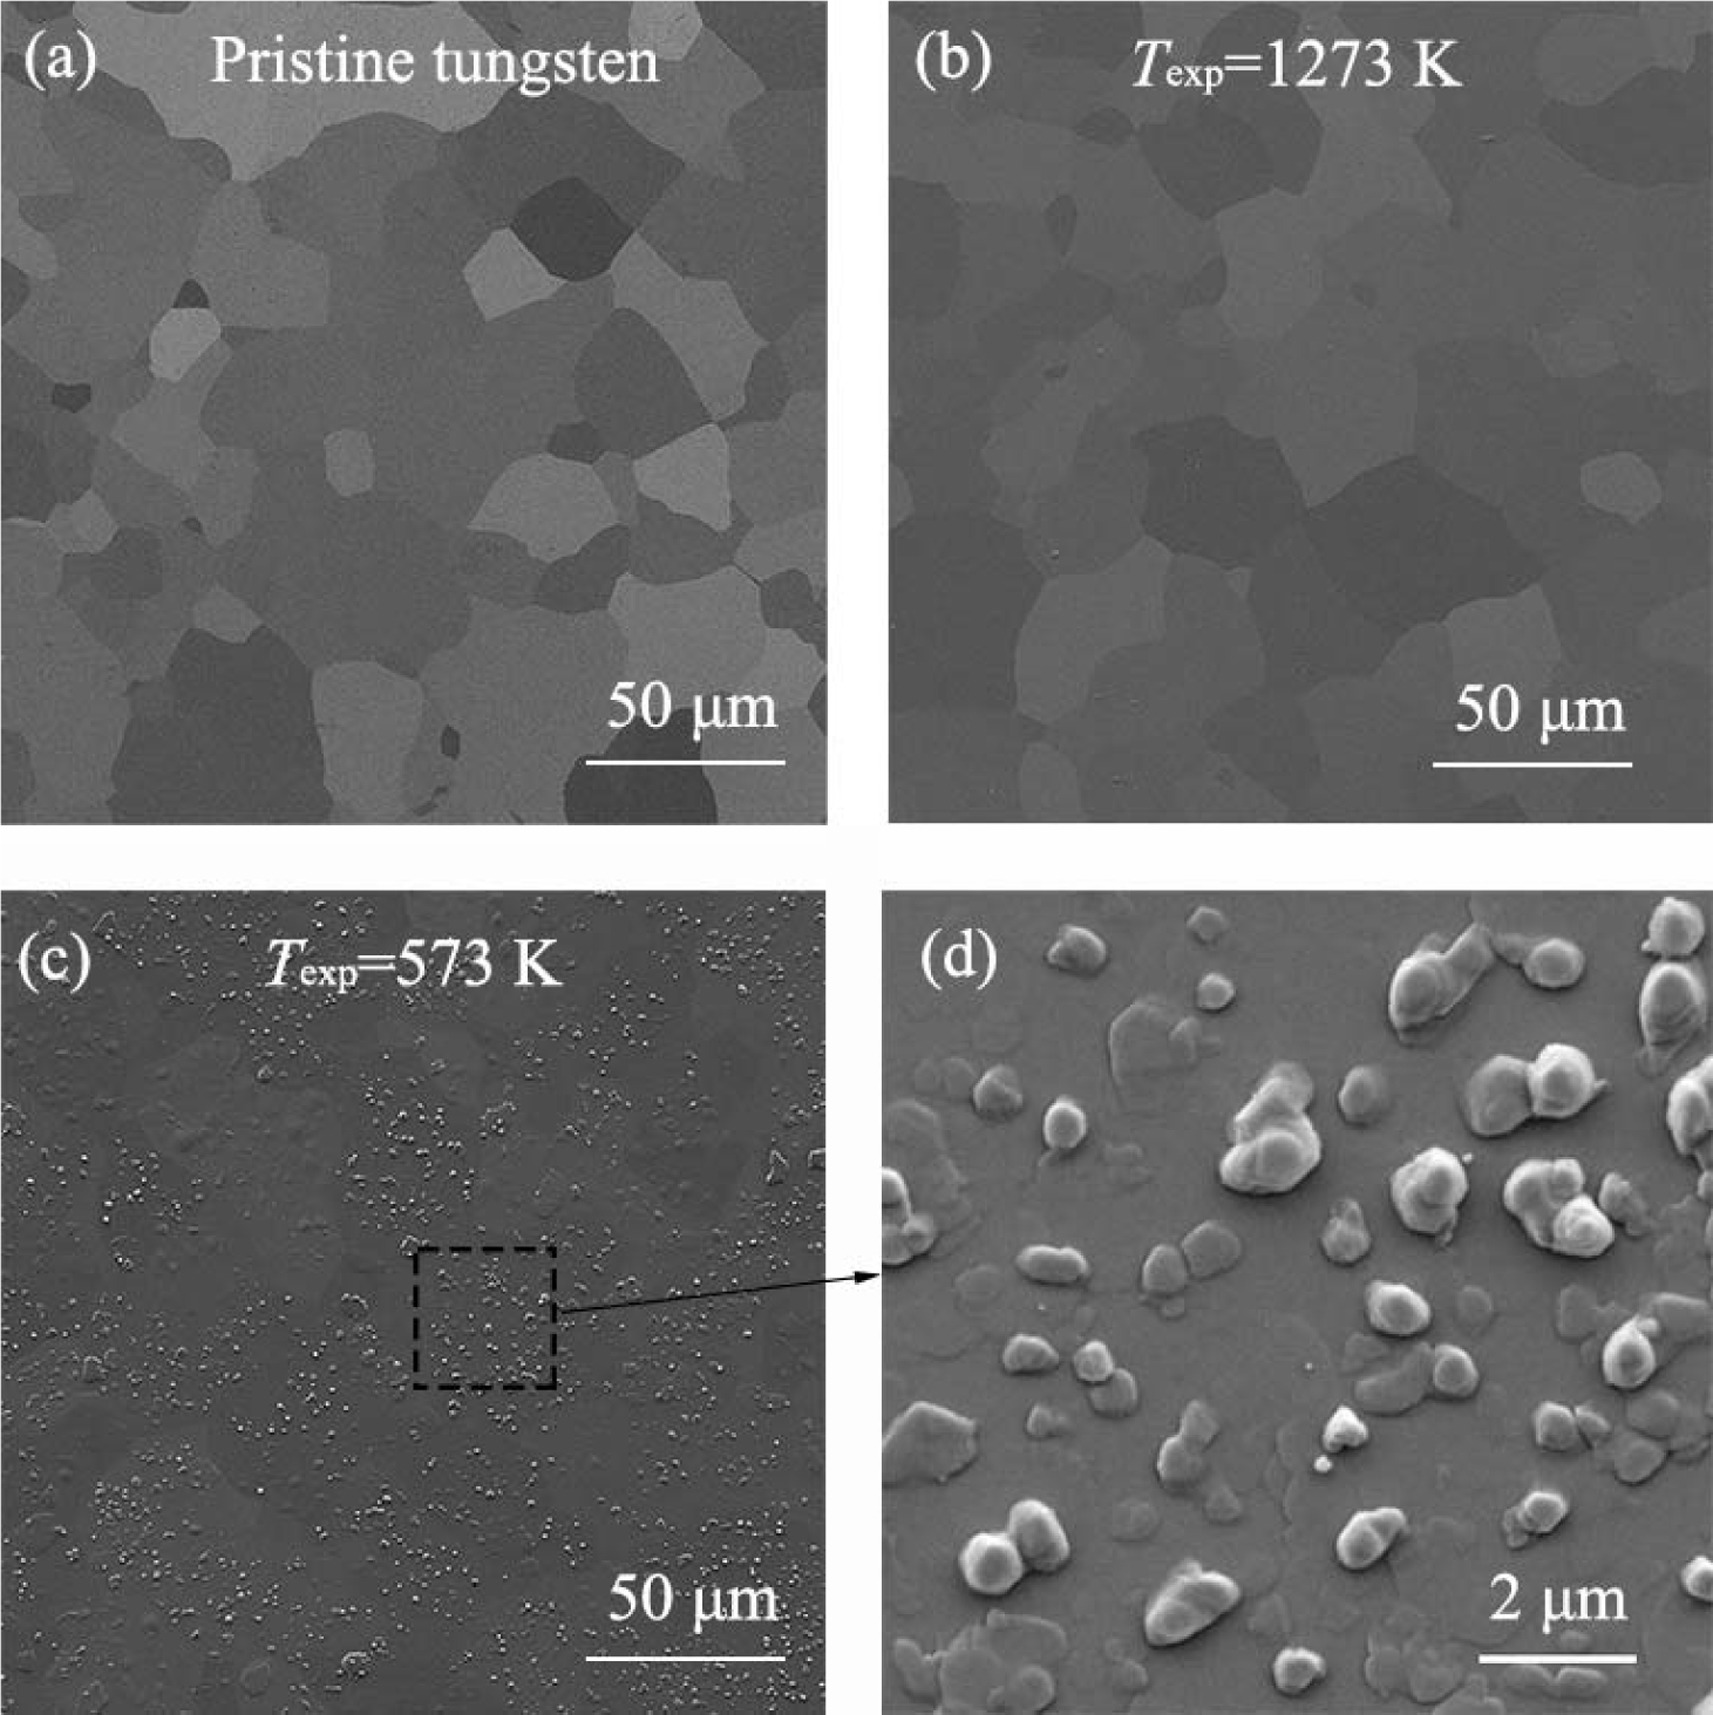
\includegraphics[width=\linewidth]{Figures/Chapter1/h_blisters_in_tungsten.jpg}
    \caption{Scanning Electron Microscopy images of the surface of W samples exposed to \SI{50}{eV} H plasma at \SI{573}{K} and \SI{1273}{K}. Reproduced from \cite{chen_irradiation_2019}.}
    \labfig{h blisters in tungsten}
\end{figure}

During helium or hydrogen implantation, \emph{\gls{blistering}} can be observed under certain conditions.
Blisters are plastic deformation (swelling) of the metal near the surface due to high pressure in bubbles (see \reffig{h blisters in tungsten}).
This phenomenon is separated from \gls{loop punching} even though \gls{loop punching} can be considered as a plastic deformation.
\Gls{blistering} usually happens at low temperatures because only then the growth rate of the bubble is greater than the dissolution in the bulk (which depends on the thermally activated diffusion coefficient and solubility).
Eventually, if the rate of incoming atoms is greater that the rate of re-dissolution in the bulk, blisters can rupture.
Similarly, if the rate of incoming atoms is less than the rate of re-dissolution in the bulk, the blister will collapse.

Helium \gls{blistering} has been observed in \gls{W} at low temperature ($< \SI{1000}{K}$) \sidecite{baldwin_formation_2010}.
Hydrogen \gls{blistering} was also observed in \gls{W} \sidecite{haasz_effect_1999}.
Causey \textit{et al} also reviewed a wide range of studies showing H exposure leads to \gls{blistering} \sidecite{causey_hydrogen_2002}.
\Gls{blistering} was found to lead to hardening in W due to the production of dislocations \sidecite{chen_irradiation_2019}.
It can also form cracks depending on the alloying elements in W and the microstructure \sidecite{ueda_hydrogen_2005}.

Hydrogen \gls{blistering} was observed under high energy irradiation (typically from a few \si{keV} to \si{MeV}).
These energies are orders of magnitudes higher than the ones expected in the \acrshort{iter} \gls{divertor} (see \reffig{divertor exposure conditions}).

It was also found that hydrogen blister formation was avoided in tungsten at temperatures above \SI{600}{K} \sidecite{wang_blister_2001,shimada_blister_2003}.

\subsubsection{Bursting}
% bursting

\begin{figure} [h!]
    \centering
    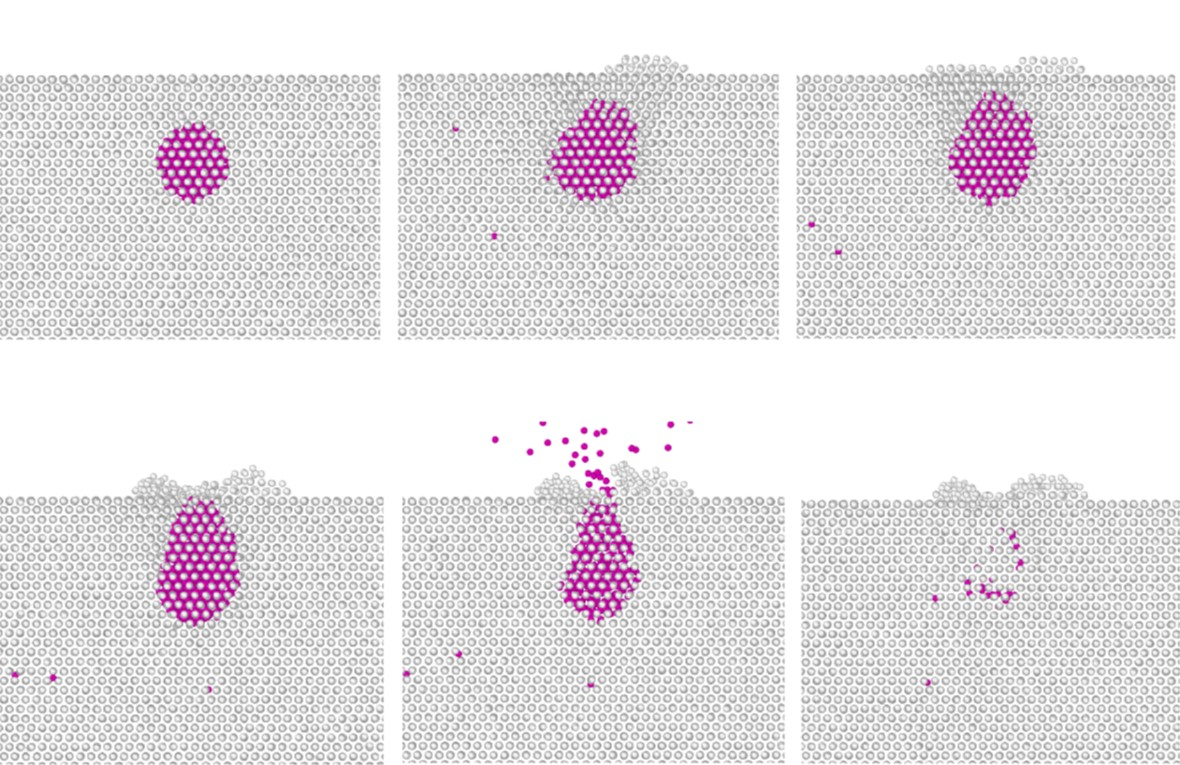
\includegraphics[width=\linewidth]{Figures/Chapter1/bubble_bursting_zhou.jpg}
    \caption{Molecular dynamics simulation of He bubble bursting in W. Reproduced from \cite{zhou_growth_2019}.}
    \labfig{bubble bursting zhou}
\end{figure}

When a bubble grows near the surface and is over-pressurised, \gls{bursting} can occur (see \reffig{bubble bursting zhou}).
As the bubble size increases via \gls{loop punching}, the W \gls{lattice} is deformed and the ligament thickness decreases.
The latter can rupture which would make all the He atoms contained in the bubble to be released to the vacuum.
This is why He \gls{bursting} is characterised by sharp drops in the He \gls{inventory} \sidecite{hammond_helium_2019}.

Sefta and co-workers observed that \gls{bursting} is more likely to happen at high temperatures.
This phenomena contributes to surface roughening and could be the beginning of the formation of \gls{fuzz} \sidecite{sefta_helium_2013}.
Indeed, a \gls{bursting} event could either form a crater on the W surface or an empty cavity due to self-healing.
In the last case, called a \textit{pinhole} \gls{bursting} event, the cavity can be re-pressurised with He atoms.
Blondel \textit{et al} proposed to model \gls{bursting} as a stochastic function of depth in the material rather than a calculation of the bubble pressure.
They have also shown that simulation parameters have an impact on the \gls{retention} \sidecite{blondel_continuum-scale_2018}.
% These differences are mainly due to 2D effects as more bursting events occur but with smaller bubbles.
They have shown that the size of the reaction network size (using cluster dynamics) does not seem to have an influence (between 250 and 200) as the first bursting events happen with clusters of size $\text{He}_{80}$.
% Other simulation parameters (depth of the sample, pre-existing vacancies, bubble growth trajectory...) don't affect the simulations results as they converge for long time steps (100 s).

If \gls{bursting} is not included in continuum simulations, the volume fraction of He present in W could become very large and the dilute limit approximation could no longer be valid \sidecite{sefta_surface_2013}.
The correct metric for estimating \gls{bursting} probabilities must therefore be chosen with care.

\subsubsection{W tendrils or "nano-fuzz"}

\begin{figure} [h!]
    \centering
    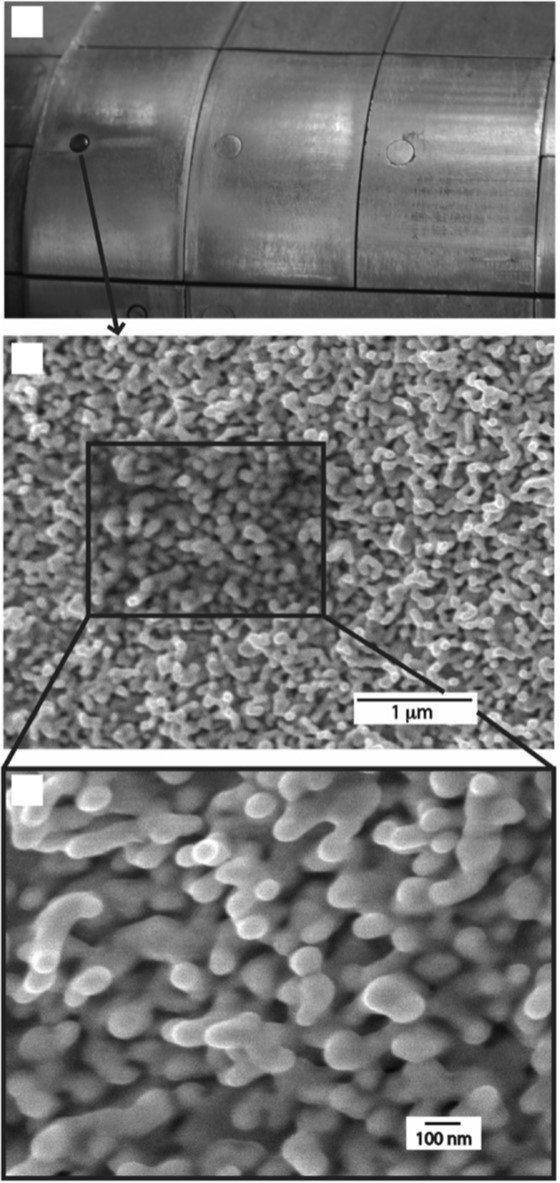
\includegraphics[width=0.5\linewidth]{Figures/Chapter1/fuzz_alcator_wright.jpg}
    \caption{W fuzz observed in Alcator C-Mod. Reproduced from \cite{wright_tungsten_2012}.}
    \labfig{w fuzz wright}
\end{figure}

In 2012, Wright \textit{et al} \sidecite{wright_tungsten_2012} observed the formation of nanostructures on the surfaces of the W divertor of the reactor Alcator C-mod.
These nanostructures are made of W \glspl{tendril} (see \reffig{w fuzz wright}).
These structures are called W \gls{fuzz}, nano-fuzz or even fuzzy W.
Because a small portion of the \gls{divertor} grew W \gls{fuzz}, no conclusion was made regarding its influence on the \gls{plasma} operation.
However, if these structures were to be removed during \gls{plasma} operation via erosion, W atoms could be fed into the \gls{plasma}, affecting the \gls{tokamak} performances.
Moreover, this phenomena could increase the W dust formation in the reactor and lead to contamination and safety issues \sidecite{grisolia_tritium_2015}.

W \gls{fuzz} has been observed at high temperature (>1000K), high flux (>\SI{1e21}{He^+.m^{-2}.s^{-1}}) and long exposure (t>\SI{1e2}{s}) \sidecite{baldwin_formation_2010, nishijima_sputtering_2011}.

The reason of the \gls{fuzz} formation is still unclear but could be due to bursting events and/or accumulation of self interstitial W atoms at the surface \sidecite{baldwin_effects_2009, baldwin_helium_2008, woller_dynamic_2015, hammond_helium_2017}.
Thermal properties of the media are also affected by the formation of W \gls{fuzz} \sidecite{wirtz_influence_2016} which could have a severe impact during ELM-like events.
After 1h of \gls{plasma} implantation, nanostructuring can be found deep in the bulk (up to several hundred of $\mu$m).
According to Baldwin and Doerner \sidecite{baldwin_formation_2010}, heavy alloying helps reducing the formation of He-induced \gls{fuzz}.

Takamura \textit{et al} showed \gls{fuzz} could be grown under relevant \gls{tokamak} conditions (high-flux He \gls{plasma} irradiation and surface temperature greater than \SI{1250}{K}) \sidecite{takamura_formation_2006}.
Baldwin \textit{et al} showed the \gls{fuzz} thickness evolved as a square root of the \gls{fluence} \cite{baldwin_effects_2009}.

\begin{figure} [h!]
    \centering
    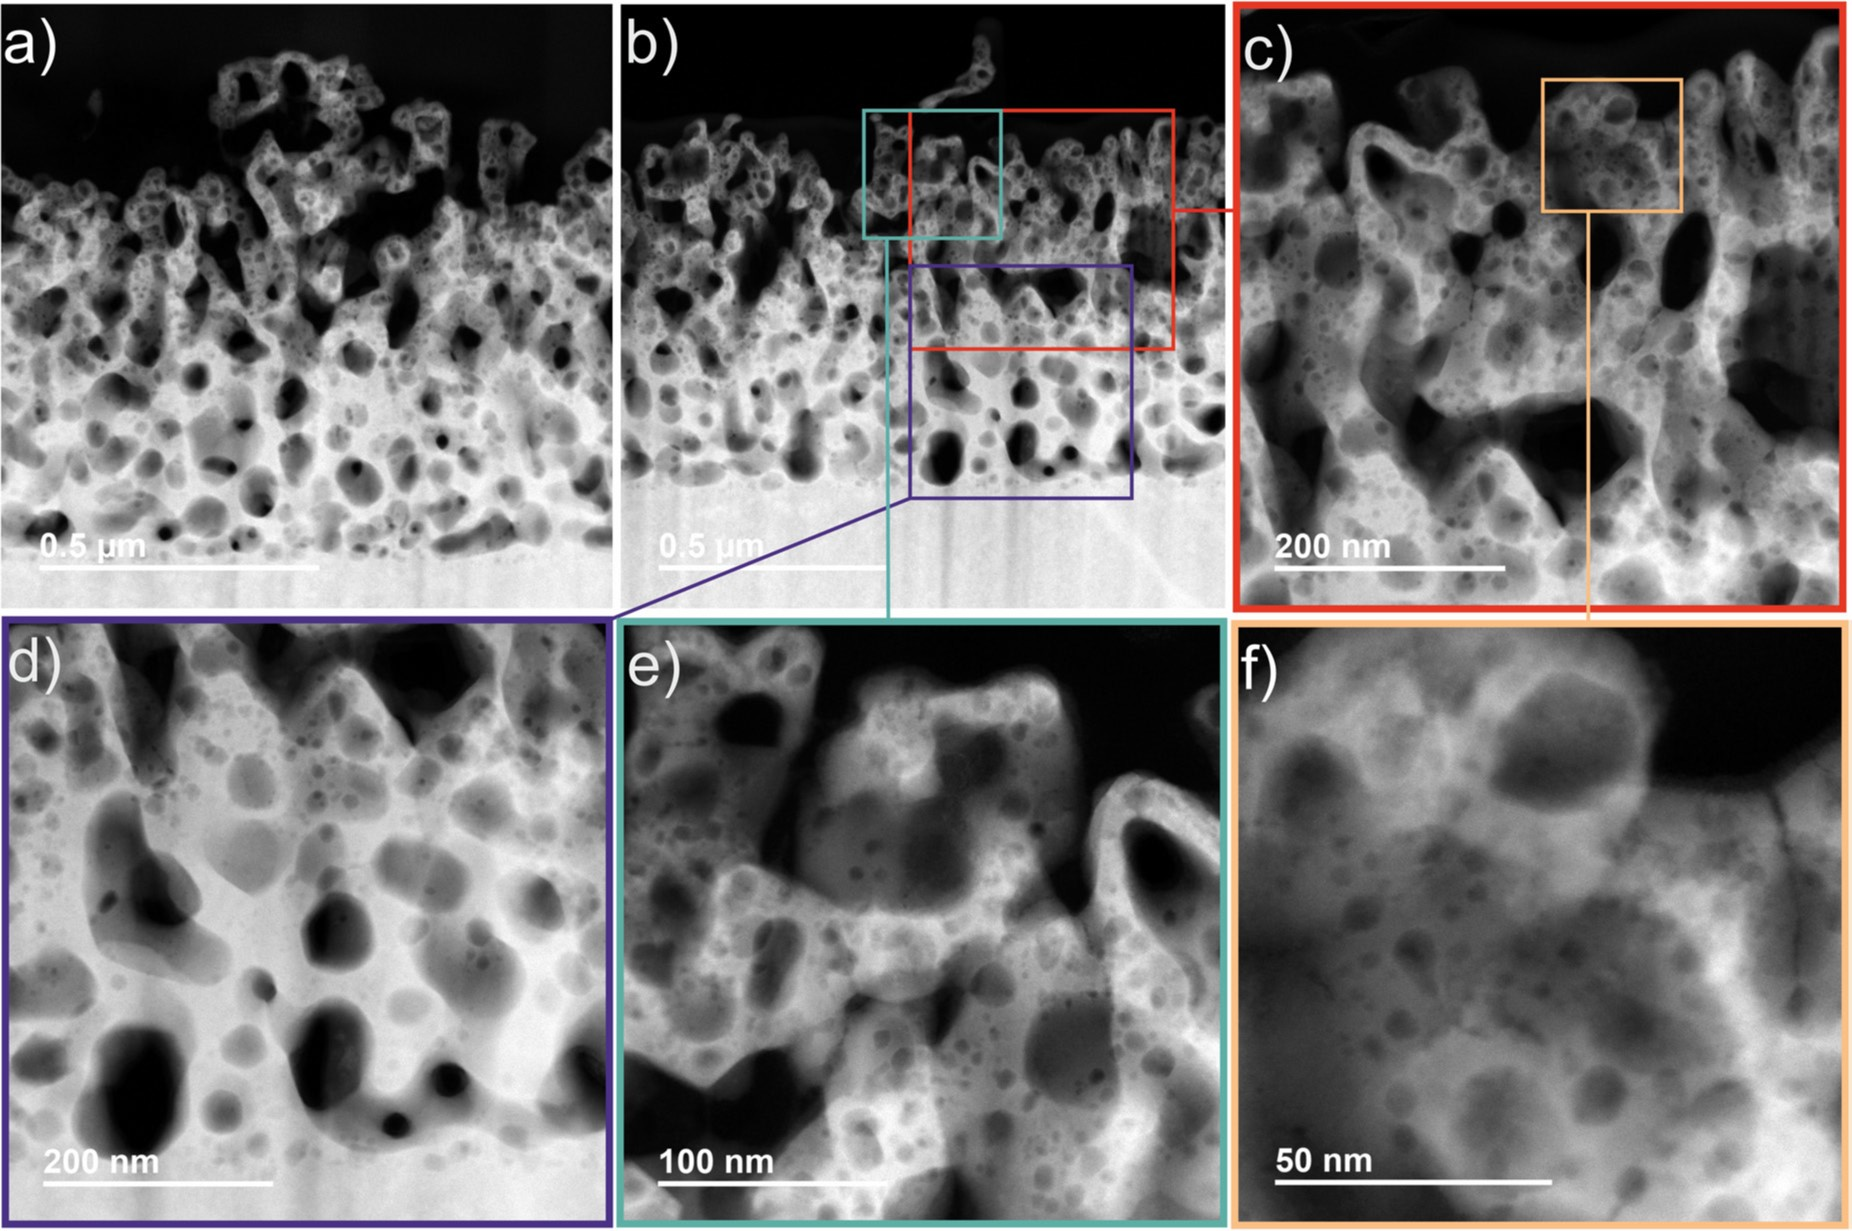
\includegraphics[width=\linewidth]{Figures/Chapter1/fuzz_mccarthy.jpg}
    \caption{Fuzzy W scanning/transmission electron microscopy images showing the presence of He bubbles in tendrils. Reproduced from \cite{mccarthy_enhanced_2020}.}
    \labfig{w fuzz mccarthy}
\end{figure}

McCarthy \textit{et al} studied the formation of W \gls{fuzz} (see \reffig{w fuzz mccarthy}) at helium fluences ranging from \SI{4e23}{m^{-2}} to \SI{e25}{m^{-2}}, temperatures ranging from \SI{1050}{K} to \SI{1150}{K} and He ion energies from \SI{80}{eV} to \SI{100}{eV}.
They identified different \gls{fuzz} growth regimes depending on the He \gls{fluence} due to the change in porosity of the fuzzy layer during the growth process.
The rate of growth was found to be dependent on the temperature and the state (ion or atom) of the incident He particles.

Recent modelling work also showed temperature could significantly affect the bursting of He bubbles and therefore the growth of W \gls{fuzz} \sidecite{niu_effect_2021}.

De Temmerman \textit{et al} concluded that temperature was the most critical parameter controlling W \gls{fuzz} growth \sidecite{de_temmerman_nanostructuring_2012}.

\subsubsection{Cracks}

The role of He implantation in cracks formation is still unclear since cracks have also been observed during pure thermal shock on W PFC \sidecite{wirtz_influence_2016}.
Under some specific conditions, cracks can close due to thermal expansion which induce frictional loads on the structure.
The formation of W nano-fuzz could also bridge those cracks as observed by Lemahieu \textit{et al} \sidecite{lemahieu_h/he_2016}.

\subsubsection{Reduction of thermal performances}

Several of the above phenomena can have an impact on \gls{plasma} facing materials thermal performances \sidecite{cui_thermal_2017,buzi_response_2017}.
First, having a network of bubbles will lead to a reduction of local apparent conductivity as thermal constriction will occur between the bubbles.
Therefore, for a given heat load of the surface of a PFC, temperature will likely increase.
Then, development of surface structures will be accompanied by surface roughening therefore modifying the reflectivity and emissivity \sidecite{tokunaga_synergistic_2004}.
For a given incident flux, the net radiative flux to which the surface of the component is exposed will then increase.
This could lead to reduction of the PFC heat exhaust capacity and furthermore local melting \sidecite{wirtz_influence_2016}.

% Having He transport affecting heat transfer significantly would lead to a strong coupling between the two (since He transport is strongly temperature dependent) which would imply to think of proper ways to deal with this coupling numerically.

% NOTE: an interesting study would be to investigate thermal constriction due to the presence of inhomogeneities (He bubbles) in which thermal conductivity is low compared to the one of the W.

\subsection{He/H interactions}
Lee \textit{et al} studied the influence of He implantation on D \gls{retention}.
They showed with Elastic Recoil Detection depth profiles (up to 40 nm) that D is trapped where He is trapped and proposed that He bubbles produce secondary defects around them which can trap D \sidecite{lee_hydrogen_2007}.
These defects can be interstitial loops produced by \gls{loop punching} or even vacancies created by stress field induced by overpressurised bubbles.
Lee \textit{et al} also suggested that no evidence had been found on trapping of D by chemisorption on the inner surface of a He bubble nor by molecular interaction with the He cluster.
The privileged mechanism is therefore the trapping of D in the defects made by the stress field induced by the He bubble to the crystalline structure of the W.
Bergstrom \textit{et al} however showed hydrogen can be located at the surface of He bubbles \sidecite{bergstrom_molecular_2017}.

It has been shown by Ueda \textit{et al} that He implantation (even in small amounts) greatly affects \gls{H} blistering in W \sidecite{ueda_simultaneous_2009}.
With only 0.1\% of He in the ion beam one can observe that \gls{H} blistering is completely suppressed for temperature greater than \SI{653}{K}.
At lower temperature, \gls{H} blistering occurs but is significantly reduced.
This phenomenon is due to the fact that \gls{H} migration to the bulk and accumulation at grain boundaries is avoided by He bubbles at the near surface which act as a diffusion plug for H.
The same phenomenon has been observed by Miyamoto \textit{et al} \sidecite{miyamoto_microscopic_2011} which contributes to reducing \gls{H} \gls{retention}.
Markelj \textit{et al} \sidecite{markelj_hydrogen_2017} showed however that He implantation can increase D \gls{retention} in the He clustering zone.
This suggests that observed reduction or increase of D \gls{retention} in mixed H-He \gls{plasma} experiment are depending on the depth of implantation.

Ialovega \textit{et al} performed sequential \gls{H} implantation/desorption cycles on W samples pre-damaged with He \sidecite{ialovega_hydrogen_2020}.
He bubbles were found in the near surface region (see \reffig{he bubbles ialovega}) and significantly different \gls{tds} spectra were observed after several \gls{H} implantations/desorptions (see \reffig{TDS example ialovega}).
This works gives evidence of an interaction between He and \gls{H} in \gls{W}.

\section{Problem definition}

The main focus of this PhD work is the estimation of H \glspl{isotope} \gls{retention} and permeation in \glspl{tokamak}.
We will try to answer the following questions:
\begin{itemize}
    \item How does the tritium \gls{inventory} evolve over the lifespan of the fusion reactor?
    \item Does it remain within the safety limits?
    \item What is the impact of the presence of helium?
\end{itemize}

Due to the time scales at play and the complexity of the components, answering these questions experimentally is complex.
Numerical models can however be used to simulate components over long time scales and with complex geometries.
However, the tools currently available did not meet the requirements of either dimensionality, physics, performance or availability.

Several simulation tools have been developed throughout the years (see \reftab{code comparison}).
Most of these codes are not able to run multimaterial and/or multi-dimensional simulations.
These features are however essential to fully simulate monoblocks (see \refsec{divertor section}).
Many of them rely on the \gls{fdm} whereas \acrshort{hit} \sidecite{candido_integrated_2020}, Abaqus \sidecite{benannoune_multidimensional_2020} and \gls{achlys} \sidecite{stephen-dixon_aurora-multiphysicsachlys_2021} rely on the \gls{fem}.
Moreover, some do not have an integrated heat transfer solver - essential for an accurate estimation of temperature fields and therefore thermally activated processes.
Some of these codes rely on proprietary software like Abaqus or COMSOL for \acrshort{hit} - limiting their accessibility and scalability (parrallel computing).
The code \gls{achlys} meets all these requirements and is the only one available open-source but was only released in mid 2021.
Finally, good computing performances were required in order to simulate the full \gls{divertor}.
This ruled out the use of Abaqus in its current state as it was initially designed for thermo-mechanical simulations.

For all these reasons, the \acrshort{festim} code was developed and used to conduct this PhD research.

\begin{table*} [h]
    \centering
    \begin{tabular}{L{2cm} L{0.5cm} L{0.5cm} L{0.6cm} L{1.7cm} l l l }
        & 1D & 2D & 3D & Multimaterial & Heat transfer & Open-source & Programming language \\
        \hline \\
        \acrshort{tmap7} \cite{longhurst_tmap7_2008} & $\checkmark$ & & & $\checkmark$ & & & Fortran\\
        \\
        \acrshort{hiipc} \cite{sang_modelling_2012} & $\checkmark$ & & & & $\checkmark$ & & Fortran\\
        \\
        \acrshort{crds} \cite{matveev_reaction-diffusion_2018} & $\checkmark$ & & & & & & Mathematica \\
        \\
        \acrshort{mhims} \cite{hodille_study_2016} & $\checkmark$ & & & & & & Fortran \\
        \\
        \acrshort{tessim} \cite{schmid_transport_2014} & $\checkmark$ & & & & & & \\
        \\
        \acrshort{hit} \cite{candido_integrated_2020} & $\checkmark$ & $\checkmark$ & $\checkmark$ & $\checkmark$ & $\checkmark$ & & COMSOL\\
        \\
        Abaqus \cite{benannoune_multidimensional_2020} & $\checkmark$ & $\checkmark$ & $\checkmark$ & $\checkmark$ & $\checkmark$ & & Fortran\\
        \\
        \gls{achlys} \cite{stephen-dixon_aurora-multiphysicsachlys_2021} & $\checkmark$ & $\checkmark$ & $\checkmark$ & $\checkmark$ & $\checkmark$ & $\checkmark$ & C++\\
        \\
    \end{tabular}
    \caption{Comparison of some hydrogen transport modelling tools.}
    \labtab{code comparison}
\end{table*}

\begin{itemize}
    \item \textbf{\refch{Chapter2}} \newline
The first part of this work was to develop a model and a simulation tool - \gls{festim} - capable of solving hydrogen transport problem in 2D/3D.
This Chapter will describe the mathematical models used in \gls{festim} as well as the global numerical implementation.
Finally, it will detail the analytical verification and experimental validation strategy.
This last point includes a code comparison with the reference code TMAP7.
    \item \textbf{\refch{Chapter3}} \newline
This Chapter will focus on estimating the tritium \gls{retention} in \glspl{monoblock}.
To this end, a \gls{festim} model of ITER-like \gls{monoblock} will be developped.
A behaviour law linking the \gls{monoblock} \gls{inventory} to exposure conditions (surface concentration and surface temperature) will be obtained.
    \item \textbf{\refch{Chapter4}} \newline
The next stage is to scale up from a \gls{monoblock} model to a full \gls{divertor} model.
The behaviour law obtained in \refch{Chapter3} will be coupled to \gls{plasma} simulations (providing distributions of exposure conditions).
The \gls{inventory} of the \acrshort{iter} and WEST \glspl{divertor} will be computed for several \gls{plasma} scenarios.
    \item \textbf{\refch{Chapter5}} \newline
Finally, the influence of helium exposure and the presence of helium bubbles was studied.
To this end, a finite element solver was first developed to simulate helium transport and clustering in tungsten.
This code was compared to the Xolotl code \sidecite{blondel_continuum-scale_2018}.
This helium transport code was then coupled to \gls{festim} to estimate the potential impact of helium on the tritium \gls{inventory} estimations.
\end{itemize}

\setchapterimage{model-6}
\setchapterpreamble[u]{\margintoc}
\chapter{Model description}\labch{Chapter2}
\label{Chapter2} % For referencing the chapter elsewhere, use \ref{Chapter2} 
\section{Introduction}
This Chapter describes the mathematical models needed to simulate H transport in tokamaks plasma facing components.
The numerical scheme to solve these equations and an introduction to the finite element method alongside with its implementation in the \gls{festim} code are also presented.
Finally, the verification \& validation of \gls{festim} is performed to guaranty its reliability.

\section{H transport} \labsec{description_H_transport_model}

% This Section describes the main model for simulating H transport in materials.

\subsection{Macroscopic Rate Equations model}

The \gls{mre} model will be employed.
The principle is to split the hydrogen isotopes into several populations: the mobile hydrogen particles and the hydrogen particles trapped in the i-th trap.
Their concentration in \si{H.m^{-3}} are respectively $c_\mathrm{m}$ and $c_{\mathrm{t},i}$.
They can be expressed in atomic fraction (at.fr.) by normalising them to the atomic density of the material.

Fick's first law of diffusion states that the particle flux is driven by the concentration gradient.
The particle flux $J$ is therefore expressed by:
\begin{equation}
    J = - D \nabla c_\mathrm{m}
\end{equation}
where $D$ is the diffusion coefficient in \si{m^2.s^{-1}}.
The Soret effect and the effect of hydrostatic pressure are here neglected due to a lack of data.

% This particle flux can be expressed differently if additionnal physics are accounted for.
% For instance, taking into account the Soret effect (also called thermodiffusion or thermophoresis), the particle flux is expressed as:
% \begin{equation}
%     J = - D \nabla c_\mathrm{m} - D \frac{c_\mathrm{m} Q}{R T^2} \nabla T
% \end{equation}
% where $Q$ is the Soret coefficient (or heat of transport) expressed in \si{J.mol^{-1}}, $T$ is the temperature in \si{K} and $R=\SI{8.314}{J.mol^{-1}.K^{-1}}$ is the gas constant.
% This effect will enhance the diffusion when particles diffuse from a hot region to a cold region.
% It should be noted however that the Soret coefficient is fairly difficult to measure.

The spatio-temporal evolution of these concentrations is commonly described by the following reaction-diffusion system:

\begin{equation}
    \frac{\partial c_\mathrm{m}}{\partial t}=\nabla \cdot J+\Gamma-\sum \frac{\partial c_{\mathrm{t}, i}}{\partial t}
    \labeq{mobile}
\end{equation}

\begin{equation}
    \frac{\partial c_{\mathrm{t}, i}}{\partial t}=k_i \cdot c_\mathrm{m} \cdot\left(n_{i}-c_{\mathrm{t}, i}\right)-p_i \cdot c_{\mathrm{t}, i}
    \labeq{trapped}
\end{equation}

In \refeq{mobile}, $\Gamma$ is the volumetric source term of particles in \si{m^{-3}.s^{-1}}, which can be used to simulate any process producing H in the bulk.
This is the case for plasma implantation and nuclear reactions producing H.

In \refeq{trapped}, $k_i$ and $p_i$ are the trapping and detrapping rates expressed in \si{m^3.s^{-1}} and \si{s^{-1}} respectively and $n_i$ is the trap density in \si{m^{-3}}.

At steady state (i.e.\ $\frac{\partial c_\mathrm{m}}{\partial t} = 0$ and $\frac{\partial c_{\mathrm{t}, i}}{\partial t} = 0$), the mobile H concentration is independent of $c_{\mathrm{t}, i}$.
\refeq{trapped} can be rewritten as:
\begin{equation}
    c_{\mathrm{t}, i} = n_i \frac{1}{\frac{p}{k c_\mathrm{m}} + 1}
    \labeq{steady state ct}
\end{equation}
The quantity $(p / (k c_\mathrm{m}) + 1)^{-1}$ determines the trap occupancy. 
As it approaches one (high mobile concentration, low detrapping rate or high trapping rate), the trapped concentration approaches the trap density.
As it approaches zero (high detrapping rate, low mobile concentration or low trapping rate), the trapped concentration approaches zero.

\subsection{Boundary conditions}

Several boundary conditions will be employed in order to constrain either the concentration (Dirichlet boundary condition) or the concentration gradient (Neumann, Robin boundary condition) at the domain's boundaries.

\subsubsection{Dissociation and recombination fluxes}

The concentration gradient can also be constrained on the boundaries (see \refeq{neuman robin bc}).

\begin{equation}
    - D(T)\nabla c_\mathrm{m} \cdot \mathbf{n} = f(x, t) \quad \text { on } \partial \Omega
    \labeq{neuman robin bc}
\end{equation}
where $D(T) = D_0 \exp(\frac{-E_D}{k_B T}) $ is the diffusion coefficient in \si{m^2.s^{-1}}, $T$ is the local temperature in \si{K}, $\mathbf{n}$ is the boundary normal vector and $\partial \Omega$ is the domain boundary.

$f$ can also be expressed as a molecular recombination flux:
\begin{equation}
    - D(T)\nabla c_\mathrm{m} \cdot \mathbf{n} = K_r(T) c_\mathrm{m}^n \quad \text { on } \partial \Omega
    \labeq{recombination flux}
\end{equation}
where $K_r(T) = K_{r_0} \exp(\frac{-E_{K_r}}{k_B T}) $ is the recombination coefficient expressed in \si{m^{3n-2}.s^{-1}}, $\mathbf{n}$ is the boundary normal vector and $n \in \{1, 2\}$ is the order of the recombination.
In a metal, $n=2$ and in a non-metallic liquid, $n=1$.
Recombination occurs when hydrogen particles located at the surface of the material combine with other particles (which can be other hydrogen particles) and are no longer bonded with the metal surface.
It can happen both in presence of a vacuum or when the metal is in contact with a fluid (gas or liquid).

Similarly, a dissociation flux can be applied when a surface is in contact with a gas atmosphere of H2:
\begin{equation}
    - D(T)\nabla c_\mathrm{m} \cdot \mathbf{n} = K_d(T) P \quad \text { on } \partial \Omega
    \labeq{dissociation flux}
\end{equation}
where $K_d(T) = K_{d_0} \exp(\frac{-E_{K_d}}{k_B T}) $ is the dissociation coefficient expressed in \si{m^{-3}.Pa^{-1}} and $\mathbf{n}$ is the boundary normal vector.
Dissociation is the opposite process of recombination and occurs when particles in the surrounding atmosphere or fluid reach the metal surface and are adsorbed.
These particles can then reach the bulk and diffuse in the metal.

With $n=2$, a steady-state approximation of the flux balance between recombination and dissociation fluxes is the Sievert's law (see \refeq{Sievert's law}).

\begin{equation}
    c_\mathrm{m} = S(T) \sqrt{P}\quad \text { on } \partial \Omega
    \labeq{Sievert's law}
\end{equation}
where $P$ is the partial pressure of hydrogen at the boundary in \si{Pa}, $S(T)=S_0 \exp(\frac{-E_S}{k_B T})$ is the material solubility in \si{m^{-3}.Pa^{-1/2}} and $T$ is the local temperature in \si{K}.
This law of equilibrium is a steady-state approximation of a more complex model which takes into account flux exchanges between adsorbed and mobile concentrations at the boundary.
It is therefore valid when applied to cases where the kinetics are fast enough for the system to remain at equilibrium.

\subsubsection{Analytical simplification for an implanted source of H} \labsec{triangle model}

Plasma implantation of hydrogen particles can be modelled with a volumetric source.
Typically, the depth of the implantation profile is a few nanometres depending on the incident particles energy and incident angle.
These profiles can be simulated by Monte Carlo codes like \gls{srim} \sidecite{ziegler_srim_2010} and have a gaussian-like shape  (see \reffig{srim_implantation_profile_example}).

\begin{figure}
    \centering
    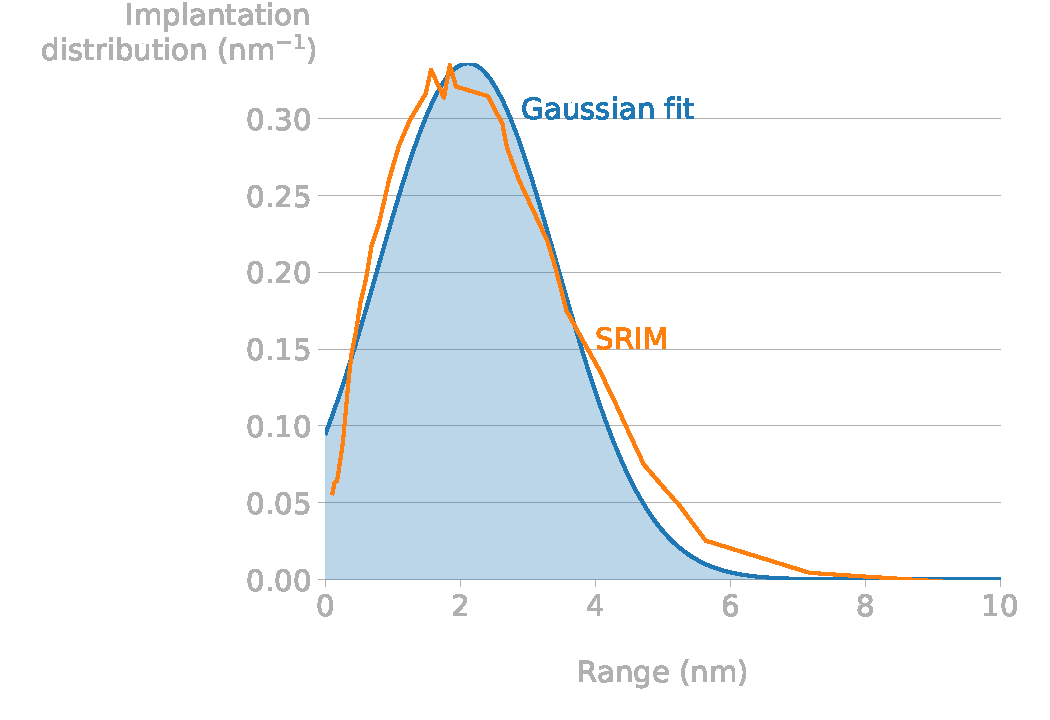
\includegraphics[width=\linewidth]{Figures/Chapter1/srim_implantation_range.pdf}
    \caption{\SI{100}{eV} deuterium implantation profile in tungsten computed from \gls{srim}. Reproduced from \cite{shimada_improved_2019}.}
    \labfig{srim_implantation_profile_example}
\end{figure}

% In order to accurately model this source term, the size of the cells constituing the mesh (the spatial discretisation of the domain) must be less than a nanometre.
% This can be done easily in 1D but is very complicated in higher dimensions, especially when simulating centimetre-sized components.
This volumetric source term can be simplified into a Dirichlet boundary condition (i.e.\ enforcing the mobile particle concentration at the exposed surface).

Let us consider a volumetric source term of hydrogen $\Gamma = \varphi_\mathrm{imp} \; f(x)$ where $f$ is a narrow Gaussian distribution.
The concentration profile of mobile particles can be approximated by a triangular shape \sidecite{schmid_diffusion-trapping_2016} (see \reffig{recomb sketch}).

\begin{figure*}[h!]
    \centering
    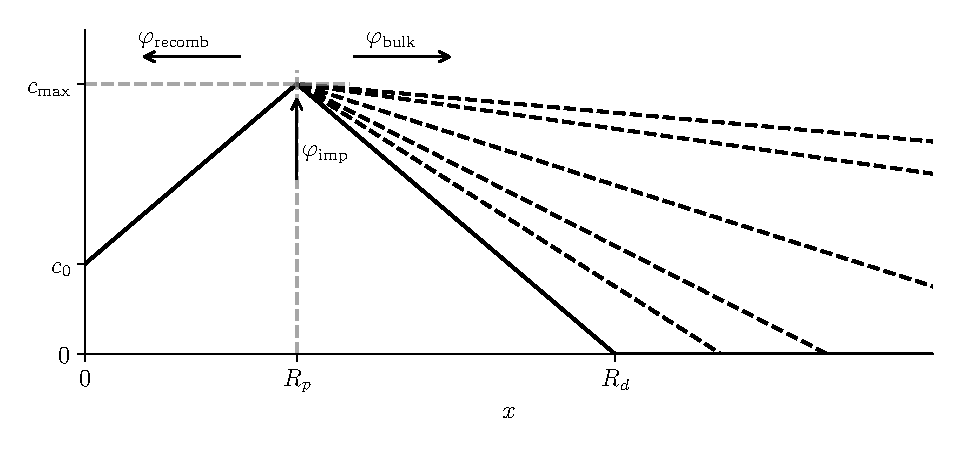
\includegraphics[width=0.75\linewidth]{Figures/Chapter2/recomb_sketch.pdf}
    \caption{Concentration profile with recombination flux and volumetric source term at $x=R_p$. Dashed lines correspond to the time evolution.}
    \labfig{recomb sketch}
\end{figure*}

The concentration profile is therefore maximum at $x=R_p$.
The expression of $c_\mathrm{max}$ can be obtained by expressing the flux balance at equilibrium:

\begin{equation}
    \varphi_\mathrm{imp} = \varphi_\mathrm{recomb} + \varphi_\mathrm{bulk}
    \labeq{flux balance}
\end{equation}
where $\varphi_\mathrm{recomb}$ is the recombination flux and $\varphi_\mathrm{bulk}$ is the migration flux.

$\varphi_\mathrm{bulk}$ can be expressed as:
\begin{equation}
    \varphi_\mathrm{bulk} = D \cdot \frac{c_\mathrm{max}}{R_d(t) - R_p}
\end{equation}
with $R_d$ the diffusion depth.

% When $t \rightarrow \infty$ or $R_d \gg R_p$ (a ratio of 10 or 100 is enough), $\varphi_\mathrm{bulk} \ll \varphi_\mathrm{recomb}$.
When $R_d \gg R_p$, $\varphi_\mathrm{bulk} \rightarrow 0$.
\refeq{flux balance} can therefore be written as:
\begin{equation}
    \varphi_\mathrm{recomb} \approx \varphi_\mathrm{imp}
    \labeq{flux balance 2}
\end{equation}

Moreover, according to Fick's law, $\varphi_\mathrm{recomb}$ can be expressed as:

\begin{align}
    \varphi_\mathrm{recomb} &= D \cdot \frac{c_\mathrm{max}-c_{0}}{R_{p}} = \varphi_\mathrm{imp}\\
    \Leftrightarrow c_\mathrm{max} &= \frac{\varphi_\mathrm{imp} R_{p}}{D}+ c_0
    \labeq{c_max}
\end{align}

Assuming second order recombination, $\varphi_\mathrm{recomb}$ can also be expressed as a function of the recombination coefficient $K_r$:

\begin{align}
    \varphi_\mathrm{recomb} &= K_r c_{0}^{2} = \varphi_\mathrm{imp}\\
    \Leftrightarrow c_{0} &= \sqrt{\frac{\varphi_\mathrm{imp}}{K_r}}
    \labeq{c_0}
\end{align}

By replacing \refeq{c_0} in \refeq{c_max} one can obtain:

\begin{equation}
    c_\mathrm{max} = \frac{\varphi_\mathrm{imp} R_{p}}{D}+\sqrt{\frac{\varphi_\mathrm{imp}}{K_r}}
\end{equation}

As the recombination process becomes fast (i.e.\ $K_r \rightarrow \infty$), $c_0 \rightarrow 0$ and $c_\mathrm{max} \rightarrow \frac{\varphi_\mathrm{imp} R_{p}}{D}$.

Since the main driver for the diffusion is the value $c_\mathrm{max}$, when $R_p$ is negligible compared to the dimension of the simulation domain, one can simply impose this value at the surface.
% This analytical simplification is especially useful to simulate implanted sources near the surface (e.g.\ plasma implantation) without having to finely discretise the domain to fully represent the gaussian distribution.
% Such a discretisation can be easily done for 1D simulations but is very complex in 2D and 3D and often makes the mesh very large which increases drastically the computational cost.

A transient solution based on trap properties can be derived \sidecite{hodille_study_2016}:
\begin{equation}
    c_\mathrm{max}(t)=\left( \frac{R_p \varphi_\mathrm{imp}}{D} + \sqrt{\frac{\varphi_\mathrm{imp}}{K_r}} \right) \cdot \frac{\tau}{t} \cdot\left(\sqrt{1+\frac{t}{\tau}}-1\right)^2
\end{equation}
where $\tau$ is a characteristic time expressed by:
\begin{equation}
    \tau = \frac{R_p \sum R_i \, n_i}{8 \varphi_\mathrm{imp}}
\end{equation}
In this expression, $R_i = (p / (k c_\mathrm{max}) + 1)^{-1}$ represents the maximum filling ratio of the trap $i$ and $n_i$ is the trap density.
When $t \gg \tau$, $c_\mathrm{max}(t) \approx \frac{R_p \varphi_\mathrm{imp}}{D} + \sqrt{\frac{\varphi_\mathrm{imp}}{K_r}}$

\subsection{Interface condition: conservation of chemical potential}\labsec{conservation of chemical potential}
% According to Krom \textit{et al} \sidecite{krom_hydrogen_2000}, since the solubility of hydrogen atoms in solids is low, the chemical potential of solute hydrogen $\mu$ is expressed by:
% \begin{equation}
%     \mu = \mu_0 + RT \ln\left( \frac{c_\mathrm{m}}{N_L}\right)
% \end{equation}
% where $\mu_0$ is the chemical potential in a reference state in \si{J.mol^{-1}}, $R$ the ideal gas constant, $T$ the temperature in \si{K}, $c_\mathrm{m}$ the mobile hydrogen concentration in \si{m^{-3}} and $N_L$ the lattice site concentration in \si{m^{-3}}.

% % Assuming that only free hydrogen atoms contribute to the overall flux in the material, the particle flux $J$ in \si{m^{-2}.s^{-1}} can be expressed by Fick's law:
% % \begin{equation}
% %     J = - D \nabla c_\mathrm{m}
% % \end{equation}
% % where $D$ is the diffusion coefficient of hydrogen expressed in \si{m^{2}.s^{-1}}. 


% The local equilibrium at the interface between two materials must ensure  the continuity of both the chemical potential $\mu$ (see \refeq{muconservation}) and the particle flux (see \refeq{flux conservation}).
% \begin{equation}
%     \mu^- = \mu^+  \labeq{muconservation}  
% \end{equation}
    
% \begin{equation}
%     D^- \nabla c_\mathrm{m}^- = D^+ \nabla c_\mathrm{m}^+ \labeq{flux conservation} 
% \end{equation}


% This assumption is correct as long as the time needed to reach the equilibrium is low compared to the time of the simulation.
% For long exposure time as well as for high temperatures, the characteristic time is small enough for the equilibrium model to be valid (see page \refpage{Interface transient model}).

% From \refeq{c/s conservation}, one can deduce that a solubility discontinuity across an interface induces a discontinuity of mobile hydrogen concentration $c_\mathrm{m}$.
% This can also be interpreted as the chemical potentials at a reference state being different in different materials \sidecite{kirchheim_25_2014}, as the lattice site concentration.

The continuity of chemical potential can be ensured by performing a change of variable in Fick's second law of diffusion with $\phi = c_\mathrm{m}/S$ (in the case of a metal) \sidecite{smith_abaqusstandard_2009} when internal conditions cannot be set.
Neglecting the trapping and generation terms, \refeq{mobile} therefore reads:

\begin{align}
    \frac{\partial \phi S}{\partial t} &= \nabla \cdot\left(D \nabla \phi S\right) + f \nonumber \\
    &=\nabla \cdot\left( D S \nabla \phi + D \phi \nabla S\right) + f \labeq{diffusion equation changed}
\end{align}

% Because $\phi$ is computed, the ratio $c_\mathrm{m}/S$ is continuous by default at the material interfaces.

% This second approach is used for instance in the \textit{mass-diffusion} procedure of the Abaqus code \sidecite{smith_abaqusstandard_2009}.
% This interface model has also been implemented into the current hydrogen transport code FESTIM \sidecite{delaporte-mathurin_finite_2019} using FEniCS \sidecite{alnaes_fenics_2015}.

After solving \refeq{diffusion equation changed} for $\phi$, $c_m$ can be retrieved by multiplying the solution by $S$.

\section{Heat transfer}
Due to the numerous processes that are thermally activated, it is essential to have an accurate temperature field.
Moreover, most tokamak plasma facing components are exposed to intense heat fluxes and are actively cooled, exhibiting high temperature gradients.
The temperature fields are even more complex when dealing with non-trivial geometries like monoblocks or breeding blankets.
For these reasons, heat transfers need to be modelled.

The equation describing heat conduction in solids is described as follows:
\begin{equation}
    \rho \cdot C_p \frac{\partial T}{\partial t}=\nabla \cdot (\lambda \nabla T)
    \labeq{heat equation}
\end{equation}
where $\rho$ is the density of the material in \si{kg.m^{-3}}, $C_p$ its specific heat capacity expressed in \si{J.kg^{-1}.K^{-1}} and $\lambda$ the thermal conductivity expressed in \si{W.m^{-1}.K^{-1}}.

The thermal properties $C_p$, $\rho$ and $\lambda$ are usually temperature dependent.

For heat transfer problems, three types of boundary conditions can be imposed.

First, the temperature can be fixed on the boundary with a Dirichlet boundary condition (see \refeq{dirichlet bc T}).
\begin{equation}
    T = T(x, y, z, t) \quad \text { on } \partial \Omega
    \labeq{dirichlet bc T}
\end{equation}
where $\partial \Omega$ is the domain boundary.

On the other hand, a heat flux can also be imposed by enforcing the temperature gradient (see \refeq{neumann bc T}).
This condition is called a Neumann condition.
\begin{equation}
    -\lambda \nabla T \cdot \mathbf{n} = f(x, y, z, t) \quad \text { on } \partial \Omega
    \labeq{neumann bc T}
\end{equation}
where $\lambda$ is the thermal conductivity in \si{W.m^{-1}.K^{-1}}, $\mathbf{n}$ is the boundary normal vector and $\partial \Omega$ is the domain boundary.

Finally, to model a convective heat flux when the surface is in contact with a fluid (e.g.\ cooling pipes, natural convection...), a Robin boundary condition needs to be employed (see \refeq{convective bc T}).
\begin{equation}
    -\lambda \nabla T \cdot \mathbf{n} = h (T - T_\mathrm{ext}) \quad \text { on } \partial \Omega
    \labeq{convective bc T}
\end{equation}
where $h$ is the heat transfer coefficient in \si{W.m^{-2}.K^{-1}}, $T_\mathrm{ext}$ is the fluid temperature in \si{K} and $\partial \Omega$ is the domain boundary.
The heat transfer coefficient can be dependent on the temperature and the flow characteristics.
It is obtained by computing the Nusselt number from correlations linking it to the Reynolds number of the flow and the Prandtl number of the fluid \sidecite{poirier_correlations_2016} (e.g.\ Dittus-Boetler, Sieder-State, Gnielinski...).
Once the Nusselt number is known, the heat transfer coefficient $h$ reads:
\begin{equation}
    h = \frac{\lambda \, \textit{Nu}}{L}
\end{equation}
with $\lambda$ the thermal conductivity of the fluid in \si{W.m^{-1}.K^{-1}}, $\textit{Nu}$ the Nusselt number and $L$ the characteristic length in \si{m}.


\section{Implementation}


The models described in this Section can be hard to solve analytically for complex problems (complex geometries, transients, combined boundary conditions, etc.).
The code \gls{festim} \sidecite{delaporte-mathurin_finite_2019} was therefore developed in order to numerically solve these coupled equations.

\subsection{The finite element method: FEniCS}
\gls{festim} is based on the Finite Element Method to solve this set of differential equations and boundary conditions.
Several finite element libraries are available open-source (deal.II \sidecite{arndt_dealii_2021}, MFEM \sidecite{kolev_tzanio_modular_2010}, MOOSE \sidecite{permann_moose_2020}, FreeFEM++ \sidecite{hecht_new_2012}...).
The open-source python/C++ package \gls{fenics} \sidecite{alnaes_fenics_2015} was employed.
The finite element method is a versatile tool that can solve any partial differential equation on an arbitrary geometry in 1D, 2D or 3D.
The main advantage of this method compared to the finite difference method is the simplicity of its application to complex geometries and unstructured meshes.
Indeed, implementing a finite difference scheme for such a problem would be tedious and extra care must be taken for mistakes in the implementation could result in losses in efficiency and accuracy of the numerical solution.

This section illustrates the finite element method applied to Poisson's equation \sidecite{logg_automated_2012}.

The mathematical problem can be described by \refeq{example poisson} where $u$ is the unknown to be solved governed by Poisson's equation.
The problem is constrained by boundary conditions defined on $\partial \Omega$, the boundary of the domain.
The value of $u$ is prescribed on the subset $\Gamma_D$ (Dirichlet boundary condition) whereas the value of the normal derivative of $u$ is prescribed on the remaining boundary $\Gamma_N$ (Neumann boundary condition) (see \reffig{fe problem sketch}).

\begin{subequations}
    \begin{align}
        -\nabla^2 u &= f \quad \text{on    } \Omega \\
        u &= u_0 \quad \text{on    } \Gamma_D  \subset \delta \Omega \\
        -\frac{\partial u}{\partial n} &= g \quad \text{on    } \Gamma_N  \subset \delta \Omega
    \end{align}
    \labeq{example poisson}
\end{subequations}


\begin{figure} [h]
    \centering
    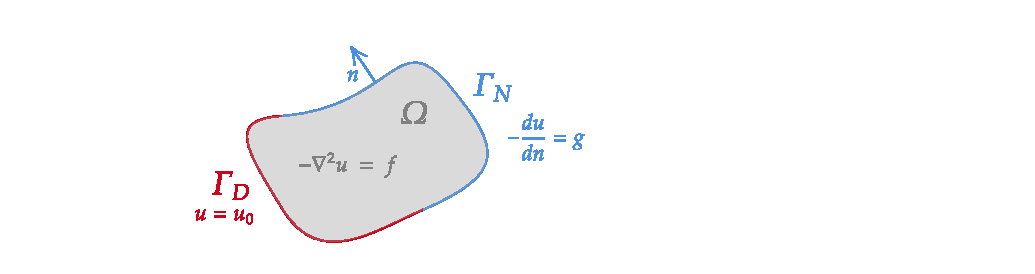
\includegraphics[trim=50 0 200 0, clip, width=0.7\linewidth]{Figures/Chapter2/finite_element_problem_sketch.pdf}
    \caption{Representation of the mathematical problem.}
    \labfig{fe problem sketch}
\end{figure}

The first step of the finite element method is to build a variational formulation (also called \textit{weak form}) of the governing \refeq{example poisson} (called the \textit{strong form}).
To do so, the equation is multiplied by a function $v$ (called the \textit{test function}) and integrated over the domain $\Omega$.
The following expression is obtained:
\begin{equation}
    \int_{\Omega} -\nabla^2 \ u \ v \ dx = \int_{\Omega} f \ v \ dx \quad \forall \ v \in \hat{V}
    \labeq{weak form 1}
\end{equation}

The function space $\hat{V}$ is defined as:
\begin{equation}
    \hat{V} = \{ v \in H^1(\Omega) \ : \ v=0 \ \text{on} \ \Gamma_D \}
\end{equation}

\refeq{weak form 1} needs now to be rewritten in order to only have first order derivatives.
To do so, Gauss-Green's lemma is employed:
\begin{equation}
    \int_{\Omega} -\nabla^2 u \ v \ dx = \int_{\Omega} \nabla u \cdot \nabla \ v \ dx - \int_{\partial \Omega} \frac{\partial u}{\partial n} \ v \ ds
    \labeq{gauss-green}
\end{equation}

Since the test function $v$ vanishes on $\Gamma_D$, the following variational problem is obtained: find $u \in V$ such that
\begin{equation}
    \int_{\Omega} \nabla u \cdot \nabla v  \ dx = \int_{\Omega} f \ v \ dx - \int_{\Gamma_N} g \ v \ ds \quad \forall \ v \in \hat{V}
    \labeq{weak form 2}
\end{equation}

The function space $V$ is defined as:
\begin{equation}
    V = \{ v \in H^1(\Omega) \ : \ v=u_0 \ \text{on} \ \Gamma_D \}
\end{equation}

Poisson's equation can now be discretised by restricting the variational problem \refeq{weak form 2} to discrete function spaces $V_h$ and $\hat{V}_h$: find $u_h \in V_h \subset V$
\begin{equation}
    \int_{\Omega} \nabla u_h \cdot \nabla v  \ dx = \int_{\Omega} f \ v \ dx - \int_{\Gamma_N} g \ v \ ds \quad \forall \ v \in \hat{V}_h \subset \hat{V}
    \labeq{discrete variational problem}
\end{equation}

To solve \refeq{discrete variational problem}, a suitable pair of discrete function spaces $V_h$ and $\hat{V}_h$ must be constructed.
Piecewise polynomial basis functions $\{ \phi_i \}_{i=1}^N$ are defined for $V_h$ and $\{ \hat{\phi}_j \}_{j=1}^N$ for $\hat{V}_h$.

The approximated solution $u_h$ therefore reads (see \reffig{example approximated solution}):
\begin{equation}
    u_h(x) = \sum^N_{i=1}U_i \phi_i(x)
    \labeq{FEM solution}
\end{equation}
where $U_i$ are the coefficient to be determined on each node (called degrees of freedom).
$N$ is the number of nodes used to discretise the domain.

\begin{figure}
    \centering
    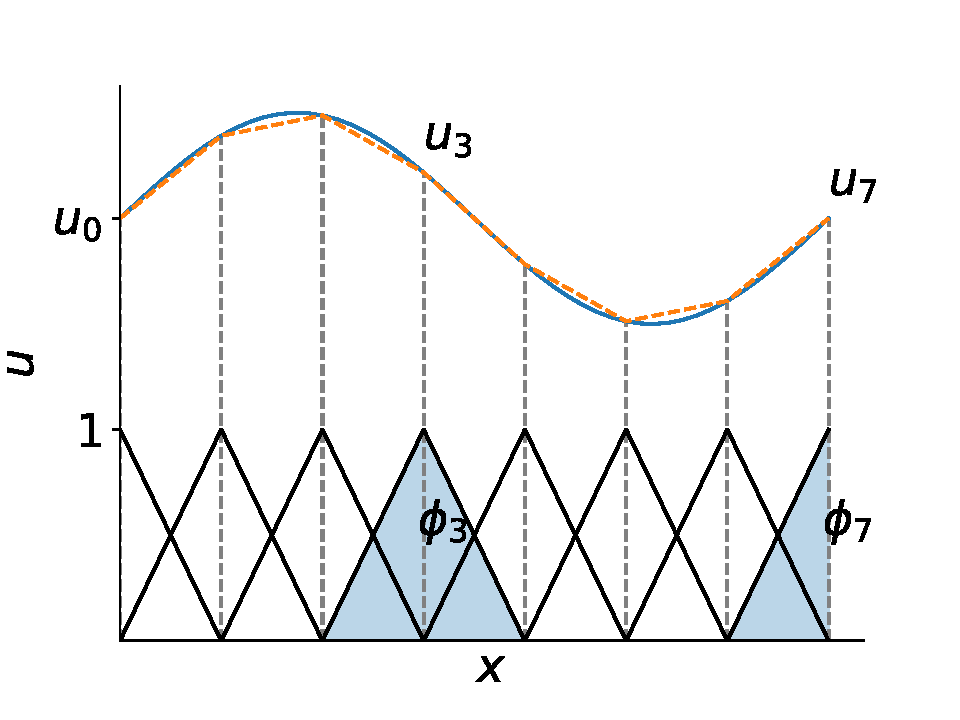
\includegraphics[width=\linewidth]{Figures/Chapter2/approximated_solution.pdf}
    \caption{1D example of an approximated solution $u$ (exact in blue, approximated in orange) with basis function $\phi_i$ for linear finite elements with 2 nodes.}
    \labfig{example approximated solution}
\end{figure}

By replacing $u_h$ in \refeq{discrete variational problem} with \refeq{FEM solution} and varying the basis functions $\hat{\phi}_j$:

\begin{equation}
    \sum^N_{i=1} U_i \int_\Omega \nabla \phi_i \cdot \nabla \hat{\phi}_j \ dx = \int_\Omega f \ \hat{\phi}_j \ dx - \int_{\Gamma_N} g \ \hat{\phi}_j \ ds , \quad \ j = 1, \ 2, \ \ldots, \ N
\end{equation}

This can be written in a matrix form:
\begin{equation}
    AU = b
    \labeq{variational problem matrix form}
\end{equation}
where
\begin{subequations}
    \begin{align}
        A_{ji} &= \int_\Omega \nabla \phi_i \cdot \nabla \hat{\phi}_j \ dx \\
        b_{j} &= \int_\Omega f \ \hat{\phi}_j \ dx - \int_{\Gamma_N} g \ \hat{\phi}_j \ ds
    \end{align}
    \labeq{eq: matrices A and b}
\end{subequations}

The integral terms in \refeq{eq: matrices A and b} are computed with Gauss-Legendre quadrature.

After solving \refeq{variational problem matrix form}, the $U_i$ coefficients are known and the approximated solution $u_h$ can be computed.
Non-linear problems are solved similarly where the solution is approached using Newton's method.

\subsection{Main features of \gls{festim}}
\gls{festim} provides an even higher level of abstraction than \gls{fenics} by providing a user-friendly interface dedicated to H transport and heat transfer problems.
Users only have to provide inputs such as material properties, traps properties, geometry, solving parameters, without having to dive into the finite element implementation.
In other words, users do not need to be finite element experts to run a \gls{festim} simulation (though knowledge and experience in finite elements will help in solving numerical problems).

% user friendly
Multidimensional multi-material transient simulations coupled with heat transfer can therefore be run fairly easily without finite element knowledge.
Nevertheless, since \gls{festim} is object-oriented, advanced users will always be able to turn \gls{festim} inside-out to adapt the code to their specific needs (specific boundary conditions, slight changes in the governing equations...).
Since \gls{festim} is written in python - which is a fairly easy-to-learn programming language - no advanced level of coding is required.

% physics
As mentioned above, \gls{festim} simulates hydrogen transport (diffusion and trapping) and additional physics can be incorporated, such as the Soret effect (even though not used in this work) and conservation of chemical potential at interfaces...
The hydrogen transport equations can be coupled to the heat equation (weak coupling).
Various types of boundary conditions are available for both the H transport (imposed concentration, recombination flux, dissociation flux, implanted source approximation...) and the heat transfer problems (imposed temperature, imposed flux, convective flux...).
Traps densities in FESTIM can also be time-dependent allowing the users to simulate extrinsic traps (e.g.\ irradiation induced traps, stress induced traps...).

% geometry
Thanks to the finite element method, geometries used in \gls{festim} can be complex (see \reffig{example mesh}).
The meshing capability of \gls{festim} is limited to 1D meshes, and it was decided to instead make \gls{festim} accept (with the XDMF format) complex meshes from third-party applications dedicated to meshing such as SALOME or GMSH.
These third-party applications can for instance be useful to run CAD-based simulations.
Users can also decide to use the \gls{fenics} built-in meshing tool.

\begin{figure}
    \centering
    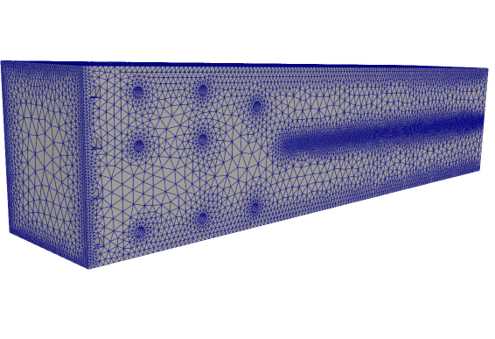
\includegraphics[width=0.5\linewidth]{Figures/Chapter2/example_mesh.png}
    \caption{Example of a complex 3D geometry (here a breeding blanket section) mesh readable by \gls{festim} \cite{dark_influence_2021}.}
    \labfig{example mesh}
\end{figure}

% visualisation
Similarly, \gls{festim} (\gls{fenics}) visualisation functions are limited.
\gls{festim} is not a graphical application, but the files generated by \gls{festim} (XDMF, CSV, TXT) can easily be read and post-processed by specialised tools such as Paraview \sidecite{ahrens_paraview_2005}, matplotlib \sidecite{hunter_matplotlib_2007}, NumPy \sidecite{harris_array_2020}, etc.

% what FE
Regarding the default finite elements used in \gls{festim} are first order piecewise elements (called P1, Lagrange or also Continuous Galerkin 1).
Using these finite elements for trapped concentration exhibiting discontinuities (at the interface between two materials for instance) can cause performance issues and loss of accuracies.
Therefore, it can be switched to discontinuous elements (DG1) when needed to avoid under- or over-shoots in the concentration fields.
Many different finite elements are available in \gls{fenics} \cite{noauthor_periodic_nodate} and their description is outside the scope of this work.

% Adaptive step size
When dealing with transient problems, \gls{festim} provides an adaptive stepsize allowing the stepsize to increase (by a user-defined factor) when the convergence criterion is easily reached by the solver.
This greatly improves the performance of the code since less timesteps are needed.



\section{Verification \& Validation}

Before using the \gls{festim} code for analysis, it has to be verified and validated.
The \gls{vv} has two goals: (1) to prove that the governing equations are correctly solved and that the code is error free and (2) to demonstrate that the governing equations actually reproduce processes observed experimentally.
In other words, verification is answering the question \textit{``Are we building the code right?''} and validation is answering the question \textit{``Are we building the right code?''}.

This Section details the \gls{vv} of \gls{festim}.

\subsection{Analytical verification}
Verification is the process of ensuring the governing equations are correctly solved in FESTIM.
This is an integral part of every simulation code for it guarantees the code is error free.
It is generally hard to simply substitute this process by code comparison (cross-checks between two different codes) because often the codes are implemented differently.
Moreover, if the code we are comparing with is not verified, then obtaining similar results does not give any guarantee on the code accuracy as two different codes can have the same bug.

Several methods can be used to verify a code but the \gls{mes} and the \gls{mms} are employed here.

Both methods consist in comparing a computed solution with an exact solution and measuring the error.
The exact solution in the \gls{mes} is obtained by solving the governing equations analytically.
When using the \gls{mms}, the problem is reversed: an arbitrary exact solution (called \textit{manufactured solution}) is chosen and injected in the governing equations.
It is then possible to determine source terms and boundary conditions.
These are then fed into the code and the computed solution is compared to the manufactured (exact) solution.

This \gls{mms} is often used to unravel the complexity of governing equations \sidecite{dudson_verification_2016, roache_code_2002}.
This is particularly useful when dealing with complex geometries or to exercise non-trivial material properties.

This section describes two verification cases of \gls{festim}.
The first one uses the \gls{mes} and the second one the \gls{mms}.
More complex and thorough verification cases are shown in Appendix \ref{appendix verification}.

\subsubsection{Case 1: H transport (\gls{mes})} \labsec{analytical}

\begin{figure}
    \centering
    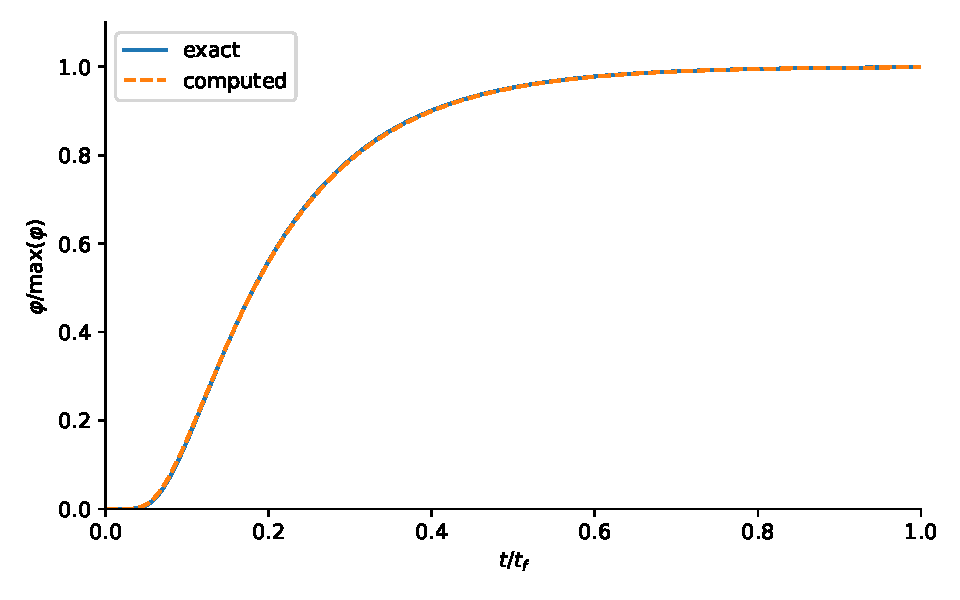
\includegraphics[width=\linewidth]{Figures/Chapter3/mes_festim_effective_diffusion.pdf}
    \caption{Temporal evolution of the outward particle flux $\varphi$ at $x=l$ (Case 1).}
    \labfig{FESTIM vs analytical}
\end{figure}

% Although validation against experiments could show that FESTIM is able reproduce the data with a given set of parameters, objective verification against analytical solutions is first required to ensure that the governing \refeq{mobile} and \refeq{trapped} are solved correctly.

For this verification case, a 1D slab is considered with a thickness $l$.
The concentration of mobile particles was set to $c_0$ on one side of the slab and set to zero on the other side.
Only one trap is considered in this case and its density $n$ is homogeneously distributed.

The trapping parameter $\zeta$ is defined in \sidecite{longhurst_verification_2005} as follows:
\begin{equation}
    \zeta = \frac{p}{k \: n} + \frac{c_\mathrm{m}}{n}
\end{equation}

In our case, we choose the trapping and detrapping rates $k$ and $p$, the concentration $c_0$ and the temperature $T$ so that $\zeta \gg \frac{c_\mathrm{m}}{n}$.
This condition is equivalent to having the trap filling ratio $(p / (k \, c_\mathrm{m}) + 1)^{-1} \ll 1$.
This is known as the \textit{effective diffusivity regime} where the diffusion is almost identical to the case where there are no traps.
In this regime, the governing equations are identical as a pure diffusion regime and are therefore easy to solve analytically.

The coefficient $D$ is then replaced by an effective diffusion coefficient:
\begin{equation}
    D_\mathrm{eff} = \frac{D}{1+\frac{1}{\zeta}}
\end{equation}
The particle flux at the background surface ($x=l$) is expressed in $\si{H.m^{-2}.s^{-1}}$ and finally defined in \cite{longhurst_verification_2005} by:
\begin{equation}
    \varphi(t) = \frac{c_0 D}{l}\bigg[1+2\sum_{m=1}^{\infty}(-1)^m \exp\bigg(-m^2\frac{\pi^2 \:D_\mathrm{eff} \: t}{l^2}\bigg)\bigg]
\labeq{flux analytical}
\end{equation}
In \refeq{flux analytical}, the infinite sum has been truncated at $m=10000$.

All the parameters used in this verification case are defined in \reftab{parameters analytical verification}.
These parameters have been chosen for the sake of verification and do not necessarily represent realistic conditions as verification is a mathematical exercise.
\begin{table}
    \centering
    \begin{tabular}{p{2.3cm} p{2cm} r}
        Parameter & Units & Value \\
        \hline
        \\
        $D_0$ & $\si{m^2.s^{-1}}$ & 2.0 \\
        $k_0$ & $\si{m^3.s^{-1}}$ & 0.01 \\
        $p_0$ & $\si{s^{-1}}$ & 1.0 \\
        \\
        $E_D$ & $\si{eV}$ & 0.2 \\
        $E_k$ & $\si{eV}$ & 0.1 \\
        $E_p$ & $\si{eV}$ & 0.1 \\
        \\
        $c_0$ & $\si{m^{-3}}$ & 2.0 \\
        $n$ & $\si{m^{-3}}$ & 2.0 \\
        $l$ & $\si{m}$ & 1.5\\
        \\
        $T$ & $\si{K}$ & 300 \\
        \\
        $t_f$ & $\si{s}$ & 2000 \\
        \\
    \end{tabular}
    \caption{Parameters used for the analytical verification (Case 1).}
    \labtab{parameters analytical verification}
\end{table}
One can notice on \reffig{FESTIM vs analytical} that the numerical results are in good agreement with the analytical solution.
The relative L2 error between analytical and numerical solutions was found to be $\approx 1 \%$ with 1000 piecewise linear elements (\gls{p1}) and a stepsize of \SI{1}{s}.
This value decreases with the stepsize and with the element size (see \reffig{MES evolution of L2 error as function of dt and dx}).
\begin{figure}
    \centering
    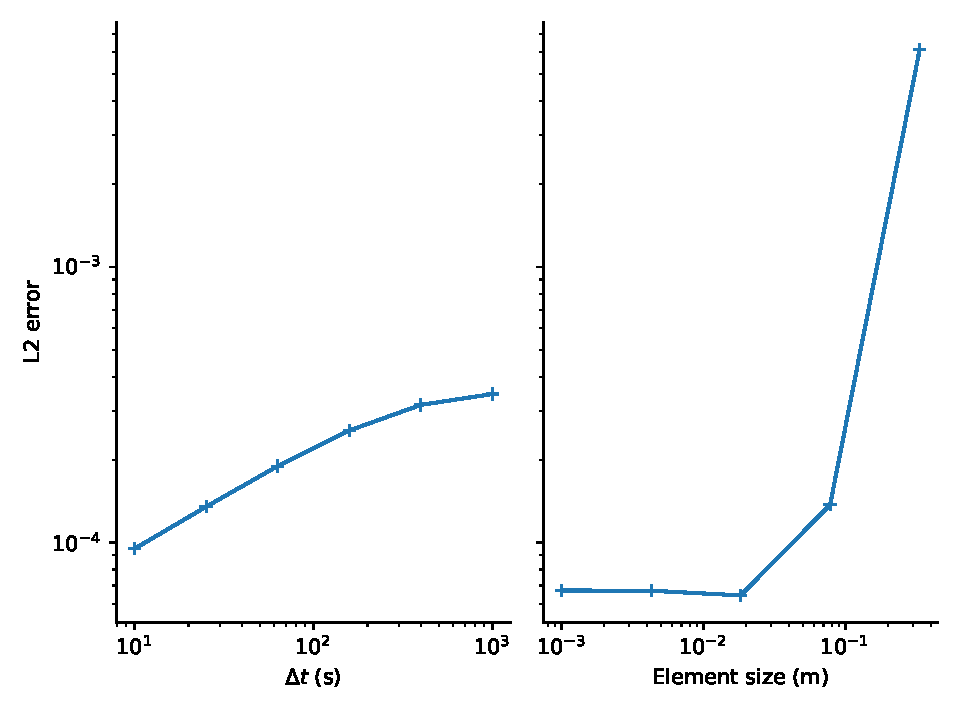
\includegraphics[width=\linewidth]{Figures/Chapter2/error_vs_element_size_and_dt.pdf}
    \caption{Evolution of the L2 error on $\varphi$ as a function of the stepsize and element length (Case 1).}
    \labfig{MES evolution of L2 error as function of dt and dx}
\end{figure}


Since this test case is very similar to a pure diffusion case, it does not exercise all terms of the governing equations.
To do so, the governing equations would have to be solved for a generic case which proves to be complex.
This is why the \gls{mms} will be used instead.

\subsubsection{Case 2: H transport (\gls{mms})} \labsec{mms}

\paragraph{Principle}
The \gls{mms} is often used to unravel the complexity of governing equations \sidecite{dudson_verification_2016, roache_code_2002}.
This is particularly useful when dealing with complex geometries or to exercise non-trivial material properties.

The principle of the \gls{mms} is to manufacture an exact solution.
Again, physical realism is not a concern here as verification is a mathematical exercise.
This manufactured solution needs to be non-trivial in order to test the robustness of the implementation.
It is then passed through the governing equations (either the heat equation or the hydrogen transport equations) and source terms are obtained.

Let us take a simple example with the Poisson equation defined on a 1D domain $[x_1, x_2]$:
\begin{equation}
    \frac{\partial u}{\partial t} = \frac{\partial^2 u}{\partial x^2} + q
    \labeq{poisson eq demo mms}
\end{equation}
where $u$ is the unknown, $q$ is the source term.

The manufactured solution is arbitrarily defined as:
\begin{equation}
    U(t, x) = A + \sin{(x + B t)}
\end{equation}
where $A$ and $B$ are real numbers, $t$ is the time, and $x$ is the spatial coordinate.
By replacing $u$ by $U(t, x)$ in \refeq{poisson eq demo mms}, we can identify the source term $q$ that would produce the solution $U(t, x)$:

\begin{equation}
    Q(t, x) = B \cos{(x + B t)} + \sin{(x + B t)}
\end{equation}

Several boundary conditions can be used to produce $U(t, x)$.
We can for instance set a Dirichlet boundary condition on the boundaries $x=x_1$ and $x=x_2$:
\begin{align}
    u(t, x_1) &= U(t, x_1) \\
    u(t, x_2) &= U(t, x_2)
\end{align}

or Neumann boundary conditions:
\begin{align}
    \frac{\partial u(t, x)}{\partial x}\Big | _{ x=x_1} &= \frac{\partial U(t, x)}{\partial x} \Big | _{ x=x_1} \\
    \frac{\partial u(t, x)}{\partial x}\Big | _{ x=x_2} &= \frac{\partial U(t, x)}{\partial x} \Big | _{ x=x_2}
\end{align}

or even a combination of Dirichlet and Neumann boundary conditions.

By solving \refeq{poisson eq demo mms} with $q = Q(t, x)$ and initial condition $u = U(0, x)$, we can obtain the computed solution $u_\mathrm{computed}$.
The error between the computed solution $u_\mathrm{computed}$ and the exact solution $U(t, x)$ can be calculated to assess the code accuracy.

\paragraph{Case 2a: Application to 1D hydrogen transport}

Let us apply the \gls{mms} to the hydrogen transport model on a 1D domain $\Omega$.
In order to exercise all terms in \refeq{mobile} and \refeq{trapped}, the following manufactured solutions are chosen:
\begin{equation}
    \begin{cases}
    c_{m_D} = 1 + x^2 + \sin(t) \\
    c_{{t,1}_D} = 1 + x^2 + \cos(t)
    \end{cases}
    \labeq{manufactured solutions}
\end{equation}

By combining \refeq{mobile}, \refeq{trapped} and \refeq{manufactured solutions}, one can obtain the following source terms:
\begin{equation}
    \begin{cases}
    f = \cos(t) - \sin(t) - 2D \\
    g_1 = p_1 c_{{t,1}_D} - k_1 c_{m_D} ( n_1 - c_{{t,1}_D}) - \sin(t)
    \end{cases}
    \labeq{sources}
\end{equation}
$f$ is the source term of the mobile concentration equation and $g_1$ is the source term of the trapped concentration equation.

where $g_1$ is an additional source term in \refeq{trapped}.
The Dirichlet boundary conditions for $c_\mathrm{m}$ and $c_{t,1}$ are:

\begin{equation}
    \begin{cases}
    c_\mathrm{m} = 1 + x^2 + \sin(t) \quad \text{on } \partial \Omega \\
    c_{t,1} = 1 + x^2 + \cos(t) \quad \text{on } \partial \Omega 
    \end{cases}
\end{equation}
where $\partial\Omega$ is the boundary of the domain.
Finally, initial values for $c_\mathrm{m}$ and $c_{t,i}$ are:
\begin{equation}
    \begin{cases}
    c_\mathrm{m}(t=0) = 1 + x^2 \\
    c_{t,1}(t=0) = 2 + x^2
    \end{cases}
\end{equation}
Once all these parameters are fed into FESTIM, one can easily compare the computed solution with the exact solution in \refeq{manufactured solutions}.
The L2-norm $E_{c_\mathrm{m}}$ can then be calculated as follows:
\begin{equation}
    E_{c_\mathrm{m}} = \sqrt{\int_\Omega(c_{m_D} - c_\mathrm{m})^2dx}
\end{equation}
The evolution of $E_{c_\mathrm{m}}$ as function of the element size $h$ is shown on \reffig{error vs h}.
One can notice that $E_{c_\mathrm{m}}$ increases as $A\cdot h^k$.
This is known as the \textit{asymptotic regime} and the coefficient $k$ is called the convergence rate.
$k$ typically approaches $N+1$ as $h$ approaches zero, $N$ being the order of the finite elements.
In this case, $k \approx 2$ as expected since first order finite elements have been used.

\begin{figure}
    \centering
    \includegraphics[width=1\linewidth]{"Figures/Chapter3/L2 error on Cm vs h"}
    \caption{Evolution of the L2 norm of the error as function of element size h for the 1D H transport case (Case 2a).}
    \labfig{error vs h}
\end{figure}

\paragraph{Case 2b: Application to 2D hydrogen transport}


The same method can be applied to a 2D case.
Let us choose the following steady state test problem on a domain $\Omega = [0, 1] \times [0, 1]$ with the manufactured solution $c_D(x, y) = \sin(\omega \pi x) \sin(\omega \pi y)$.

\begin{align}
    \nabla \cdot D \nabla c_\mathrm{m} &= -f_1 \\
    k c_\mathrm{m} (n - c_\mathrm{t}) - p c_\mathrm{t} &= -f_2 \\
    c_\mathrm{m} &= c_\mathrm{t} = c_D \text{  on  } \partial \Omega \\
    D &= 2 \\
    p &= 3 \\
    k &= 2 \\
\end{align}

The source terms $f_1$ and $f_2$ and the boundary conditions can be obtained in a similar fashion by replacing $c_\mathrm{m}$ and $c_\mathrm{t}$ in the governing equations.

It was shown that the computed solutions was similar to the exact solutions (see \reffig{results MMS 2D H transport}).
Moreover, the convergence rates confirm the mesh dependency of the computed solutions' accuracy (see \reffig{convergence rates H}).
% A super-convergence is observed for the P2 elements.

\begin{figure*}
    \centering
    \begin{subfigure}{0.3\linewidth}
        \centering
        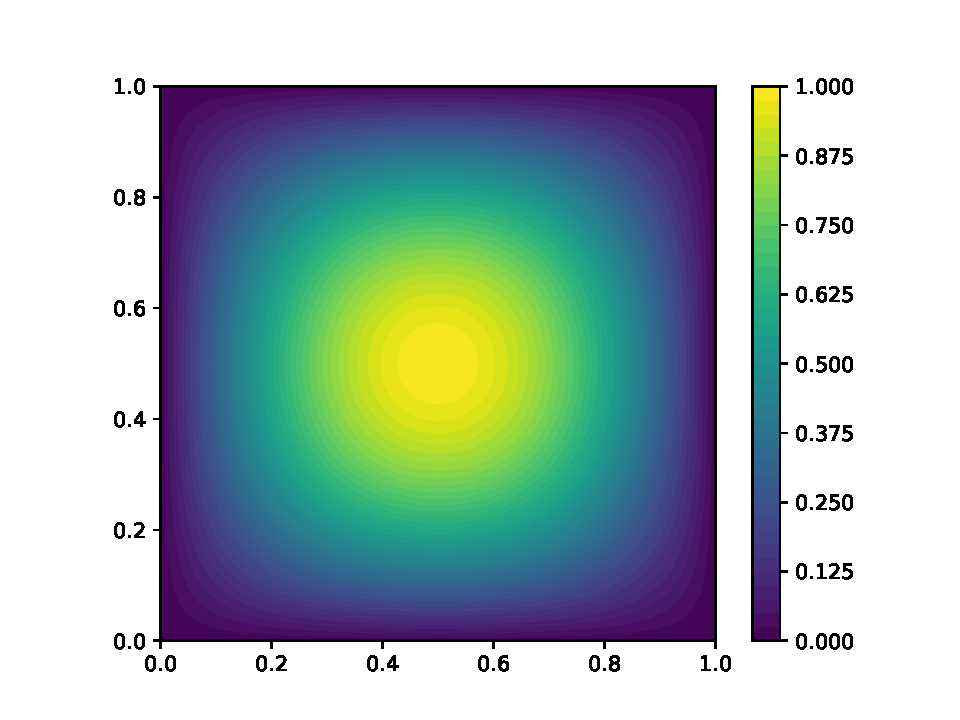
\includegraphics[width=\linewidth]{Figures/Chapter2/c_m.pdf}
        \caption{Computed $c_\mathrm{m}$ (64 elements).}
    \end{subfigure}%
    \begin{subfigure}{0.3\linewidth}
        \centering
        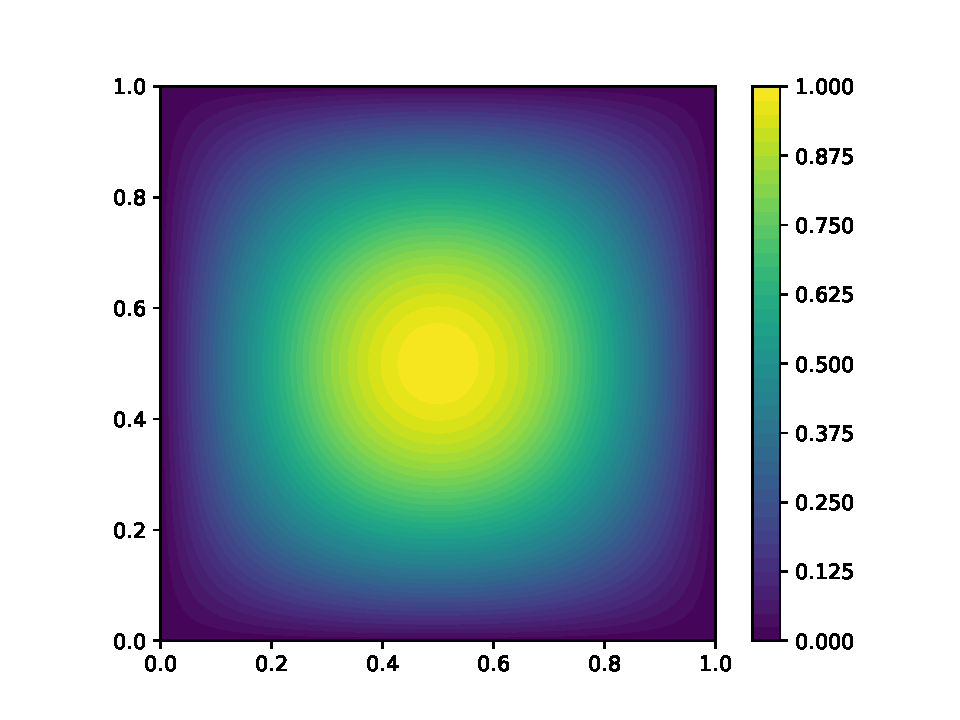
\includegraphics[width=\linewidth]{Figures/Chapter2/c_t.pdf}
        \caption{Computed $c_\mathrm{t}$ (64 elements).}
    \end{subfigure}%
    \begin{subfigure}{0.3\linewidth}
        \centering
        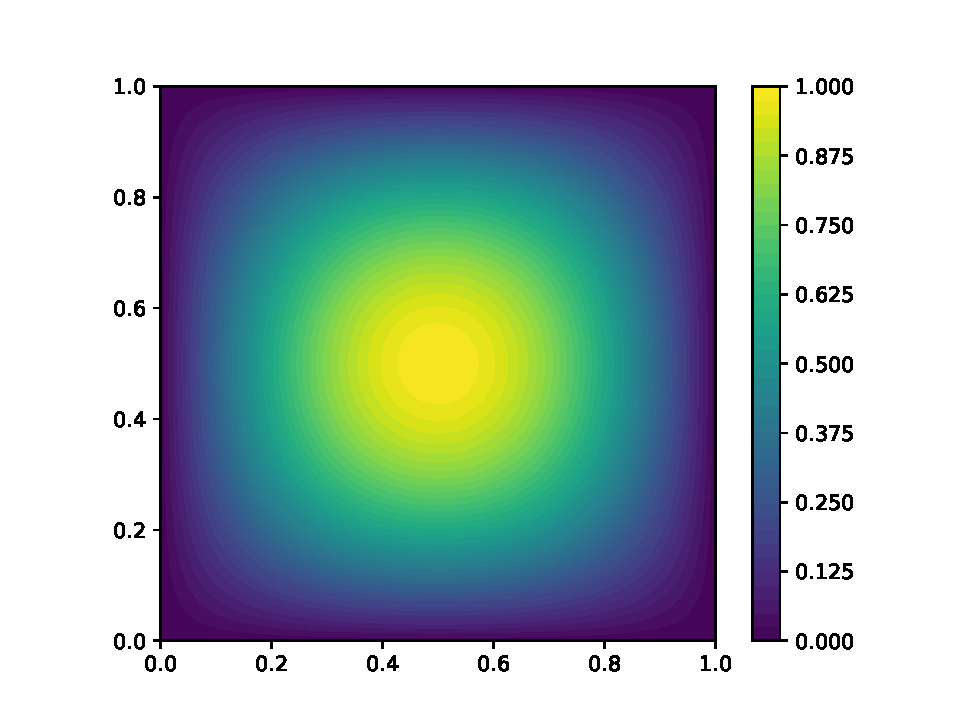
\includegraphics[width=\linewidth]{Figures/Chapter2/c_exact.pdf}
        \caption{Exact solution $c_D$.}
    \end{subfigure}
    \caption{Comparison of the computed concentrations with the exact solution (Case 2b).}
    \labfig{results MMS 2D H transport}
\end{figure*}

\begin{figure}
    \centering
    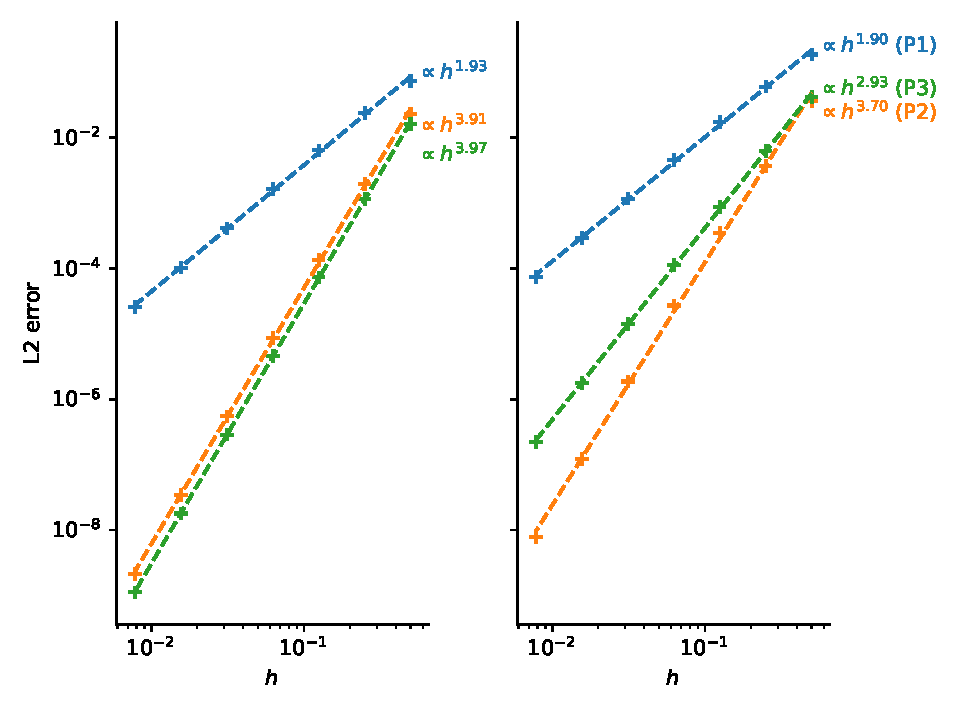
\includegraphics[width=\linewidth]{Figures/Chapter2/convergence_rate_H.pdf}
    \caption{Evolution of the L2 error on $c_\mathrm{m}$ (left) and $c_\mathrm{t}$ (right) showing the convergence rates for the 2D H transport case (Case 2b).}
    \labfig{convergence rates H}
\end{figure}



\subsection{Experimental validation}

Now that the code has been verified (\textit{ie} solves the governing equations correctly), experimental validation is still required to check that these equations actually represent real life processes.
A very good example of real life experiments that can be reproduced are Thermo-Desorption Spectroscopy (TDS) experiments also called Thermally Programmed Desorption (TPD) experiments.
The principle of such experiments is to load small samples with H isotopes (H, D, or T) - either with a gas infusion or via plasma implantation - and heat them up to different temperatures to desorb the trapped H.
By measuring the outgassing flux of particles throughout the time of the experiment, desorption spectra are obtained.
These spectra often exhibit several peaks and each peak correspond to a kind of trap.

This technique is therefore employed to characterise materials and determine their defects. 
It is also a very good application case for experimental validation of the H transport model.

This section describes the technique that was employed to easily reproduce these TDS experiments.
% Several application cases will also be shown on W, Al, EUROFER, and Be.

\subsubsection{Methodology} \label{methodology}
Fitting experimental data by manually tweaking parameters as in \sidecite{yu_deuterium_2019, hodille_macroscopic_2015} can be really time-consuming, sometimes days in some cases.
Moreover, some possible solutions in the parameter space might be missed by the user.
This process has been automated by embedding \gls{festim} in a minimisation algorithm.

As in manual fitting, the parametric optimisation problem is solved by minimising a function representing the residual between simulated results and some reference data.
This function $f$ is called \textit{cost function}.
Considering fitting one or several \gls{tds} spectra (in order to identify for instance trapping parameters or diffusion coefficients), $f$ can simply be the mean absolute error described in Equation \ref{eq:cost function} representing the residual between the simulated spectrum and the experimental reference: 

\begin{equation}
    f(\textbf{x})=\frac{\sum_{i=0}^{N}  \alpha_i(T_i)\left| d_{i}-d_{\mathrm{sim}}\right|}{\sum_{i=0}^{N}  \alpha_i(T_i)}
    \label{eq:cost function}
\end{equation}

where \textbf{x} is the set of parameters used for the simulation, $d_\mathrm{sim}$ are the values of the simulated spectrum, $N$ is the number of experimental points $(T_i, d_i)$.
In Equation \ref{eq:cost function}, $f(\textbf{x})$ can be weighted by coefficients $\alpha_i$ in order to have a better fit on specific regions of the spectrum.
%Note that this cost function could as well be a root mean square error or any type of residual.

The parametric optimisation problem can now be solved by finding the minimum of the cost function $f$.
The global optimisation routine is illustrated on Figure \ref{fig:diagramm}.
\begin{figure}
    \centering
    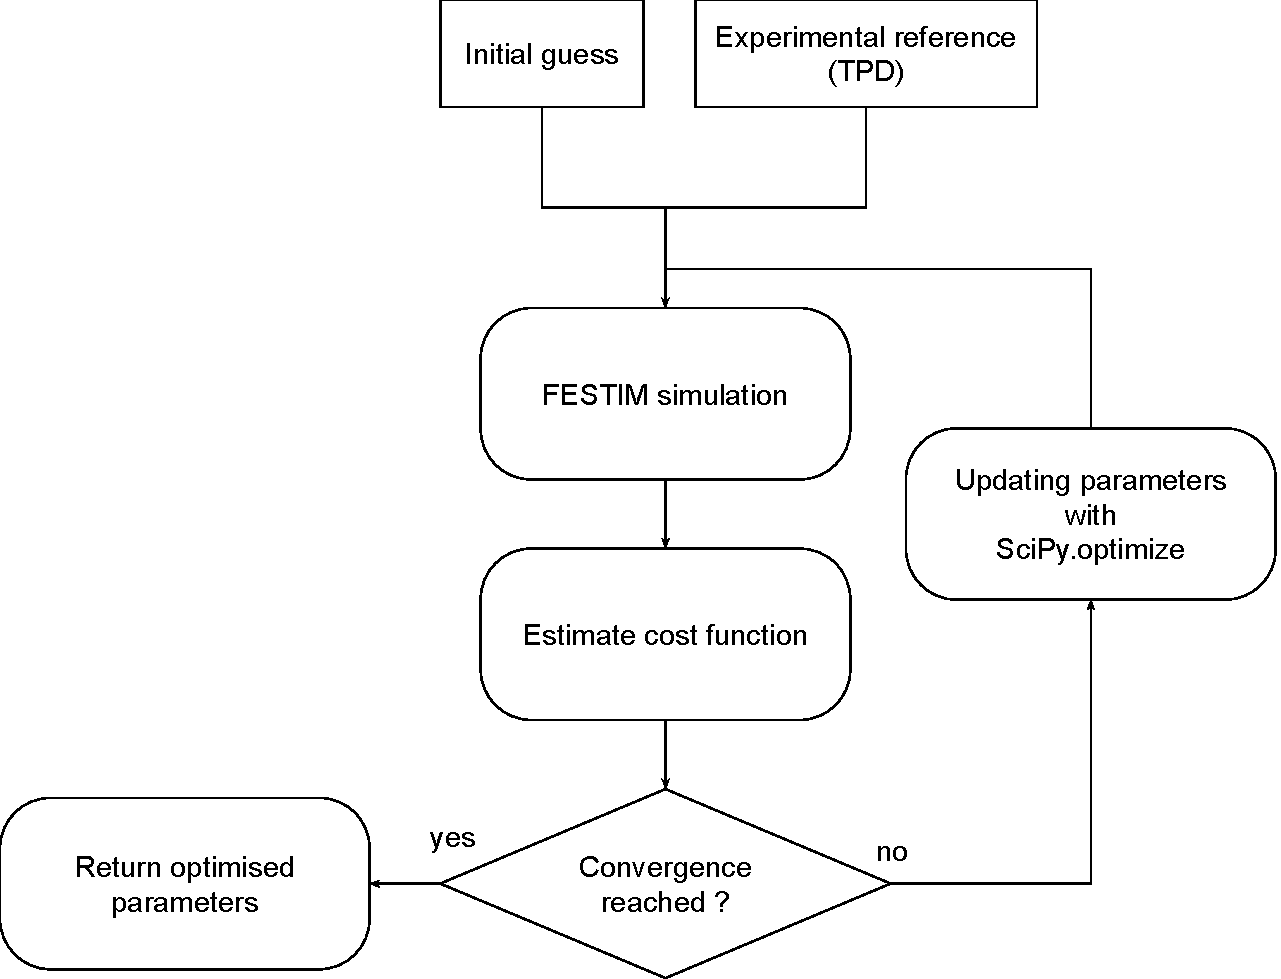
\includegraphics[width=\linewidth]{Figures/Chapter3/Parametric_optimisation/algorithm diagram.pdf}
    \caption{Diagram of the embedding of FESTIM within a parametric optimisation routine based on SciPy \cite{virtanen_scipy_2020}.}
    \label{fig:diagramm}
\end{figure}

A comparative study of the several optimisation algorithms which can be employed has been made.
These algorithms require the user to give an initial set of parameters called \textit{initial guess} and evaluate the cost function with several parameters sets until the convergence criterion is reached.
As in \sidecite{drexler_model-based_2019}, the Python package SciPy \sidecite{virtanen_scipy_2020} will be employed.

Four minimisation algorithms have been benchmarked against a test case.
In the following example an experimental \gls{tds} spectrum from Ogorodnikova et al.\ \sidecite{ogorodnikova_deuterium_2003} will be fitted and materials properties such as trap density and detrapping energy will be identified.
For this example case, two intrinsic traps and one extrinsic trap are set.
The only free parameters are $E_1$ and $n_1$, respectively the detrapping energy and density of trap 1.
The other parameters are constrained and described in \sidecite{delaporte-mathurin_finite_2019}.
The cost function $f$ has been plotted on Figure \ref{fig:cost function} as function of $E_1$ and $n_1$.

\begin{figure*} [h!]
    \centering
        \begin{subfigure}[t]{0.7\linewidth}
            \centering
            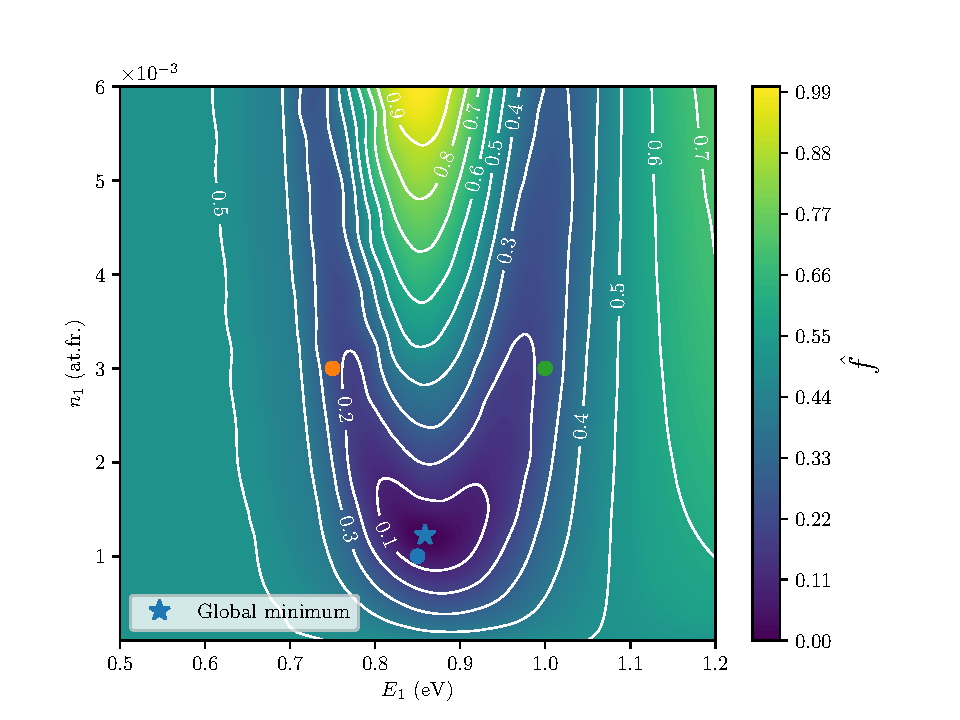
\includegraphics[width=\linewidth]{Figures/Chapter3/Parametric_optimisation/cost_function_2D.pdf}
            \caption{Normalised cost function.}
        \end{subfigure}
        \begin{subfigure}[t]{0.7\linewidth}
            \centering
            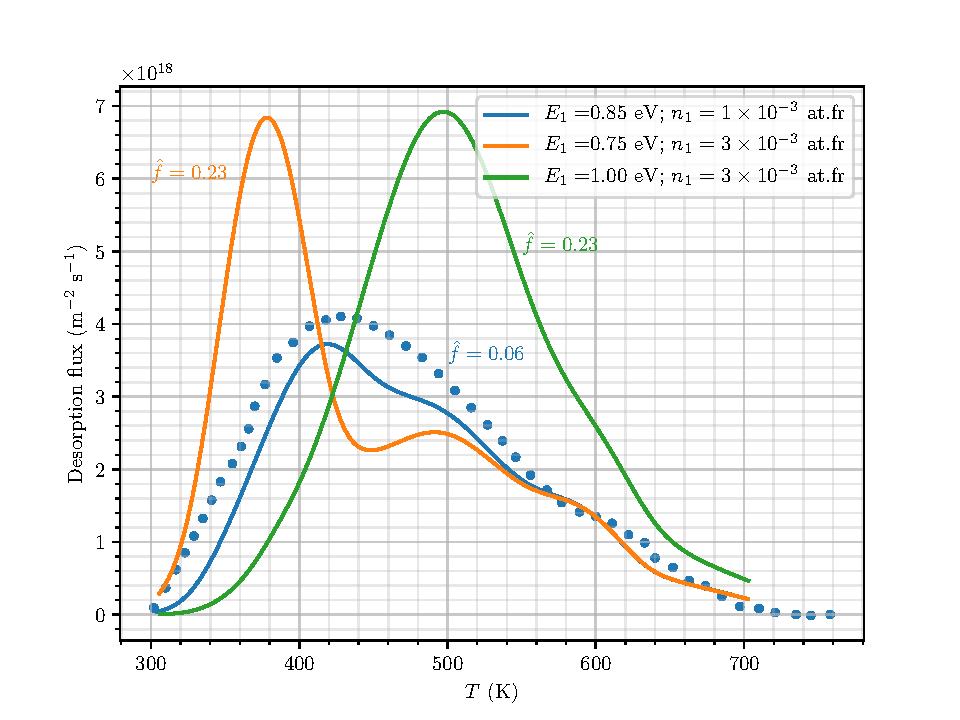
\includegraphics[width=\linewidth]{Figures/Chapter3/Parametric_optimisation/points_on_cost_function.pdf}
            \caption{Corresponding simulated \gls{tds} spectra.}
        \end{subfigure}%
    \caption{Normalised cost function $\hat{f} = (f - \min{f})/(\max{f}-\min{f})$ as function of $E_1$ (\si{eV}) and $n_1$ (\si{at.fr.}) with global minimum located at $(\SI{0.86}{eV}, \SI{1.2e-3}{at.fr.})$.}
    \label{fig:cost function}
\end{figure*}

In this case, when only two free parameters are set the cost function has only one minimum (it is not necessarily the case for higher dimension optimisation problems).
However, if one fixes the trap density $n_1$ above $\approx \SI{2e-3}{at.fr.}$, the cost function has two local minima which can lead the optimisation routine to converged to a non-global minimum.
Moreover, $f$ is smooth and quadratic around its minimum located at $(E_1, n_1) = (\SI{0.86}{eV}, \SI{1.2e-3}{at.fr.})$.
For detrapping energies below \SI{0.6}{eV} and/or densities below \SI{0.5e-3}{at.fr}, the cost function is constant.
This is because for these values, the contribution of this trapping site to the \gls{tds} spectrum is zero either because the density is close to zero, or because the energy is too low for these traps to be filled at the implantation temperature of \SI{300}{K}.
Variations in these regions do not modify the simulated spectrum and thus do not modify the cost function value.

\begin{figure} [ht]
    \centering
    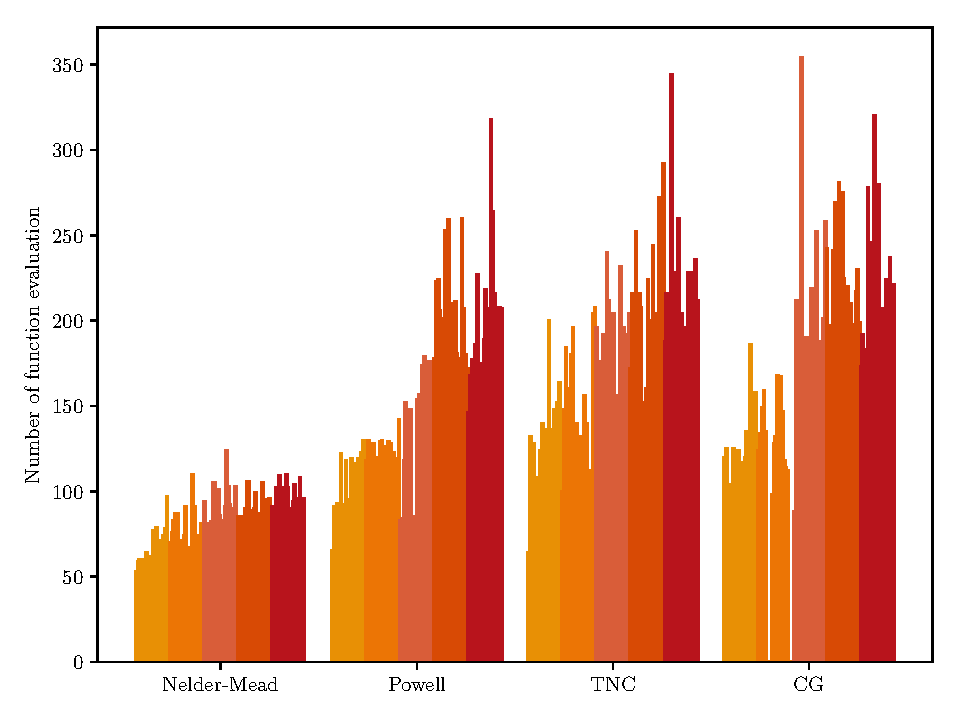
\includegraphics[width=\linewidth]{Figures/Chapter3/Parametric_optimisation/algorithms_perfs.pdf}
    \caption{Number of cost function evaluations required to converge towards the global minimum with 100 different initial guesses sorted by distance to the global minimum for several minimisation algorithms. Each cost function evaluation takes \SI{20}{s} to compute. White stripes correspond to initial guesses for which the algorithm did not converge to the global minimum.}
    \label{fig:algos perfs}
\end{figure}


Four different optimisation algorithms are being compared: 
Nelder-Mead (also called the simplex method), Powell, \gls{tnc} and \gls{cg}.
Thorough descriptions of these algorithms would be beyond the scope of this research but can be found in \sidecite{nocedal_numerical_2006}.
The performances of these algorithms have been compared with 100 different initial guesses randomly distributed on the $(E_1,n_1)$ plane and are shown on Figure \ref{fig:algos perfs}.
It appears that the \gls{cg} algorithm is less robust since for some cases it didn't converge towards the global minimum (see white bands on Figure \ref{fig:algos perfs}).
Nelder-Mead algorithm appears to be the most efficient with initial guesses both close and far from the global minimum since the number of cost function evaluations ranges from 50 to 100 whereas other algorithms require more than 100.
This can be explained by the fact that Nelder-Mead is a derivative-free algorithm whereas \gls{tnc} and \gls{cg} algorithms need on the other hand to compute first order derivatives thus increasing the number of function evaluations.
This will be even more true when increasing the number of free parameters since the derivative will become more costly to compute.

It is worth noting that the Nelder-Mead algorithm is an unconstrained method.
If constraints or bounds are needed, \gls{tnc} might be a more suitable choice.

Though in the following, the Nelder-Mead algorithm will be employed in the following cases.


% \subsubsection{Results} \label{results}

% \subsection{Applications}

% The fitting procedure has been employed to reproduce thermo-desorption experiments performed on Tungsten, EUROFER, Aluminium and Beryllium.


\subsubsection{Validation on tungsten}

The TDS spectrum measured by Ogorodnikova \textit{et al} \sidecite{ogorodnikova_deuterium_2003} has been reproduced by setting all traps parameters as free parameters.
The fitting procedure has been run for several numbers of traps as shown on Figure \ref{fig:number of traps comparison}.
It is clear that setting only one trap is not sufficient to reproduce the experimental data.
The two traps case shows better results but also has a discrepancy near \SI{600}{K}.
This discrepancy is removed when setting a third extrinsic trap to the simulation.

For this last case, the five free parameters are the detrapping energies $E_{p, 1}$, $E_{p, 2}$, $E_{p, 3}$ and densities $n_1$, $n_2$ (the third trapping site being created during the implantation, for which the creation parameters are not part of the free parameters and taken from \cite{ogorodnikova_deuterium_2003} or \sidecite{hodille_macroscopic_2015}).
This optimisation case is therefore a 5D optimisation problem.
Every other parameter is taken from \cite{hodille_macroscopic_2015}.
The resulting fit is shown on Figure \ref{fig:5D TDS} alongside with the contribution of each trap to the total spectrum.
An interesting feature of this spectrum is the negative area of the contribution of the second trap around \SI{400}{K}.
Because not all of these traps are saturated, when trap 1 is empyting, some of the hydrogen particles are nearly instantly trapped in the second trap which has a higher detrapping energy.

% (1 trap [ 0.88368005  1.44347635] 2 traps [ 0.83582125  1.23768655  0.98708714  6.85457283])
\begin{figure*} [h!]
    \centering
        \begin{subfigure}[t]{0.5\linewidth}
            \centering
            \captionsetup{width=.9\linewidth}
            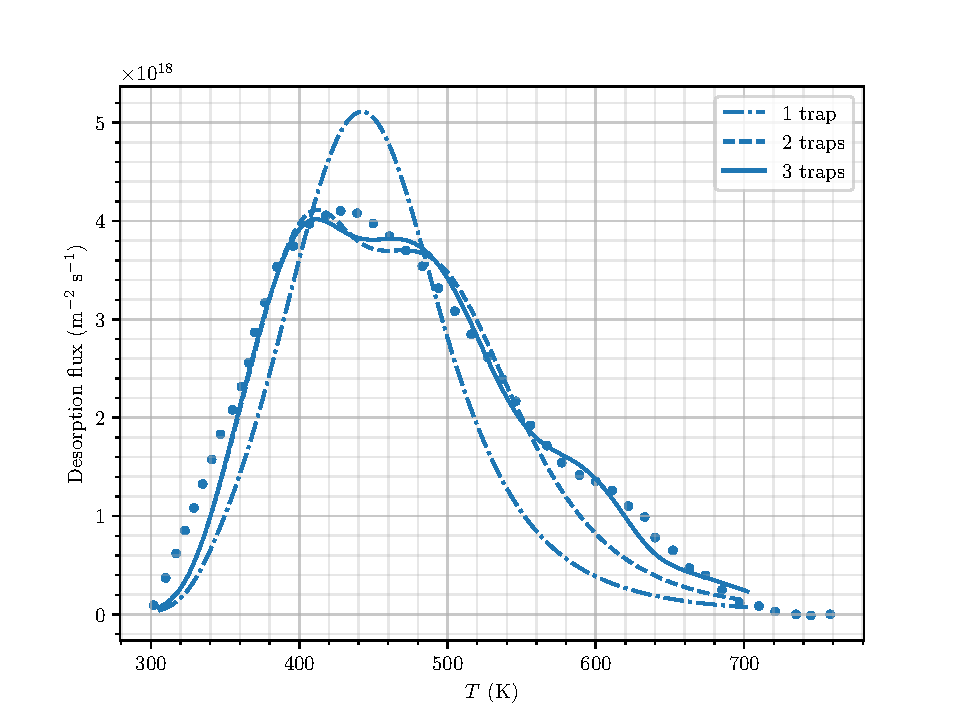
\includegraphics[width=\linewidth]{Figures/Chapter3/Parametric_optimisation/number_of_traps.pdf}
            \caption{Comparison of the resulting fit with several numbers of traps in the simulation.}
            \label{fig:number of traps comparison}
        \end{subfigure}%
        \begin{subfigure}[t]{0.5\linewidth}
            \centering
            \captionsetup{width=.9\linewidth}
            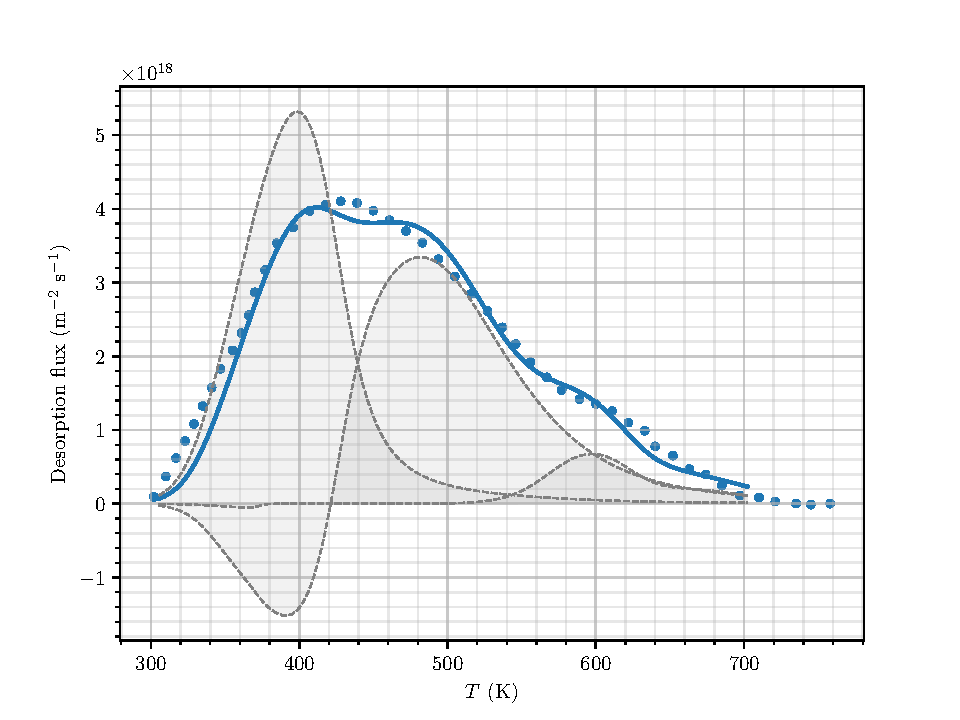
\includegraphics[width=\linewidth]{Figures/Chapter3/Parametric_optimisation/Ogorodnikova_5D.pdf}
            \caption{Identified by the fitting procedure with $E_1 = \SI{0.83}{eV}$, $E_2 = \SI{0.97}{eV}$, $E_3 = \SI{1.51}{eV}$, $n_1 = \SI{1.18e-3}{at.fr.}$ and \newline $n_2 = \SI{7.22e-4}{at.fr.}$.  Dashed lines correspond to the temporal evolution of each trapping population's inventory.}
            \label{fig:5D TDS}
        \end{subfigure}%
    \caption{Fitting TDS spectrum performed on Tungsten by Ogorodnikova \textit{et  al} \cite{ogorodnikova_deuterium_2003}. Dots correspond to experimental data.}
    \label{fig:TDS ogorodnikova}
\end{figure*}
The identified parameters are similar to the ones found by Hodille \textit{et al.} in \cite{hodille_macroscopic_2015}.
The total fitting procedure took a few hundred of cost function evaluations.
One single cost function evaluation "costing" less than \SI{20}{s} to compute (for that specific case), the total procedure lasted less than \SI{3}{h}.

% \subsubsection{EUROFER}

% Hollingsworth \textit{et al} performed thermo-desorption on pre-damaged EUROFER at several damage levels \sidecite{hollingsworth_comparative_2019}.
% Three spectra with similar exposure conditions have been fitted with one trapping site (since only one peak appears on the spectra) as shown on Figure \ref{fig:TDS EUROFER}.

% \begin{figure} [h!]
%     \centering
%     \includegraphics[width=0.9\linewidth]{Figures/Chapter3/Parametric_optimisation/EUROFER_hollingsworth.pdf}
%     \caption{TDS spectra of damaged EUROFER \cite{hollingsworth_comparative_2019}. Fitted with one trapping site (solid line) $E=\SI{1.06}{eV}$ and densities of \SI{8.9e-3}{at.fr}, \SI{2.8e-2}{at.fr} and \SI{5.0e-2}{at.fr} for \SI{0}{dpa}, \SI{0.01}{dpa} and \SI{0.1}{dpa}, respectively. Dashed lines correspond to optimisations with an unweighted cost function. Dots correspond to experimental data.}
%     \label{fig:TDS EUROFER}
% \end{figure}

% To put the emphasis on peaks, a weighting factor of 10 has been applied for $T \in [\SI{445}{K}, \SI{492}{K}]$.
% Not applying this factor near the peak region results in a closer fit in other regions but a higher peak value.
% The identified trap energy is $E_p$ \SI{1.06}{eV} for all spectra whereas the trap density $n$ is \SI{8.9e-3}{at.fr} for the undamaged sample, \SI{2.8e-2}{at.fr} for \SI{0.01}{dpa} and \newline \SI{5.0e-2}{at.fr} for \SI{0.1}{dpa}.
% For all simulations the attempt frequency $p_0$ is \SI{1e13}{s^{-1}} and the diffusion coefficient is taken from \sidecite{esteban_hydrogen_2007}.

% The total fitting procedure took less than two hours for fitting the three spectra.
% A more thorough study of these experiments could involve constraining the algorithm with profilometry data obtained by Hollingsworth \textit{et al} \cite{hollingsworth_comparative_2019}.
% Indeed, having a non-homogeneous trapping site distribution could help having a better fit of both the profilometry data and the TDS spectra. 

% \subsubsection{Aluminium}

% The experiment performed on Aluminium by Quiros \textit{et al} \sidecite{quiros_blistering_2019, quiros_blister_2017} has also been reproduced with FESTIM.

% Only one trap has been set in the simulation and its energy $E_p$ and density $n$ are set as free parameters.
% Every other parameters are fixed and taken from \cite{quiros_blister_2017, quiros_blistering_2019}.
% The resulting simulated TDS spectrum is shown on Figure \ref{fig:TDS alu}.
% \begin{figure} [h!]
%     \centering
%     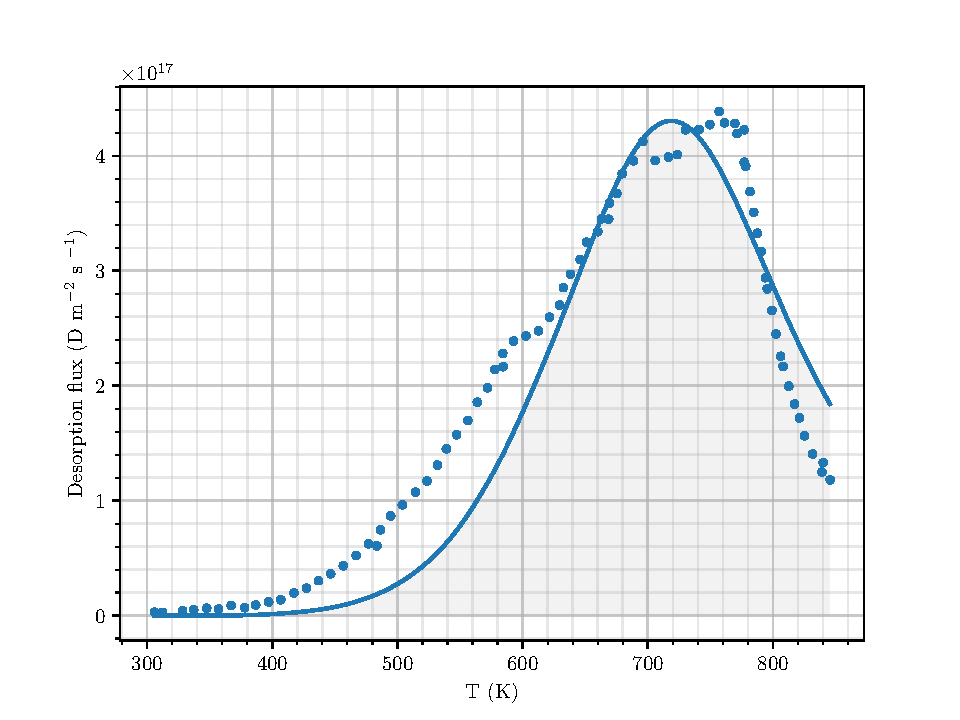
\includegraphics[width=0.9\linewidth]{Figures/Chapter3/Parametric_optimisation/alu_quiros.pdf}
%     \caption{TDS spectrum of aluminium exposed to \SI{3e23}{H.m^{-2}} at \SI{618}{K} \cite{quiros_blister_2017, quiros_blistering_2019}. Fitted with one trapping site $n = \SI{1.8e-2}{at.fr.}$ and $E =\SI{1.1}{eV}$. Dots correspond to experimental data. Dashed lines correspond to the temporal evolution of each trapping population's inventory.}
%     \label{fig:TDS alu}
% \end{figure}


% The identified parameters are $n = \SI{1.8e-2}{at.fr.}$ and $E =\SI{1.1}{eV}$.
% The trapping sites density is significantly higher than the one described in \cite{quiros_blister_2017}.
% However, the TDS spectrum obtained with this procedure better fits the experimental data since the one obtained by Quiros \textit{et al} requires a 10-fold increase.
% The fitting procedure took less than a hundred cost function evaluations, which corresponds in total to a few dozens of minutes.

% \subsubsection{Beryllium}
% Be co-deposition experiments performed by Baldwin \textit{et al} \sidecite{baldwin_experimental_2014} were reproduced.
% In this experiment, a \SI{1}{\micro m} thick Be-D layer is grown on Tungsten at \SI{330}{K}. 
% Following the strategy proposed by Baldwin \textit{et al}, only the thermo-desorption phase has been simulated with two trapping sites with homogeneously distributed densities and with initial occupancies $f_i$.
% There are therefore three free parameters per trap (energy, density and initial occupancy) which makes this optimisation problem 6D.
% It is assumed that the surface flux is the net balance between incoming flux from the chamber (very low since the pressure is $\SI{1}{\micro Pa}$) and the molecular recombination flux.
% All the other parameters are described in \cite{baldwin_experimental_2014}.

% The resulting optimised TDS spectrum is shown on Figure \ref{fig:TDS baldwin}.
% The optimised parameters are $E_{p, 1} = \SI{0.75}{eV}$, $n_1 = \SI{1.09e-1}{at.fr.}$, $f_1=0.73$, $E_{p, 2} = \SI{0.93}{eV}$, \newline ${n_2 = \SI{3.40e-2}{at.fr.}}$, $f_2=0.28$.
% These values are in agreement with the ones found by Baldwin \textit{et al} \cite{baldwin_experimental_2014} and took only a few of minutes to compute since the implantation phase was not simulated.

% \begin{figure} [h!]
%     \centering
%     \includegraphics[width=0.9\linewidth]{Figures/Chapter3/Parametric_optimisation/baldwin_be.pdf}
%     \caption{TDS spectrum of co-deposited Be-D \cite{baldwin_experimental_2014} simulated with two trapping sites. Dots correspond to experimental data.}
%     \label{fig:TDS baldwin}
% \end{figure}

\subsubsection{Limitations}

Even though an automated technique is proposed, the user still has some choices to make in order to ensure the credibility of the fitted spectrum.
As shown on Figure \ref{fig:TDS EUROFER}, weighting the cost function near regions of interest will result in a better fit in these regions.
Users should also be aware of the number of traps the data is being fitted with.
As shown on Figure \ref{fig:number of traps comparison} too few traps in the simulation will not result in a satisfactory fit (even though the optimisation routine will converge to an optimised solution).
Moreover, as shown on Figure \ref{fig:hurley_comparison}, one single TDS spectrum can be reproduced with several traps of different energies and densities.
This means that the cost function with several traps as free parameters can have several local minima of very similar values.
Adding traps to an optimisation problem can also help having a better fit of the experimental data in some cases.
But artificially adding more and more traps is not necessarily realistic and could lead to misinterpretation of the results.

\begin{figure}[h!]
    \centering
    \includegraphics[width=0.9\linewidth]{Figures/Chapter3/Parametric_optimisation/hurley_comparison.pdf}
    \caption{TDS spectrum reproduced with several sets of parameters showing the existence of several solutions to a single optimisation problem.}
    \label{fig:hurley_comparison}
\end{figure}

In the first case with only one trapping site, as described by Hurley \textit{et al} in \sidecite{hurley_numerical_2015}, the binding energy is \SI{0.55}{eV} and the trap density is \SI{2.08e24}{m^{-3}}.
The appearance of two peaks is due to the desorption on different sides of the sample as explained in \cite{hurley_numerical_2015}.
In the second case, the curve as been reproduced with two trapping sites which energies and densities are respectively \SI{0.51}{eV} and \SI{0.57}{eV} and \SI{2.02e24}{m^{-3}} and \SI{2.12e24}{m^{-3}}.
In the third case, it has been reproduced with three trapping sites which energies and densities are respectively \SI{0.55}{eV}, \SI{0.38}{eV} and \SI{0.51}{eV} and \SI{2.12e24}{m^{-3}}, \SI{2.26e24}{m^{-3}} and \newline \SI{2.13e24}{m^{-3}}.

This example illustrates how a single spectrum can be simulated with several sets of parameters by varying the number of traps in the simulation.
One way to avoid this from happening is to have a set of experiments with varying parameters such as the implantation temperature, the heating ramp, the fluence, dwelling time before TDS, etc.


\subsection{Comparison with TMAP7}

The FESTIM code was compared to TMAP7 \sidecite{longhurst_tmap7_2008} on a 1D case.

The 1D simulation case is a \SI{8.5}{mm}-thick composite slab made of W, Cu and CuCrZr (see \reffig{monoblock 1D geometry}).
The plasma facing surface $\Gamma_\mathrm{top}$ is located at $x=\SI{0}{mm}$ and the surface cooled by water $\Gamma_\mathrm{coolant}$ is located at $x=\SI{8.5}{mm}$.
The trapping parameters are detailed in \reftab{traps comparison tmap}.
The boundary conditions are detailed in \refeq{code comparison BCs}.

\begin{figure}
    \begin{overpic}[width=0.75\linewidth]{Figures/Chapter3/monoblocks/interface_condition/iter case/Monoblock 1D.pdf}
        \put(40, 50){\SI{6}{mm}}
        \put(40, 8){W}
        \put(62, 50){\SI{1}{mm}}
        \put(65, 8){Cu}
        \put(72, 50){\SI{1.5}{mm}}
        \put(72, 8){CuCrZr}
        \put(6, 25){\large$\Gamma_\mathrm{top}$}
        \put(85, 25){\large$\Gamma_\mathrm{coolant}$}
    \end{overpic}
    \caption{TMAP7 - FESTIM comparison 1D geometry showing W \cruleme[grey]{0.3cm}{0.3cm}, Cu \cruleme[orange]{0.3cm}{0.3cm}, CuCrZr \cruleme[yellow]{0.3cm}{0.3cm}.}
    \labfig{monoblock 1D geometry}
\end{figure}

\begin{table*}
    \centering
    \begin{tabular}{L{1.5cm} L{1.5cm} R{1.7cm} R{1.1cm} R{1.6cm} R{1.1cm} R{1.9cm}}
         & Material & $k_0 (\si{m^3.s^{-1}})$ &  $E_k (\si{eV})$ & $p_0 (\si{s^{-1}})$ & $E_p (\si{eV})$ & $n_i (\si{at.fr.})$ \\
        \hline
        \\
        Trap 1 & W & $3.8 \times 10^{-17}$ & 0.39 & $8.4 \times 10^{12}$& 1.20 & $5.0 \times 10^{-4}$ \\
        \\
        Trap 2 & W & $3.8 \times 10^{-17}$ & 0.39 & $8.4 \times 10^{12}$& 1.40 & $5.0 \times 10^{-3}$ \\
        \\
        Trap 3 & Cu & $6.0 \times 10^{-17}$ & 0.39 & $8.0 \times 10^{13}$ & 0.50 &$5.0 \times 10^{-5}$\\
        \\
        Trap 4 & CuCrZr & $1.2\times 10^{-16}$ & 0.42 & $8.0 \times 10^{13}$ & 0.50 &$5.0 \times 10^{-5}$\\
        \\
        Trap 5 & CuCrZr & $1.2\times 10^{-16}$ & 0.42 & $8.0 \times 10^{13}$ & 0.83 &$4.0 \times 10^{-2}$\\
        \\
    \end{tabular}
    \caption{Traps properties used in the comparison with TMAP7.}
    \labtab{traps comparison tmap}
\end{table*}

\begin{subequations}
    \begin{align}
    T &= \SI{1200}{K}\quad \text { on } \Gamma_\mathrm{top}\\
    c_\mathrm{m} &=  \frac{\varphi_\mathrm{imp} \cdot R_p}{D} \quad \text { on } \Gamma_\mathrm{top}\\
    T &= \SI{373}{K} \quad \text { on } \Gamma_\mathrm{coolant}\\
    -D \nabla c_\mathrm{m} \cdot \mathbf{n} &= K_\mathrm{CuCrZr} \cdot c_\mathrm{m}^{2} \quad \text { on } \Gamma_\mathrm{coolant}  
    \end{align}
    \labeq{code comparison BCs}
\end{subequations}
% $\varphi_\mathrm{imp} = \SI{5e23}{m^{-2}.s^{-1}}$ the implanted particle flux, $R_p = \SI{1.25}{nm}$ the implantation depth, $\mathbf{n}$ the normal vector and 
with $K_{r,\mathrm{CuCrZr}} = 2.9 \times 10^{-14}\cdot \exp{(-1.92/(k_B\cdot T))}$ the recombination coefficient of the CuCrZr (in vacuum) expressed in \si{m^4.s^{-1}} \sidecite{anderl_deuterium_1999}.

The Dirichlet boundary condition on $\Gamma_\mathrm{top}$ for the hydrogen transport corresponds to a flux balance between the implanted flux and the flux that is retro-desorbed at the surface (see \refsec{triangle model}).
The temperature profile in TMAP7 was fixed on the temperature profile produced by FESTIM (see \reffig{temperature}).

TMAP7 and FESTIM were found to be in very good agreement (see \reffig{code comparison}).

\begin{figure*} [h]
    \centering
    \includegraphics[width=0.5\linewidth]{Figures/Chapter3/monoblocks/interface_condition/iter case/temperature_1D.pdf}
    \caption{Temperature profile simulated by FESTIM for comparison case with TMAP7.}
    \labfig{temperature}
\end{figure*}

\begin{figure} [h]
    \centering
    \includegraphics[width=\linewidth]{Figures/Chapter3/monoblocks/interface_condition/iter case/comparison_codes.pdf}
    \caption{Comparison of results provided by FESTIM and TMAP7.}
    \labfig{code comparison}
\end{figure}



\section{Summary}

The macroscopic rate equations model describing the transport (diffusion and trapping) of H in solids was presented alongside with additional models such as the conservation of chemical potential at interfaces.
Due to the presence of thermally activated processes (diffusion, trapping, detrapping, surface processes...), the heat transfer equation has to be solved numerically.
All these equations are solved with the newly developed finite element code \gls{festim}, which heavily relies on \gls{fenics}.

\gls{festim} has been verified using methods such as the Method of Exact Solutions and the Method of Manufactured Solutions.
On the other hand, it was shown that \gls{festim} could be employed to reproduce experiments (TDS experiments) performed on tungsten.
This validation process could be extended by reproducing other types of experiments such as permeation experiments and profilometry.
However, this set of equation (shared amongst H transport codes) has already proven to be capable of reproducing these experiments.
This has been done, for instance, during the validation of TMAP7 \sidecite{longhurst_tmap7_2008}.

Thanks to this verification \& validation process, it was shown that (1) the hydrogen transport governing equations were correctly solved and (2) these equations can represent processes observed experimentally.

The \gls{festim} code can then be safely employed to perform analysis on tokamak components.

\setchapterimage{monoblocks2}
\setchapterpreamble[u]{\margintoc}
\chapter{Monoblocks}\label{Chapter3}\labch{Chapter3}

\section{Introduction}
ITER and DEMO divertors will be composed of small unit bricks called \textit{monoblocks} (see Figure \ref{fig: inner target photo}).
Monoblocks are typically made of a tungsten substrate with a cooling pipe running through.
This cooling channel is necessary to keep the component's temperature below its operating limit.

Several monoblock designs are currently studied for DEMO with varying dimensions, different materials for the cooling pipe or the interlayer, etc \sidecite{vizvary_european_2020, huang_tungsten_2016, hirai_use_2016, domptail_design_2020}.
The main candidate is the ITER-like design, which is the type of monoblock that will be used in ITER \cite{hirai_use_2016}.
This design has a tunsgten substrate with a CuCrZr cooling pipe and a Cu interlayer for compliance (see Figure \ref{fig: monoblocks with pipe}).
In ITER, monoblocks will be \SI{12}{mm}-thick whereas they will be thiner in DEMO (\SI{4}{mm}) \sidecite{you_european_2018}.

\begin{figure}
    \centering
    \includegraphics[width=\linewidth]{Figures/Chapter3/inner_target_iter.jpg}
    \caption{Prototype of the inner vertical target (source: ITER Organization).}
    \label{fig: inner target photo}
\end{figure}

\begin{figure}
    \centering
    \includegraphics[width=0.7\linewidth]{Figures/Chapter3/monoblocks_with_pipe.png}
    \caption{ITER-like monoblocks.}
    \label{fig: monoblocks with pipe}
\end{figure}

In order to assess the behaviour of H in the divertor, component-level simulations of monoblocks are required.

This chapter will focus on simulating H transport in ITER-like monoblocks.
First, the influence of interface conditions at the W/Cu and Cu/CuCrZr interfaces will be evaluated.
% Then, the impact of load cycling (heat and particles fluxes) will be assessed.
A parametric study will then be performed to link the monoblock H inventory to the exposure conditions.
Finally, the influence of edge effects (desorption on poloidal and toroidal gaps) will be highlighted.

\section{Interface conditions}
\begin{figure}
    \centering
    \includegraphics[width=\linewidth]{Figures/Chapter3/monoblocks/interface_condition/difference_w_wo_chemical_pot.pdf}
    \caption{Influence of continuity of chemical potential on the monoblock hydrogen inventory. The bottom plot shows the contribution of the trapped hydrogen in W, Cu and CuCrZr as well as the total mobile hydrogen for the case with continuity of chemical potential.}
    \labfig{influence of chemical potential on monoblock inventory}
\end{figure}


\begin{figure}
    \centering
    \begin{subfigure}{0.5\linewidth}
        \centering
        \includegraphics[width=\linewidth]{Figures/Chapter3/monoblocks/interface_condition/iter case/mobile_concentration.pdf}
        \caption{$c_\mathrm{m}$ (continuity of $c_\mathrm{m}$).}
    \end{subfigure}%
    \begin{subfigure}{0.5\linewidth}
        \centering
        \includegraphics[width=\linewidth]{Figures/Chapter3/monoblocks/interface_condition/iter case/mobile_chemical_pot.pdf}
        \caption{$c_\mathrm{m}$ (continuity of chemical potential).}
    \end{subfigure}
    \begin{subfigure}{0.5\linewidth}
        \centering
        \includegraphics[width=\linewidth]{Figures/Chapter3/monoblocks/interface_condition/iter case/retention_concentration.pdf}
        \caption{Retention (continuity of $c_\mathrm{m}$).}
    \end{subfigure}%
    \begin{subfigure}{0.5\linewidth}
        \centering
        \includegraphics[width=\linewidth]{Figures/Chapter3/monoblocks/interface_condition/iter case/retention_chemical_pot.pdf}
        \caption{Retention (continuity of chemical potential).}
    \end{subfigure}
    \caption{Concentration fields at $t=\SI{2e7}{s}$, $\varphi_\mathrm{heat} = \SI{7}{MW.m^{-2}}$.}
    \labfig{concentration fields w/wo chemical potential}
\end{figure}

As monoblocks are made of several materials (tungsten, copper and CuCrZr), the continuity of chemical potential across interfaces results in a mobile concentration jump (see \refsec{conservation of chemical potential}).
However, the problem could be simplified if, instead of ensuring the continuity of chemical potential, one ensured the continuity of mobile concentration across interfaces.
Indeed, this would allow getting rid of one equation and therefore reduce the computational time.
But is this simplification valid?

To verify its validity, 2D monoblock simulations are performed with chemical potential continuity (see \refeq{c/s conservation}) or mobile concentration continuity and the temporal evolution of the inventory was computed.
The implanted flux $\varphi_\mathrm{imp}$ was fixed to \SI{1.0e21}{m^{-2}.s^{-1}} and the heat flux $\varphi_\mathrm{heat}$ varied from \SI{3.0}{MW.m^{-2}} to \SI{7.0}{MW.m^{-2}}.

For the low flux cases (\SI{3}{MW.m^{-2}} and \SI{5}{MW.m^{-2}}), no difference was found (see \reffig{influence of chemical potential on monoblock inventory}).
For the case at \SI{6}{MW.m^{-2}}, differences start to appear after \SI{3e6}{s} (\SI{7e5}{s} at \SI{7}{MW.m^{-2}}).
After \SI{2e7}{s} of continuous exposure, the absolute difference at \SI{6}{MW.m^{-2}} was 25 \% and 55 \% at \SI{7}{MW.m^{-2}}.

This time of appearance of differences corresponds to the time required for the hydrogen to migrate up to the W/Cu interface.
This is explained by the high solubility ratio between W, Cu and CuCrZr leading to a higher concentration of mobile particles in CuCrZr (see \reffig{concentration fields w/wo chemical potential}) and therefore a higher trapping rate.
Since the trap density in Cu is low, the global inventory is not affected by it.


\begin{figure}
    \centering
    \begin{subfigure}{0.5\linewidth}
        \includegraphics[width=\linewidth]{Figures/Chapter3/monoblocks/interface_condition/retention_chemical_pot_short_exposure.pdf}
        \caption{continuity of chemical potential.}
    \end{subfigure}%
    \begin{subfigure}{0.5\linewidth}
        \includegraphics[width=\linewidth]{Figures/Chapter3/monoblocks/interface_condition/retention_concentration_short_exposure.pdf}
        \caption{continuity of mobile concentration.}
    \end{subfigure}
    \caption{Retention fields at $t=\SI{6.1e4}{s}$.}
    \labfig{retention fields w/wo chemical pot short exposure}
\end{figure}

Similarly, before reaching the W/Cu interface, the retention profiles are identical regardless of the interface condition (see \reffig{retention fields w/wo chemical pot short exposure}).

The retro-desorbed flux (from the monoblock to the plasma) does not depend on the interface conditions since interfaces are far from the exposed surface.
Moreover, outgassing flux through the cooling pipe greatly depends on the boundary condition imposed at the cooling surface.
Therefore, in order to assess the impact of interface conditions on the outgassing flux through the cooling pipe, uncertainties must first be lifted regarding the recombination process occurring on surfaces in contact with water.

Since this work is motivated by the estimation of the divertor inventory, the concentration continuity assumption is therefore valid since only a few monoblocks are exposed to high heat fluxes and most of the divertor is at the coolant temperature (this will be explained further in \refch{Divertor inventory estimation}).


% \section{Influence of cycling}

% \begin{itemize}
%     \item Redo one or two sims in Etienne paper ?
%     \item continuous first to load the monoblock then cycling
% \end{itemize}

\section{Exposure conditions} \label{influence of exposure conditions}

\subsection{Simulation description}
The first step of the work was to simulate the hydrogenic transport and trapping in a tungsten monoblock as a function of the loading conditions.

Moreover, a parametric study will be carried out in order to simulate the whole range of the implantation conditions encountered in the ITER divertor.

% NO NEED TO PUT THE GEOMETRY HERE AGAIN
% \subsubsection{Geometry}
% The geometry used in this work is that of a non-shaped ITER monoblock (see Figure \ref{fig:monoblock geometry}).
% The monoblocks use tungsten armour and a \SI{1.5}{mm}-thick CuCrZr pipe as heat sink.
% The pipe is jointed to the tungsten.
% A \SI{1}{mm}-thick Cu interlayer is used in order to handle stress resulting from differential thermal expansion \sidecite{richou_realization_2017}.
% The surface $\Gamma_\mathrm{top}$ is facing the plasma and $\Gamma_\mathrm{coolant}$ is cooled by water.

% \begin{figure} [ht!]
%     \centering
%     \begin{overpic}[width=\linewidth]{Figures/Chapter3/monoblocks/parametric_study/monoblock_sketch.pdf}
%         \put(42, 5){\SI{28}{mm}}
%         \put(97, 50){\SI{28}{mm}}
%         \put(10, 32){\SI{13.5}{mm}}
%         \put(42, 62){ \diameter \SI{12}{mm}}
%         \put(42, 71){ \diameter \SI{15}{mm}}
%         \put(42, 78){ \diameter \SI{17}{mm}}
%         \put(20, 80){\large$\Gamma_\mathrm{top}$}
%         \put(40, 41){\large$\Gamma_\mathrm{coolant}$}
%     \end{overpic}
%     \caption{Monoblock geometry showing W armour \cruleme[grey]{0.3cm}{0.3cm}, Cu interlayer \cruleme[orange]{0.3cm}{0.3cm}, CuCrZr alloy cooling pipe  \cruleme[yellow]{0.3cm}{0.3cm}}
%     \label{fig:monoblock geometry}
% \end{figure}

% \subsubsection{Material properties}
% The material properties used in these simulations are described in Tables \ref{tab:materials properties_2} and their temperature dependence is shown in Figure \ref{fig:properties_2}.
% The trap parameters are described in Table \ref{tab:traps monoblock}.
% Influence of mechanical fields such as thermal expansion on trap creation \sidecite{benannoune_multidimensional_2020} was not taken into account in this work.
% Hodille \textit{et al} described an extrinsic trap in tungsten created by ion implantation \sidecite{hodille_macroscopic_2015}.
% This trap is assumed to have only a small influence on the macroscopic behaviour of the monoblock and is therefore not taken into account in this work for the sake of simplicity.

% \begin{table*}[ht]
%     \centering
%     \begin{tabular}{p{1.7cm}  R{3cm}  R{3cm}  R{1.8cm}  R{2.1cm} }
%          & \multicolumn{2}{c}{Thermal properties} & \multicolumn{2}{c}{Hydrogen transport}\\
%         \hline
%         Material & $\rho \cdot C_p \newline(\si{J.K^{-1}.m^{-3}})$ & $\lambda \newline(\si{W.m^{-1}.K^{-1}})$ & $D_0 \newline(\si{m^2.s^{-1}})$ & $E_\mathrm{diff} \newline(\si{eV})$\\
%         \hline
%         \\
%         W & %
%         $5.1\times 10^{-6} \cdot T^3 \newline - 8.3\times 10^{-2}\cdot T^2 \newline + 6.0 \times 10^{2}\cdot T \newline +2.4\times 10^6$ &%
%         $-7.8\times 10^{-9}\cdot T^3 \newline %
%         +5.0\times 10^{-5}\cdot T^2 \newline%
%         -1.1\times 10^{-1} \cdot T \newline%
%         +1.8\times 10^{2}$ &%
%         $1.9\times 10^{-7}$ & 0.20 \\
%         \\
%         Cu &%
%         $1.7\times 10^{-4}\cdot T^3\newline %
%         +6.1\times 10^{-2}\cdot T^2\newline %
%         +4.7\times 10^2\cdot T\newline %
%         +3.5\times 10^6$ &%

%         $-3.9\times 10^{-8}\cdot T^3\newline %
%         +3.8\times 10^{-5}\cdot T^2\newline %
%         -7.9\times 10^{-2}\cdot T\newline %
%         +4.0\times 10^2 $&%

%         $6.6\times 10^{-7}$ &%
%         0.39\\
%         \\
%         CuCrZr & %
%         $-1.8\times 10^{-4}\cdot T^3 \newline %
%         +1.5\times 10^{-1}\cdot T^2\newline %
%         +6.2\times 10^2\cdot T\newline %
%         +3.5\times 10^6$ &%

%         $5.3\times 10^{-7}\cdot T^3\newline %
%         -6.5\times 10^{-4}\cdot T^2\newline %
%         +2.6\times 10^{-1}\cdot T\newline %
%         +3.1\times 10^2$ & %

%         $3.9\times 10^{-7}$ & %
%         0.42\\
%         \\
%     \end{tabular}
%     \caption{Materials properties used in the simulations. Thermal properties are fitted from ANSYS. \cite{reiter_compilation_1996, serra_hydrogen_1998, fernandez_hydrogen_2015}}
%     \label{tab:materials properties_2}
% \end{table*}

% \begin{figure*} [h!]
%     \centering
%     \begin{subfigure}{0.5\linewidth}
%         \centering
%         \includegraphics[width=\linewidth]{Figures/Chapter3/monoblocks/parametric_study/thermal_prop.pdf}
%     \end{subfigure}%
%     \begin{subfigure}{0.5\linewidth}
%         \centering
%         \includegraphics[width=\linewidth]{Figures/Chapter3/monoblocks/parametric_study/D_coeff.pdf}
%     \end{subfigure}
%     \caption{Material properties used in the simulations \cite{reiter_compilation_1996, serra_hydrogen_1998, fernandez_hydrogen_2015}}
%     \label{fig:properties_2}
% \end{figure*}

% \begin{table*} [ht]
%     \centering
%     \begin{tabular}{L{1.5cm} L{1.5cm} R{1.6cm} R{1.1cm} R{1.6cm} R{1.1cm} R{2cm}}
%          & Material & $k_0 (\si{m^3.s^{-1}})$ &  $E_k (\si{eV})$ & $p_0 (\si{s^{-1}})$ & $E_p (\si{eV})$ & $n_i (\si{at.fr.})$ \\
%         \hline
%         \\
%        Trap 1 & W & $3.1 \times 10^{-16}$ & 0.20 & $8.4 \times 10^{12}$& 1.00 & $1.1 \times 10^{-3}$ \\
%         \\
%         Trap 2 & Cu & $6.0 \times 10^{-17}$ & \textcolor{black}{0.39} & $8.0 \times 10^{13}$ & 0.50 &$5.0 \times 10^{-5}$\\
%         \\
%         Trap 3 & CuCrZr & $1.2 \times 10^{-16}$ & \textcolor{black}{0.42} & $8.0 \times 10^{13}$ & 0.85 &$5.0 \times 10^{-5}$\\
%         \\
%     \end{tabular}
%     \caption{Traps properties used in the simulations \cite{hodille_macroscopic_2015, dolan_assessment_1994}}
%     \label{tab:traps monoblock}
% \end{table*}

\subsubsection{Boundary conditions}

Mobile particles concentration $c_\mathrm{m}$ is imposed on $\Gamma_\mathrm{top}$ which allows to simulate particle implantation without having to include a volumetric source term applied on the first few nanometres.
This approximation allows to have a broader mesh and therefore saves computation time without affecting the macroscopic behaviour.
Molecular recombination is assumed on $\Gamma_\mathrm{coolant}$.
Even though it could be assumed on the gaps between monoblocks, it can be shown that its influence on the macroscopic behaviour remains low.
Desorption from the other surfaces is therefore assumed to be zero for simplification purposes.
\textcolor{black}{Uniform} heat loads $\varphi_H$ are applied on the surface $\Gamma_\mathrm{top}$ with a Neumman boundary condition or temperature is constrained on $\Gamma_\mathrm{top}$ with a Dirichlet boundary condition and a convective exchange condition is set on surface $\Gamma_\mathrm{coolant}$.
All the other surfaces are assumed thermally insulated.
The set of boundary conditions can finally be described as follow:

\begin{subequations}
    \begin{align}
    -\lambda \vec{\nabla} T \cdot \vec{n} &=\varphi_{H} \quad \text{or} \quad T = T_\mathrm{surface}\quad &\text { on } \Gamma_\mathrm{top}\\
    c_\mathrm{m} &=  c_\mathrm{surface}\quad &\text { on } \Gamma_\mathrm{top}\\
    -\lambda \vec{\nabla} T\cdot \vec{n} &= -h \cdot \left(T_\mathrm{coolant} - T\right)\quad &\text { on } \Gamma_\mathrm{coolant}\\
    -D \vec{\nabla} c_\mathrm{m} \cdot \vec{n} &= K_\mathrm{CuCrZr} \cdot c_\mathrm{m}^{2} \quad &\text { on } \Gamma_\mathrm{coolant}
    \end{align}
\end{subequations}
with $h=\SI{70000}{W.m^{-2}.K^{-1}}$ being the heat exchange coefficient calculated from the Sieder-Tate correlation for the forced convection regime, $T_\mathrm{coolant}= \SI{323}{K}$ and $\vec{n}$ the normal vector and $K_\mathrm{CuCrZr} = 2.9 \times 10^{-14}\cdot \exp{(-1.92/(k_B\cdot T))}$ the recombination coefficient of the copper alloy (in vacuum) expressed in \si{m^4.s^{-1}} \sidecite{anderl_deuterium_1999}.

% The thermal response of ITER-like monoblocks to the heat load $\varphi_H$ has first been studied.
% Then the hydrogen inventory was determined as a function of surface temperature and surface concentration and as a function of the implanted particle flux and the incident ion energy.
% Finally, an application on ITER exposure conditions was made.

\subsection{Thermal behaviour}
Steady-state heat transfer simulations were performed with FESTIM with varying heat loads $\varphi_H$.
With $\varphi_H = \SI{1}{MW.m^{-2}}$, the surface temperature of the monoblock was found to be around \SI{400}{K} (see Figure \ref{fig:T field 1 MW}) whereas with $\varphi_H = \SI{10}{MW.m^{-2}}$ the surface was around \SI{1400}{K} (see Figure \ref{fig:T field 10 MW}).

\begin{figure*} [h!]
    \centering
    \begin{subfigure}{0.4\linewidth}
        \centering
        \includegraphics[width=\linewidth]{Figures/Chapter3/monoblocks/parametric_study/T_1e6.pdf}
        \caption{Temperature field with $\varphi_H = \SI{1}{MW.m^{-2}}$}
        \label{fig:T field 1 MW}
    \end{subfigure}%
    \begin{subfigure}{0.4\linewidth}
        \centering
        \includegraphics[width=\linewidth]{Figures/Chapter3/monoblocks/parametric_study/T_1e7.pdf}
        \caption{Temperature field with $\varphi_H = \SI{10}{MW.m^{-2}}$}
        \label{fig:T field 10 MW}
    \end{subfigure}
    \begin{subfigure}{0.7\linewidth}
        \centering
        \includegraphics[width=\linewidth]{Figures/Chapter3/monoblocks/parametric_study/temperature_phi_H.pdf}
        \caption{\textcolor{black}{Evolution of surface temperature as a function of heat flux}}
        \label{fig:T phi_H}
    \end{subfigure}
    \caption{Thermal behaviour of the monoblock}
\end{figure*}

$T_\mathrm{surface}$ \textcolor{black}{therefore} increases linearly with the heat load and can be modelled by Equation \ref{eq:thermal behaviour law} (see Figure \ref{fig:T phi_H}).
\begin{equation}
    T_\mathrm{surface} = 1.1 \times 10^{-4} \cdot \varphi_H + T_\mathrm{coolant}
    \label{eq:thermal behaviour law}
\end{equation}

This was found to be in very good agreement with experimental measurements performed in \sidecite{hirai_use_2016}.

\subsection{Influence of \texorpdfstring{$T_\mathrm{surface}$}{Tsurface} and \texorpdfstring{$c_\mathrm{surface}$}{csurface} on hydrogen inventory}

In this section, the total inventory of hydrogen in monoblocks has been calculated as a function of $T_\mathrm{surface}$ and $c_\mathrm{surface}$.
Temperature and mobile concentration of hydrogen were imposed with Dirichlet boundary conditions on $\Gamma_\mathrm{top}$ with $T_\mathrm{surface}$ varying from $T_\mathrm{coolant}$ to \SI{1200}{K} and $c_\mathrm{surface}$ varying \textcolor{black}{arbitrarily} from \SI{e20}{m^{-3}} to \SI{6e22}{m^{-3}}.
The assumption of a constant surface temperature had low influence on the results compared to a non-homogeneous surface temperature that could be obtained with a heat flux condition since surface temperature gradient was low compared to the one between the top surface and the cooling surface.
For surface temperatures below \SI{500}{K}, 1D simulations were performed for the penetration depth of hydrogen remained very low (a few microns) and 1D approximation was sufficient \sidecite{benannoune_numerical_2019}.
For temperatures above \SI{500}{K} for which edge effects become dominant, 2D simulations have been performed.

After $ \SI{e7}{s}$ a high retention zone appeared far from the exposed surface $\Gamma_\mathrm{top}$ (see Figure \ref{fig:retention fields}).
As described in \sidecite{delaporte-mathurin_finite_2019}, this is due to thermal effects.
As seen in Figures \ref{fig:T field 1 MW} and \ref{fig:T field 10 MW}, the temperature was found to decrease in regions close to the cooling pipe $\Gamma_\mathrm{coolant}$ leading to an increase in trap occupancy, creating this high retention zone.
This was however not true for monoblocks where $T_\mathrm{surface} \approx T_\mathrm{coolant}$ since the temperature gradient in the domain is very low.
Instead, trap occupancy was close to one and the retention was high in the whole region where hydrogen had penetrated and not only far from the top surface.

\begin{figure*}
    \centering
    \begin{subfigure}{0.5\linewidth}
        \centering
        \includegraphics[height=\linewidth]{Figures/Chapter3/monoblocks/parametric_study/retention_T=7.000e+02;c=1.00e+20.pdf}
        \caption{$T_\mathrm{surface} = \SI{700}{K}$ and $c_\mathrm{surface} = \SI{e20}{m^{-3}}$}
    \end{subfigure}%
    \begin{subfigure}{0.5\linewidth}
        \centering
        \includegraphics[height=\linewidth]{Figures/Chapter3/monoblocks/parametric_study/retention_T=1.000e+03;c=1.00e+21.pdf}
        \caption{$T_\mathrm{surface} = \SI{1000}{K}$ and $c_\mathrm{surface} = \SI{e21}{m^{-3}}$}
    \end{subfigure}
    \caption{Retention fields in \si{m^{-3}} after a \SI{e7}{s} exposure}
    \label{fig:retention fields}
\end{figure*}


Hydrogen inventory in monoblocks as a function of $T_\mathrm{surface}$ and $c_\mathrm{surface}$ is shown in Figure \ref{fig:inventory T c}.
In order to obtain this continuous field, more than 600 simulations randomly distributed on the parameter plane were run and analysed using a Gaussian process machine learning algorithm \sidecite{rasmussen_gaussian_2006} as in \sidecite{shimwell_multiphysics_2019} based on the python package inference-tools \sidecite{chris_bowman_c-bowmaninference-tools_2020}.
In Figure \ref{fig:inventory T c}, the inventory obtained by the Gaussian regression process is given for a constant value of $c_\mathrm{surf}=\SI{2e21}{m^{-3}}$ (top inset) and a constant temperature $T=\SI{850}{K}$ (left inset).
The Gaussian regression process was particularly appropriate as it calculates a confidence interval based on the standard deviation $\sigma$.
As expected, the lower the density of simulation points, the higher was the value of $\sigma$ (for example around \SI{850}{K} on the top inset of Figure \ref{fig:inventory T c}).
However, despite the lack of simulation in this region, the value of $\sigma$ was still acceptable (only a few percents of the inventory) ensuring the quality of the resulting interpolation.

As expected, inventory was found to globally increase with $c_\mathrm{surface}$.
For $T_\mathrm{surface} > \SI{550}{K}$, the inventory tended to decrease with surface temperature.
However, for $T_\mathrm{surface} < \SI{550}{K}$, inventory increased with surface temperature.
This phenomenon is due to a trade-off between an increase of the detrapping rate and an increase of the diffusion coefficient making the hydrogen particles penetrate deeper into the bulk.
Above $\SI{550}{K}$, detrapping becomes dominant and inventory decreases.
This mapping of inventory as a function of $T_\mathrm{surface}$ and $c_\mathrm{surface}$ provides an easy way of estimating the inventory in monoblocks for several exposure conditions without having to run many simulations.
Indeed, to estimate the inventory with different exposure conditions, one only needs to associate these conditions $(\varphi_\mathrm{inc}, E)$ to a couple $(c_\mathrm{surf}, T_\mathrm{surf})$.

\begin{figure*} [h]
    \centering
    \includegraphics[width=\linewidth]{Figures/Chapter3/monoblocks/parametric_study/inventory_T_c_profiles.pdf}
    \caption{Evolution of the inventory after a \SI{e7}{s} exposure as a function of $T_\mathrm{surface}$ and $c_\mathrm{surface}$ alongside with simulation points (grey crosses). The simulations points were fitted with a Gaussian regression process \cite{chris_bowman_c-bowmaninference-tools_2020} providing the standard deviation $\sigma$.}
    \label{fig:inventory T c}
\end{figure*}

\subsection{Discussion}
If this methodology provides a rapid way of estimating hydrogen content in the whole divertor, several assumptions have however been made.


% Influence of cycling
First, a steady state exposure was considered for simplification purposes.
This result is however conservative.
As seen in \sidecite{delaporte-mathurin_finite_2019, hodille_estimation_2017}, cycling effects could have an influence in regions where $T_\mathrm{surface}$ varies a lot, for example \textcolor{black}{within \SI{10}{cm} on both sides of the strike points}.
Though, since a large majority of monoblocks stay at room temperature, even during operations the thermal effect should remain low and discrepancies would rather be due to particle flux evolution along the target.

% shaping
Shaping of monoblocks (\textit{e.g.} chamfers) was not taken into account in this work for simplification purposes.
Such shaping can have an influence on the incident particle and heat loads on the plasma facing surface of the monoblocks.



% Be deposits
This study presents the hydrogen trapping in W monoblocks.
It shows that the latter remains low but, as already pointed out by JET studies, the trapping on Be co-deposited layers is expected to be the main mechanism for tritium retention in ITER \sidecite{brezinsek_beryllium_2015, heinola_fuel_2015}.
Such layers could be found in the cold regions of the divertor but as soon as the strike points hit these layers, they should be sputtered away (as sputtering of Be is possible even at low energy \sidecite{bjorkas_variables_2013} \cite{brezinsek_beryllium_2015}).
The retention where the deposited layers are not present (either sputtered or not formed anyway) would then be given by the model presented here.

% Coolant recombination
The molecular recombination coefficient at the surface of the cooling pipe was taken from \sidecite{anderl_deuterium_1999} and was measured in vacuum.
One could argue that recombination in presence of water will be facilitated.
It can however be shown that this parameter has very low influence on the inventory since it was dominated by retention in tungsten.
This parameter will however have an influence on the permeation flux and should be studied in future work.

% Gap recombination
\textcolor{black}{Similarly, the influence on molecular recombination on the sides of the monoblock was found to have a low impact on the results.
By assuming an instantaneous recombination coefficient, the relative error on the monoblock inventory was found to be significant only in hot regions (\textit{ie} within \SI{10}{cm} on both sides of the strike points).
The influence on the total divertor inventory is therefore low (less than \SI{5}{\%} after a \SI{e7}{s} exposure) since it is dominated by regions where $T_\mathrm{surface} \approx T_\mathrm{coolant}$.}

% ELMs
It should be noted that specific scenarii like edge localised modes (ELMs) were also not taken into account in this work since their time scale is very short.
MRE simulations by Hu and Hassanein \sidecite{hu_predicting_2015} suggest that a \SI{400}{s} discharge with \SI{1}{Hz} or \SI{10}{Hz} ELMs significantly reduces (77 \%) the inventory in W materials.
However, the modelling of the ELM is simulated by increasing the temperature for a very short time without changing the incident flux of particles that can also be much higher thus balancing the fuel retention reduction.
Another study by Schmid \textit{et al} \sidecite{schmid_diffusion-trapping_2016} also simulated the effect of \SI{1}{Hz} ELMs on fuel retention in W.
The outcome is that \SI{6}{s} of \SI{1}{Hz}-ELMs does not affect significantly the fuel retention, though the temperature excursion in those simulations are smaller than for the one of Hu and Hassanein.
Thus, the effect of ELMs, especially the balance between increase of heat flux, incident energy and particle flux, could either favour or disfavour trapping, diffusion and migration and therefore the overall retention.

% Surface process
In this study the model to link the concentration of mobile particles at the surface (implantation zone) with the exposure condition considers that the particles are implanted in the bulk and that the recombination coefficient is very high since many uncertainties concerning the recombination coefficient are yet to be lifted.
However, if an exothermic process is considered as in \sidecite{ogorodnikova_recombination_2019}, this should have low influence since recombination is very quick at a temperature close to that of the coolant.

On the other hand, experimental results \sidecite{t_hoen_strongly_2013} suggest that for ion energy below \SI{5}{eV/H}, typical of detached plasma as the one treated in the previous section, the surface process can be important and limits the uptake of hydrogen, i.e. the adsorption on the surface and the further absorption from surface to bulk could be the limiting process for the growth of $c_\mathrm{surface}$ during such exposure.
The evolution of $c_\mathrm{surface}$ to the exposure condition for that range of energy would therefore be different and therefore the inventory.
The advantage of the presented method is that taking into account such process is realtively easy as no expensive simulations are needed.
One would only need to modify the model giving $c_\mathrm{surface}$
as a function of $(E_\mathrm{inc},\varphi_\mathrm{inc})$ to include the different surface processes.
To this end, one can use kinetic surface models \sidecite{hodille_retention_2017, zaloznik_deuterium_2017, pecovnik_influence_2019, guterl_effects_2019}.

% traps
Trap properties have a great impact on the inventory.
In this study, a homogeneous trap distribution is assumed for simplification purposes.
A more thorough study could investigate the influence on trap distribution, energy and density.
Trap properties might also vary along the divertor based on exposure conditions.
Moreover the impact of neutrons must be assessed as neutron-induced traps have a high detrapping energy.


% Helium

Finally, helium implantation in the materials and bubble formation could modify the hydrogen transport in monoblocks.

\subsection{Summary}
ITER-like monoblocks have been studied using a novel method in order to estimate the hydrogen content as a function of exposure conditions such as the implanted particle flux, the ion energy, the heat load and the monoblock surface temperature.
Several hundred data points have been simulated with FESTIM and analysed to estimate the hydrogen inventory in monoblocks for any input conditions using a Gaussian regression process, a machine learning algorithm which calculates the confidence interval for each point.
Thanks to this relation, one can easily estimate hydrogen content in the whole divertor without having to run all the simulations.
An application has been made based on the output from a SOLPS calculation of exposure conditions distribution on the ITER divertor and shows that for these conditions the inventory could reach \SI{e20}{H} per monoblock near strike points after a \SI{e7}{s} exposure.
The total hydrogen content in ITER divertor is estimated to be \SI{8}{g} which is well below the inner-vessel safety limit of \SI{1}{kg}.

This behaviour law will be used in \refch{Divertor inventory estimation} to estimate the hydrogen inventory of WEST and ITER divertors.

\section{Edge effects} \label{3D edge effects}
\subsection{Methodology}
\subsection{Standard case}

\begin{figure}
    \centering
    \includegraphics[width=\linewidth]{Figures/Chapter3/monoblocks/3D_monoblocks/inventory.pdf}
    \caption{Temporal evolution of the monoblock inventory.}
\end{figure}


\begin{figure}
    \centering
    \includegraphics[width=\linewidth]{Figures/Chapter3/monoblocks/3D_monoblocks/fluxes.pdf}
    \caption{Temporal evolution of outgassing fluxes.}
\end{figure}

\subsection{Influence of the monoblock thickness}

\begin{figure}
    \centering
    \includegraphics[width=\linewidth]{Figures/Chapter3/monoblocks/3D_monoblocks/influence_of_thickness.pdf}
    \caption{Temporal evolution of the ratio $\mathrm{inv}_\mathrm{desorption} / \mathrm{inv}_\mathrm{no desorption}$ for several thicknesses.}
\end{figure}

\subsection{Summary}

\section{Summary}
H transport in ITER-like monoblocks was simulated with FESTIM.
Several aspects of the simulations were studied.

It was shown that the choice of interface conditions (continuity of chemical potential or continuity of mobile concentration) had low impact on the monoblock inventory.
Depending on the boundary condition used at the cooling surface of the monoblock, it could however have an impact on the permeation flux.

The effect of loading cycles was also investigated.
Between plasma pulses, a zone with higher retention appears near the plasma exposed surface due to the temperature variation.
These modifications of the retention fields vanish as soon as the next cycle starts again and this zone is heated up again.
This means that cycling has no effect on the global retention field and that cycles can safely be concatenated (continuous exposure) to simulate H transport.

A parametric study was then performed in order to assess the influence of exposure conditions (surface concentration and surface temperature).
A 2D behaviour law was obtained correlating exposure conditions to the monoblock inventory.
This law will be extremely useful to estimate H retention in divertors since not all monoblocks will be exposed to the same exposure.

Finally, 3D simulations of DEMO ITER-like monoblocks have been run.
The desorption on the poloidal and toroidal gaps drastically reduced the inventory while increasing the outgassing flux to the vacuum chamber.
The permeation flux to the coolant decreased.
This means that 2D simulations are conservative in terms of H inventory.
This however undersestimates outgassing fluxes.
Future work should involve refining the behaviour law obtained in Section \ref{influence of exposure conditions} by running new 3D simulations and compute not only the H inventory but also the total outgassing.

\setchapterimage{west_div_roux_cropped}
\setchapterpreamble[u]{\margintoc}
\chapter{Divertor inventory estimation}\label{Chapter4}\labch{Chapter4}
\labch{Divertor inventory estimation}
\section{Introduction}
Hydrogen isotopes (H\footnote{H will be used to refer to all isotopes and mainly tritium}) transport in tokamaks is a crucial issue for several reasons.
First, for safety reasons, the total inventory of radioactive material trapped in the reactor must be limited to a certain amount.
In ITER, the limit of tritium in the vacuum vessel is \SI{1}{kg} \sidecite{temmerman_influence_2018}.
Second, outgassing of hydrogen from the monoblocks composing the divertor and from the tokamak first wall can reduce the plasma performances \sidecite{grisolia_plasma_1999}.
Finally, the lifespan of plasma facing components can be reduced due to hydrogen-induced damage (including embrittlement \sidecite{dwivedi_hydrogen_2018}).

Numerical modelling of H transport and retention in and outgassing from plasma facing components \sidecite{delaporte-mathurin_parametric_2020, delaporte-mathurin_influence_2021, denis_dynamic_2019, dark_influence_2021} is therefore often required in order to tackle both issues. 
These simulations are supported by experimental work to determine key properties of fusion materials.
H transport in monoblocks has been studied in 1D \sidecite{hodille_estimation_2017}.
However, it was shown in \sidecite{delaporte-mathurin_finite_2019} that the 2D edge effects had to be considered to have a better estimate of the H retention in the actively cooled divertor monoblocks.
A recent major effort has been made to perform multi-dimensional simulations \cite{delaporte-mathurin_finite_2019, delaporte-mathurin_parametric_2020, delaporte-mathurin_influence_2021, benannoune_multidimensional_2020}.

In a previous study \cite{delaporte-mathurin_parametric_2020}, the finite element code FESTIM \sidecite{delaporte-mathurin_finite_2019, delaporte-mathurin_influence_2021} was employed to simulate H isotopes transport in ITER-like monoblocks with the geometry given in \sidecite{richou_realization_2017} coupled to heat transfer.
A novel method was developed to rapidly estimate the H inventory in the whole ITER divertor from plasma code results without having to run additional finite element simulation. Instead, a behaviour law relying on a data base of 600 FESTIM simulations correlates the H inventory in a monoblock to its surface temperature and surface concentrations (using a gaussian regression process as described in \sidecite{chris_bowman_c-bowmaninference-tools_2020}).

The current work applies this technique to estimate the H inventory in the divertors of WEST and ITER based on SolEdge3X-EIRENE \sidecite{bufferand_three-dimensional_2019} and SOLPS-ITER \sidecite{kaveeva_solps-iter_2020} plasma simulations, respectively.
The influence of control parameters such as the input power, the puffing rate and the divertor neutral pressure is investigated.


\section{Methodology}
\begin{figure}[h!]
    \centering
    \includegraphics[width=0.95\linewidth]{Figures/divertor/coordinates.pdf}
    \caption{Geometry of WEST and ITER divertors}
    \label{fig: reactors}
\end{figure}

The H inventory of the WEST and ITER divertors will be computed by making use of a database of FESTIM simulations of H transport in ITER-like monoblocks from which a behaviour law is extracted using a gaussian regression process from the inference-tools python package \sidecite{chris_bowman_c-bowmaninference-tools_2020}.
These simulations model H transport in monoblocks for a fixed plasma exposure duration of \SI{e7}{s}.
This corresponds to approximately 25 000 concatenated ITER discharges of \SI{400}{s} each.
As shown in \sidecite{hodille_modelling_2021}, this approximation does not affect the H inventory in monoblocks with the current conditions.

These results are then interfaced with the exposure conditions obtained with the plasma simulations performed with the codes SOLPS \sidecite{kaveeva_solps-iter_2020} and SOLEDGE \sidecite{bufferand_three-dimensional_2019}.


\begin{figure*}[h]
    \centering
    \begin{subfigure}{0.5\linewidth}
        \includegraphics[width=\linewidth]{Figures/divertor/implantation_range.pdf}
        \caption{Implantation range $R_p$}
        \label{fig: implantation range vs energy}
    \end{subfigure}%
    \begin{subfigure}{0.5\linewidth}                          
        \includegraphics[width=\linewidth]{Figures/divertor/reflection_coeff.pdf}
        \caption{Reflection coefficient $r$}
        \label{fig: reflection coeff vs energy}
    \end{subfigure}
    \caption{Evolution of the implantation range and the reflection coefficient as a function of incident energy $E$ and angle of incidence.}
\end{figure*}

\subsection{Plasma simulations}
In this Section, the set-ups for the computation of the plasma exposure parameters are described.
For the SolEdge3X-EIRENE runs, the puff rate and the input power were used as control parameters.
For SOLPS-ITER calculation, the divertor neutral pressure is the control parameter.
\subsubsection{SolEdge3X-EIRENE runs}
The Lower-Single-Null magnetic configuration used for the 2D simulations in SolEdge3X-EIRENE transport code (v588.165) are based on the experimental WEST plasma discharge \#54903 at $T_\mathrm{flat-top} = \SI{8}{s}$ (see Figure \ref{fig: reactors}).
In order to get as many divertor conditions as possible, the puff rate was varied from \SI{4.5e20}{molecule.s^{-1}} to \SI{4.72e21}{molecule.s^{-1}} and the input power from \SI{0.449}{MW} to \SI{2.5}{MW}.
The setup parameters of the simulation are listed in Table \ref{tab: my_tab}.
$R_\mathrm{wall}$ is the recycling coefficient of main chamber wall, $R_\mathrm{pump}$ is the recycling coefficient of the pump, $D_\mathrm{m}$ is the cross-field mass diffusivity perpendicular to the flux surface, $\nu$ is the momentum diffusivity, $\chi_e$ and $\chi_i$ are the heat flux diffusivity for electrons and ions, respectively.
The gas puff position is set inside the private region and the pump position is set under the baffle.

\begin{table}[!ht]
    \centering
    \caption{Setup parameters used in the SOLEDGE3X simulations}
    \begin{tabular}{L{0.4\linewidth}  R{0.4\linewidth}}
    \hline \\
    Plasma composition & Deuterium, no impurity \\
    \\
    Recycling coefficients &  $R_\mathrm{wall} = 0.99$ \\
     & $R_\mathrm{pump} = 0.95$ \\
    \\
    SOL input power & from \SI{0.449}{MW} to \SI{2.5}{MW} \\
    \\
    Gas puff rate & from \SI{4.5e20}{molecule.s^{-1}} to \SI{4.72e21}{molecule.s^{-1}} \\
    \\
    Drifts & - \\
    \\
    Transport coefficients & $D_\mathrm{m} = \SI{0.3}{m^2.s^{-1}}$ \\
     & $\nu = \SI{0.3}{m^2.s^{-1}}$ \\
     & $\chi_e = \chi_i = \SI{1.0}{m^2.s^{-1}}$ \\
    \end{tabular}
    \label{tab: my_tab}
\end{table}


\subsubsection{SOLPS runs}
Several ITER cases were taken with divertor neutral pressures varying from \SI{1.8}{Pa} to \SI{11.2}{Pa}.
These SOLPS \sidecite{kaveeva_solps-iter_2020} scenarios can be found in the ITER Integrated Modelling Analysis Suite (IMAS) database \sidecite{imbeaux_design_2015, park_assessment_2020}.
The nine simulations used in this work are labelled 122396, 122397, 122398, 122399, 122400, 122401, 122402, 122403 and 122404.
These have been run in baseline burning plasma conditions (Q=10) and with an averaged separatrix Ne concentration of around \SI{0.6}{\%} \sidecite{pitts_physics_2019}.


\begin{figure}[h!]
    \centering
    \includegraphics[width=\linewidth]{Figures/divertor/example.pdf}
    \caption{Method of H inventory estimation based on the surface concentration, the surface temperature and the behaviour law obtained in \cite{delaporte-mathurin_parametric_2020}.}
    \label{fig: behaviour law example}
\end{figure}

\subsection{Application to divertors}

The distribution of the exposure conditions (angles of incidence, particles energies, particles fluxes and heat flux) are produced by SOLEDGE/SOLPS along the divertors of WEST and ITER (see Figures \ref{fig: reactors} and \ref{fig: behaviour law example}).
These exposure conditions are converted into distributions of surface temperature $T_\mathrm{surface}$ and surface hydrogen concentration $c_\mathrm{surface}$ by Equations \eqref{eq: thermal behaviour} and \eqref{eq: c_surface}.

\begin{equation}
    T_\mathrm{surface} = 1.1\times 10^{-4} \varphi_\mathrm{heat} + 323
    \label{eq: thermal behaviour}
\end{equation}
where $\varphi_\mathrm{heat}$ is the surface heat flux in \si{W.m^{-2}}.

The relation between the heat flux $\varphi_\mathrm{heat}$ and the surface temperature $T_\mathrm{surface}$ (see Equation \eqref{eq: thermal behaviour}) has been obtained from heat transfer simulations of ITER monoblocks \sidecite{delaporte-mathurin_parametric_2020}.

\begin{align}
    \label{eq: c_surface}
    c_\mathrm{surface} = \ &(1 - r_\mathrm{atoms}) \ \frac{R_{p, \mathrm{atoms}} \ \varphi_\mathrm{atoms}}{D(T_\mathrm{surface})} + \\ &(1 - r_\mathrm{ions}) \nonumber \ \frac{R_{p, \mathrm{ions}} \ \varphi_\mathrm{ions}}{D(T_\mathrm{surface})}
\end{align}

where the reflection coefficients $r_i$ and implantation depths $R_{p, i}$ in \si{m} depend on the particle energy and angle of incidence and computed with SRIM \sidecite{ziegler_srim_2010}, $\varphi_{i}$ are the particles fluxes in \si{m^{-2}.s^{-1}} and $D$ is the H diffusion coefficient in \si{m^{2}.s^{-1}}.


According to the behaviour law obtained in \sidecite{delaporte-mathurin_parametric_2020}, the temporal evolution of the H inventory along the divertors can be estimated from the surface concentration of mobile hydrogen and surface temperature (see Figure \ref{fig: behaviour law example}).
% This inventory distribution can then be projected onto the whole divertor geometry for better visualisation (see Figure \ref{fig: top view}).



The relation between the implantation range $R_p$ and the incident energy and angle of incidence can be obtained from SRIM \sidecite{ziegler_srim_2010} results (see Figure \ref{fig: implantation range vs energy}).
It was found that the angle of incidence had low influence on the implantation range.
$R_p$ can then be expressed (in \si{m}) as a function of the incident energy only (see Equation \eqref{eq: implantation range}).

\begin{equation}
    R_p = 1.9\times 10^{-10} E ^{0.59}
    \label{eq: implantation range}
\end{equation}
where $E$ is the incident energy in \si{eV}.

The evolution of the reflection coefficient $r$ can also be estimated with SRIM.
The reflection coefficient varies from around 0.5 at \SI{0}{^\circ} to 0.8 at \SI{80}{^\circ} (see Figure \ref{fig: reflection coeff vs energy}).
According to \sidecite{park_assessment_2020}, the incident angles for ions and atoms were assumed to be \SI{60}{^\circ} and \SI{45}{^\circ}, respectively.
It should be noted that since SRIM is based on the binary collision approximation, values around \SI{10}{eV} might not be fully valid.

The source-code of the tool described in this work (divHretention) is under version control and openly available via Github under a MIT licence \sidecite{delaporte-mathurin_irfmdivhretention_2021}.
The divHretention python package is distributed via PyPi \sidecite{delaporte-mathurin_divhretention_nodate}.



\section{ITER results}

% \subsection{Influence of incident particle flux and ion energy on hydrogen inventory} \label{particle and energy}
% Incident particle flux $\varphi_\mathrm{inc}$ and ion energy $E$ have an impact on the amount of mobile particles implanted in the material but also on the heat load and therefore on the surface temperature of the monoblock.

% Assuming a source term with a narrow Gaussian distribution and a non-instantaneous recombination (characterised by a recombination coefficient $K$), the concentration $c_\mathrm{max}$ at the near surface is approximated by:

% \begin{equation}
%     c_\mathrm{max} =  \frac{\varphi_\mathrm{imp} \cdot R_p}{D(T_\mathrm{surface})} + \sqrt{\frac{\varphi_\mathrm{imp}}{K(T_\mathrm{surface})}}
%     \label{eq:cmax}
% \end{equation}

% where $\varphi_\mathrm{imp} = (1-r) \cdot \varphi_\mathrm{inc}$ is the implanted particle flux, $r$ is the particle reflection coefficient, $K$ is the recombination coefficient, and $R_p$ is the mean implantation depth in \si{m}.
% Details can be found in appendix \textcolor{black}{as Supplementary Material}.
% Many different values of the recombination coefficient $K$ for tungsten can be found in literature.
% For instance the widely used Anderl coefficient describes an endothermic recombination \sidecite{anderl_hydrogen_1990} whereas Ogorodnikova showed an exothermic recombination coefficient could be used to reproduce a set of experiments \sidecite{ogorodnikova_recombination_2019}.

% Facing the difficulty of an accurate choice for $K$ and following the recommendation of Causey \textit{et al} \sidecite{causey_hydrogen_2002}, an instantaneous recombination will therefore be assumed (\textit{ie} $K \rightarrow +\infty$).
% It is also worth noting that experiments by Bisson \textit{et al} \sidecite{bisson_dynamic_2015} support the fact that recombination is not the rate limiting step during the hydrogen release from polycrystalline tungsten after ion implantation.

% In the following, the concentration on $\Gamma_\mathrm{top}$ was set to $c_\mathrm{surface} = c_{\mathrm{max}}$ for the kinetics involved are really fast (see appendix of \sidecite{hodille_hydrogen_2018}) and $R_p$ is small compared to the monoblock dimensions.

% The heat load was assumed to evolve as a function of the incident particle flux $\varphi_\mathrm{inc}$ and $E$ as follow:

% \begin{equation}
%     \varphi_H = 2.2\cdot \varphi_\mathrm{inc} \cdot e \cdot (E + \SI{13.6}{eV})
%     \label{eq:phi_H}
% \end{equation}
% with $e = \SI{1.6e-19}{C}$.
% This relation was obtained by fitting SOLPS \textcolor{black}{data \sidecite{pacher_impurity_2015, khan_walldyn_2019}}.
% The factor 2.2 was applied to take into account other heat sources such as radiative flux.

% Moreover, the ion energy $E$ has an influence on $r$ and implantation range $R_p$ and it was possible to model the evolution of these parameters with SRIM \sidecite{ziegler_srim_2010} calculations as follow:
% \begin{equation}
%     r = 2\times 10^{-8} \cdot E^2 -6 \times 10^{-5} \cdot E + 8\times 10^{-1}
%     \label{eq:r}
% \end{equation}

% \begin{equation}
%     R_p = 1.4\times 10 ^{-10}\cdot E^{0.64}
%     \label{eq:Rp}
% \end{equation}
% By combining Equations \ref{eq:phi_H}, \ref{eq:r}, one can obtain the evolution of $\varphi_H$ as a function of $\varphi_\mathrm{inc}$ and $E$ as shown in Figure \ref{fig:phi_H phi E}.
% From the thermal behaviour given by Equation \ref{eq:thermal behaviour law}, the surface temperature $T_\mathrm{surface}$ can be computed (see Figure \ref{fig:T_surf phi E}).
% Finally, $c_\mathrm{max}$ was obtained from Equations \ref{eq:cmax} and \ref{eq:Rp} (see Figure \ref{fig:c_max_instantaneous}).

% \begin{figure*} [ht]
%     \centering
%     \begin{subfigure}{0.5\linewidth}
%         \centering
%         \includegraphics[width=\linewidth]{Figures/Chapter3/monoblocks/parametric_study/phi_H_phi_E.pdf}
%         \caption{Surface heat flux}
%         \label{fig:phi_H phi E}
%     \end{subfigure}%
%     \begin{subfigure}{0.5\linewidth}
%         \centering
%         \includegraphics[width=\linewidth]{Figures/Chapter3/monoblocks/parametric_study/T_phi_E.pdf}
%         \caption{Surface temperature}
%         \label{fig:T_surf phi E}
%     \end{subfigure}
%     \begin{subfigure}{0.5\linewidth}
%         \centering
%         \includegraphics[width=\linewidth]{Figures/Chapter3/monoblocks/parametric_study/c_max_instantaneous.pdf}
%         \caption{Surface concentration}
%         \label{fig:c_max_instantaneous}
%     \end{subfigure}%
%     \begin{subfigure}{0.5\linewidth}
%         \centering
%         \includegraphics[width=\linewidth]{Figures/Chapter3/monoblocks/parametric_study/inventory_phi_E.pdf}
%         \caption{Monoblock inventory}
%         \label{fig:inventory phi E}
%     \end{subfigure}
%     \caption{$\varphi_H$, $T_\text{surface}$, $c_\mathrm{max}$ and inventory per monoblock as a function of $\varphi_\mathrm{inc}$ and $E$. Inventory has not been calculated for surface temperature above \SI{1200}{K} (greyed region). White circles correspond to points on ITER divertor using the divertor plasma parameters from SOLPS \cite{bonnin_presentation_2016} calculations (see Section \ref{ITER application}).}
%     \label{fig:phi_H T_surf c_max}
% \end{figure*}

% One must be aware that above \SI{1500}{K}, W recrystallisation can occur and H transport will strongly be affected.
% The hypothesis made above as well as material properties may then not be valid.
% Because of the trade-off between the amount of implanted particles and the resulting heat flux, the maximum value of $c_{\mathrm{max}}$ was found to be \SI{2e22}{m^{-3}} around $(\varphi_\mathrm{inc}, E)=(\SI{8e22}{m^{-2}.s^{-1}}, \SI{20}{eV})$.
% Considering the previously calculated response of the monoblock to $c_\mathrm{surface}$ and $T_\mathrm{surface}$ (see Figure \ref{fig:inventory T c}), the inventory as a function of $\varphi_\mathrm{inc}$ and $E$ was computed (see Figure \ref{fig:inventory phi E}).
% The inventory values have not been calculated for surface temperatures above \SI{1200}{K}.
% Again a trade-off was found between implanted particle flux and surface temperature.
% Indeed, the maximum inventory was not found at regions where the incident flux is maximum but rather at regions where $c_\mathrm{surface}$ is maximum and $T_\mathrm{surface}$ is minimum as seen in previous 1D studies \sidecite{hodille_estimation_2017}.

% Each white circle in Figure \ref{fig:phi_H T_surf c_max} corresponds to a point along a poloidal section of the ITER divertor for which implanted particle flux and ion energy were calculated with SOLPS \sidecite{bonnin_presentation_2016} for a partially detached plasma scenario.
% This scenario corresponds to a $Q=10$ discharge with a neutral pressure of \SI{8.6}{Pa} \sidecite{pitts_physics_2019}.


% \begin{figure*} [t]
%     \centering
%     \includegraphics[width=0.8\linewidth]{Figures/Chapter3/monoblocks/parametric_study/along_divertor.pdf}
%     \caption{Evolution of $\varphi_H$ (top), $T_\mathrm{surface}$ (middle) and inventory (bottom) after several exposure times along a poloidal section of the divertor for inner vertical target and outer vertical target.}
%     \label{fig:along divertor}
% \end{figure*}

% As expected the highest surface temperatures and heat loads were located on strike points and most of the zones on the divertor were found to stay at coolant temperature (see Figure \ref{fig:along divertor}).
% The maximum hydrogen content is approximately \SI{6e19}{H} per monoblock after a \SI{e7}{s} exposure.
% As explained in the previous section, the maximum inventory is not necessarily in the region where the flux is maximum as it induces a higher temperature which will tend to increase detrapping: strike points are not where hydrogen is trapped the most.
% Instead, the maximum inventory is reached about \SI{5}{cm} away from the strike points where the temperature and the fluxes are high enough to guarantee a strong source of mobile particle but the temperature is not high enough to trigger detrapping.

% For all points on the divertor, the inventory evolved as $a \cdot t^b$ as shown in Figure \ref{fig:inv_vs_time} for particular points on the inner vertical target ($x=0.03$ m is close to the strike point).
% The coefficient $b$ is maximum on strike points reaching 0.75 (see Figure \ref{fig:a_b_along_div}).
% In other regions, $b$ is closer to 0.5.
% This result can be explained by the non-homogeneous temperature field in monoblocks with high heat loads.
% For monoblocks with a high surface temperature, as hydrogen penetrates deeper into the bulk, the bulk temperature decreases (see Figure \ref{fig:T field 10 MW}) leading to an increase of the trap occupancy \sidecite{hodille_estimation_2017}.
% The exponent $b$ is therefore higher than $0.5$.
% For monoblock where $T_\mathrm{surface} \approx T_\mathrm{coolant}$ on the other hand, the temperature is homogeneous in the whole domain and $b=0.5$.
% This corresponds to a diffusion-limited behaviour.

% The temperature is close to $T_\mathrm{coolant}$ and the trap occupancy is therefore close to one in the whole domain which is not the case for regions near strike points where temperature fields are non-uniform.

% \begin{figure} [t]
%     \centering
%     \includegraphics[width=\linewidth]{Figures/Chapter3/monoblocks/parametric_study/inventory_vs_time.pdf}
%     \caption{Temporal evolution of hydrogen inventory in monoblocks at several locations on inner vertical target of ITER divertor}
%     \label{fig:inv_vs_time}
% \end{figure}


% \begin{figure*} [h]
%     \centering
%     \includegraphics[width=0.8\linewidth]{Figures/Chapter3/monoblocks/parametric_study/a_b_along_div.pdf}
%     \caption{Evolution of coefficients $a$ and $b$ along a poloidal section of the divertor. Inventory evolves as $a\cdot t^b$ (H).}
%     \label{fig:a_b_along_div}
% \end{figure*}

% One can obtain the inventory in the whole divertor by integrating the results obtained in Figure \ref{fig:along divertor} over the tokamak as follow:

% \begin{eqnarray}
%     \mathrm{inv_{divertor}} = N_\mathrm{cassettes}
%     \cdot \left(N_\mathrm{PFU-IVT} \cdot \int \mathrm{inv_{IVT}}(x)\: dx + N_\mathrm{PFU-OVT} \cdot\int \mathrm{inv_{OVT}}(x) \: dx \right)
% \end{eqnarray}
% with $N_\mathrm{cassettes}=54$ the number of cassettes, $N_\mathrm{PFU-IVT}=16$ and $N_\mathrm{PFU-OVT}=22$ the number of plasma facing units per cassette on the inner and outer targets respectively, $\mathrm{inv_{IVT}}$ and $\mathrm{inv_{OVT}}$ the hydrogen inventory profile along the inner and outer targets respectively and $x$ the distance along the targets.

% \begin{figure} [h]
%     \centering
%     \includegraphics[width=\linewidth]{Figures/Chapter3/monoblocks/parametric_study/inventory_divertor.pdf}
%     \caption{Temporal evolution of hydrogen inventory in the whole divertor}
%     \label{fig:inventory divertor}
% \end{figure}

% After a \SI{e7}{s} exposure, hydrogen inventory is estimated at approximately \SI{8}{g} (see Figure \ref{fig:inventory divertor}) which is relatively low considering the ITER in-vessel limit and the elapsed time.
% De Temmerman \textit{et al} showed that retention in ITER can reach \SI{0.3}{g} per \SI{400}{s} discharge when taking into account Be deposits.

\begin{figure}[h!]
    \centering
    \includegraphics[width=\linewidth]{Figures/divertor/ITER/inventory_along_outer_divertor.pdf}
    \caption{Surface temperature, surface concentration and inventory along ITER outer vertical target with neutral pressures varying from \SI{2}{Pa} to \SI{11}{Pa}. The area corresponds to the 95\% confidence interval.}
    \label{fig: distrib outer target}
\end{figure}


\begin{figure}[h]
    \centering
    \includegraphics[width=\linewidth]{Figures/divertor/ITER/inventory_vs_divertor_pressure.pdf}
    \caption{Hydrogen inventory in the ITER divertor as a function of neutral pressure after \SI{e7}{s} of exposure (approximately 25 000 discharges).}
    \label{fig: inventory vs neutral pressure}
\end{figure}


\begin{figure}[h!]
    \centering
    \begin{subfigure}{\linewidth}
        \includegraphics[width=\linewidth]{Figures/divertor/ITER/inventory_at_strike_points.pdf}
        \caption{Inventory per unit thickness after \SI{e7}{s} of exposure (approximately 25 000 discharges). Area corresponds to the 95\% confidence interval.}
        \label{fig: local inventory neutral pressure}
    \end{subfigure}
    \begin{subfigure}{\linewidth}
        \includegraphics[width=\linewidth]{Figures/divertor/ITER/ratio_ions_atoms.pdf}
        \caption{Contribution of ions to the surface concentration of H.}
        \label{fig: ion contribution neutral pressure}
    \end{subfigure}%
    \caption{H retention at the strike points (defined as maximum temperature) as a function of the divertor neutral pressure.}
\end{figure}

\begin{figure}[h!]
    \centering
    \includegraphics[width=\linewidth]{Figures/divertor/ITER/inventory_vs_time.pdf}
    \caption{Evolution of the H inventory of the ITER divertor with the number of \SI{400}{s} discharges.}
    \label{fig: iter vs time}
\end{figure}


% peak temperature
Peak temperatures at strike points increased when decreasing the divertor neutral pressure (see Figure \ref{fig: distrib outer target}).
The peak temperature at the outer strike point reached \SI{2000}{K} at \SI{2}{Pa} and more than \SI{1000}{K} at the inner strike point which is in accordance with the results obtained by Pitts \textit{et al} \sidecite{pitts_physics_2019}.

% global inventory
The inventory in the whole divertor is computed as follow:
\begin{equation}
\begin{split}
    \mathrm{inv_{divertor}} = N_\mathrm{cassettes} \cdot \big(&N_\mathrm{PFU-IVT} \cdot \int \mathrm{inv_{IVT}}(x)\: dx + \\ &N_\mathrm{PFU-OVT} \cdot\int \mathrm{inv_{OVT}}(x) \: dx \big)
\end{split}
\end{equation}
with $N_\mathrm{cassettes}=54$ the number of cassettes, $N_\mathrm{PFU-IVT}=16$ and $N_\mathrm{PFU-OVT}=22$ the number of plasma facing units per cassette in the inner and outer targets respectively, $\mathrm{inv_{IVT}}$ and $\mathrm{inv_{OVT}}$ the hydrogen inventory profile along the inner and outer targets respectively and $x$ the distance along the targets.

The inventory in the outer target was found to be nearly twice that of the inner target.
This is greatly explained by the larger number of plasma facing units in the outer target and therefore a greater exposed surface.
The global inventory increased with the divertor neutral pressure and a roll-over is observed above \SI{7}{Pa} (see Figure \ref{fig: inventory vs neutral pressure}).
This roll-over is consistent with the results obtained in \sidecite{pitts_physics_2019}.
The inventory increase was found to be more important in the outer vertical target.
This was explained by the fact that the plasma is more detached at the inner target.
Therefore the surface temperature reduction is more significant in the outer vertical target and the surface concentration is increased (see Figure \ref{fig: distrib outer target}).

The maximum inventory was found at around \SI{7}{Pa} and was approximately \SI{14}{g} of H which is well below the ITER in-vessel safety limit of tritium (\SI{1}{kg}), especially considering only half of this quantity will be tritium.
This is especially true considering that this was for a very long exposure time of \SI{e7}{s} which corresponds to 25 000 pulses of \SI{400}{s}.


% local inventories
The inventory at the inner and outer strike points globally increases with the divertor neutral pressure (see Figure \ref{fig: local inventory neutral pressure}).
The contribution of ions to the surface concentration at the inner strike point is around 50 \% and tends to decrease with increasing neutral pressure (see Figure \ref{fig: ion contribution neutral pressure}).
At low divertor neutral pressure, the contribution of ions at the outer strike point is around 90 \% and tends to decrease with increasing neutral pressure.
This can be explained by the fact that in both inner and outer targets, the integrated flux of ions decreases with increasing neutral pressure whereas the integrated flux of atoms increases, leading to a greater proportion of neutral particles.

% temporal evolution
For all divertor neutral pressures, the temporal evolution of the divertor inventory is approximately the same (see Figure \ref{fig: iter vs time}).
The additional inventory per \SI{400}{s} discharge was found to decrease with time.
Past 300 discharges, the additional inventory per discharge decreases with the number of discharges.
The maximum is around \SI{5}{mg/discharge} between 30 and 100 discharges.

\section{WEST results}

All the computations have been made for very long exposure times (\SI{e7}{s}) in order to better visualise trends.
Even though cycling can have an effect on H outgassing at the monoblock plasma facing surface, it was shown in \sidecite{hodille_modelling_2021} that the evolution of the monoblock inventory with the fluence was not affected.
Moreover, it can be shown that the divertors inventories evolve with a power law dependence of time.

\subsection{Influence of the input power}

The input power was varied between \SI{0.49}{MW} and \SI{2.0}{MW}.
Two puffing rate values were used: \SI{2.5e21}{molecule.s^{-1}} and \SI{4.4e21}{molecule.s^{-1}}.

\begin{figure}[h]
    \centering
    \includegraphics[width=\linewidth]{Figures/divertor/WEST/inventory_along_divertor_input_power.pdf}
    \caption{Distribution of surface temperature $T_\mathrm{surface}$, surface concentration $c_\mathrm{surface}$ and inventory along the WEST divertor with input powers varying from \SI{0.49}{MW} to \SI{2.0}{MW} with a puffing rate of \SI{2.5e21}{molecule.s^{-1}}.}
    \label{fig:divertor distr power scan}
\end{figure}

\begin{figure}[h]
    \centering
    \begin{subfigure}{\linewidth}
        \includegraphics[width=\linewidth]{Figures/divertor/WEST/inventory_at_sps_and_private_zone_vs_input_power.pdf}
        \caption{Inventory per unit thickness after \SI{e7}{s} of exposure. The area corresponds to the 95\% confidence interval.}
        \label{fig: local retention vs input power}
    \end{subfigure}
    \begin{subfigure}{\linewidth}                          
        \includegraphics[width=\linewidth]{Figures/divertor/WEST/ions_ratio_vs_input_power.pdf}
        \caption{Contribution of ions to the surface concentration of H. ISP and OSP stand for Inner Strike Point and Outer Strike Point respectively.}
        \label{fig: ion ration vs input power}
    \end{subfigure}%
    \caption{H inventory at the strike points and in the private zone as a function of the input power with a puffing rate of \SI{2.5e21}{molecule.s^{-1}}.}
\end{figure}

\begin{figure}
    \centering
    \includegraphics[width=\linewidth]{Figures/divertor/WEST/inventory_vs_input_power.pdf}
    \caption{Evolution of the WEST divertor inventory as a function of input power for several puffing rates.}
    \label{fig:inventory vs input power}
\end{figure}

% \begin{figure*}[h]
%     \centering
%     \includegraphics[width=0.8\linewidth]{Figures/divertor/WEST/inventory_vs_time_west.pdf}
%     \caption{Temporal evolution of PFU inventories for different values of puffing rate (left) and input power (right).}
%     \label{fig:temporal evolution west}
% \end{figure*}

% local inventories
The maximum retention was found to be located at the strike points (see Figure \ref{fig:divertor distr power scan}).
The inventory at the outer strike point was higher than at the inner strike point.
The retention at the strike points was found to increase with the input power whereas it slightly decreased in the private zone (see Figure \ref{fig: local retention vs input power}).
This was explained by an attachment of the plasma decreasing the particle flux in the private zone.
Since the surface temperature is constant, this leads to a decrease in the surface concentration of hydrogen as seen on Figure \ref{fig:divertor distr power scan}.
On the other hand, the increasing temperature at the strike points only enhanced the diffusion process while remaining low enough so that hydrogen could get trapped.

The total inventory in the WEST divertor is computed as follows:
\begin{equation}
    \mathrm{inv}_\mathrm{divertor} = N_\mathrm{PFU} \cdot \int \mathrm{inv}_\mathrm{PFU}(x)\: dx
    \label{eq: inventory WEST}
\end{equation}
where $N_\mathrm{PFU} = 480$ is the number of PFU (Plasma Facing Units) in WEST, $\mathrm{inv}_\mathrm{PFU}$ is the inventory per unit thickness in \si{H.m^{-1}} (see Figure \ref{fig:divertor distr power scan}) and $x$ the distance along the target in \si{m}.

The divertor inventory increased with the input power (see Figure \ref{fig:inventory vs input power}) and evolved as the power 0.3 of the input power.
The maximum divertor inventory was \SI{8.8e23}{H} at \SI{2.0}{MW} of input power.
This value of input power is still relatively low.
Increasing the puffing rate lead to an increase in the inventory.
This will be explained more thoroughly in Section \ref{density scan}.

At the strike points, the retention is dominated by the ion flux whereas neutrals are dominant in the private zone (see Figure \ref{fig: ion ration vs input power}).
The contribution of ions at the strike points increased with the input power but remained approximately constant in the private zone.

The divertor inventory was found to increase as a power law of time.


\subsection{Influence of the puffing rate} \label{density scan}

A parametric study on the puffing rate was performed.
The puffing rate was varied between \SI{4.4e20}{molecule.s^{-1}} and \SI{4.7e21}{molecule.s^{-1}}.
The input power was fixed to \SI{0.45}{MW}.

\begin{figure}[h]
    \centering
    \includegraphics[width=\linewidth]{Figures/divertor/WEST/inventory_along_divertor.pdf}
    \caption{Distribution of surface temperature $T_\mathrm{surface}$, surface concentration $c_\mathrm{surface}$ and inventory along the WEST divertor with a puffing rate varying from \SI{4.4e20}{s^{-1}} to \SI{4.7e21}{s^{-1}} with \SI{0.45}{MW} of input power.}
    \label{fig: divertor distr density scan}
\end{figure}

\begin{figure}[h]
    \centering
    \includegraphics[width=\linewidth]{Figures/divertor/WEST/inventory_vs_puffing_rate.pdf}
    \caption{Evolution of the WEST divertor inventory as a function of puffing rate.}
    \label{fig: inventory vs puff rate}
\end{figure}

\begin{figure}[h!]
    \centering
    \begin{subfigure}{\linewidth}
        \includegraphics[width=\linewidth]{Figures/divertor/WEST/inventory_at_sp_and_private_zone.pdf}
        \caption{Inventory per unit thickness after \SI{e7}{s} of exposure. The area corresponds to the 95\% confidence interval.}
        \label{fig: local retention vs puff rate}
    \end{subfigure}
    \begin{subfigure}{\linewidth}
        \includegraphics[width=\linewidth]{Figures/divertor/WEST/ion_ratio_at_sp_and_private_zone.pdf}
        \caption{Contribution of ions to the surface concentration of H. ISP and OSP stand for Inner Strike Point and Outer Strike Point respectively.}
        \label{fig: ion contribution vs puff rate}
    \end{subfigure}%
    \caption{H retention at the strike points and in the private zone as a function of puffing rate with \SI{0.45}{MW} of input power.}
\end{figure}

The maximum retention was again located at the strike points for all puffing rates values (see Figure \ref{fig: divertor distr density scan}).
The inventory at the outer strike point was higher than at the inner strike point.
The inventory in the private zone was found to increase with the puffing rate whereas it was almost constant at the strike points (see Figure \ref{fig: local retention vs puff rate}).
As for the power scan, the ions contribution to the inventory is rather low in the private zone (see Figure \ref{fig: ion contribution vs puff rate}).
Moreover, the contribution of ions decreases rapidly at the strike points and represents only half of the surface concentration at \SI{4e21}{molecule.s^{-1}}.

The inventory in the whole WEST divertor is computed from Equation \eqref{eq: inventory WEST}.
As for the power scan, the divertor inventory increased as the power 0.2 of the puffing rate (see Figure \ref{fig: inventory vs puff rate}).
The maximum inventory was found to be \SI{5e23}{H} at \SI{4.7e21}{molecule.s^{-1}}.

The divertor inventory was found to increase as a power law of time.

\section{Summary}

Fuel retention of both the WEST and the ITER divertors was studied.
The technique developed in \sidecite{delaporte-mathurin_parametric_2020} has been applied to various divertor exposures.
The influence of key control parameters such as the input power, the puffing rate and the divertor neutral pressure was investigated.

It was shown that the inventory in WEST increases as the power $0.3$ of the input power and as the power $0.2$ of the puffing rate.
The inventory in the ITER divertor was found to first increase with the neutral pressure up to \SI{7}{Pa} then decrease, though the variation was smoother.
The inventory in the outer vertical target of the ITER divertor is twice that of the inner vertical target.
These results were in good agreement with the observations made in \sidecite{pitts_physics_2019}.

However, it should be noted that both machines do not operate in the same regime.
While WEST operates at low input power, ITER operates at high input power with a high recycling divertor.
These differences in the operation regime can explain different trends.

The underlying monoblock model has also a few limitations, as detailed in \sidecite{delaporte-mathurin_parametric_2020}.
First, the set of trapping parameters that was used may not be relevant for every region of the divertor.
These properties can however be estimated from experimental work \sidecite{montupet-leblond_permeation_2021, delaporte-mathurin_parametric_2021}.
The accuracy of the results could therefore be improved by running a new batch of FESTIM monoblock simulations with different trapping parameters like neutron-induced traps.

Then, this model does not take into account retention in Be co-deposited layers.
These are expected to be the main driver for H retention in ITER \sidecite{de_temmerman_data_2021}.
However, this work is still relevant for full-W environments like WEST and DEMO.

Additionally, the FESTIM results used in this model are 2D simulations.
It could be argued that 3D edge effects due to desorption from the gaps between the monoblocks would decrease the estimated inventory.
The current assumption is therefore conservative and is a worst-case scenario.
However, the influence of 3D edge effects on the monoblock inventory and outgassing fluxes will be investigated in future work.


\setchapterimage{bubbles_tem}
\setchapterpreamble[u]{\margintoc}
\chapter{He transport in PFCs}
\label{Chapter5} % For referencing the chapter elsewhere, use \ref{Chapter2}

\section{Introduction}
\refch{Chapter4} focussed on the estimation of the tritium inventory in the \gls{iter} \gls{divertor}, taking into account only hydrogen implantation.
However, the \gls{divertor} of a \gls{tokamak} will not only be exposed to hydrogen: it will also be bombarded by helium ions with a high enough energy to penetrate the tungsten lattice.

This Chapter will thererfore focus on determining the effect of helium on hydrogen transport and its impact on the conclusions made in \refch{Chapter4}.

It will first assess the different sources of helium in a tungsten \gls{divertor}, which are the direct implantation of helium ions, the production of helium from tritium decay, and the production of helium from \gls{transmutation}.

Then, a helium bubble growth model will be presented and applied to different exposure conditions.
This model will be compared to published numerical results and experimental data.

Finally, based on the results of this new model, experiments investigating the effect of helium transport on hydrogen trapping will be reproduced.
The final conclusion will determine if the results obtained in previous chapters are jeopardised.

\section{Model description}
This Section describes the \gls{He} transport model and the grouped approach employed to simplify it.

\subsection{Helium clustering model}

This model describes the evolution of the concentrations of pure interstitial \gls{He} clusters (He$_x$) and mixed \gls{He}-vacancies clusters (He$_x$V$_y$) that are formed by \gls{trap mutation} events.
\begin{figure*}
    \centering
    \begin{overpic}[width=0.7\linewidth]{Figures/Chapter2/He clustering.pdf}
        \put(10, 60){He$_1$}
        \put(25, 60){He$_2$}
        \put(45, 60){He$_3$}
        \put(60, 60){He$_4$}
        \put(85, 60){V$_1$He$_7$}
        \put(78, 15){V$_1$He$_8$}
        \put(50, 15){V$_1$He$_9$}
        \put(22, 15){V$_2$He$_{10}$}
        
    \end{overpic}
    \caption{Representation of \gls{He} clustering in solids. Dissociation is omitted for simplification purposes. The thickness of the grey arrows represents the magnitude of the reaction rate between mobile He$_1$ and other clusters at the same distance.}
    \labfig{clustering sketch}
\end{figure*}


The spatio-temporal evolution of each species of size $i$ is defined by:
\begin{equation}
    \frac{\partial c_i}{\partial t} =  \nabla \cdot (D_i\nabla c_i) + \Gamma_i + R_i
    \labeq{model}
\end{equation}
In Equation \refeq{model}, the first term of the right hand-side is the diffusion term where ${D=D_0 \cdot \exp\big(-E_\mathrm{diff}/ (k_B \cdot T )\big)}$ is the thermally activated diffusion coefficient expressed in \si{m^2.s^{-1}} with $E_\mathrm{diff}$ the diffusion activation energy in \si{eV}, $k_B$ the Boltzmann constant in \si{eV.K^{-1}} and $T$ the temperature in \si{K}.
If a species $i$ is assumed to be immobile, its diffusion coefficient $D_i$ is zero.
$\Gamma_i$ is the external production rate of species $i$.

The term $R_i$ is the coupling term due to reactions between species.
A simple reaction between two species can be described as:
\begin{equation}
    \ce{A + B <=>[k^+_\mathrm{A,B}][k^-_\mathrm{A,B}] AB}
\end{equation}

The forward rate constant $k^+_{A,B}$ is the clustering rate and is calculated using the theory of diffusion-limited reactions \sidecite{goldstein_diffusion_2007}:
\begin{equation}
    k^+_\mathrm{A,B} = 4 \pi (r_\mathrm{A} + r_\mathrm{B}) (D_\mathrm{A} + D_\mathrm{B})
\end{equation}
where $r_\mathrm{A}$ and $r_\mathrm{B}$ are the capture radii and $D_\mathrm{A}$ and $D_\mathrm{B}$ are the diffusion coefficients of species A and B respectively.
The backward rate constant $k^-_\mathrm{A,B}$ is the dissociation rate and is obtained using chemical equilibrium principles \cite{goldstein_diffusion_2007}:
\begin{equation}
    k^-_\mathrm{A,B} =\rho k^+_\mathrm{A,B}e^{\frac{-E_b}{k_B T}}
\end{equation}
where $\rho$ is the atomic density in $\si{m^{-3}}$ ($\rho = \SI{6.3e28}{m^{-3}}$ for W), $k_B$ is the Boltzmann constant in \si{eV.K^{-1}}, $T$ is the temperature in \si{K} and $E_b$ is the binding energy for the reaction \ce{AB -> A + B} in \si{eV}.

The reaction term $R_i$ is the coupling term between concentrations and is expressed as:

\begin{equation}
    R_i=  \sum_{m} k^+_{m,i-m} c_m c_{i-m}  - c_i \sum_m \left( k_{i, m}^+ c_{m} + k_{i+1}^- c_{i+1} -  k_i^- c_i \right)
    \labeq{reaction term}
\end{equation}


In Equation \refeq{reaction term}, $c_i$ is the concentration of clusters of size $i$ in \si{m^{-3}}.
The first term corresponds to the reactions producing clusters of size $i$.
The second one corresponds to the ones reacting with clusters of size $i$.
The third term accounts for bigger clusters dissociating.
Finally, the last term corresponds to clusters of size $i$ dissociating.

\subsection{Grouped approach}
Extending this clustering model to clusters containing millions of helium extremely increases the computational cost.
A grouped approach proposed by Faney et al.\ \sidecite{faney_spatially_2014} for reducing the number of equations will therefore be employed.
This technique consists in grouping the big clusters that have a similar behaviour in a single equation while explicitly accounting for smaller clusters.

The clustering equations can be written as follows:

\begin{subequations}
    \begin{align}
        \frac{\partial c_1}{\partial t} &= \nabla \cdot (D_1 \nabla c_1) + \Gamma + \sum\limits_{i=2}^N k_{i}^- c_i - 2k_{1, 1}^+ c_1^2 - \sum\limits_{i=2}^N k_{1,i}^+ c_1 c_i - \sum\limits_{i=N+1}^\infty k_{1,i}^+ c_1 c_i \\
        \frac{\partial c_2}{\partial t} &= \nabla \cdot (D_2 \nabla c_2) - k_{1, 2}^+ c_1 c_2 + k_{1, 1}^+ c_1^2 - k_{2}^- c_2 + k_{3}^- c_3\\
        \vdots \nonumber\\
        \frac{\partial c_i}{\partial t} &= - k_{1, i}^+ c_1 c_i + k_{1, i-1}^+ c_1 c_{i-1} - k_{i}^- c_i\\
        \frac{\partial c_{i+1}}{\partial t} &= - k_{1, i+1}^+ c_1 c_{i+1} + k_{1, i}^+ c_1 c_i\\
        \vdots \nonumber
    \end{align}
    \labeq{temporal evolution no grouping}
\end{subequations}
where $N$ is some threshold required for the grouping technique.

In order to simplify this model, the following quantities are defined:

\begin{align}
    c_b &= \sum\limits_{i=N+1}^\infty c_i \quad \text{ : total concentration of clusters containing more than $N$ He} \\
    \langle i_b \rangle &= \frac{1}{c_b} \sum\limits_{i=N+1}^\infty i c_i \quad \text{ : average He content in $c_b$} \\
    \langle r_b \rangle &=  \frac{1}{c_b}\sum\limits_{i=N+1}^\infty r_i c_i \quad \text{ : average radius in $c_b$}\\
    \langle k_b^+ \rangle &=  \frac{1}{c_b}\sum\limits_{i=N+1}^\infty k_{1,i}^+ c_i = 4 \pi D_1 (r_1 + \langle r_b \rangle) \quad \text{ : average clustering rate in $c_b$}
\end{align}

Clusters with more than $N$ \gls{He} ($c_b$) will be referred as ``bubbles'' in the following.

Equation \refeq{temporal evolution no grouping} therefore reads:

\begin{subequations}
    \begin{align}
        \frac{\partial c_1}{\partial t} &= \nabla \cdot (D_1 \nabla c_1) + \Gamma + \sum\limits_{i=2}^N k_{i}^- c_i- 2k_{1, 1}^+ c_1^2 - \sum\limits_{i=2}^N k_{1,i}^+ c_1 c_i - \langle k_b^+ \rangle c_1 c_b \\
        \frac{\partial c_2}{\partial t} &= \nabla \cdot (D_2 \nabla c_2) - k_{1, 2}^+ c_1 c_2 + k_{1, 1}^+ c_1^2 - k_{2}^- c_2 + k_{3}^- c_3\\
        \vdots \nonumber\\
        \frac{\partial c_N}{\partial t} &= - k_{1, N}^+ c_1 c_N + k_{1, N-1}^+ c_1 c_{N-1} - k_{N}^- c_N\\
        \frac{\partial c_b}{\partial t} &= k_ {1,N}^+ c_1 c_N \\
        \frac{\partial (\langle i_b \rangle c_b)}{\partial t} &= (N+1)k_ {1,N}^+ c_1 c_N  + \langle k_b^+ \rangle c_1 c_b
    \end{align}
    \labeq{temporal evolution grouping}
\end{subequations}

The mean radius of pure \gls{He} clusters \sidecite{faney_spatially_2015} is given by:
\begin{equation}
    r_{\mathrm{He}_x} = r_{\mathrm{He}_1} + \left(\frac{3}{4\pi} \frac{a_0^3}{10} x \right)^{1/3} - \left( \frac{3}{4\pi} \frac{a_0^3}{10} \right)^{1/3}
    \labeq{radius pure He}
\end{equation}
with $r_{\mathrm{He}_1} = \SI{0.3}{nm}$.

Several assumptions are made:
\begin{itemize}
    \item The average radius is assumed to be a function of $\langle i_b \rangle$:
    \begin{equation}
        \begin{split}
            \langle r_b \rangle &= r(\mathrm{He}_{\langle i_b \rangle}\mathrm{V}_{\langle i_b \rangle/4}) \\
            &= r_{\mathrm{He}_0 \mathrm{V}_1} + \left(\frac{3}{4 \pi} \frac{a_0^3}{2} \frac{\langle i_b \rangle}{4} \right)^{1/3} - \left(\frac{3}{4 \pi} \frac{a_0^3}{2} \right)^{1/3}
        \end{split}
        \labeq{radius average}
    \end{equation}
    with $a_0 = \SI{0.318}{nm}$ the lattice parameter and $r_{\mathrm{He}_0 \mathrm{V}_1} =  a_0 \sqrt{3}/4$.
    The average radius $\langle r_b \rangle$ is assumed to be only dependent on $\langle i_b \rangle$.
    The number of vacancies in bubbles is assumed to be $\langle i_b \rangle/4$.
    This assumption is motivated by \gls{md} computations showing that \gls{trap mutation} events occur for every four additional helium in large \gls{vacancy}-helium clusters.
    Moreover, theoretical models for He bubbles growth in metal suggest a similar trend \sidecite{hammond_theoretical_2020}.
    \item Dissociation of large clusters is neglected (i.e.\ $k_i^- = 0$ for $i>N$).
    Indeed, the activation energy for \gls{trap mutation} events is lower than that of He or \gls{vacancy} emission\sidecite{boisse_modeling_2014}. Dissociation of large clusters by \gls{vacancy} or He emission is therefore negligible.
\end{itemize}

The current implementation further simplifies Faney's model \sidecite{faney_spatially_2014}:
\begin{itemize}
    \item Interactions with \gls{self-interstitial} atoms or pre-existing vacancies are not taken into account.
    In this work, the only dissociations are He emissions from small mobile clusters and \gls{trap mutation} for large clusters.
    It was showed that this assumption did not have an impact on the results (see \reffig{tendril profiles}).
    \item The only clusters explicitly computed are $\mathrm{He}_{x \leq 6}$ (i.e.\ $N=6$) whereas Faney's work explicitly accounted for clusters up to $\mathrm{V}_{50}\mathrm{He}_{250}$ and solved a bigger system of equations.
    The influence of this threshold $N$ above which clusters are integrated in the quantity $c_b$ is discussed in \refsec{impact of N}.
    \item Clusters containing more than six \gls{He} atoms are assumed to be immobile (i.e.\ $D_i = 0$ for $i>6$) due to \gls{trap mutation} events.
    This assumption is motivated by \gls{dft} and \gls{md} results suggesting that the \gls{self-trapping} energy is below the binding energy of one He atom in a pure He cluster for clusters containing more than five He atoms \sidecite{boisse_modeling_2014}.

    For smaller clusters ($\mathrm{He}_1$, $\mathrm{He}_2$,$\ldots$, $\mathrm{He}_6$) the diffusion coefficient and the dissociation by He emission energy vary with the number of \gls{He} atoms in the cluster (see \reftab{clusters properties}).
\end{itemize}

\begin{table}
    \centering
    \begin{tabular}{L{1cm} R{2cm} R{1.6cm} R{1.1cm} R{1.6cm} R{1.1cm} R{2cm}}
        Cluster & $D_0 (\si{m^2 s^{-1}})$  & $E_\mathrm{diff} (\si{eV})$ &  $E_b (\si{eV})$   \\
        \hline
        \\
        He$_1$ & $2.95\times 10^{-8}$ & $0.13$ & - \\
        He$_2$ & $3.24\times 10^{-8}$ & $0.20$ & 1.0\\
        He$_3$ & $2.26\times 10^{-8}$ & $0.25$ & 1.5\\
        He$_4$ & $1.68\times 10^{-8}$ & $0.20$ & 1.5\\
        He$_5$ & $5.20\times 10^{-9}$ & $0.12$ & 1.6\\
        He$_6$ & $1.20\times 10^{-9}$ & $0.30$ & 2.0\\
    \end{tabular}
    \caption{Pure \gls{He} clusters properties in \gls{W}. Diffusion properties are taken from Faney et al.\ \cite{faney_spatially_2015} and binding energies are taken from Becquart et al.\ \cite{becquart_microstructural_2010}.}
    \labtab{clusters properties}
\end{table}

% for some reason, uncommenting this activates the top table
% \begin{table}
%  \begin{tabular}{ c c c c }
%  \toprule
%  col1 & col2 & col3 & col 4 \\
%  \midrule
%  \multirow{3}{4em}{Multiple row} & cell2 & cell3 & cell4\\ &
%  cell5 & cell6 & cell7 \\ &
%  cell8 & cell9 & cell10 \\
%  \multirow{3}{4em}{Multiple row} & cell2 & cell3 & cell4 \\ &
%  cell5 & cell6 & cell7 \\ &
% cell8 & cell9 & cell10 \\
%  \bottomrule
%  \end{tabular}
% \end{table}


This \gls{He} transport model was implemented in Python and solved using the finite element solving platform \gls{fenics} \sidecite{alnaes_fenics_2015}.

\section{Direct implantation of He}
In this Section, the current implementation is first compared with the one from Faney \sidecite{faney_spatially_2015} to ensure the additional assumptions do not produce different results.
A standard half-slab case is then described and a parametric study is performed by varying the exposure conditions.
Finally, the model is compared against experimental data.

\subsection{Half-slab case} \labsec{half slab}

\begin{figure}
    \centering
    \includegraphics[width=\linewidth]{Figures/Chapter4/half_slab/profiles_half_slab.pdf}
    \caption{Concentration profiles of He$_1$ (left) and bubbles (right) in W exposed to \SI{100}{eV} He at \SI{e22}{m^{-2}.s^{-1}} and \SI{1000}{K}.}
    \labfig{profiles half slab}
\end{figure}

\gls{He} transport was simulated in a 1D semi-infinite \gls{W} slab.
This case is the standard case describing the main quantities of interest of the parametric study performed in \refsec{parametric study}.

The domain size is \SI{0.1}{mm} which is much greater than the penetration depth of \gls{He} in the simulations.
\SI{100}{eV} \gls{He} were implanted in the first \SI{1.5}{nm} as in \refsec{tendril case}.
The implanted flux was \SI{1e22}{m^{-2} s^{-1}} and the temperature was \SI{1000}{K}.

At low \glspl{fluence}, \gls{He} diffused really quickly into the bulk (see \reffig{profiles half slab}) and the bubbles' concentration $c_b$ was found to be zero.
As the \gls{fluence} increased, bubbles started to appear and acted as strong sinks for mobile \gls{He}.
This lead to a great decrease in the mobile He concentration profile.

It is worth noticing the maximum of $c_b$ was not located at the maximum of $c_{\mathrm{He}_1}$ which is the implantation depth $R_p$.
This was explained by the \gls{diffusion} of small mobile clusters as shown by analytical models \sidecite{krasheninnikov_helium_2014}.
As \gls{He} clusters, small mobile clusters diffuse deeper into the bulk until \gls{trap mutation} occurs and bubbles nucleons (clusters with more than 6 \gls{He}) are created.
From that point, bubbles are formed relatively far from the surface.
Because \gls{He} is implanted in the first nanometres, $c_{\mathrm{He}_1}$ is maximum at $R_p = \SI{1.5}{nm}$ and interactions with bubbles are stronger in this region.
This tends to draw the maximum location of $c_b$ towards the surface.

The \gls{He} content in bubbles $\langle i_b \rangle$ and the radius $\langle r_b \rangle$ were computed.
After \SI{10}{s} of implantation, bubbles located in the near surface contained up to \SI{3e7}{He}.
The maximum of $\langle r_b \rangle$ was found to be very close to the surface at approximately \SI{2}{nm} (see \reffig{profiles rb half slab}).
This is explained by the high concentration of mobile \gls{He} in this near surface region.
Moreover, a bursting zone can be defined by the region where $\langle r_b \rangle$ is greater than the depth of the bubble.
In this region, bubble of this size would have likely burst.
% This result was in good agreement with the He bubbles observations performed by Ialovega et al.\ on W \sidecite{ialovega_hydrogen_2020}.

\begin{figure} [h]
    \centering
    \includegraphics[width=\linewidth]{Figures/Chapter4/half_slab/profile_rb.pdf}
    \caption{Profile of mean bubble radius $\langle r_b \rangle$ as a function of depth $x$ in \gls{W} exposed to \SI{100}{eV} \gls{He} at \SI{e22}{m^{-2}.s^{-1}} and \SI{1000}{K}.}
    \labfig{profiles rb half slab}
\end{figure}

\begin{figure*}
    \centering
    \includegraphics[width=0.75\linewidth]{Figures/Chapter4/half_slab/average_content_radius.pdf}
    \caption{Average helium content $\langle i \rangle$ and average radius $\langle r \rangle$ in all clusters (mobile and bubbles) in \gls{W} exposed to \SI{100}{eV} \gls{He} at \SI{e22}{m^{-2}.s^{-1}} and \SI{1000}{K}.}
    \labfig{content and radius}
\end{figure*}

From this average \gls{He} content in bubbles and from \refeq{radius average} and \refeq{radius pure He} expressing the clusters radii, the average radius $\langle r \rangle$ can be computed as:

\begin{equation}
        \langle r \rangle = \frac{\sum\limits_{i=1}^\infty c_i r_i}{\sum\limits_{i=1}^\infty c_i}
        = \frac{\sum\limits_{i=1}^N c_i r_i + c_b \langle r_b \rangle }{\sum\limits_{i=1}^N c_i + c_b}
\end{equation}

The average content of \gls{He} in all clusters $\langle i \rangle$ is computed similarly:
\begin{equation}
        \langle i \rangle = \frac{\sum\limits_{i=1}^\infty c_i i}{\sum\limits_{i=1}^\infty c_i}
        = \frac{\sum\limits_{i=1}^N c_i i + c_b \langle i_b \rangle }{\sum\limits_{i=1}^N c_i + c_b}
\end{equation}

These two quantities are comparable to the ones obtained by Faney et al.\ \sidecite{faney_spatially_2015}.
After \SI{100}{s} of exposure, the average radius \SI{50}{nm} below the surface was above \SI{10}{nm} (see \reffig{content and radius}).
Moreover, the location of the maximum of these quantities move towards the exposed surface.

The average radius $\langle r \rangle$ cannot be easily compared to experimental observations for it includes contributions from very small mobile He$_x$ clusters which are not visible experimentally (only bubbles with a radius greater than 1-\SI{3}{nm} are observable depending on the observation technique).

\subsection{Influence of exposure parameters on He bubble growth}
The impact of He flux and temperature $T$ was studied on the case described in \refsec{half slab} in order to identify trends.
Behaviour laws are identified and can be used to obtain information on He transport without needing to run any simulation.

\subsubsection{Parametric study} \labsec{parametric study}

\begin{figure*} [ht!]
    \centering
    \begin{subfigure}{0.5\linewidth}
        \centering
        \includegraphics[width=\linewidth]{Figures/Chapter4/parametric study/bubbles_total_T_phi.pdf}
        \caption{Bubbles inventory $I_b = \int c_b \; dx$.}
        \labfig{inventory bubbles T phi}
    \end{subfigure}%
    \begin{subfigure}{0.5\linewidth}
        \centering
        \includegraphics[width=\linewidth]{Figures/Chapter4/parametric study/inventory_T_phi.pdf}
        \caption{He inventory $I = \int \langle i_b \rangle c_b \; dx$.}
        \labfig{He inventory T phi}
    \end{subfigure}
    % \begin{subfigure}{0.5\linewidth}
    %     \centering
    %     \includegraphics[width=\linewidth]{Figures/Chapter4/parametric study/mean_ib_T_phi.pdf}
    %     \caption{mean $\langle i_b \rangle$}
    % \end{subfigure}%
    % \begin{subfigure}{0.5\linewidth}
    %     \centering
    %     \includegraphics[width=\linewidth]{Figures/Chapter4/parametric study/surface_flux_T_phi.pdf}
    %     \caption{Retrodesorbed flux}
    % \end{subfigure}
    \begin{subfigure}{0.5\linewidth}
        \centering
        \includegraphics[width=\linewidth]{Figures/Chapter4/parametric study/mean_ib_T_phi.pdf}
        \caption{Average \gls{He} content in bubbles $\Bar{\langle i_b \rangle} = I / I_b$.}
        \labfig{mean ib T phi}
    \end{subfigure}%
    \begin{subfigure}{0.5\linewidth}
        \centering
        \includegraphics[width=\linewidth]{Figures/Chapter4/parametric study/x_max_ib_T_phi.pdf}
        \caption{Location of max $\langle i_b \rangle$.}
        \labfig{x max ib T phi}
    \end{subfigure}
    \caption{Evolution of quantities as a function of the implanted flux and temperature after \SI{1}{h} of \SI{100}{eV} \gls{He} exposure. Grey crosses correspond to simulations points.}
    \labfig{T phi quantities}
\end{figure*}

A parametric study was performed by varying the implanted flux $\varphi_\mathrm{imp}$ between \SI{1e17}{m^{-2} s^{-1}} and \SI{5e21}{m^{-2} s^{-1}} and the sample temperature $T$ between \SI{100}{K} and \SI{1200}{K}.

Several quantities were computed.
First the bubbles inventory is defined as:
\begin{equation}
    I_\mathrm{bubbles}= \displaystyle \int c_b \; dx
\end{equation}
The total helium inventory is calculated by:
\begin{equation}
        I = \displaystyle \int \sum\limits_{i=1}^N i c_i + \langle i_b \rangle c_b \; dx
        \approx \displaystyle \int \langle i_b \rangle c_b \; dx
    \labeq{I}
\end{equation}
The spatial mean helium content in bubbles can be computed as:
\begin{equation}
        \Bar{\langle i_b \rangle} = \frac{\displaystyle \int \langle i_b \rangle c_b \; dx}{\displaystyle \int c_b \; dx}
        \approx \frac{I}{I_\mathrm{bubbles}}
    \labeq{mean ib}
\end{equation}
The approximation made in \refeq{I} and \refeq{mean ib} is valid as long as $\int \langle i_b \rangle c_b dx \gg  \int \sum\limits_{i=1}^N i c_i dx$ (i.e.\ the He inventory is dominated by that of the bubbles).
This is the case in these simulations because $N=6$ (the influence of this parameter is discussed in \refsec{impact of N}).

More than 160 simulations were performed simulating \SI{1}{h} of exposure.
For each simulation, the quantities of interest described above were computed.
A Gaussian regression process \sidecite{chris_bowman_c-bowmaninference-tools_2020} was used to interpolate the data based on Bayesian inference as done in \sidecite{delaporte-mathurin_parametric_2020} (see \reffig{T phi quantities}).
The temporal evolution of these quantities was also assessed (see \reffig{quantities time}).

% bubbles inventory
After \SI{1}{h} of exposure, the bubbles inventory $I_\mathrm{bubbles}$ shows a weak dependence on temperature at high temperature and a weak dependence on the implanted flux at low temperature (see \reffig{inventory bubbles T phi}).
$I_\mathrm{bubbles}$ varies from \SI{4e12}{\text{bubbles } m^{-2}} at high temperature and low flux to \SI{2e19}{\text{bubbles } m^{-2}} at low temperature and high flux.

% He inventory
The \gls{He} inventory $I$ varies from \SI{8e16}{m^{-2}} at high temperature and low flux to \SI{e25}{m^{-2}} at low temperature and high flux (see \reffig{He inventory T phi}).
For temperatures above \SI{600}{K}, the temperature dependence is rather weak compared to the flux dependence.

% mean ib
For temperatures above \SI{300}{K}, and after \SI{1}{h} of exposure, the sample temperature does not impact the value of $\Bar{\langle i_b \rangle}$ (see \reffig{mean ib T phi}).
The mean He content increases with the implanted flux as expected and varies between \SI{e3}{He} at low flux and \SI{5e8}{He} at high flux.

% x max ib
The position of the maximum of $\langle i_b \rangle$ tended to increase with temperature and decrease with implanted flux (see \reffig{x max ib T phi}).
After \SI{1}{h} of exposure, it was found to be really close to the surface down to \SI{0.1}{nm} at low temperatures and high fluxes.
The validity of the model in this region of the parameter space is questionable considering that the bubble radius is greater that the thickness of the ligament between the edge of the bubble and the surface.
Such a bubble would therefore have burst before reaching this size. 

\begin{figure*} [ht!]
    \centering
    \begin{subfigure}{0.5\linewidth}
        \centering
        \includegraphics[width=\linewidth]{Figures/Chapter4/parametric study/total_bubbles_time.pdf}
        \caption{Bubbles inventory $I_b = \int c_b \; dx$.}
        \labfig{inventory bubbles time}
    \end{subfigure}%
    \begin{subfigure}{0.5\linewidth}
        \centering
        \includegraphics[width=\linewidth]{Figures/Chapter4/parametric study/inventory_time.pdf}
        \caption{He inventory $I = \int \langle i_b \rangle c_b \; dx$.}
        \labfig{He inventory time}
    \end{subfigure}
    % \begin{subfigure}{0.5\linewidth}
    %     \centering
    %     \includegraphics[width=\linewidth]{Figures/Chapter4/parametric study/mean_ib_time.pdf}
    %     \caption{mean $\langle i_b \rangle$}
    % \end{subfigure}%
    % \begin{subfigure}{0.5\linewidth}
    %     \centering
    %     \includegraphics[width=\linewidth]{Figures/Chapter4/parametric study/surface_flux_T_phi.pdf}
    %     \caption{Retrodesorbed flux}
    % \end{subfigure}
    \begin{subfigure}{0.5\linewidth}
        \centering
        \includegraphics[width=\linewidth]{Figures/Chapter4/parametric study/mean_ib_time.pdf}
        \caption{Average He content in bubbles $\Bar{\langle i_b \rangle} = I / I_b$.}
        \labfig{mean ib time}
    \end{subfigure}%
    % \begin{subfigure}{0.5\linewidth}
    %     \centering
    %     \includegraphics[width=\linewidth]{Figures/Chapter4/parametric study/x_max_ib_time.pdf}
    %     \caption{x max $\langle i_b \rangle$}
    %     \labfig{x max ib time}
    % \end{subfigure}
    \begin{subfigure}{0.5\linewidth}
        \centering
        \includegraphics[width=\linewidth]{Figures/Chapter4/parametric study/points_with_parameter.pdf}
        \caption{Simulation points coloured according to $c_{\mathrm{He}_1, \mathrm{ideal}}$.}
        \labfig{simulations points with parameter}
    \end{subfigure}
    \caption{Temporal evolution of quantities in W exposed to \SI{100}{eV} He at \SI{e22}{m^{-2}.s^{-1}} and \SI{1000}{K} for temperatures varying from \SI{120}{K} to \SI{1200}{K} and implanted fluxes varying from \SI{e17}{m^{-2}s^{-1}} to \SI{e21}{m^{-2}s^{-1}}. Each line corresponds to a simulation point (grey crosses on \reffig{inventory bubbles T phi} and points on \reffig{simulations points with parameter}). The lines are coloured according to the parameter $c_{\mathrm{He}_1, \mathrm{ideal}} = \varphi_\mathrm{imp} \; R_p/D(T)$ with $R_p = \SI{1.5}{nm}$ and $D$ the diffusion coefficient of $\mathrm{He}_1$ in W.}
    \labfig{quantities time}
\end{figure*}

% time series
For each simulation point, the temporal evolution of the quantities described above has been computed.
To better identify the time series on the $\varphi_\mathrm{imp}, T$ plane, lines have been coloured according to the parameter $c_{\mathrm{He}_1, \mathrm{ideal}}$ which is a function of both the implanted flux and the temperature (see \refeq{c he1 ideal}) expressed in \si{m ^{-3}}.

\begin{equation}
    c_{\mathrm{He}_1, \mathrm{ideal}} = \frac{\varphi_\mathrm{imp} \; R_p}{D(T)}
    \labeq{c he1 ideal}
\end{equation}
where $\varphi_\mathrm{imp}$ is the implanted flux, $D$ is the diffusion coefficient of mobile $\mathrm{He}_1$ in W (see \reftab{clusters properties}), $R_p = \SI{1.5}{nm}$ is the implantation depth and $T$ is the temperature in \si{K}.

All these quantities showed a similar behaviour in time even though the kinetics were found to be different (see \reffig{quantities time}).
For instance, for each $(T, \varphi_\mathrm{imp})$ couple, $I_\mathrm{bubbles}$ first increased as a power law of time before reaching a maximum (see \reffig{inventory bubbles time}).
The total He inventory $I$ increased with time and for each simulation point, but the growth rate decreased at long exposure times (see \reffig{He inventory time}).
This phenomenon is explained in details in \refsec{nucleation growth phases}.
Similarly, $\Bar{\langle i_b \rangle}$ could be written as a power law of time described in Eq \refeq{ib evolution} (see \reffig{mean ib time}).
The depth of the maximum of $\langle i_b \rangle$ tended to decrease with time as it was observed in \refsec{half slab} (see \reffig{inventory bubbles time}).

\subsubsection{Inventory evolution regimes} \labsec{nucleation growth phases}

\begin{figure} [h]
    \centering
    \includegraphics[width=0.75\linewidth]{Figures/Chapter4/parametric study/inventory_bubbles_ib.pdf}
    \caption{Temporal evolution of $\Bar{\langle i_b \rangle}$, $I_\mathrm{bubbles}$ and $I$ in W exposed to \SI{100}{eV} He at \SI{1.59e18}{m^{-2}.s^{-1}} and \SI{1020}{K}. The dashed grey vertical line represents the transition from nucleation regime to bubble growth regime.}
    \labfig{two regimes}
\end{figure}

For every $(T, \varphi_\mathrm{imp})$ couple, $I_\mathrm{bubbles}$ increased rapidly at low \glspl{fluence} until reaching a maximum at high \glspl{fluence} (see \reffig{inventory bubbles time}).
On the other hand, the mean \gls{He} content $\Bar{\langle i_b \rangle}$ was constant at low \glspl{fluence} and increased as a power law of time at high \glspl{fluence} (see \reffig{mean ib time}).
The evolution of $\Bar{\langle i_b \rangle}$ can be described as:
\begin{equation}
    \Bar{\langle i_b \rangle} = N + 1 + a \; t^b
    \labeq{ib evolution}
\end{equation}
where $N=6$ in this model, $a$ and $b$ depend on $(T, \varphi_\mathrm{imp})$.
The choice of $N=6$ in this model is detailed in \refsec{impact of N}.
The total \gls{He} \gls{inventory} $I$ being the product of these two quantities, two different growth rates were observed (see \reffig{He inventory time} and \reffig{two regimes}).

This phenomenon can be attributed to two different regimes.
The first regime is the nucleation regime where new bubbles nucleons are created (i.e.\ $c_b$ and $I_\mathrm{bubbles}$ increase).
In the nucleation regime, the bubble concentration $c_b$ and the capture radius $\langle r_b \rangle$ are too low for the He content in bubbles $\langle i_b \rangle$ to increase significantly (i.e.\ $\Bar{\langle i_b \rangle}$ is constant).
The second regime is the bubble growth regime.
In this regime, $c_b$ is high enough for interactions between bubbles and mobile He to occur.
Implanted interstitial He atoms ($c_{\mathrm{He}_1}$) therefore interact preferably with bubbles rather than clustering with other interstitial He atoms.
This means that no additional bubbles nucleons are created (i.e.\ $c_b$ reaches a maximum).
Because interactions between bubbles and mobile He are strong, the term $\langle k_b^+ \rangle c_1 c_b$ in \refeq{temporal evolution grouping} becomes significant and the He content increases (i.e.\ $\Bar{\langle i_b \rangle}$ increases).
This is illustrated by the thickness of the arrows in \reffig{clustering sketch}.


\subsubsection{Influence of $N$} \labsec{impact of N}
In order to assess the impact of the parameter $N$ in \refeq{temporal evolution grouping}, the evolution of the He inventory $I$, the mean He content in immobile clusters (different from $\Bar{\langle i_b \rangle}$) and the bubbles inventory $I_\mathrm{bubbles}$ was computed with several values of $N$.

The flux of \SI{100}{eV} He in this test case was \SI{e20}{m^{-2} s^{-1}} and the temperature was \SI{1000}{K}. 

It was shown that varying $N$ had no impact on these quantities whatsoever (see \reffig{N variation}).
This highlights the very quick transition from nucleation regime to growth regime in this model.

The number of equations that need to be solved can therefore be minimised by setting the parameter $N$ to its minimum ($N=6$) without losing accuracy in the results.
This minimum value corresponds to the number of mobile clusters which have to be explicitly simulated in order to account for all the diffusion mechanisms.

\begin{figure} [h]
    \centering
    \includegraphics[width=\linewidth]{Figures/Chapter4/varying_N.pdf}
    \caption{Comparison of several quantities of interest for several values of $N$ in W exposed to \SI{100}{eV} He at \SI{e20}{m^{-2}.s^{-1}} and \SI{1000}{K}.}
    \labfig{N variation}
\end{figure}

\section{Indirect sources of He}
\subsection{Neutron induced transmutation}

\subsection{Tritium decay}

\section{Influence on H transport}
The focus of this Section is the coupled effects of \gls{He} implantation and hydrogen transport.
To this end, the experiment of Ialovega and co-workers \sidecite{ialovega_hydrogen_2020} is reproduced with the \gls{He} bubble model described in this Chapter coupled to FESTIM.

\subsection{Experiment and FESTIM simulation description}

A \SI{100}{\micro\metre} thick tungsten sample was pre-damaged with \SI{75}{eV} He at \SI{1073}{K}.
The \gls{He} flux was \SI{2.3e22}{m^{-2}.s^{-1}} and the exposure time was \SI{13}{s}.
An initial cleaning \gls{tds} was performed up to \SI{870}{K}.

Sequential deuterium loading and \gls{tds} were then repeated five times.
\SI{250}{eV} deuterium were implanted at room temperature with a flux of \SI{1.7e16}{m^{-2}.s^{-1}} and a \gls{fluence} of \SI{4.5e19}{m^{-2}}.
The \gls{tds} phase ramps up to \SI{1350}{K} (\SI{1250}{K} for the first \gls{tds}) at a rate of \SI{1}{K.s^{-1}}.

Four traps are simulated: traps 1-3 are pre-existing defects and trap 4 represents the traps induced by \gls{He} bubbles.
The detrapping energies and trap densities are set as free parameters, including the trap density $n_b$ (see \reftab{trap properties}).

Considering deuterium is trapped on the surface of \gls{He} bubbles, the bubble trap density $n_b$ is given by:

\begin{equation}
    n_b = f \cdot c_b \cdot \Ab(\langle r_b \rangle)
\end{equation}
where $f$ is a free parameter representing the number of trapping site per unit surface, $\Ab = 4\pi \langle r_b \rangle^2$ is the area in \si{m^2} of a spherical bubble of radius $\langle r_b \rangle$, and $c_b$ is the concentration of bubbles in $\si{m^{-3}}$.

The quantities $c_b$ and $\langle r_b \rangle$ have been computed from the model described in \refsec{helium model description} (see \reffig{trap bubbles distribution}).

\begin{figure}[h!]
    \centering
    \includegraphics[width=\linewidth]{Figures/Chapter5/trap_bubble_distribution.pdf}
    \caption{Spatial distribution of the bubbles density and the equivalent trap density (assuming $f=\SI{3e18}{m^{-2}}$).}
    \labfig{trap bubbles distribution}
\end{figure}


\begin{table}[!h]
    \caption{Trap properties used to fit the TDS spectra. The density distribution $n_b$ as well as detrapping energies $E_p$ are assumed constant across TDS experiments.}
    \begin{tabular}{r l l l l l}
    \\
     & $k_0$ & $E_k$ & $p_0$ & $E_p$ & $n$ \\
     \ & [\si{m^{3}.s{-1}}] & [\si{eV}] & [\si{s^{-1}}] & [\si{eV}] & [\si{m^{-3}}] \\
    \\
    Trap 1 & \multirow{7}{*} { $9 \times 10 ^{-17}$ } & \multirow{7}{*} { 0.39 } & \multirow{7}{*} { $10^{13}$ } & free & free \\
    \\
    Trap 2 & & & & free & free \\
    \\
    Trap 3 & & & & free & free \\
    \\
    Trap bubbles & & & & free & $n_b$ \\
    \end{tabular}
    \labtab{trap properties}
\end{table}

The diffusion coefficient of deuterium (\si{m^2.s^{-1}}) was set to $4.1\times 10 ^{-7} \exp{-0.39/k_B T}$ \sidecite{frauenfelder_solution_1969}.
The \SI{250}{eV} deuterium implantation was represented by a Gaussian distrubiton with a mean implantation depth \SI{10}{nm} and a standard deviation of \SI{4.5}{nm} (calculated from SRIM \sidecite{ziegler_srim_2010}).
Finally, an instantaneous recombination was assumed on the surfaces.

Using the parametric optimisation method developed in \sidecite{delaporte-mathurin_parametric_2021}, the free parameters are identified.

\subsection{Results}

The properties obtained by the fitting procedure (see \reftab{trap properties results}) fitted well the three \gls{tds} spectra (see \reffig{fitted TDS}).
As explained in \cite{ialovega_hydrogen_2020}, the last bump of desorption (around \SI{600}{K}) is due to a temperature control issue and was therefore ignored in the fitting procedure.
The detrapping energies of traps 1, 2 and 3 were found to be \SI{1.08}{eV}, \SI{1.20}{eV} and \SI{1.38}{eV} respectively, whereas the trap attributed to \gls{He} bubbles has a detrapping energy of \SI{1.45}{eV}.


\begin{table}[!h]
    \caption{Results of the fitting procedure. Detrapping energies $E_p$ are given in \si{eV}, trap densities in \si{at.fr.} and $f$ in \si{m^{-2}}.}
    \begin{tabular}{r l l l l l l l l}
    \\
    &\multicolumn{2}{l}{Trap 1}  & \multicolumn{2}{l}{Trap 2} & \multicolumn{2}{l}{Trap 3} &\multicolumn{2}{l}{Trap bubbles} \\
     & $E_p$ & $n$ ($\times 10 ^{-3}$) & $E_p$ & $n$ ($\times 10 ^{-3}$) & $E_p$ & $n$ ($\times 10 ^{-3}$) & $E_p$ & $f$ ($\times 10 ^{18}$) \\
    \\
    1st \gls{tds} & - & 0.00 & - & 0.00 & - & 0.00 & 1.42 & $3.00$ \\
    \\
    2nd \gls{tds} & 1.08 & $2.20$ & 1.20 & $1.80$ & 1.37 & $2.00$ & 1.42 & $3.00$ \\
    \\
    5th \gls{tds} & 1.08 & $3.38$ & 1.20 & $3.10$ & 1.37 & $1.50$ & 1.42 & $3.00$ \\
    \end{tabular}
    \labtab{trap properties results}
\end{table}

This would mean that if the \gls{tds} were run up to temperature around \SI{1600}{K}, $\mathrm{He}_1\mathrm{V}_1$ clusters could dissociate resulting in additional free trapping sites for \gls{H} and therefore different \gls{tds} spectra.

The \gls{H} retention is not dominated by \gls{He}-bubbles trapping but rather by pre-existing defects.

\begin{figure}[h!]
    \centering
    \begin{subfigure}{\linewidth}
        \includegraphics[width=\linewidth]{Figures/Chapter5/ialovega_tds.pdf}
        \caption{Experimental TDS spectra fitted with FESTIM. Experimental points are taken from \cite{ialovega_hydrogen_2020}.}
        \labfig{3 TDS}
    \end{subfigure}
    \begin{subfigure}{\linewidth}
        \includegraphics[width=\linewidth]{Figures/Chapter5/tds_trap_distribution.pdf}
        \caption{Traps contribution to the TDS spectra.}
        \labfig{trap contributions}
    \end{subfigure}
    \caption{Results of the TDS fitting procedure.}
    \labfig{fitted TDS}
\end{figure}

\begin{figure}
    \centering
    \includegraphics[width=\linewidth]{Figures/Chapter5/trap_densities.pdf}
    \caption{Evolution of the trap densities between the second and fifth TDS.}
    \labfig{density evolution}
\end{figure}

The densities of traps 1 and 2 increased from the 2nd to the 5th \gls{tds} (see \reffig{density evolution}).
However, the density of trap 3 decreased slightly (which is also visible on the \gls{tds} spectra shown in \reffig{fitted TDS}).
The processes at stake cannot yet be precisely described. 

One possible interpretation of the results is:
\begin{itemize}
    \item Initial state: the sample has some pre-existing defects %(proof from PAS that there are pre-existing defects before He implantation)
    \item \gls{He} implantation: all pre-existing defects are saturated with \gls{He} and bubbles are formed
    \item 1st D implantation: D can only be trapped around bubbles since defects are saturated with \gls{He}
    \item 1st \gls{tds} (up to \SI{1250}{K}): D is detrapped from bubbles is desorbed (\SI{550}{K} peak), \gls{He} dissociates from pre-existing defects 
    \item 2nd D implantation: D is trapped around bubbles and in the non-saturated defects
    \item 2nd \gls{tds} (up to \SI{1350}{K}): D is detrapped from bubbles is desorbed (\SI{550}{K} peak) and from non-saturated defects (peaks 400K, 450K and 500K) + \gls{He} trapped in deeper traps dissociate (because the \gls{tds} goes to higher temperatures)
    \item 3rd to 5th D implantations: D is trapped around bubbles and in pre-existing defects
    \item 3rd to 5th \gls{tds}: D is detrapped from bubbles and pre-existing defects (now more available than at the 2nd \gls{tds})
\end{itemize}
This interpretation is represented (in a simplified way) on \reffig{ialovega experiment interpretation}.


\begin{figure*}
    \centering
    \includegraphics[width=\linewidth]{Figures/Chapter5/sketch ialovega experiment.pdf}
    \caption{Schematic interpretation of the simulation results showing the several stages of the experiment (from \gls{He} implantation to TDS cycles).}
    \labfig{ialovega experiment interpretation}
\end{figure*}


\section{Summary}
\setchapterpreamble[u]{\margintoc}
\chapter{Conclusion}\labch{conclusion}

This Chapter will summarise the key findings of this research as well as the main contributions thereof.
It will also review the limitations of the study and propose recommendations for future work.

\section*{Key findings}

This study aimed to estimate the tritium inventory in the \gls{iter} tungsten \gls{divertor}.
One of the objectives was to evaluate the potential influence of helium exposure on this tritium inventory.
The results indicate that, over the operation period of \gls{iter}, the \gls{divertor} tritium inventory should remain well below the safety limit.
Indeed, this component would not be the limiting factor and, if the limit is hit, it would likely be due to other causes (retention in co-deposited layers, other in-vessel components...).
Moreover, the results suggest that the presence of helium could potentially reduce the tritium inventory by saturating the pre-existing defects in tungsten.

\section*{Contributions to the field}
One of the main contribution of this research is the development of the \gls{festim} code: a hydrogen transport code that has been developed to answer the main questions of the study.
The first article introducing \gls{festim} was published during the master project preceding this PhD research \cite{delaporte-mathurin_finite_2019}.
At the time of writing, \gls{festim} is used by a handful of researchers, engineers and students and applied on other cases.
\gls{festim} was recently open-sourced and will hopefully greatly benefit the broader community.

The parametric optimisation method used in \refch{Chapter2} now provides an efficient way of automatically fitting experimental data without manually tweaking parameters, saving precious time in the process.
This method was published in a proceedings article \cite{delaporte-mathurin_parametric_2021}.

The initial monoblock results shown in \refch{Chapter3} were published in several articles \cite{delaporte-mathurin_finite_2019, delaporte-mathurin_parametric_2021, delaporte-mathurin_influence_2021-1}.
The method of running parametric subcomponent simulations and then extract a behaviour law was nothing new.
However, applying it to the estimation of the \gls{divertor} inventory saved a significant amount of time compared to using the ``brute force'' approach of modelling the whole \gls{divertor} at a time.
This method was published in 2020 \cite{delaporte-mathurin_parametric_2020} and can be now be applied to other components like the \gls{breeding blanket}, where the tritium inventory is also an issue.

The model developed to simulate the growth of helium bubbles in tungsten gives a rapid way of implementing and testing new physical models.
This work was published in 2021 \cite{delaporte-mathurin_influence_2021}.

Finally, during this PhD research, several contributions were made to the open-source \gls{paramak} code and related neutronics tools \cite{shimwell_paramak_2021}.

\section*{Limitations}

This study has physical limitations inherent to the assumptions that have been made.
While some of these assumptions are conservative (i.e.\ represent a worst-case scenario) and do not jeopardise the key findings, others were made as a response to uncertainties.
For instance, no desorption was assumed on the monoblocks gaps.
The value of the recombination coefficient at the interface between the coolant and the monoblock also has a high uncertainty as it was measured in vacuum.

Many of the technical limitations of this research lie with the development issues of \gls{festim}.
Since the code was built from scratch, features were added gradually.
For instance, at the time the simulations in \refsec{influence of exposure conditions} were run, the surface concentration could not be inhomogeneous \emph{and} directly dependent on the inhomogeneous surface temperature due to the heat flux.
Therefore, the choice that was made was to impose a homogeneous surface temperature instead (and a homogeneous surface concentration).
Even though the required feature was added a few months later, re-running all the \gls{festim} simulations was too much time-consuming given the time constraints.
% Many of these development drawbacks could have been alleviated if \gls{festim} had been open-sourced, as external community experts such as \gls{fenics} developers could have more easily contributed to its development or bug fixes.



\section*{Recommendations for future work}

A more accurate behaviour law for the monoblock inventory can be obtained by redoing the parametric study.
Instead of varying the surface concentration and temperature, one should vary the incident heat flux $\varphi_\mathrm{heat}$ as well as the product of the implantation range and implanted particle flux $\varphi_\mathrm{imp} \ R_p$.
Assuming the uncertainty regarding the recombination coefficient of tungsten is lifted, and recombination on gaps cannot be neglected, 3D simulations could also be run for the most exposed monoblocks.
Hydrogen recombination from CuCrZr in contact with water should also be studied for this can reduce even more the tritium inventory while increasing the \gls{permeation} flux to the coolant.
Moreover, it would be extremely important to try and validate these results experimentally on a monoblock to scale.
Monoblocks could for instance be exposed to hydrogen and then their hydrogen content could be measured from thermo-desorption techniques.
These results could then be compared to FESTIM simulations.

To estimate the tritium inventory in the \gls{iter} vacuum vessel, studies should now focus on other components like the \gls{iter} \gls{first wall}, the tritium breeding system, etc.

Regarding the influence of helium on hydrogen transport, future work could involve experimental studies investigating the simultaneous exposure of hydrogen and helium in tungsten to confirm, or infirm the suggested results of this research.
For example, re-running the experiments presented in \refsec{helium hydrogen tds experiments} but running the TDS only up to \SI{750}{K} could help deconvolute the phenomena at stake.
If the results interpretations made in \refch{Chapter5} were to be confirmed, running this experiment with different helium fluences/fluxes would produce different bubble densities/size distribution and could help identifying a more general expression for the trap density per unit surface around bubbles.


\appendix % From here onwards, chapters are numbered with letters, as is the appendix convention

\pagelayout{wide} % No margins
\addpart{Appendix}
\pagelayout{margin} % Restore margins

\setchapterstyle{lines}
\labpage{Interface transient model}
\chapter{Interface transient model}

\section{Model description}
A kinetic model of trapping/detrapping at the interface between two materials based on the idealised energy diagram shown in Figure~\ref{fig:diagram_E} is presented.
On this diagram, $E_\mathrm{diff,k}$ is the barrier for the diffusion of H from interstitial site to interstitial site, $E_{k\rightarrow \mathrm{i}}$ is the trapping energy from material $k$ to the interface, $E_{\mathrm{i}\rightarrow k}$ is the detrapping energy from the interface to the interface and $E_{S,k}$ is the solution energy of H in material $k$.
In this model, H is split into three populations: the concentrations of mobile H in materials 1 \& 2 ($c_1$ and $c_2$ respectively) expressed in \si{m^{-3}} and the concentration of H trapped at the interface $c_\mathrm{i}$ (in \si{m^{-2}}).
% \begin{itemize}{\itemsep=0pt}
%     \item[-] H in interstitial sites in material 1 \& 2. 
%     The concentration of these types of H are respectively $c_1$ and $c_2$ (\si{m^{-3}}).
%     \item[-] H trapped at the interface.
%     The concentration of this type of H is $c_\mathrm{i}$ (\si{m^{-2}}) and maximum concentration of site here is $n_\mathrm{i}$ (\si{m^{-2}}). 
% \end{itemize}
\begin{figure}[ht!]
    \centering
    \includegraphics[width=\linewidth]{Figures/appendix/interface_E.pdf}
    \caption{Idealised potential energy diagram describing the interactions of H at the interface between two materials. In this case, $E_\mathrm{S,1}>E_\mathrm{S,2}$ (consistent with a W/Cu interface Table~\ref{tab:materials properties_1}).}
    \label{fig:diagram_E}
\end{figure}
The interface coverage is defined as: $\theta_\mathrm{i}=\frac{c_\mathrm{i}}{n_\mathrm{i}}$ where $n_\mathrm{i}$ is the sites concentration on the interface (in \si{m^{-2}}).
% In practice, there should also be maximum concentration of sites for interstitial H ($n_{k\in\lbrace 1,2 \rbrace}$ in \si{m^{-3}}) but the concentration of interstitial H is assumed to be low compared to this maximum value, $c_k \ll n_k$: there are always a free interstitial site to detrap from the interface.
The interface is considered as a 2D defect (like a surface), hence the unit of $c_\mathrm{i}$ and $n_\mathrm{i}$ is \si{m^{-2}}.\\
\indent In this model, 2 types of reactions are considered at the interface:
\begin{itemize}{\itemsep=0pt}
    \item[-] the trapping from material $k$ to the interface: $\mathrm{H}_k \rightarrow \mathrm{H_i}$.
    \item[-] the detrapping from the interface to material $k$: $\mathrm{H_i} \rightarrow \mathrm{H}_k$.
\end{itemize}
The rate (\si{s^{-1}}) of each reaction $x\rightarrow y$ is written with an Arrhenius law: 
\begin{equation}
\nu_{x\rightarrow y}(T)=\nu_0^{x\rightarrow y}\exp\left(-\frac{E_{x\rightarrow y}}{k_\mathrm{B}T}\right)
\label{eq:TST}
\end{equation}
with $\nu_0^{x\rightarrow y}$ (\si{s^{-1}}) the pre-exponential factor, $E_{x\rightarrow y}$ (\si{eV}) the energy barrier for the reaction $x\rightarrow y$, $k_\mathrm{B}$ (\si{eV.K^{-1}}) the Boltzmann constant and $T$ (\si{K}) the temperature.\\

% \indent The model outputs the the temporal evolution of the concentration of H at the interface and in the materials at the position $x_\mathrm{i}$ of the interface.
\indent The jump from interstitial site to interstitial site in material $k$ is assumed to be described by the Fick's law on diffusion characterised by the diffusion coefficient of H in material $k$ $D_{k\in\lbrace 1,2\rbrace}$ (\si{m^{2}.s^{-1}}).
Thus, the flux balance at the interface gives:
\begin{align}
\lambda_1 \left( \frac{\partial c_1}{\partial t} \right)_{x_\mathrm{i}}
                      &= \nu_{\mathrm{i}\rightarrow 1}c_\mathrm{i}
                        -\lambda_1 c_1(1-\theta_\mathrm{i})\nu_{1\rightarrow\mathrm{i}}  \nonumber
                        \\&-D_1\left(\frac{\partial c_1}{\partial x}\right)_{x_\mathrm{i}}
                        \label{eq:c1}
                        \\
\frac{d c_\mathrm{i}}{d t} 
                     &= \lambda_1 c_1 (1-\theta_\mathrm{i})\nu_{1\rightarrow\mathrm{i}}
                       - \nu_{i\rightarrow 1}c_\mathrm{i} \nonumber
                       \\ &+\lambda_2 c_2 (1-\theta_\mathrm{i})\nu_{2\rightarrow\mathrm{i}}
                       - \nu_{i\rightarrow 2}c_\mathrm{i}
                       \label{eq:ci}
                       \\
\lambda_2 \left( \frac{\partial c_2}{\partial t}\right)_{x_\mathrm{i}}
                    &= \nu_{\mathrm{i}\rightarrow 2}c_\mathrm{i}
                      -\lambda_2 c_2 (1-\theta_\mathrm{i})\nu_{2\rightarrow\mathrm{i}} \nonumber
                      \\ &+D_2 \left(\frac{\partial c_2}{\partial x}\right)_{x_\mathrm{i}}
                      \label{eq:c2}
\end{align}
where $\lambda_{k\in\lbrace 1,2 \rbrace}$ (\si{m}) is the distance between two interstitial sites in material $k$ (such that $\lambda_k c_k(x_\mathrm{i})$ represent the areal density of interstitial H at the depth $x_\mathrm{i}$ which interacts with the interface).
In Equations~\ref{eq:c1} and~\ref{eq:c2}, the first term on the right-hand side corresponds to the detrapping from the interface to material $k$, the second term correspond to the trapping to the interface and the last term corresponds to the diffusion that carries away particles from the interface region (it is important to note that the signs of these fluxes are different).\\
\indent At steady-state, when the time derivatives are null and the diffusive flux can be neglected (i.e. when the diffusion depth is long compared to $\lambda_k$), one gets:
\begin{equation}
     \frac{c_2}{c_1}=\frac{\lambda_1}{\lambda_2}\frac{\nu_\mathrm{i\rightarrow2}(T)}{\nu_\mathrm{2\rightarrow i}(T)}\frac{\nu_\mathrm{1\rightarrow i}(T)}{\nu_\mathrm{i\rightarrow 1}(T)} = \frac{S_2(T)}{S_1(T)}
\end{equation}
% Replacing each $\nu_{x\rightarrow y}(T)$ by the Arrhenius law (equation~\ref{eq:TST}), it leads to:
%\begin{equation}
%    \frac{c_2}{S_2}=\frac{c_1}{S_1}
%\end{equation}
with $S_k(T)$ (\si{m^{-3}.Pa^{-0.5}}) the solubility of H in material $k$.
The condition to have such steady-state is:
\begin{equation}
    E_{S,1}-E_{S,2} = E_\mathrm{i\rightarrow 1}-E_\mathrm{i\rightarrow 2}-E_\mathrm{1\rightarrow i} +E_\mathrm{2\rightarrow i}
    \label{eq:steady}
\end{equation}
% This is equivalent to Equation~\ref{eq: c/s conservation} used in this study.

\section{Test case}
\indent The simple kinetic presented here allows us to see how fast the equilibrium given by Equation~\ref{eq: c/s conservation} is reached.
% If it is much faster than the characteristic time of the simulation presented in section~\ref{iter case}, one can consider that the use of such kinetic model is of now use for as it would not significantly affect the dynamic of permeation for the considered thickness.\\
For the test case, we further simplify the model by considering that the concentration of interstitial H in material 1 $c_1$ is constant (\textit{ie.} $\partial c_1/\partial t=0$).
The diffusive fluxes are neglected in Equation~\ref{eq:c2} in order to solve a 0D problem.
The system of equation is solved with the SciPy package~\cite{virtanen_scipy_2020} which uses the odepack library~\cite{hindmarch_odepack_1982}.\\
% \indent As for the trapping around defects, we consider that the activation energy for the trapping reaction to the interface from material $k$ is the energy barrier for the diffusion $E_{k\rightarrow\mathrm{i}}=E_{\mathrm{diff},k}$.
% In addition, we consider that all the pre-exponential factor are equal to 10$^{13}$ \si{s^{-1}}.
% It means that, in order to have the steady-state equation (equation~\ref{eq:steady}) equivalent to Equation~\ref{eq: c/s conservation}, one needs $\frac{S_{0,1}}{S_{0,2}}=\frac{\lambda_2}{\lambda_1}$.
% Fixing all these parameters, the only free parameters are the detrapping energy from the interface to the materials. 

% Again, to satisfy the steady-state condition, one needs:
% \begin{equation}
%     E_{S,1}-E_{S,2} = E_\mathrm{i\rightarrow 1}-E_\mathrm{i\rightarrow 2}-(E_\mathrm{1\rightarrow i}-E_\mathrm{2\rightarrow i})
% \end{equation}


% Since, we already fixed the value of $E_{\mathrm{i\rightarrow},k}$ to the diffusion barrier in material $k$ and since $E_{S,1}-E_{S,2}$ is fixed for a set of materials, there is actually only one free parameter.\\
\indent A W/Cu interface is simulated at \SI{475}{K}.
% We fix the concentration of H in tungsten to $c_1=10^{18}$ \si{m^{-3}}.
% The trapping energy to the interface are 0.39 eV for both materials (table~\ref{tab:materials properties}).
% For W, we consider $\lambda_1=110$ pm.
% Thus, as discussed in the previous paragraph, it fixes $\lambda_2=65$ pm.
All parameters in the model have been constrained so that it corresponds to the steady state condition in equation~\ref{eq:steady} in the case of a W/Cu interface considering for both W and Cu, $E_{k\rightarrow i}=E_{\mathrm{diff},k}$ with $k$=Cu or W.
The values of $\lambda$ for W and Cu are \SI{110}{pm} and \SI{65}{pm} respectively.
The concentration of H in W is set to $c_1=\SI{e18}{m^{-3}}$.
The concentration of trapping site at the interface is set to $n_\mathrm{i}=10^{19}$ \si{m^{-2}}.
All pre-exponential factors are set to \SI{e13}{s^{-1}}.
% No value for the detrapping energy from the W/Cu are known so far, so we consider $0.53 \ \mathrm{eV} \le E_\mathrm{i \rightarrow 2} \le  1.13 \ \mathrm{eV}$ which means that $1.00 \ \mathrm{eV} \le E_\mathrm{i \rightarrow 1} \le 1.60 \ \mathrm{eV}$.
The only free parameter left is $E_{\mathrm{i\rightarrow},2}$ and a parametric study is performed (see Figure~\ref{fig:kinetic_interface}).
% for the various values of $E_\mathrm{i\rightarrow 2}$: (a) the evolution of the concentration in material 2 with the normalised time $t/\tau_2$, (b) the evolution of interface coverage with the normalised time $t/\tau_\mathrm{i}$, (c) the evolution of $\tau_\mathrm{i}$ and $\tau_2$ and (d) of the interface coverage at steady-state with the detrapping energy from the interface to the material 2.

The ratio $c_2/c_1$ steady state value is approximately $10^5$ (see Figure~\ref{fig:kinetic_interface}(a)).
The ratio $\theta_\mathrm{i}/\theta_\mathrm{i}^\mathrm{eq}$ does not depend on the value of the detrapping energy (see Figure~\ref{fig:kinetic_interface}(b)).
$\tau_\mathrm{i}$ and $\tau_2$ are defined as the time at which $c_\mathrm{i}$ and $c_2$ have reached 95\% of their equilibrium value.
In this case, both $\tau_\mathrm{i}$ and $\tau_2$ remain below \SI{e3}{s} (see Figure \ref{fig:kinetic_interface}(c)).
The interface is saturated with H for $E_{\mathrm{i\rightarrow},2}/(k_B T) > 25$ (see Figure \ref{fig:kinetic_interface}(d)).
% However, the equilibrium concentration strongly depends on the value of $E_\mathrm{i\rightarrow 2}$: at 475 K, the interface is saturated with H above 1 eV while the coverage is below $10^{-4}$ for 0.53 eV (figure~\ref{fig:kinetic_interface}(d)).
% The evolution of $c_2/c_1$ does not depend on the value of $E_\mathrm{i\rightarrow2}$ only in the range 0.53 - 0.88 eV (figure~\ref{fig:kinetic_interface}(a)): at 475 K, the kinetic processes are fast with such energies and the value of $\tau_\mathrm{i}$ and $\tau_2$ are identical (figure~\ref{fig:kinetic_interface}(c)).
% However, above 0.88 eV, $\tau_\mathrm{i}<\tau_2$ and one can see a delay of the growth of $c_2/c_1$: as $\theta_\mathrm{i}^\mathrm{eq}$ is much higher, one needs to wait a longer time to first fill the interface and then transfer H from the interface to material 2 efficiently.
% Regarding the value of the characteristic time $\tau_\mathrm{i}$ and $\tau_2$, they are all below 1000 s for the considered range of detrapping energies: compared to the simulation of ~10$^7$ seconds, the equilibrium at the interface can be considered to be reached much faster than the growth of the inventory and the permeation flux (see section~\ref{bi-material} and section~\ref{iter case}).
% The only difference, is that the total tritium inventory lacks the amount retained in the interface which can be significant for the highest detrapping energies.
% No knowledge of detrapping energies are know so far for the W/Cu interface.
% However, the case $E_\mathrm{i\rightarrow2}=1.13$ eV corresponds to $E_\mathrm{i\rightarrow1}=1.60$ eV.
% In tungsten, a trap with a detrapping energy of 1.6 eV is a quite a deep trap such as monovacancy~\cite{fernandez_hydrogen_2015} or small vacancy cluster~\cite{pecovnik_new_2020, hou_predictive_2019}.
% If one considers that traps at the interface are as deep as trap in the materials (0.57 eV in table~\ref{tab:materials properties}), the characteristic time are very small (0.1 s) and the retention at the interface is negligible ($10^{15}$ m$^{-2}$) making equation~\ref{eq: c/s conservation} a good approximation for the estimation of very macroscopic retention and permeation properties of the ITER monobloc.

\begin{figure} [h!]
    \centering
    \includegraphics[width=0.8\linewidth]{Figures/appendix/kinetic_interface.pdf}
    \caption{(a) Evolution of the ratio $c_2/c_1$ with normalised time $t/\tau_\mathrm{i}$ for different values of $E_\mathrm{i \rightarrow 2}/k_\mathrm{B}T$.
    (b) Evolution of the ratio $\theta_\mathrm{i}/\theta_\mathrm{i}^\mathrm{eq}$ with normalised time $t/\tau_\mathrm{i}$ (independent of $E_\mathrm{i\rightarrow2}/k_\mathrm{B}T$).
    (c) Evolution of the time to reach 95\% of the steady-state concentration, $\tau_\mathrm{i}$ and $\tau_\mathrm{2}$ as a function of $E_\mathrm{i \rightarrow 2}/k_\mathrm{B}T$.
    (d) Evolution of $\theta_\mathrm{i}^\mathrm{eq}$ as a function of $E_\mathrm{i\rightarrow2}/k_\mathrm{B}T$.
    The temperature in the simulation is 475 K, the concentration in the material 1 (W) is $c_1=10^{18}$ \si{m^{-3}} and the concentration of trapping site at the interface is $n_\mathrm{i}=10^{19}$ \si{m^{-2}}.}
    \label{fig:kinetic_interface}
\end{figure}


\setchapterstyle{lines}
\labpage{Molten Salt}
\chapter{Molten Salt}
% \blinddocument

\section{Introduction}
\section{Summary}
\setchapterstyle{lines}
\labpage{Co-deposition model}
\chapter{Co-deposition model}

%----------------------------------------------------------------------------------------

\backmatter % Denotes the end of the main document content
\setchapterstyle{plain} % Output plain chapters from this point onwards

%----------------------------------------------------------------------------------------
%	BIBLIOGRAPHY
%----------------------------------------------------------------------------------------

% The bibliography needs to be compiled with biber using your LaTeX editor, or on the command line with 'biber main' from the template directory

% Redefine the citation style to Author (year) and using bracket like [i-ii]

\defbibnote{bibnote}{Here are the references in citation order.\par\bigskip} % Prepend this text to the bibliography
\printbibliography[heading=bibintoc, title=Bibliography, prenote=bibnote] % Add the bibliography heading to the ToC, set the title of the bibliography and output the bibliography note

%----------------------------------------------------------------------------------------
%	NOMENCLATURE
%----------------------------------------------------------------------------------------

% The nomenclature needs to be compiled on the command line with 'makeindex main.nlo -s nomencl.ist -o main.nls' from the template directory

\nomenclature{$c$}{Speed of light in a vacuum inertial frame}
\nomenclature{$h$}{Planck constant}

\renewcommand{\nomname}{Notation} % Rename the default 'Nomenclature'
\renewcommand{\nompreamble}{The next list describes several symbols that will be later used within the body of the document.} % Prepend this text to the nomenclature

\printnomenclature % Output the nomenclature

%----------------------------------------------------------------------------------------
%	GREEK ALPHABET
% 	Originally from https://gitlab.com/jim.hefferon/linear-algebra
%----------------------------------------------------------------------------------------

\vspace{1cm}

{\usekomafont{chapter}Greek Letters with Pronounciation} \\[2ex]
\begin{center}
	\newcommand{\pronounced}[1]{\hspace*{.2em}\small\textit{#1}}
	\begin{tabular}{l l @{\hspace*{3em}} l l}
		\toprule
		Character & Name & Character & Name \\ 
		\midrule
		$\alpha$ & alpha \pronounced{AL-fuh} & $\nu$ & nu \pronounced{NEW} \\
		$\beta$ & beta \pronounced{BAY-tuh} & $\xi$, $\Xi$ & xi \pronounced{KSIGH} \\ 
		$\gamma$, $\Gamma$ & gamma \pronounced{GAM-muh} & o & omicron \pronounced{OM-uh-CRON} \\
		$\delta$, $\Delta$ & delta \pronounced{DEL-tuh} & $\pi$, $\Pi$ & pi \pronounced{PIE} \\
		$\epsilon$ & epsilon \pronounced{EP-suh-lon} & $\rho$ & rho \pronounced{ROW} \\
		$\zeta$ & zeta \pronounced{ZAY-tuh} & $\sigma$, $\Sigma$ & sigma \pronounced{SIG-muh} \\
		$\eta$ & eta \pronounced{AY-tuh} & $\tau$ & tau \pronounced{TOW (as in cow)} \\
		$\theta$, $\Theta$ & theta \pronounced{THAY-tuh} & $\upsilon$, $\Upsilon$ & upsilon \pronounced{OOP-suh-LON} \\
		$\iota$ & iota \pronounced{eye-OH-tuh} & $\phi$, $\Phi$ & phi \pronounced{FEE, or FI (as in hi)} \\
		$\kappa$ & kappa \pronounced{KAP-uh} & $\chi$ & chi \pronounced{KI (as in hi)} \\
		$\lambda$, $\Lambda$ & lambda \pronounced{LAM-duh} & $\psi$, $\Psi$ & psi \pronounced{SIGH, or PSIGH} \\
		$\mu$ & mu \pronounced{MEW} & $\omega$, $\Omega$ & omega \pronounced{oh-MAY-guh} \\
		\bottomrule
	\end{tabular} \\[1.5ex]
	Capitals shown are the ones that differ from Roman capitals.
\end{center}

%----------------------------------------------------------------------------------------
%	GLOSSARY
%----------------------------------------------------------------------------------------

% The glossary needs to be compiled on the command line with 'makeglossaries main' from the template directory

\newglossaryentry{computer}{
	name=computer,
	description={is a programmable machine that receives input, stores and manipulates data, and provides output in a useful format}
}

% Glossary entries (used in text with e.g. \acrfull{fpsLabel} or \acrshort{fpsLabel})
\newacronym[longplural={Frames per Second}]{fpsLabel}{FPS}{Frame per Second}
\newacronym[longplural={Tables of Contents}]{tocLabel}{TOC}{Table of Contents}

\setglossarystyle{listgroup} % Set the style of the glossary (see https://en.wikibooks.org/wiki/LaTeX/Glossary for a reference)
\printglossary[title=Special Terms, toctitle=List of Terms] % Output the glossary, 'title' is the chapter heading for the glossary, toctitle is the table of contents heading

%----------------------------------------------------------------------------------------
%	INDEX
%----------------------------------------------------------------------------------------

% The index needs to be compiled on the command line with 'makeindex main' from the template directory

\printindex % Output the index

%----------------------------------------------------------------------------------------
%	BACK COVER
%----------------------------------------------------------------------------------------

% If you have a PDF/image file that you want to use as a back cover, uncomment the following lines

%\clearpage
%\thispagestyle{empty}
%\null%
%\clearpage
%\includepdf{cover-back.pdf}

%----------------------------------------------------------------------------------------

\end{document}
